\documentclass[a4paper]{book}
\usepackage{a4wide}
\usepackage{makeidx}
\usepackage{fancyhdr}
\usepackage{graphicx}
\usepackage{multicol}
\usepackage{float}
\usepackage{textcomp}
\usepackage{alltt}
\usepackage{doxygen}
\makeindex
\setcounter{tocdepth}{1}
\renewcommand{\footrulewidth}{0.4pt}
\begin{document}
\begin{titlepage}
\vspace*{7cm}
\begin{center}
{\Large am::mate Reference Manual}\\
\vspace*{1cm}
{\large Generated by Doxygen 1.5.1}\\
\vspace*{0.5cm}
{\small Sat Dec 16 22:27:42 2006}\\
\end{center}
\end{titlepage}
\clearemptydoublepage
\pagenumbering{roman}
\tableofcontents
\clearemptydoublepage
\pagenumbering{arabic}
\chapter{Writing an exception safe code in generic way. }
\label{index}\label{index_mate_contents}


\begin{enumerate}
\item \doxyref{Introduction.}{p.}{mate_introduction}\item \doxyref{Basic usage.}{p.}{mate_basic_usage}\begin{enumerate}
\item \doxyref{Mating a host function call with a mate function.}{p.}{mate_basic_usage_mate_bu_s1}\item \doxyref{Composing a mate fuction object.}{p.}{mate_basic_usage_mate_bu_s2}\item \doxyref{Mating with a condition.}{p.}{mate_basic_usage_mate_bu_s3}\item \doxyref{am::mate$<$void$>$ specialization.}{p.}{mate_basic_usage_mate_bu_s4}\end{enumerate}
\item \doxyref{Utility classes and their helper template functions.}{p.}{mate_utility_classes}\begin{enumerate}
\item \doxyref{Supporting parameter by reference: am::ref and am::cref.}{p.}{mate_utility_classes_mate_uc_s1}\item \doxyref{Free function pointer: am::ptr\_\-fun.}{p.}{mate_utility_classes_mate_uc_s2}\item \doxyref{Bind the 1st or the 2nd argument of the binary function: am::bind1st and am::bind2nd.}{p.}{mate_utility_classes_mate_uc_s3}\item \doxyref{Miscellaneous.}{p.}{mate_utility_classes_mate_uc_s4}\end{enumerate}
\item \doxyref{Use am::lambda to compose a function object.}{p.}{mate_use_lambda}\item \doxyref{References.}{p.}{mate_references} \end{enumerate}

\chapter{am::mate Namespace Index}
\section{am::mate Namespace List}
Here is a list of all documented namespaces with brief descriptions:\begin{CompactList}
\item\contentsline{section}{{\bf am} (Namespace of {\bf a}uto {\bf m}ate )}{\pageref{namespaceam}}{}
\item\contentsline{section}{{\bf am::lambda} (Namespace of lambda )}{\pageref{namespaceam_1_1lambda}}{}
\end{CompactList}

\chapter{am::mate Hierarchical Index}
\section{am::mate Class Hierarchy}
This inheritance list is sorted roughly, but not completely, alphabetically:\begin{CompactList}
\item \contentsline{section}{am::binder1st$<$ Op, P1 $>$}{\pageref{structam_1_1binder1st}}{}
\item \contentsline{section}{am::binder2nd$<$ Op, P2 $>$}{\pageref{structam_1_1binder2nd}}{}
\item \contentsline{section}{am::condition}{\pageref{structam_1_1condition}}{}
\item \contentsline{section}{am::lambda::detail::if\_\-}{\pageref{structam_1_1lambda_1_1detail_1_1if__}}{}
\item \contentsline{section}{am::lambda::detail::is\_\-lambda\_\-op$<$ T $>$}{\pageref{structam_1_1lambda_1_1detail_1_1is__lambda__op}}{}
\item \contentsline{section}{am::lambda::detail::lambda\_\-op\_\-tag}{\pageref{structam_1_1lambda_1_1detail_1_1lambda__op__tag}}{}
\begin{CompactList}
\item \contentsline{section}{am::lambda::binder0$<$ R $>$}{\pageref{structam_1_1lambda_1_1binder0}}{}
\item \contentsline{section}{am::lambda::binder1$<$ R, P1, A1 $>$}{\pageref{structam_1_1lambda_1_1binder1}}{}
\item \contentsline{section}{am::lambda::binder2$<$ R, P1, P2, A1, A2 $>$}{\pageref{structam_1_1lambda_1_1binder2}}{}
\item \contentsline{section}{am::lambda::binder3$<$ R, P1, P2, P3, A1, A2, A3 $>$}{\pageref{structam_1_1lambda_1_1binder3}}{}
\item \contentsline{section}{am::lambda::binder\_\-const\_\-obj0$<$ R, U, A1 $>$}{\pageref{structam_1_1lambda_1_1binder__const__obj0}}{}
\item \contentsline{section}{am::lambda::binder\_\-const\_\-obj1$<$ R, P1, U, A1, A2 $>$}{\pageref{structam_1_1lambda_1_1binder__const__obj1}}{}
\item \contentsline{section}{am::lambda::binder\_\-const\_\-obj2$<$ R, P1, P2, U, A1, A2, A3 $>$}{\pageref{structam_1_1lambda_1_1binder__const__obj2}}{}
\item \contentsline{section}{am::lambda::binder\_\-const\_\-obj3$<$ R, P1, P2, P3, U, A1, A2, A3, A4 $>$}{\pageref{structam_1_1lambda_1_1binder__const__obj3}}{}
\item \contentsline{section}{am::lambda::binder\_\-obj0$<$ R, U, A1 $>$}{\pageref{structam_1_1lambda_1_1binder__obj0}}{}
\item \contentsline{section}{am::lambda::binder\_\-obj1$<$ R, P1, U, A1, A2 $>$}{\pageref{structam_1_1lambda_1_1binder__obj1}}{}
\item \contentsline{section}{am::lambda::binder\_\-obj2$<$ R, P1, P2, U, A1, A2, A3 $>$}{\pageref{structam_1_1lambda_1_1binder__obj2}}{}
\item \contentsline{section}{am::lambda::binder\_\-obj3$<$ R, P1, P2, P3, U, A1, A2, A3, A4 $>$}{\pageref{structam_1_1lambda_1_1binder__obj3}}{}
\item \contentsline{section}{am::lambda::condition}{\pageref{structam_1_1lambda_1_1condition}}{}
\item \contentsline{section}{am::lambda::pf\_\-memdata$<$ P, O, U $>$}{\pageref{structam_1_1lambda_1_1pf__memdata}}{}
\item \contentsline{section}{am::lambda::pf\_\-memdata$<$ P, O, U $>$::address\_\-of}{\pageref{structam_1_1lambda_1_1pf__memdata_1_1address__of}}{}
\item \contentsline{section}{am::lambda::var\_\-type1::address\_\-of}{\pageref{structam_1_1lambda_1_1var__type1_1_1address__of}}{}
\item \contentsline{section}{am::lambda::var\_\-type2::address\_\-of}{\pageref{structam_1_1lambda_1_1var__type2_1_1address__of}}{}
\item \contentsline{section}{am::lambda::var\_\-type3::address\_\-of}{\pageref{structam_1_1lambda_1_1var__type3_1_1address__of}}{}
\end{CompactList}
\item \contentsline{section}{am::lambda::detail::lambda\_\-val$<$ V $>$}{\pageref{structam_1_1lambda_1_1detail_1_1lambda__val}}{}
\item \contentsline{section}{am::mate$<$ R $>$::typed\_\-$<$ T $>$}{\pageref{structam_1_1mate_1_1typed__}}{}
\item \contentsline{section}{am::mate$<$ void $>$}{\pageref{classam_1_1mate_3_01void_01_4}}{}
\item \contentsline{section}{am::mate$<$ void $>$::typed\_\-$<$ T $>$}{\pageref{structam_1_1mate_3_01void_01_4_1_1typed__}}{}
\item \contentsline{section}{am::detail::mate\_\-base}{\pageref{classam_1_1detail_1_1mate__base}}{}
\begin{CompactList}
\item \contentsline{section}{am::mate$<$ R $>$}{\pageref{classam_1_1mate}}{}
\end{CompactList}
\item \contentsline{section}{am::pointer\_\-to\_\-function$<$ Fn $>$}{\pageref{structam_1_1pointer__to__function}}{}
\item \contentsline{section}{am::ref\_\-holder$<$ T $>$}{\pageref{classam_1_1ref__holder}}{}
\item \contentsline{section}{am::detail::simple\_\-ptr\_\-holder}{\pageref{classam_1_1detail_1_1simple__ptr__holder}}{}
\item \contentsline{section}{am::lambda::detail::tr$<$ V $>$}{\pageref{structam_1_1lambda_1_1detail_1_1tr}}{}
\item \contentsline{section}{am::lambda::detail::tr$<$ var\_\-type1 $>$}{\pageref{structam_1_1lambda_1_1detail_1_1tr_3_01var__type1_01_4}}{}
\item \contentsline{section}{am::lambda::detail::tr$<$ var\_\-type2 $>$}{\pageref{structam_1_1lambda_1_1detail_1_1tr_3_01var__type2_01_4}}{}
\item \contentsline{section}{am::lambda::detail::tr$<$ var\_\-type3 $>$}{\pageref{structam_1_1lambda_1_1detail_1_1tr_3_01var__type3_01_4}}{}
\item \contentsline{section}{am::lambda::var\_\-type1}{\pageref{structam_1_1lambda_1_1var__type1}}{}
\item \contentsline{section}{am::lambda::var\_\-type2}{\pageref{structam_1_1lambda_1_1var__type2}}{}
\item \contentsline{section}{am::lambda::var\_\-type3}{\pageref{structam_1_1lambda_1_1var__type3}}{}
\end{CompactList}

\chapter{am::mate Class Index}
\section{am::mate Class List}
Here are the classes, structs, unions and interfaces with brief descriptions:\begin{CompactList}
\item\contentsline{section}{{\bf am::lambda::binder0$<$ R $>$} }{\pageref{structam_1_1lambda_1_1binder0}}{}
\item\contentsline{section}{{\bf am::lambda::binder1$<$ R, P1, A1 $>$} }{\pageref{structam_1_1lambda_1_1binder1}}{}
\item\contentsline{section}{{\bf am::binder1st$<$ Op, P1 $>$} (Bind the 1st argument of a binary function )}{\pageref{structam_1_1binder1st}}{}
\item\contentsline{section}{{\bf am::lambda::binder2$<$ R, P1, P2, A1, A2 $>$} }{\pageref{structam_1_1lambda_1_1binder2}}{}
\item\contentsline{section}{{\bf am::binder2nd$<$ Op, P2 $>$} (Bind the 2nd argument of a binary function )}{\pageref{structam_1_1binder2nd}}{}
\item\contentsline{section}{{\bf am::lambda::binder3$<$ R, P1, P2, P3, A1, A2, A3 $>$} }{\pageref{structam_1_1lambda_1_1binder3}}{}
\item\contentsline{section}{{\bf am::lambda::binder\_\-const\_\-obj0$<$ R, U, A1 $>$} }{\pageref{structam_1_1lambda_1_1binder__const__obj0}}{}
\item\contentsline{section}{{\bf am::lambda::binder\_\-const\_\-obj1$<$ R, P1, U, A1, A2 $>$} }{\pageref{structam_1_1lambda_1_1binder__const__obj1}}{}
\item\contentsline{section}{{\bf am::lambda::binder\_\-const\_\-obj2$<$ R, P1, P2, U, A1, A2, A3 $>$} }{\pageref{structam_1_1lambda_1_1binder__const__obj2}}{}
\item\contentsline{section}{{\bf am::lambda::binder\_\-const\_\-obj3$<$ R, P1, P2, P3, U, A1, A2, A3, A4 $>$} }{\pageref{structam_1_1lambda_1_1binder__const__obj3}}{}
\item\contentsline{section}{{\bf am::lambda::binder\_\-obj0$<$ R, U, A1 $>$} }{\pageref{structam_1_1lambda_1_1binder__obj0}}{}
\item\contentsline{section}{{\bf am::lambda::binder\_\-obj1$<$ R, P1, U, A1, A2 $>$} }{\pageref{structam_1_1lambda_1_1binder__obj1}}{}
\item\contentsline{section}{{\bf am::lambda::binder\_\-obj2$<$ R, P1, P2, U, A1, A2, A3 $>$} }{\pageref{structam_1_1lambda_1_1binder__obj2}}{}
\item\contentsline{section}{{\bf am::lambda::binder\_\-obj3$<$ R, P1, P2, P3, U, A1, A2, A3, A4 $>$} }{\pageref{structam_1_1lambda_1_1binder__obj3}}{}
\item\contentsline{section}{{\bf am::condition} (Predicate )}{\pageref{structam_1_1condition}}{}
\item\contentsline{section}{{\bf am::lambda::condition} (Predicate )}{\pageref{structam_1_1lambda_1_1condition}}{}
\item\contentsline{section}{{\bf am::lambda::detail::if\_\-} }{\pageref{structam_1_1lambda_1_1detail_1_1if__}}{}
\item\contentsline{section}{{\bf am::lambda::detail::is\_\-lambda\_\-op$<$ T $>$} }{\pageref{structam_1_1lambda_1_1detail_1_1is__lambda__op}}{}
\item\contentsline{section}{{\bf am::lambda::detail::lambda\_\-op\_\-tag} }{\pageref{structam_1_1lambda_1_1detail_1_1lambda__op__tag}}{}
\item\contentsline{section}{{\bf am::lambda::detail::lambda\_\-val$<$ V $>$} }{\pageref{structam_1_1lambda_1_1detail_1_1lambda__val}}{}
\item\contentsline{section}{{\bf am::mate$<$ R $>$} (Mates a host function with the mate function object )}{\pageref{classam_1_1mate}}{}
\item\contentsline{section}{{\bf am::mate$<$ R $>$::typed\_\-$<$ T $>$} }{\pageref{structam_1_1mate_1_1typed__}}{}
\item\contentsline{section}{{\bf am::mate$<$ void $>$} (Void template specialization for mate )}{\pageref{classam_1_1mate_3_01void_01_4}}{}
\item\contentsline{section}{{\bf am::mate$<$ void $>$::typed\_\-$<$ T $>$} }{\pageref{structam_1_1mate_3_01void_01_4_1_1typed__}}{}
\item\contentsline{section}{{\bf am::detail::mate\_\-base} }{\pageref{classam_1_1detail_1_1mate__base}}{}
\item\contentsline{section}{{\bf am::lambda::pf\_\-memdata$<$ P, O, U $>$} }{\pageref{structam_1_1lambda_1_1pf__memdata}}{}
\item\contentsline{section}{{\bf am::lambda::pf\_\-memdata$<$ P, O, U $>$::address\_\-of} }{\pageref{structam_1_1lambda_1_1pf__memdata_1_1address__of}}{}
\item\contentsline{section}{{\bf am::pointer\_\-to\_\-function$<$ Fn $>$} (Function pointer to an unary function or a binary function )}{\pageref{structam_1_1pointer__to__function}}{}
\item\contentsline{section}{{\bf am::ref\_\-holder$<$ T $>$} (Reference holder )}{\pageref{classam_1_1ref__holder}}{}
\item\contentsline{section}{{\bf am::detail::simple\_\-ptr\_\-holder} }{\pageref{classam_1_1detail_1_1simple__ptr__holder}}{}
\item\contentsline{section}{{\bf am::lambda::detail::tr$<$ V $>$} }{\pageref{structam_1_1lambda_1_1detail_1_1tr}}{}
\item\contentsline{section}{{\bf am::lambda::detail::tr$<$ var\_\-type1 $>$} }{\pageref{structam_1_1lambda_1_1detail_1_1tr_3_01var__type1_01_4}}{}
\item\contentsline{section}{{\bf am::lambda::detail::tr$<$ var\_\-type2 $>$} }{\pageref{structam_1_1lambda_1_1detail_1_1tr_3_01var__type2_01_4}}{}
\item\contentsline{section}{{\bf am::lambda::detail::tr$<$ var\_\-type3 $>$} }{\pageref{structam_1_1lambda_1_1detail_1_1tr_3_01var__type3_01_4}}{}
\item\contentsline{section}{{\bf am::lambda::var\_\-type1} }{\pageref{structam_1_1lambda_1_1var__type1}}{}
\item\contentsline{section}{{\bf am::lambda::var\_\-type1::address\_\-of} }{\pageref{structam_1_1lambda_1_1var__type1_1_1address__of}}{}
\item\contentsline{section}{{\bf am::lambda::var\_\-type2} }{\pageref{structam_1_1lambda_1_1var__type2}}{}
\item\contentsline{section}{{\bf am::lambda::var\_\-type2::address\_\-of} }{\pageref{structam_1_1lambda_1_1var__type2_1_1address__of}}{}
\item\contentsline{section}{{\bf am::lambda::var\_\-type3} }{\pageref{structam_1_1lambda_1_1var__type3}}{}
\item\contentsline{section}{{\bf am::lambda::var\_\-type3::address\_\-of} }{\pageref{structam_1_1lambda_1_1var__type3_1_1address__of}}{}
\end{CompactList}

\chapter{am::mate File Index}
\section{am::mate File List}
Here is a list of all documented files with brief descriptions:\begin{CompactList}
\item\contentsline{section}{{\bf lambda.hpp} (Creating an anonymous function object (pure function) )}{\pageref{lambda_8hpp}}{}
\item\contentsline{section}{{\bf mate.hpp} (Writing an exception safe code in generic way )}{\pageref{mate_8hpp}}{}
\end{CompactList}

\chapter{am::mate Page Index}
\section{am::mate Related Pages}
Here is a list of all related documentation pages:\begin{CompactList}
\item \contentsline{section}{Creating an anonymous function object (pure function).}{\pageref{lambda_operations}}{}

\end{CompactList}

\chapter{am::mate Namespace Documentation}
\section{am Namespace Reference}
\label{namespaceam}\index{am@{am}}
namespace of {\bf a}uto {\bf m}ate.  


\subsection*{Classes}
\begin{CompactItemize}
\item 
class {\bf mate}
\begin{CompactList}\small\item\em Mates a host function with the mate function object. \item\end{CompactList}\item 
class {\bf mate$<$ void $>$}
\begin{CompactList}\small\item\em void template specialization for mate. \item\end{CompactList}\item 
struct {\bf condition}
\begin{CompactList}\small\item\em Predicate. \item\end{CompactList}\item 
class {\bf ref\_\-holder}
\begin{CompactList}\small\item\em Reference holder. \item\end{CompactList}\item 
struct {\bf pointer\_\-to\_\-function}
\begin{CompactList}\small\item\em Function pointer to an unary function or a binary function. \item\end{CompactList}\item 
struct {\bf binder1st}
\begin{CompactList}\small\item\em Bind the 1st argument of a binary function. \item\end{CompactList}\item 
struct {\bf binder2nd}
\begin{CompactList}\small\item\em Bind the 2nd argument of a binary function. \item\end{CompactList}\end{CompactItemize}
\subsection*{Namespaces}
\begin{CompactItemize}
\item 
namespace {\bf lambda}
\begin{CompactList}\small\item\em namespace of lambda. \item\end{CompactList}

\end{CompactItemize}
\subsection*{Functions}
\begin{CompactItemize}
\item 
template$<$class R, class T$>$ {\bf mate}$<$ R $>$ {\bf make\_\-mate} (R ret, T mate\_\-functor)
\item 
template$<$class R, class T, class C$>$ {\bf mate}$<$ R $>$ {\bf make\_\-mate} (R ret, T mate\_\-functor, C mate\_\-if)
\item 
template$<$class T$>$ {\bf ref\_\-holder}$<$ T $>$ {\bf ref} (T \&ref)
\item 
template$<$class T$>$ {\bf ref\_\-holder}$<$ T const $>$ {\bf cref} (T const \&ref)
\item 
template$<$typename Fn$>$ {\bf pointer\_\-to\_\-function}$<$ Fn $>$ {\bf ptr\_\-fun} (Fn const fn)
\item 
template$<$typename Op, typename P1$>$ {\bf binder1st}$<$ Op, P1 $>$ {\bf bind1st} (Op const \&op, P1 p1)
\item 
template$<$typename Op, typename P2$>$ {\bf binder2nd}$<$ Op, P2 $>$ {\bf bind2nd} (Op const \&op, P2 p2)
\end{CompactItemize}


\subsection{Detailed Description}
namespace of {\bf a}uto {\bf m}ate. 

Defines mate class, utility classes and their helper template functions. 



\subsection{Function Documentation}
\index{am@{am}!bind1st@{bind1st}}
\index{bind1st@{bind1st}!am@{am}}
\subsubsection{\setlength{\rightskip}{0pt plus 5cm}template$<$typename Op, typename P1$>$ {\bf binder1st}$<$Op, P1$>$ am::bind1st (Op const \& {\em op}, P1 {\em p1})\hspace{0.3cm}{\tt  [inline]}}\label{namespaceam_5d35d0139360afc672d2cf1ff279fd83}


Helper template function for \doxyref{am::binder1st}{p.}{structam_1_1binder1st}.

\begin{Desc}
\item[See also:]\doxyref{binder1st}{p.}{structam_1_1binder1st} \end{Desc}
\index{am@{am}!bind2nd@{bind2nd}}
\index{bind2nd@{bind2nd}!am@{am}}
\subsubsection{\setlength{\rightskip}{0pt plus 5cm}template$<$typename Op, typename P2$>$ {\bf binder2nd}$<$Op, P2$>$ am::bind2nd (Op const \& {\em op}, P2 {\em p2})\hspace{0.3cm}{\tt  [inline]}}\label{namespaceam_7416ae43749c6a8c08f3a1f8760ae24f}


Helper template function for \doxyref{am::binder2nd}{p.}{structam_1_1binder2nd}.

\begin{Desc}
\item[See also:]\doxyref{binder2nd}{p.}{structam_1_1binder2nd} \end{Desc}
\index{am@{am}!cref@{cref}}
\index{cref@{cref}!am@{am}}
\subsubsection{\setlength{\rightskip}{0pt plus 5cm}template$<$class T$>$ {\bf ref\_\-holder}$<$T const$>$ am::cref (T const \& {\em ref})\hspace{0.3cm}{\tt  [inline]}}\label{namespaceam_10096add639d0ba375c58c53aa8ff4a7}


Helper template function for \doxyref{am::ref\_\-holder}{p.}{classam_1_1ref__holder}.

\begin{Desc}
\item[See also:]\doxyref{ref\_\-holder}{p.}{classam_1_1ref__holder}, \doxyref{ref}{p.}{namespaceam_aeac214784a5e1a16be743677555cb96} \end{Desc}
\index{am@{am}!make_mate@{make\_\-mate}}
\index{make_mate@{make\_\-mate}!am@{am}}
\subsubsection{\setlength{\rightskip}{0pt plus 5cm}template$<$class R, class T, class C$>$ {\bf mate}$<$R$>$ am::make\_\-mate (R {\em ret}, T {\em mate\_\-functor}, C {\em mate\_\-if})\hspace{0.3cm}{\tt  [inline]}}\label{namespaceam_0f8dd60a87bce90c886e49a64c2fdb1e}


Helper template function to derive the template parameter automatically.

\begin{Desc}
\item[Parameters:]
\begin{description}
\item[\mbox{$\leftarrow$} {\em ret}]Specifies the return of the host function. \item[\mbox{$\leftarrow$} {\em mate\_\-functor}]Specifies the mate function object which will be called in the destructor. It should be an unary function object which accept {\em ret\/} as its argument. \item[\mbox{$\leftarrow$} {\em mate\_\-if}]Specifies the predicate which determines whether or not the specified mate function object will be called in the destructor. It should be an unary predicate which accept {\em ret\/} as its argument. If it return false, no heap memory allocation is even occurred to store the mate function object. \end{description}
\end{Desc}
\begin{Desc}
\item[Returns:]Temporary mate$<$$>$ instance. \end{Desc}
\begin{Desc}
\item[See also:]\doxyref{MATE\_\-IF()}{p.}{mate_8hpp_9017d939bd69b57ffa03347874ac607b}, \doxyref{MATE\_\-IF\_\-()}{p.}{mate_8hpp_4cca2d4ba772910bd738c660c1a8348e} \end{Desc}
\index{am@{am}!make_mate@{make\_\-mate}}
\index{make_mate@{make\_\-mate}!am@{am}}
\subsubsection{\setlength{\rightskip}{0pt plus 5cm}template$<$class R, class T$>$ {\bf mate}$<$R$>$ am::make\_\-mate (R {\em ret}, T {\em mate\_\-functor})\hspace{0.3cm}{\tt  [inline]}}\label{namespaceam_5bba945b6b915ffa8ef360461257995c}


Helper template function to derive the template parameter automatically.

\begin{Desc}
\item[Parameters:]
\begin{description}
\item[\mbox{$\leftarrow$} {\em ret}]Specifies the return of the host function. \item[\mbox{$\leftarrow$} {\em mate\_\-functor}]Specifies the mate function object which will be called in the destructor. It should be a unary function object which accept {\em ret\/} as its argument. \end{description}
\end{Desc}
\begin{Desc}
\item[Returns:]Temporary mate$<$$>$ instance. \end{Desc}
\begin{Desc}
\item[See also:]\doxyref{MATE()}{p.}{mate_8hpp_01562e931d80813b43fcddc1a13799fe}, \doxyref{MATE\_\-()}{p.}{mate_8hpp_19fc8b71e7a27de46d8a4a8c7ef8c3ff} \end{Desc}
\index{am@{am}!ptr_fun@{ptr\_\-fun}}
\index{ptr_fun@{ptr\_\-fun}!am@{am}}
\subsubsection{\setlength{\rightskip}{0pt plus 5cm}template$<$typename Fn$>$ {\bf pointer\_\-to\_\-function}$<$Fn$>$ am::ptr\_\-fun (Fn const {\em fn})\hspace{0.3cm}{\tt  [inline]}}\label{namespaceam_075d855cc1ab6d87a818e72ed34bc829}


Helper template function for \doxyref{am::pointer\_\-to\_\-function}{p.}{structam_1_1pointer__to__function}.

\begin{Desc}
\item[See also:]\doxyref{pointer\_\-to\_\-function}{p.}{structam_1_1pointer__to__function} \end{Desc}
\index{am@{am}!ref@{ref}}
\index{ref@{ref}!am@{am}}
\subsubsection{\setlength{\rightskip}{0pt plus 5cm}template$<$class T$>$ {\bf ref\_\-holder}$<$T$>$ am::ref (T \& {\em ref})\hspace{0.3cm}{\tt  [inline]}}\label{namespaceam_aeac214784a5e1a16be743677555cb96}


Helper template function for \doxyref{am::ref\_\-holder}{p.}{classam_1_1ref__holder}.

\begin{Desc}
\item[See also:]\doxyref{ref\_\-holder}{p.}{classam_1_1ref__holder}, \doxyref{cref}{p.}{namespaceam_10096add639d0ba375c58c53aa8ff4a7} \end{Desc}

\section{am::lambda Namespace Reference}
\label{namespaceam_1_1lambda}\index{am::lambda@{am::lambda}}
namespace of lambda.  


\subsection*{Classes}
\begin{CompactItemize}
\item 
struct {\bf var\_\-type1}
\item 
struct {\bf var\_\-type2}
\item 
struct {\bf var\_\-type3}
\item 
struct {\bf pf\_\-memdata}
\item 
struct {\bf condition}
\begin{CompactList}\small\item\em Predicate. \item\end{CompactList}\item 
struct {\bf binder\_\-obj0}
\item 
struct {\bf binder\_\-const\_\-obj0}
\item 
struct {\bf binder\_\-obj1}
\item 
struct {\bf binder\_\-const\_\-obj1}
\item 
struct {\bf binder\_\-obj2}
\item 
struct {\bf binder\_\-const\_\-obj2}
\item 
struct {\bf binder\_\-obj3}
\item 
struct {\bf binder\_\-const\_\-obj3}
\item 
struct {\bf binder0}
\item 
struct {\bf binder1}
\item 
struct {\bf binder2}
\item 
struct {\bf binder3}
\end{CompactItemize}
\subsection*{Functions}
\begin{CompactItemize}
\item 
template$<$class P, class O, class U$>$ {\bf pf\_\-memdata}$<$ P, O, U $>$ {\bf operator $\rightarrow$  $\ast$} (P opnd, U(O::$\ast$pu))
\item 
template$<$typename R, typename U, typename A1$>$ {\bf binder\_\-obj0}$<$ R, U, typename {\bf detail::tr}$<$ A1 $>$::type $>$ {\bf bind} (R(U::$\ast$mfn)(), A1 a1)
\item 
template$<$typename R, typename P1, typename U, typename A1, typename A2$>$ {\bf binder\_\-obj1}$<$ R, P1, U, typename {\bf detail::tr}$<$ A1 $>$::type, typename {\bf detail::tr}$<$ A2 $>$::type $>$ {\bf bind} (R(U::$\ast$mfn)(P1), A1 a1, A2 a2)
\item 
template$<$typename R, typename P1, typename P2, typename U, typename A1, typename A2, typename A3$>$ {\bf binder\_\-obj2}$<$ R, P1, P2, U, typename {\bf detail::tr}$<$ A1 $>$::type, typename {\bf detail::tr}$<$ A2 $>$::type, typename {\bf detail::tr}$<$ A3 $>$::type $>$ {\bf bind} (R(U::$\ast$mfn)(P1, P2), A1 a1, A2 a2, A3 a3)
\item 
template$<$typename R, typename P1, typename P2, typename P3, typename U, typename A1, typename A2, typename A3, typename A4$>$ {\bf binder\_\-obj3}$<$ R, P1, P2, P3, U, typename {\bf detail::tr}$<$ A1 $>$::type, typename {\bf detail::tr}$<$ A2 $>$::type, typename {\bf detail::tr}$<$ A3 $>$::type, typename {\bf detail::tr}$<$ A4 $>$::type $>$ {\bf bind} (R(U::$\ast$mfn)(P1, P2, P3), A1 a1, A2 a2, A3 a3, A4 a4)
\item 
template$<$typename R$>$ {\bf binder0}$<$ R $>$ {\bf bind} (R($\ast$fn)())
\item 
template$<$typename R, typename P1, typename A1$>$ {\bf binder1}$<$ R, P1, typename {\bf detail::tr}$<$ A1 $>$::type $>$ {\bf bind} (R($\ast$fn)(P1), A1 a1)
\item 
template$<$typename R, typename P1, typename P2, typename A1, typename A2$>$ {\bf binder2}$<$ R, P1, P2, typename {\bf detail::tr}$<$ A1 $>$::type, typename {\bf detail::tr}$<$ A2 $>$::type $>$ {\bf bind} (R($\ast$fn)(P1, P2), A1 a1, A2 a2)
\item 
template$<$typename R, typename P1, typename P2, typename P3, typename A1, typename A2, typename A3$>$ {\bf binder3}$<$ R, P1, P2, P3, typename {\bf detail::tr}$<$ A1 $>$::type, typename {\bf detail::tr}$<$ A2 $>$::type, typename {\bf detail::tr}$<$ A3 $>$::type $>$ {\bf bind} (R($\ast$fn)(P1, P2, P3), A1 a1, A2 a2, A3 a3)
\end{CompactItemize}
\subsection*{Variables}
\begin{CompactItemize}
\item 
static {\bf var\_\-type1} {\bf \_\-1}\label{namespaceam_1_1lambda_46cdab44274e0a15a02179cade2f0bb4}

\begin{CompactList}\small\item\em 1st lambda place holder. \item\end{CompactList}\item 
static {\bf var\_\-type2} {\bf \_\-2}\label{namespaceam_1_1lambda_be9e932c0d9cdc2f591c5909be5540f3}

\begin{CompactList}\small\item\em 2nd lambda place holder. \item\end{CompactList}\item 
static {\bf var\_\-type3} {\bf \_\-3}\label{namespaceam_1_1lambda_1d4c5fedf2e7cdfc66c96e25990a39a6}

\begin{CompactList}\small\item\em 3rd lambda place holder. \item\end{CompactList}\end{CompactItemize}


\subsection{Detailed Description}
namespace of lambda. 

Defines simple set of boolean lambda operations and member data pointer access.

It only supports a set of boolean lambda operations as listed below:\begin{enumerate}
\item unary boolean operator : !\item binary boolean operator : ==, !=, $<$, $>$, $<$=, $>$=, \&\&, $|$$|$\end{enumerate}


and member data pointer access: ($\ast$$\ast$$\ast$ Read only access ! $\ast$$\ast$$\ast$)\begin{enumerate}
\item unary operator : var\_\-type1::operator \&()\item binary operator : -$>$$\ast$\end{enumerate}


Supports 3 lambda place holder: \doxyref{am::lambda::\_\-1}{p.}{namespaceam_1_1lambda_46cdab44274e0a15a02179cade2f0bb4}, \doxyref{am::lambda::\_\-2}{p.}{namespaceam_1_1lambda_be9e932c0d9cdc2f591c5909be5540f3}, \doxyref{am::lambda::\_\-3}{p.}{namespaceam_1_1lambda_1d4c5fedf2e7cdfc66c96e25990a39a6}

Binding free function or member function up to 3 arguments supports to collaborate with the lambda place holder. 



\subsection{Function Documentation}
\index{am::lambda@{am::lambda}!bind@{bind}}
\index{bind@{bind}!am::lambda@{am::lambda}}
\subsubsection{\setlength{\rightskip}{0pt plus 5cm}template$<$typename R, typename P1, typename P2, typename P3, typename A1, typename A2, typename A3$>$ {\bf binder3}$<$R, P1, P2, P3, typename {\bf detail::tr}$<$A1$>$::type, typename {\bf detail::tr}$<$A2$>$::type, typename {\bf detail::tr}$<$A3$>$::type $>$ am::lambda::bind (R($\ast$)(P1, P2, P3) {\em fn}, A1 {\em a1}, A2 {\em a2}, A3 {\em a3})\hspace{0.3cm}{\tt  [inline]}}\label{namespaceam_1_1lambda_20a90f4c05b8c818115c133bf88d0dcd}


Bind the free function with three specified input arguments.

\begin{Desc}
\item[Parameters:]
\begin{description}
\item[\mbox{$\leftarrow$} {\em fn}]Specifies the free function pointer which takes three input arguments and return {\em R\/} type \item[\mbox{$\leftarrow$} {\em a1}]Specifies the first input augment. \item[\mbox{$\leftarrow$} {\em a2}]Specifies the second input augment. \item[\mbox{$\leftarrow$} {\em a3}]Specifies the third input augment. \end{description}
\end{Desc}
\begin{Desc}
\item[Returns:]Function object which calls the specified free function with three specified input arguments.\end{Desc}
\begin{Desc}
\item[See also:]\doxyref{binder3}{p.}{structam_1_1lambda_1_1binder3} \end{Desc}
\index{am::lambda@{am::lambda}!bind@{bind}}
\index{bind@{bind}!am::lambda@{am::lambda}}
\subsubsection{\setlength{\rightskip}{0pt plus 5cm}template$<$typename R, typename P1, typename P2, typename A1, typename A2$>$ {\bf binder2}$<$R, P1, P2, typename {\bf detail::tr}$<$A1$>$::type, typename {\bf detail::tr}$<$A2$>$::type $>$ am::lambda::bind (R($\ast$)(P1, P2) {\em fn}, A1 {\em a1}, A2 {\em a2})\hspace{0.3cm}{\tt  [inline]}}\label{namespaceam_1_1lambda_948369db441f2c2a8ae58372b0b52a48}


Bind the free function with two specified input arguments.

\begin{Desc}
\item[Parameters:]
\begin{description}
\item[\mbox{$\leftarrow$} {\em fn}]Specifies the free function pointer which takes two input arguments and return {\em R\/} type \item[\mbox{$\leftarrow$} {\em a1}]Specifies the first input augment. \item[\mbox{$\leftarrow$} {\em a2}]Specifies the second input augment. \end{description}
\end{Desc}
\begin{Desc}
\item[Returns:]Function object which calls the specified free function with two specified input arguments.\end{Desc}
\begin{Desc}
\item[See also:]\doxyref{binder2}{p.}{structam_1_1lambda_1_1binder2} \end{Desc}
\index{am::lambda@{am::lambda}!bind@{bind}}
\index{bind@{bind}!am::lambda@{am::lambda}}
\subsubsection{\setlength{\rightskip}{0pt plus 5cm}template$<$typename R, typename P1, typename A1$>$ {\bf binder1}$<$R, P1, typename {\bf detail::tr}$<$A1$>$::type $>$ am::lambda::bind (R($\ast$)(P1) {\em fn}, A1 {\em a1})\hspace{0.3cm}{\tt  [inline]}}\label{namespaceam_1_1lambda_c1273940aecef0a155765fa8c51fd8db}


Bind the free function with a specified input argument.

\begin{Desc}
\item[Parameters:]
\begin{description}
\item[\mbox{$\leftarrow$} {\em fn}]Specifies the free function pointer which takes an input argument and return {\em R\/} type \item[\mbox{$\leftarrow$} {\em a1}]Specifies the first input augment. \end{description}
\end{Desc}
\begin{Desc}
\item[Returns:]Function object which calls the specified free function with the specified input argument.\end{Desc}
\begin{Desc}
\item[See also:]\doxyref{binder1}{p.}{structam_1_1lambda_1_1binder1} \end{Desc}
\index{am::lambda@{am::lambda}!bind@{bind}}
\index{bind@{bind}!am::lambda@{am::lambda}}
\subsubsection{\setlength{\rightskip}{0pt plus 5cm}template$<$typename R$>$ {\bf binder0}$<$R$>$ am::lambda::bind (R($\ast$)() {\em fn})\hspace{0.3cm}{\tt  [inline]}}\label{namespaceam_1_1lambda_00f5bfc80d71881117c83cd7bea8557f}


Bind the free function with no input argument.

\begin{Desc}
\item[Parameters:]
\begin{description}
\item[\mbox{$\leftarrow$} {\em fn}]Specifies the free function pointer which takes no input argument and return {\em R\/} type \end{description}
\end{Desc}
\begin{Desc}
\item[Returns:]Function object which calls the specified free function.\end{Desc}
\begin{Desc}
\item[See also:]\doxyref{binder0}{p.}{structam_1_1lambda_1_1binder0} \end{Desc}
\index{am::lambda@{am::lambda}!bind@{bind}}
\index{bind@{bind}!am::lambda@{am::lambda}}
\subsubsection{\setlength{\rightskip}{0pt plus 5cm}template$<$typename R, typename P1, typename P2, typename P3, typename U, typename A1, typename A2, typename A3, typename A4$>$ {\bf binder\_\-const\_\-obj3}$<$ R, P1, P2, P3, U, typename {\bf detail::tr}$<$ A1 $>$::type, typename {\bf detail::tr}$<$ A2 $>$::type, typename {\bf detail::tr}$<$ A3 $>$::type, typename {\bf detail::tr}$<$ A4 $>$::type $>$ am::lambda::bind (R(U::$\ast$)(P1, P2, P3) {\em mfn}, A1 {\em a1}, A2 {\em a2}, A3 {\em a3}, A4 {\em a4})\hspace{0.3cm}{\tt  [inline]}}\label{namespaceam_1_1lambda_8aed6d48145e0dab7c856a97865069c2}


Bind the member function with the object on which the function call is made and with three specified input arguments.

\begin{Desc}
\item[Parameters:]
\begin{description}
\item[\mbox{$\leftarrow$} {\em mfn}]Specifies the member function pointer which takes three input arguments and return {\em R\/} type \item[\mbox{$\leftarrow$} {\em a1}]Specifies the object on which the function call is made. \item[\mbox{$\leftarrow$} {\em a2}]Specifies the first input augment. \item[\mbox{$\leftarrow$} {\em a3}]Specifies the second input augment. \item[\mbox{$\leftarrow$} {\em a4}]Specifies the third input augment. \end{description}
\end{Desc}
\begin{Desc}
\item[Returns:]Function object which calls the specified member function on the specified bound object with the specified input arguments.\end{Desc}
\begin{Desc}
\item[See also:]\doxyref{binder\_\-obj3}{p.}{structam_1_1lambda_1_1binder__obj3} \end{Desc}
\index{am::lambda@{am::lambda}!bind@{bind}}
\index{bind@{bind}!am::lambda@{am::lambda}}
\subsubsection{\setlength{\rightskip}{0pt plus 5cm}template$<$typename R, typename P1, typename P2, typename U, typename A1, typename A2, typename A3$>$ {\bf binder\_\-const\_\-obj2}$<$ R, P1, P2, U, typename {\bf detail::tr}$<$ A1 $>$::type, typename {\bf detail::tr}$<$ A2 $>$::type, typename {\bf detail::tr}$<$ A3 $>$::type $>$ am::lambda::bind (R(U::$\ast$)(P1, P2) {\em mfn}, A1 {\em a1}, A2 {\em a2}, A3 {\em a3})\hspace{0.3cm}{\tt  [inline]}}\label{namespaceam_1_1lambda_1299fd6e21110372d5e88259d8e7f284}


Bind the member function with the object on which the function call is made and with two specified input arguments.

\begin{Desc}
\item[Parameters:]
\begin{description}
\item[\mbox{$\leftarrow$} {\em mfn}]Specifies the member function pointer which takes two input arguments and return {\em R\/} type \item[\mbox{$\leftarrow$} {\em a1}]Specifies the object on which the function call is made. \item[\mbox{$\leftarrow$} {\em a2}]Specifies the first input augment. \item[\mbox{$\leftarrow$} {\em a3}]Specifies the second input augment. \end{description}
\end{Desc}
\begin{Desc}
\item[Returns:]Function object which calls the specified member function on the specified bound object with the specified input arguments.\end{Desc}
\begin{Desc}
\item[See also:]\doxyref{binder\_\-obj2}{p.}{structam_1_1lambda_1_1binder__obj2} \end{Desc}
\index{am::lambda@{am::lambda}!bind@{bind}}
\index{bind@{bind}!am::lambda@{am::lambda}}
\subsubsection{\setlength{\rightskip}{0pt plus 5cm}template$<$typename R, typename P1, typename U, typename A1, typename A2$>$ {\bf binder\_\-const\_\-obj1}$<$ R, P1, U, typename {\bf detail::tr}$<$ A1 $>$::type, typename {\bf detail::tr}$<$ A2 $>$::type $>$ am::lambda::bind (R(U::$\ast$)(P1) {\em mfn}, A1 {\em a1}, A2 {\em a2})\hspace{0.3cm}{\tt  [inline]}}\label{namespaceam_1_1lambda_161cf36bbb18b203acc4f19c0ee7d800}


Bind the member function with the object on which the function call is made and with a specified input argument.

\begin{Desc}
\item[Parameters:]
\begin{description}
\item[\mbox{$\leftarrow$} {\em mfn}]Specifies the member function pointer which takes an input parameter and return {\em R\/} type \item[\mbox{$\leftarrow$} {\em a1}]Specifies the object on which the function call is made. \item[\mbox{$\leftarrow$} {\em a2}]Specifies the first input augment. \end{description}
\end{Desc}
\begin{Desc}
\item[Returns:]Function object which calls the specified member function on the specified bound object with the specified input argument.\end{Desc}
\begin{Desc}
\item[See also:]\doxyref{binder\_\-obj1}{p.}{structam_1_1lambda_1_1binder__obj1} \end{Desc}
\index{am::lambda@{am::lambda}!bind@{bind}}
\index{bind@{bind}!am::lambda@{am::lambda}}
\subsubsection{\setlength{\rightskip}{0pt plus 5cm}template$<$typename R, typename U, typename A1$>$ {\bf binder\_\-const\_\-obj0}$<$ R, U, typename {\bf detail::tr}$<$ A1 $>$::type $>$ am::lambda::bind (R(U::$\ast$)() {\em mfn}, A1 {\em a1})\hspace{0.3cm}{\tt  [inline]}}\label{namespaceam_1_1lambda_794d3c4a2b7231c36cfc0684fea9bf5e}


Bind the member function with the object on which the function call is made.

\begin{Desc}
\item[Parameters:]
\begin{description}
\item[\mbox{$\leftarrow$} {\em mfn}]Specifies the member function pointer which takes no input parameter and return {\em R\/} type \item[\mbox{$\leftarrow$} {\em a1}]Specifies the object on which the function call is made. \end{description}
\end{Desc}
\begin{Desc}
\item[Returns:]Function object which calls the specified member function on the specified bound object.\end{Desc}
\begin{Desc}
\item[See also:]\doxyref{binder\_\-obj0}{p.}{structam_1_1lambda_1_1binder__obj0} \end{Desc}
\index{am::lambda@{am::lambda}!operator-> *@{operator-$>$ $\ast$}}
\index{operator-> *@{operator-$>$ $\ast$}!am::lambda@{am::lambda}}
\subsubsection{\setlength{\rightskip}{0pt plus 5cm}template$<$class P, class O, class U$>$ {\bf pf\_\-memdata}$<$P, O, U$>$ am::lambda::operator $\rightarrow$  $\ast$ (P {\em opnd}, U O::$\ast$ {\em pu})\hspace{0.3cm}{\tt  [inline]}}\label{namespaceam_1_1lambda_0cd88bb91100652d753cb4af51de47a3}


\begin{Desc}
\item[For internal use only.]
-$>$$\ast$ operator overloading. Helper fucntion for \doxyref{pf\_\-memdata}{p.}{structam_1_1lambda_1_1pf__memdata}.



\begin{Code}\begin{verbatim} struct MyData
 {
   int id;
   std::string msg;
 };

 MyData InitMyData(int id, std::string msg)
 {
   MyData md; md.id = id; md.msg = msg;
   return md;
 }

 void main()
 {
   std::vector<MyData> myDataVec;

   myDataVec.push_back( InitMyData( 1, "hello" ) );
   myDataVec.push_back( InitMyData( 2, "world!" ) );

   std::vector<MyData>::iterator it_f = std::find_if( myDataVec.begin(), myDataVec.end(),
     &am::lambda::_1->*&MyData::id == 2 ); // Find the iterator of the element whose id is 2.
   assert( it_f != myDataVec.end() );

   std::cout << it_f->msg.c_str() << std::endl;  // Print out "world!"

   std::pair<float, MyData> myPair = std::make_pair( 1.2f, InitMyData( 3, "lambda!" ) );

   bool ret1 = ( &( &am::lambda::_1->*&std::pair<float, MyData>::second )->*&MyData::id == 3 )( myPair );
   assert( true == ret1 );

   bool ret2 = ( &( am::lambda::_1->*&std::pair<float, MyData>::second )->*&MyData::id == 3 )( &myPair );
   assert( true == ret2 );
 }
\end{verbatim}\end{Code}

 \end{Desc}

\chapter{am::mate Class Documentation}
\section{am::lambda::binder0$<$ R $>$ Struct Template Reference}
\label{structam_1_1lambda_1_1binder0}\index{am::lambda::binder0@{am::lambda::binder0}}
{\tt \#include $<$lambda.hpp$>$}

Inherits {\bf am::lambda::detail::lambda\_\-op\_\-tag}.

Inheritance diagram for am::lambda::binder0$<$ R $>$:\begin{figure}[H]
\begin{center}
\leavevmode
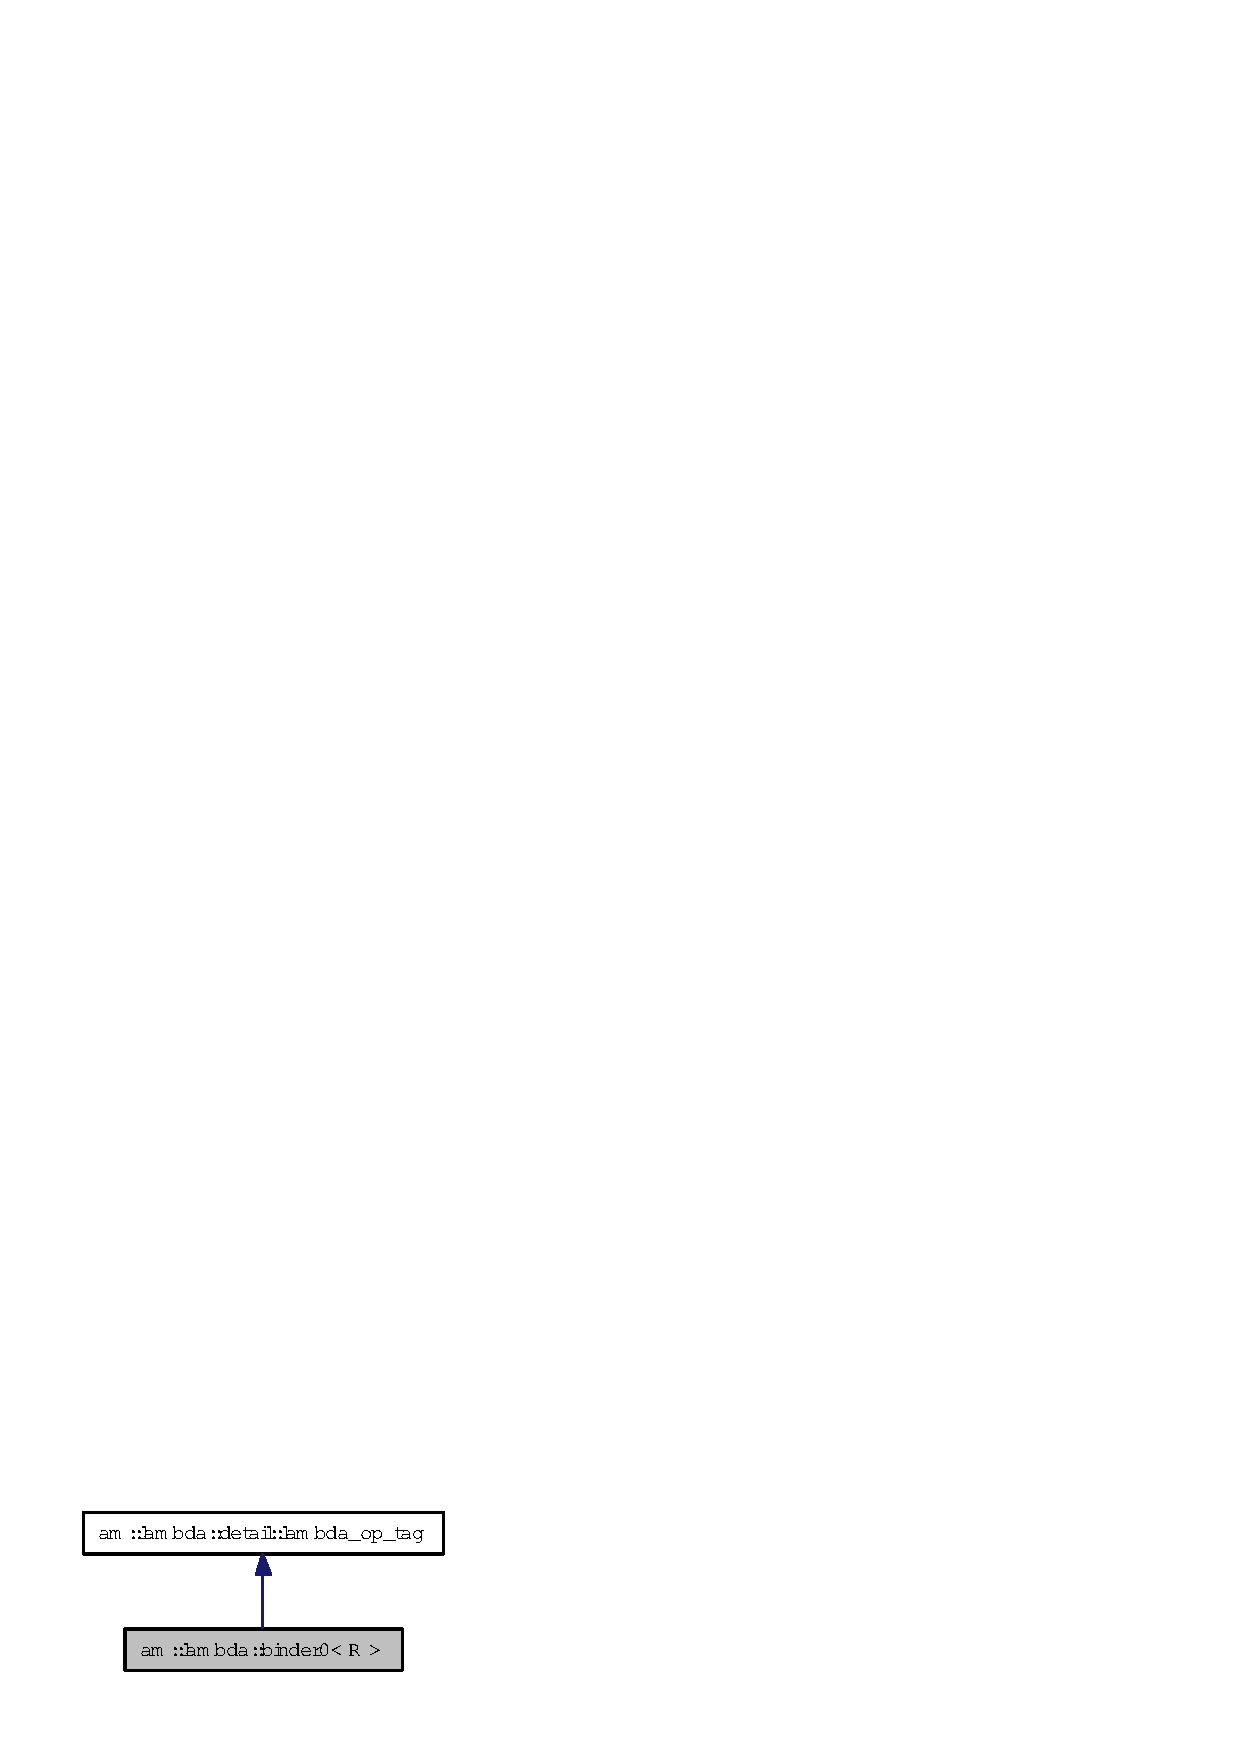
\includegraphics[width=108pt]{structam_1_1lambda_1_1binder0__inherit__graph}
\end{center}
\end{figure}
Collaboration diagram for am::lambda::binder0$<$ R $>$:\begin{figure}[H]
\begin{center}
\leavevmode
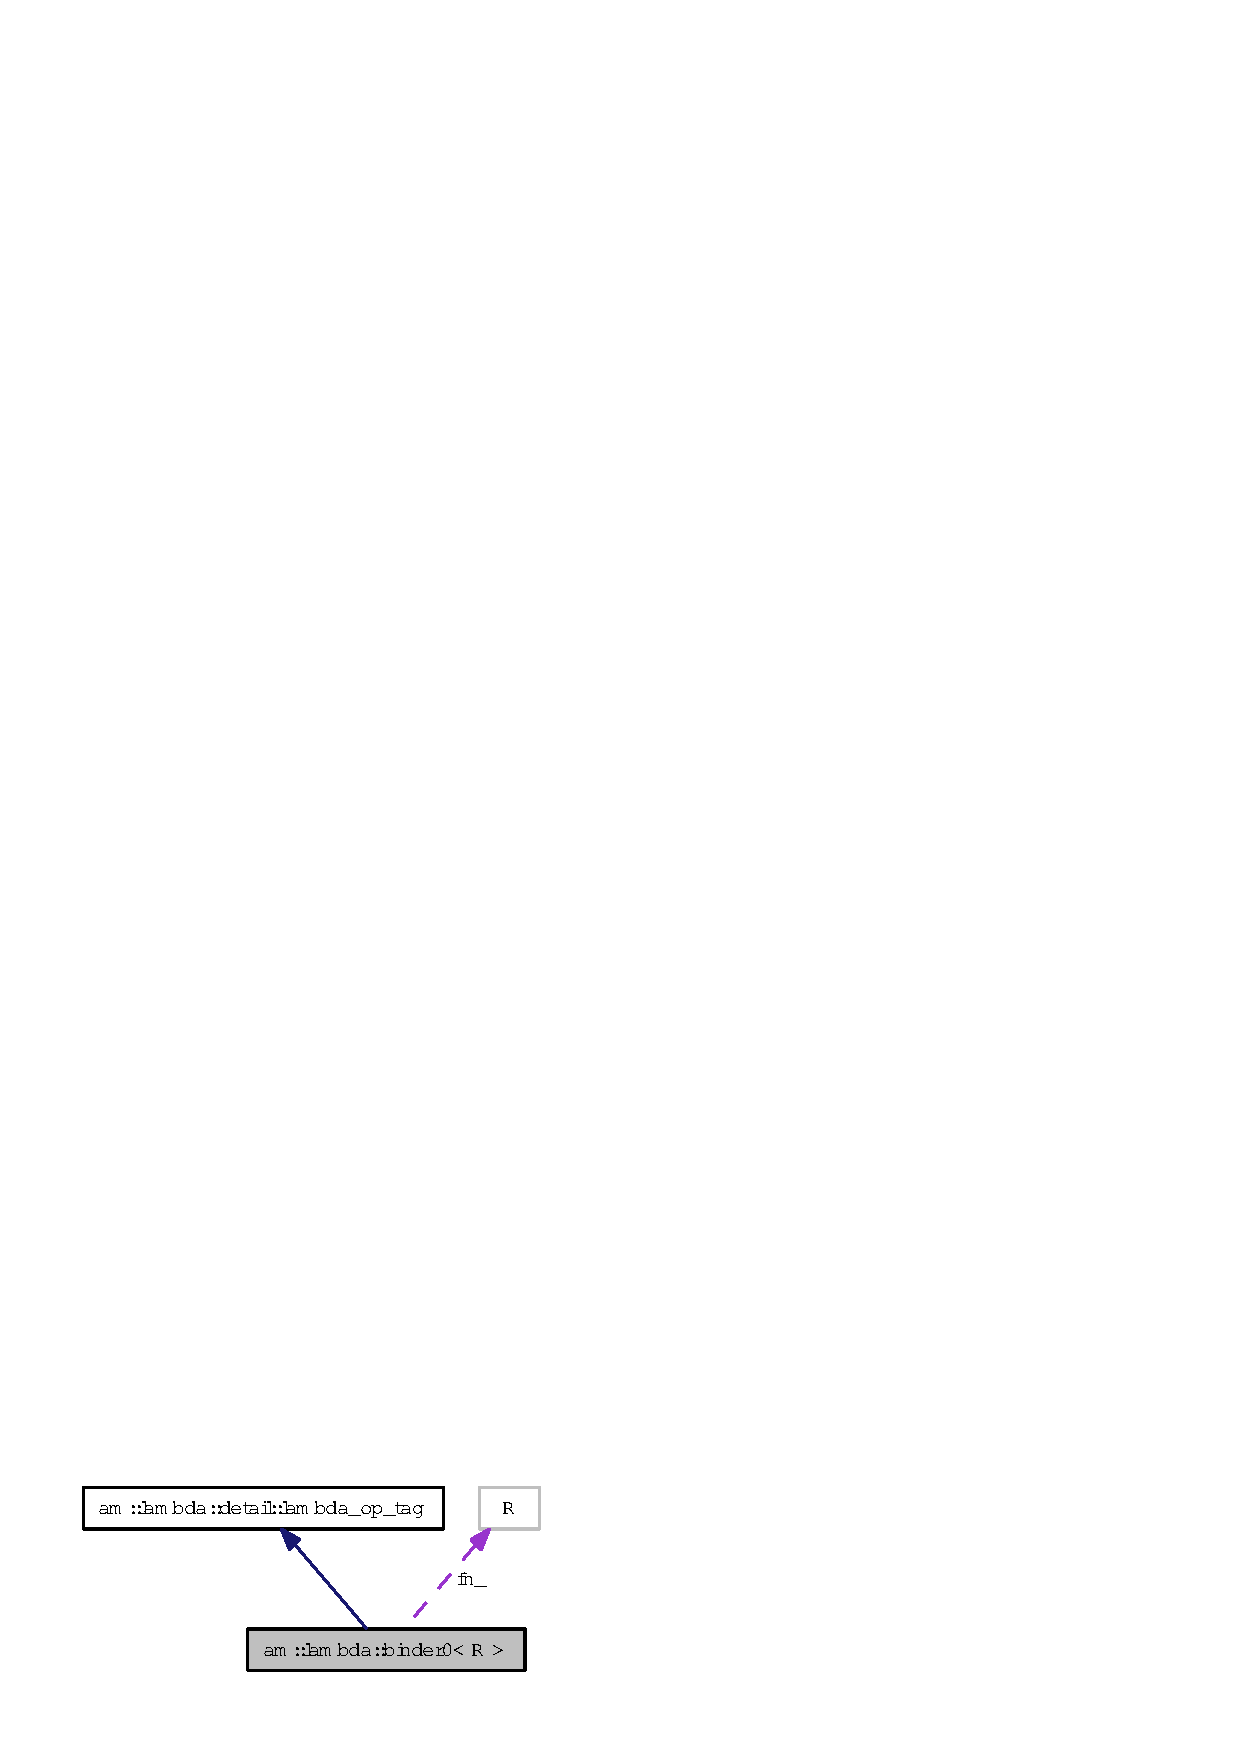
\includegraphics[width=132pt]{structam_1_1lambda_1_1binder0__coll__graph}
\end{center}
\end{figure}
\subsection*{Public Types}
\begin{CompactItemize}
\item 
typedef detail::binder\_\-impl$<$ R $>$::result\_\-type \textbf{result\_\-type}\label{structam_1_1lambda_1_1binder0_dd9b026043ecf5fa477ed0a887e0cae3}

\end{CompactItemize}
\subsection*{Public Member Functions}
\begin{CompactItemize}
\item 
\textbf{binder0} (R($\ast$fn)())\label{structam_1_1lambda_1_1binder0_503871dd93616d4b9fef28c3fcb59794}

\item 
template$<$class T1, class T2, class T3$>$ result\_\-type \textbf{operator()} (T1 t1, T2 t2, T3 t3) const \label{structam_1_1lambda_1_1binder0_140466dec5fe7965454887eea6ccc01b}

\item 
template$<$class T1, class T2$>$ result\_\-type \textbf{operator()} (T1 t1, T2 t2) const\label{structam_1_1lambda_1_1binder0_e6af6516938a98c05aa3f74b296c01d9}

\item 
template$<$class T1$>$ result\_\-type \textbf{operator()} (T1 t1) const \label{structam_1_1lambda_1_1binder0_69732777801aca26cb708730366b78bb}

\item 
result\_\-type \textbf{operator()} () const\label{structam_1_1lambda_1_1binder0_bf97e5aae6c88c14a03775ae1458d037}

\end{CompactItemize}
\subsection*{Public Attributes}
\begin{CompactItemize}
\item 
R($\ast$ \textbf{fn\_\-} )()\label{structam_1_1lambda_1_1binder0_1d5bd3720645f4288bfe02e1658cfcd0}

\end{CompactItemize}


\subsection{Detailed Description}
\subsubsection*{template$<$typename R$>$ struct am::lambda::binder0$<$ R $>$}

Binder for the free function which takes no argument. 



The documentation for this struct was generated from the following file:\begin{CompactItemize}
\item 
{\bf lambda.hpp}\end{CompactItemize}

\section{am::lambda::binder1$<$ R, P1, A1 $>$ Struct Template Reference}
\label{structam_1_1lambda_1_1binder1}\index{am::lambda::binder1@{am::lambda::binder1}}
{\tt \#include $<$lambda.hpp$>$}

Inherits {\bf am::lambda::detail::lambda\_\-op\_\-tag}.

Inheritance diagram for am::lambda::binder1$<$ R, P1, A1 $>$:\begin{figure}[H]
\begin{center}
\leavevmode
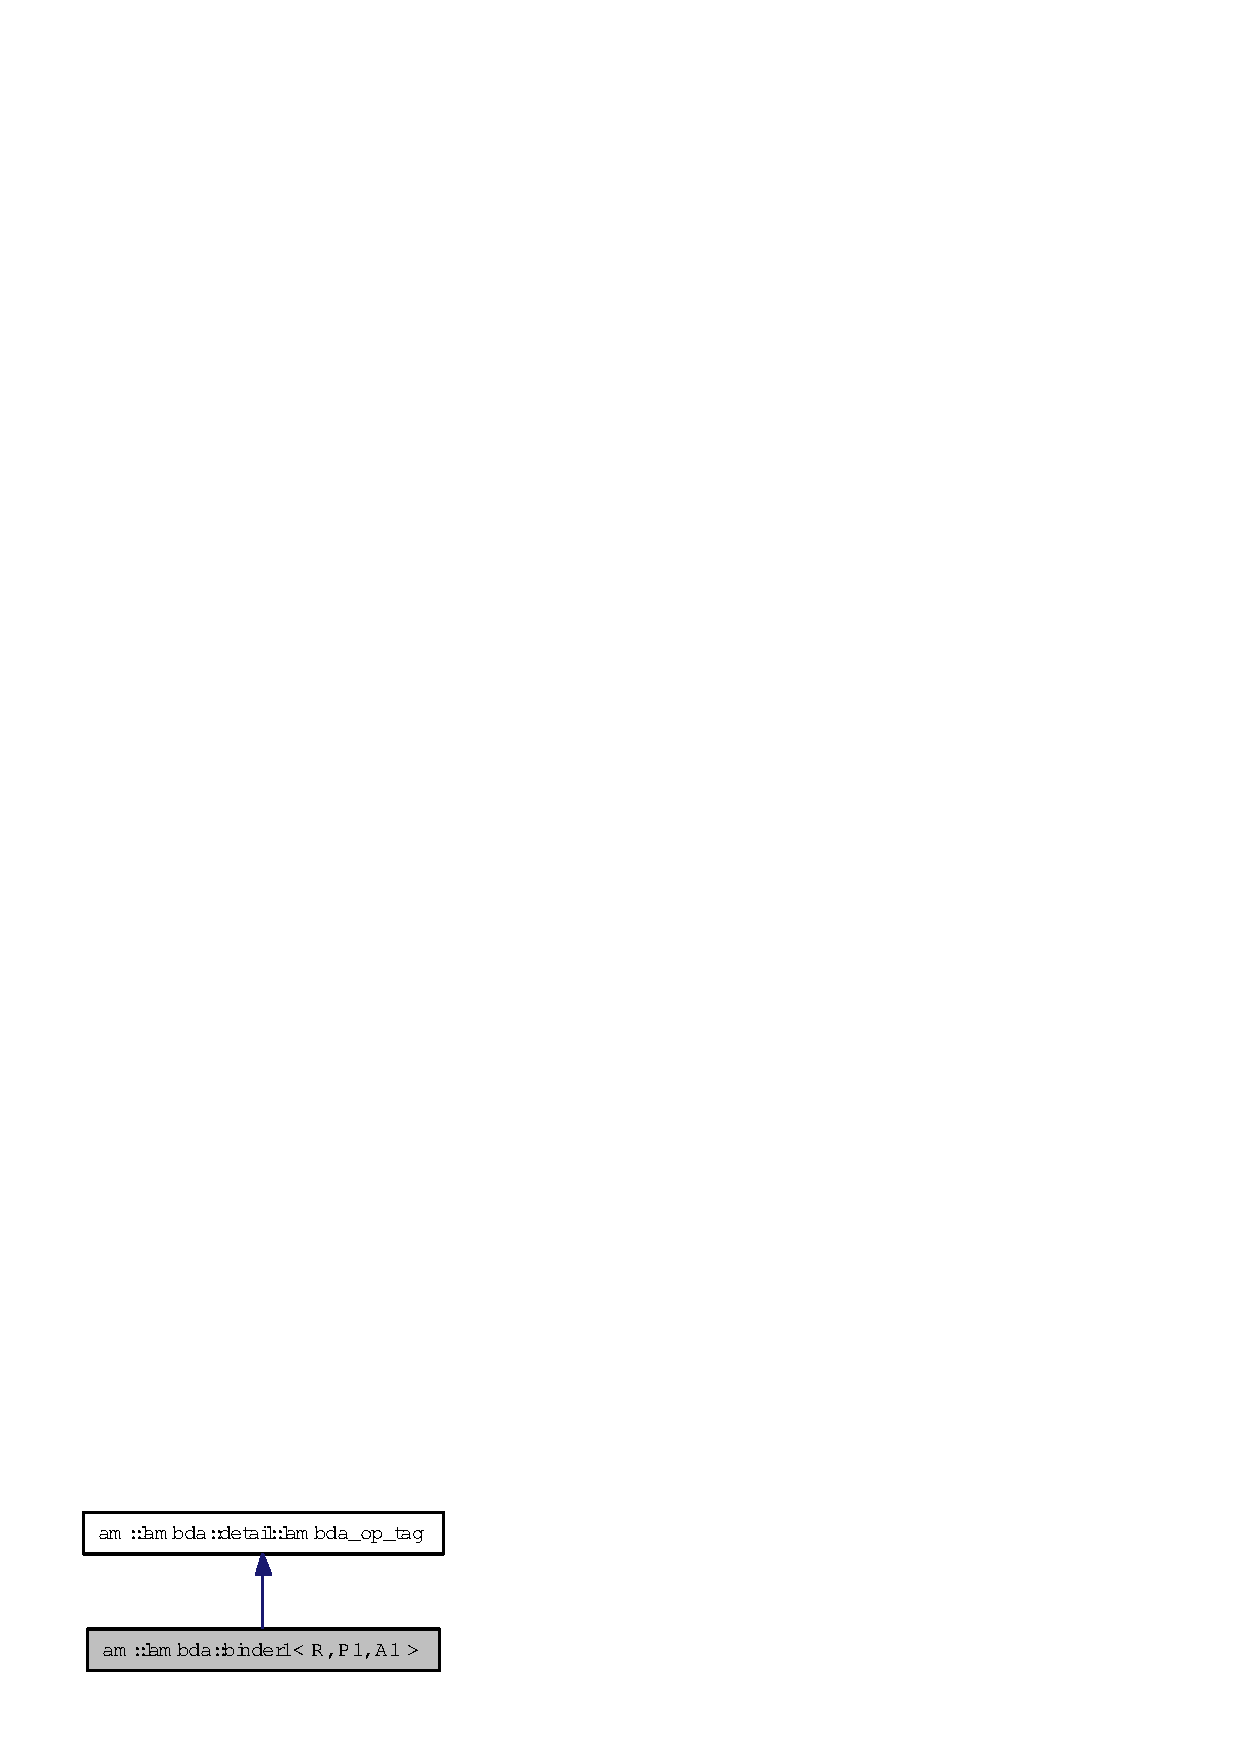
\includegraphics[width=108pt]{structam_1_1lambda_1_1binder1__inherit__graph}
\end{center}
\end{figure}
Collaboration diagram for am::lambda::binder1$<$ R, P1, A1 $>$:\begin{figure}[H]
\begin{center}
\leavevmode
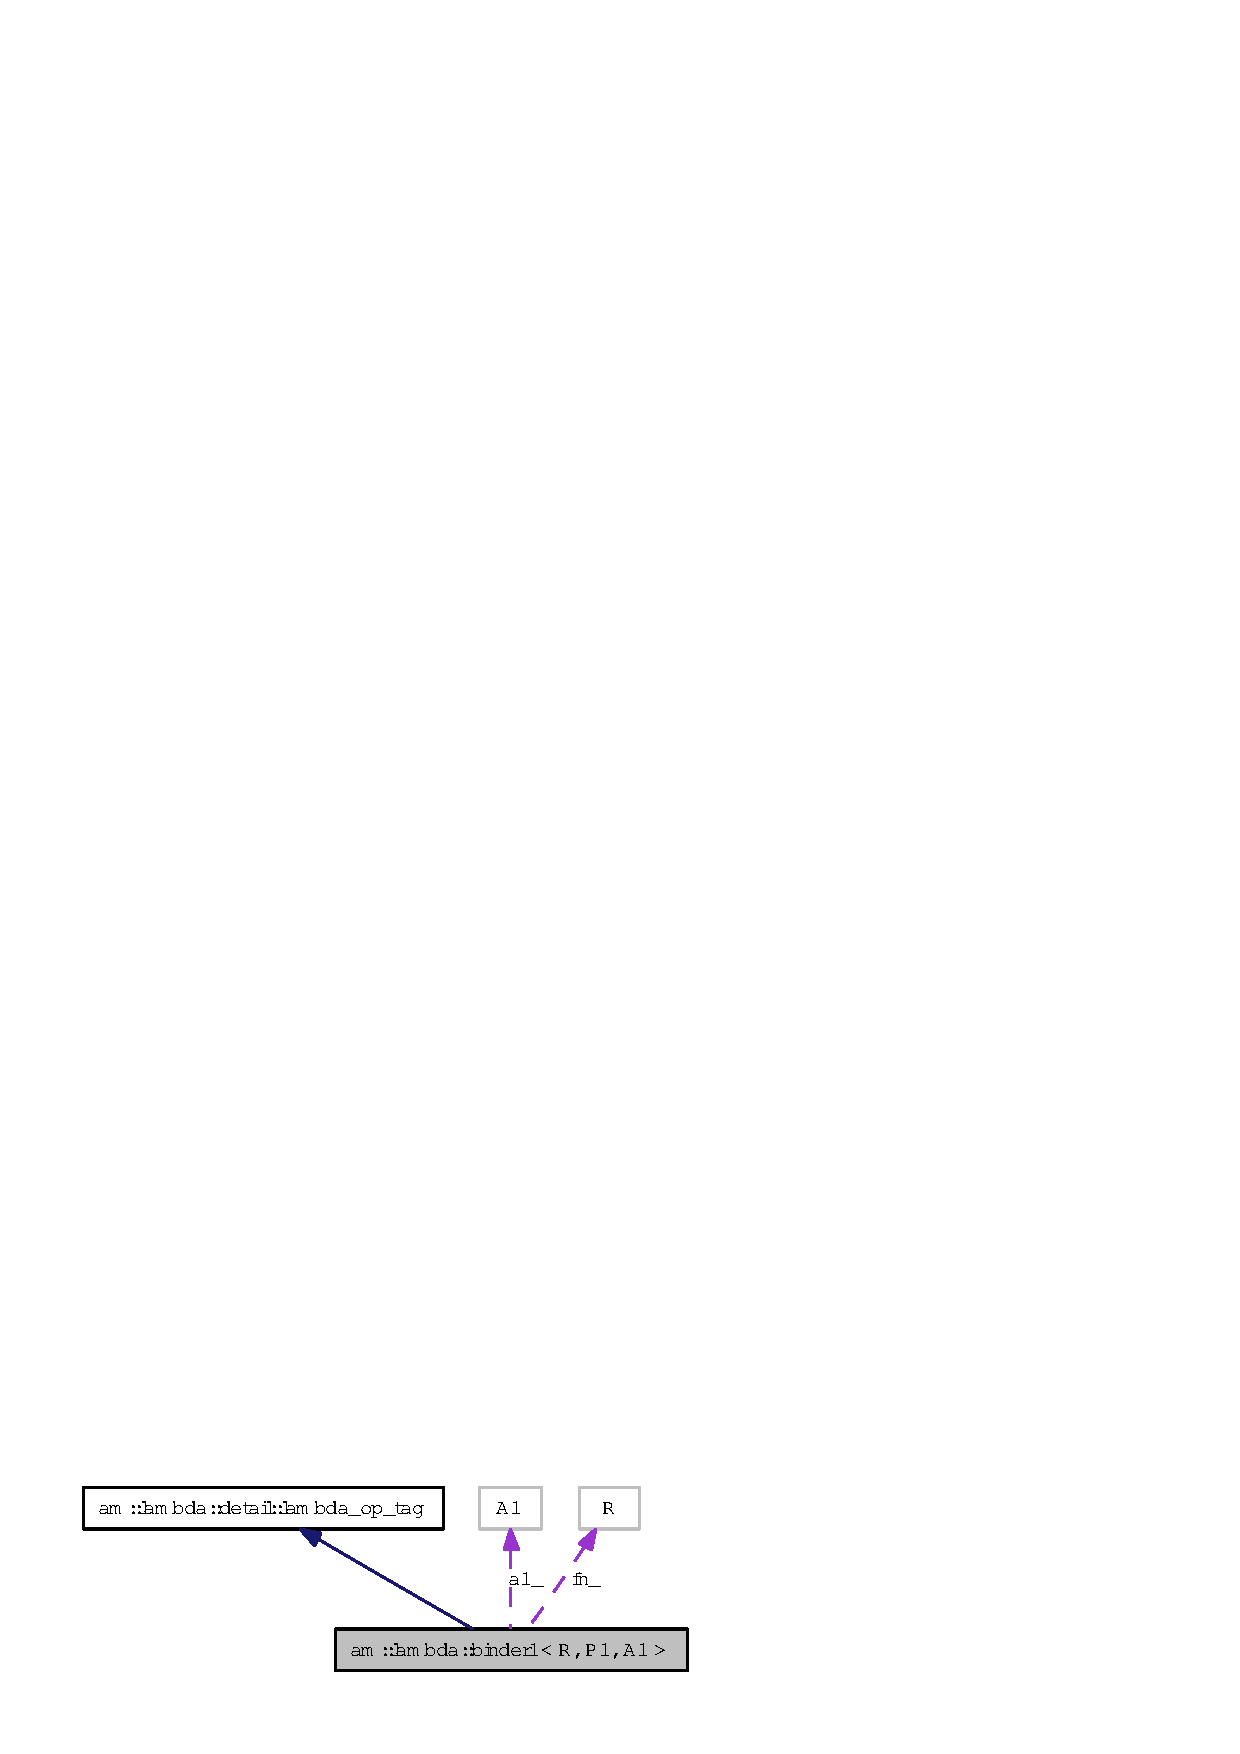
\includegraphics[width=166pt]{structam_1_1lambda_1_1binder1__coll__graph}
\end{center}
\end{figure}
\subsection*{Public Types}
\begin{CompactItemize}
\item 
typedef detail::binder\_\-impl$<$ R $>$::result\_\-type \textbf{result\_\-type}\label{structam_1_1lambda_1_1binder1_9ca2fec190c6c2d883b66b4d3522c95b}

\end{CompactItemize}
\subsection*{Public Member Functions}
\begin{CompactItemize}
\item 
\textbf{binder1} (R($\ast$fn)(P1), A1 a1)\label{structam_1_1lambda_1_1binder1_c2108aaef80abd01a31bce2a0e38c6a3}

\item 
template$<$class T1, class T2, class T3$>$ result\_\-type \textbf{operator()} (T1 t1, T2 t2, T3 t3) const \label{structam_1_1lambda_1_1binder1_480bdebf86834c60e81bd98e82ae1eb9}

\item 
template$<$class T1, class T2$>$ result\_\-type \textbf{operator()} (T1 t1, T2 t2) const\label{structam_1_1lambda_1_1binder1_e3b600bffd6e5564189362b838a5e341}

\item 
template$<$class T1$>$ result\_\-type \textbf{operator()} (T1 t1) const \label{structam_1_1lambda_1_1binder1_2f055604a17c90630328a6fe236387d4}

\item 
result\_\-type \textbf{operator()} () const\label{structam_1_1lambda_1_1binder1_1238e7e2aec16f220493f12e385c5808}

\end{CompactItemize}
\subsection*{Public Attributes}
\begin{CompactItemize}
\item 
R($\ast$ \textbf{fn\_\-} )(P1)\label{structam_1_1lambda_1_1binder1_54e5220f72cf932262c966ed61ba42fb}

\item 
A1 \textbf{a1\_\-}\label{structam_1_1lambda_1_1binder1_e83629cd1c47a8a452918e8b6bc12845}

\end{CompactItemize}


\subsection{Detailed Description}
\subsubsection*{template$<$typename R, typename P1, typename A1$>$ struct am::lambda::binder1$<$ R, P1, A1 $>$}

Binder for the free function which takes one argument. 



The documentation for this struct was generated from the following file:\begin{CompactItemize}
\item 
{\bf lambda.hpp}\end{CompactItemize}

\section{am::binder1st$<$ Op, P1 $>$ Struct Template Reference}
\label{structam_1_1binder1st}\index{am::binder1st@{am::binder1st}}
Bind the 1st argument of a binary function.  


{\tt \#include $<$mate.hpp$>$}

Collaboration diagram for am::binder1st$<$ Op, P1 $>$:\begin{figure}[H]
\begin{center}
\leavevmode
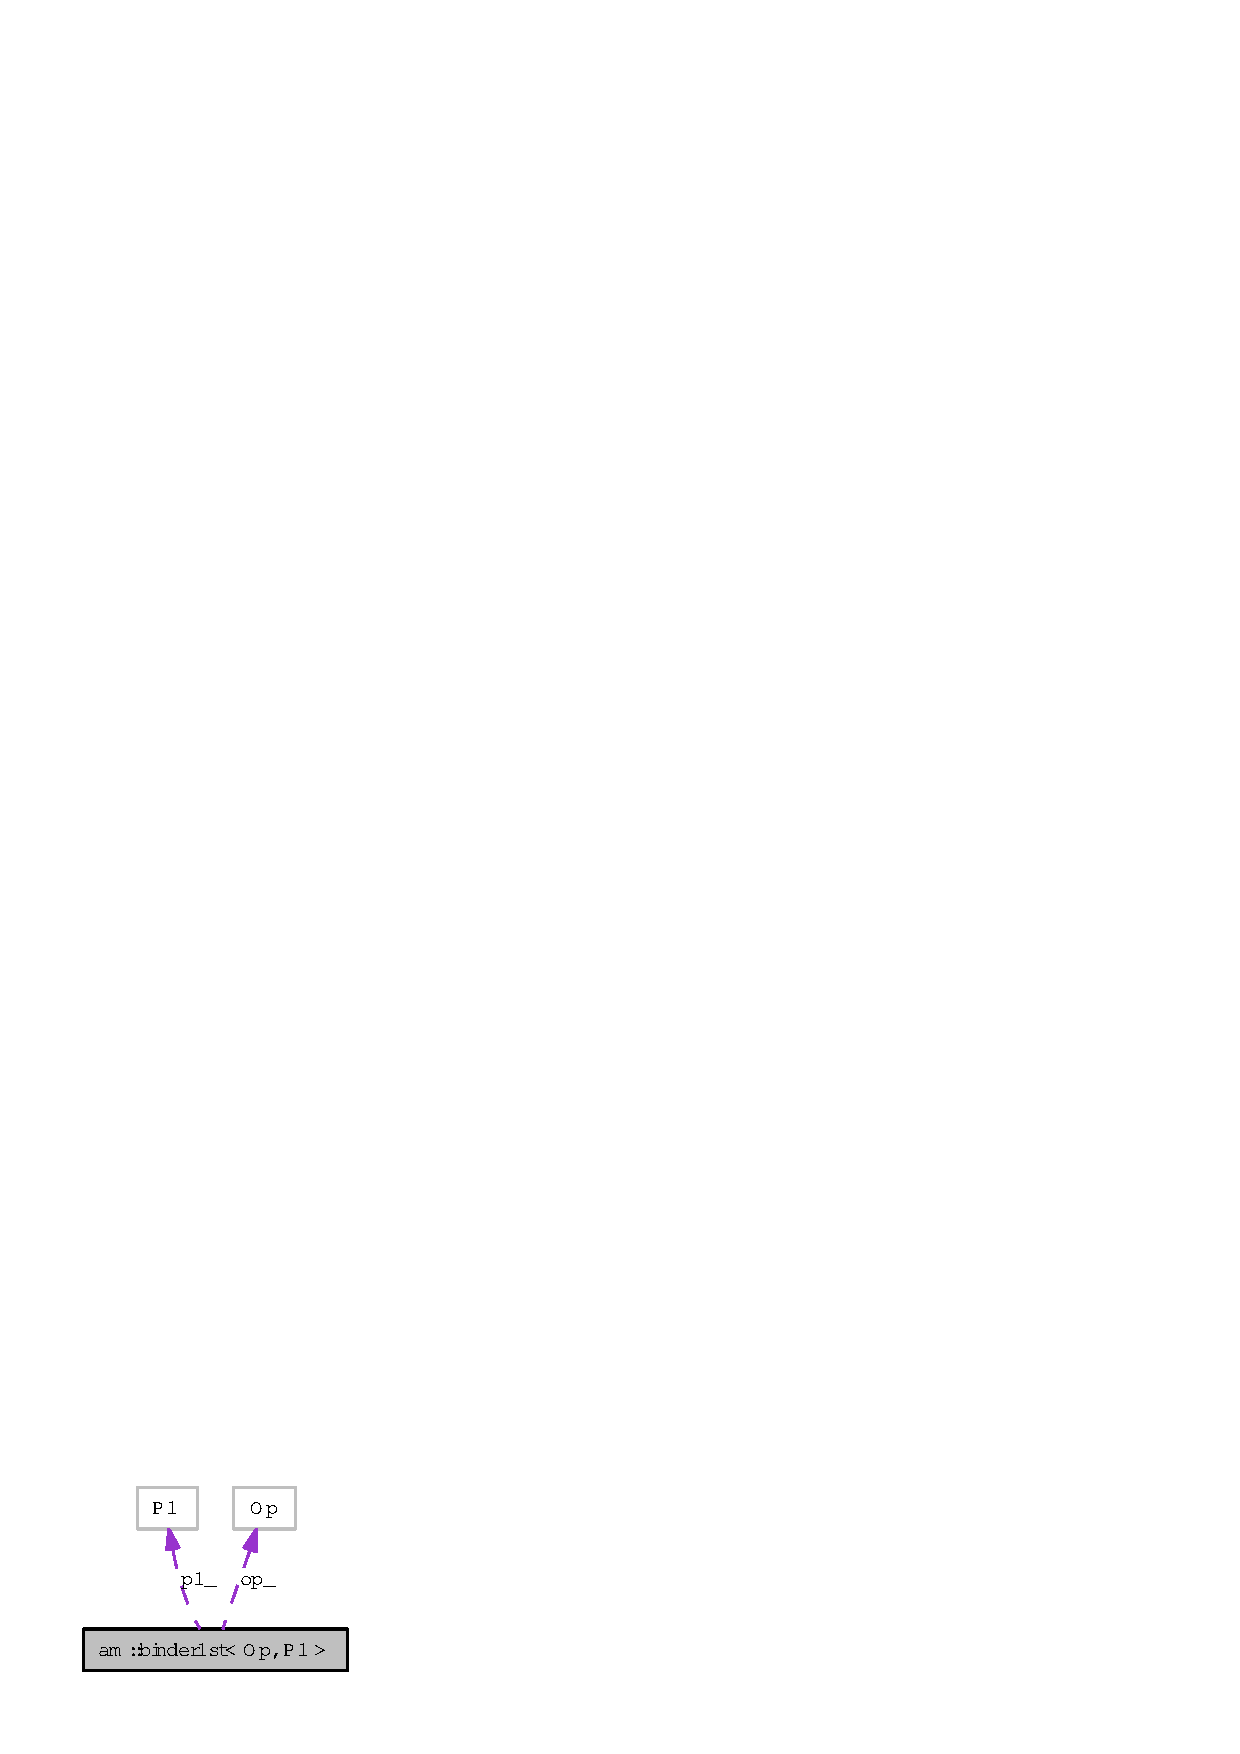
\includegraphics[width=85pt]{structam_1_1binder1st__coll__graph}
\end{center}
\end{figure}
\subsection*{Public Types}
\begin{CompactItemize}
\item 
typedef void \textbf{result\_\-type}\label{structam_1_1binder1st_919162b1f1ed1a60fb8326d1d6b6a2e9}

\end{CompactItemize}
\subsection*{Public Member Functions}
\begin{CompactItemize}
\item 
\textbf{binder1st} (Op const \&op, P1 p1)\label{structam_1_1binder1st_64cd9ea585cadbd8bed866e506b741f7}

\item 
template$<$typename P2$>$ void \textbf{operator()} (P2 p2) const \label{structam_1_1binder1st_8a293442627728c93e96fba4ffa5697f}

\end{CompactItemize}
\subsection*{Public Attributes}
\begin{CompactItemize}
\item 
Op const \& \textbf{op\_\-}\label{structam_1_1binder1st_6a17e636556d6ef2097700eff9a33ff7}

\item 
P1 \textbf{p1\_\-}\label{structam_1_1binder1st_efd3c635a67fe43ced707bfad9f655a2}

\end{CompactItemize}


\subsection{Detailed Description}
\subsubsection*{template$<$typename Op, typename P1$>$ struct am::binder1st$<$ Op, P1 $>$}

Bind the 1st argument of a binary function. 

It is not a std::unary\_\-function, but works for any calling convention.

\begin{Desc}
\item[See also:]\doxyref{bind1st()}{p.}{namespaceam_5d35d0139360afc672d2cf1ff279fd83} \end{Desc}




The documentation for this struct was generated from the following file:\begin{CompactItemize}
\item 
{\bf mate.hpp}\end{CompactItemize}

\section{am::lambda::binder2$<$ R, P1, P2, A1, A2 $>$ Struct Template Reference}
\label{structam_1_1lambda_1_1binder2}\index{am::lambda::binder2@{am::lambda::binder2}}
{\tt \#include $<$lambda.hpp$>$}

Inherits {\bf am::lambda::detail::lambda\_\-op\_\-tag}.

Inheritance diagram for am::lambda::binder2$<$ R, P1, P2, A1, A2 $>$:\begin{figure}[H]
\begin{center}
\leavevmode
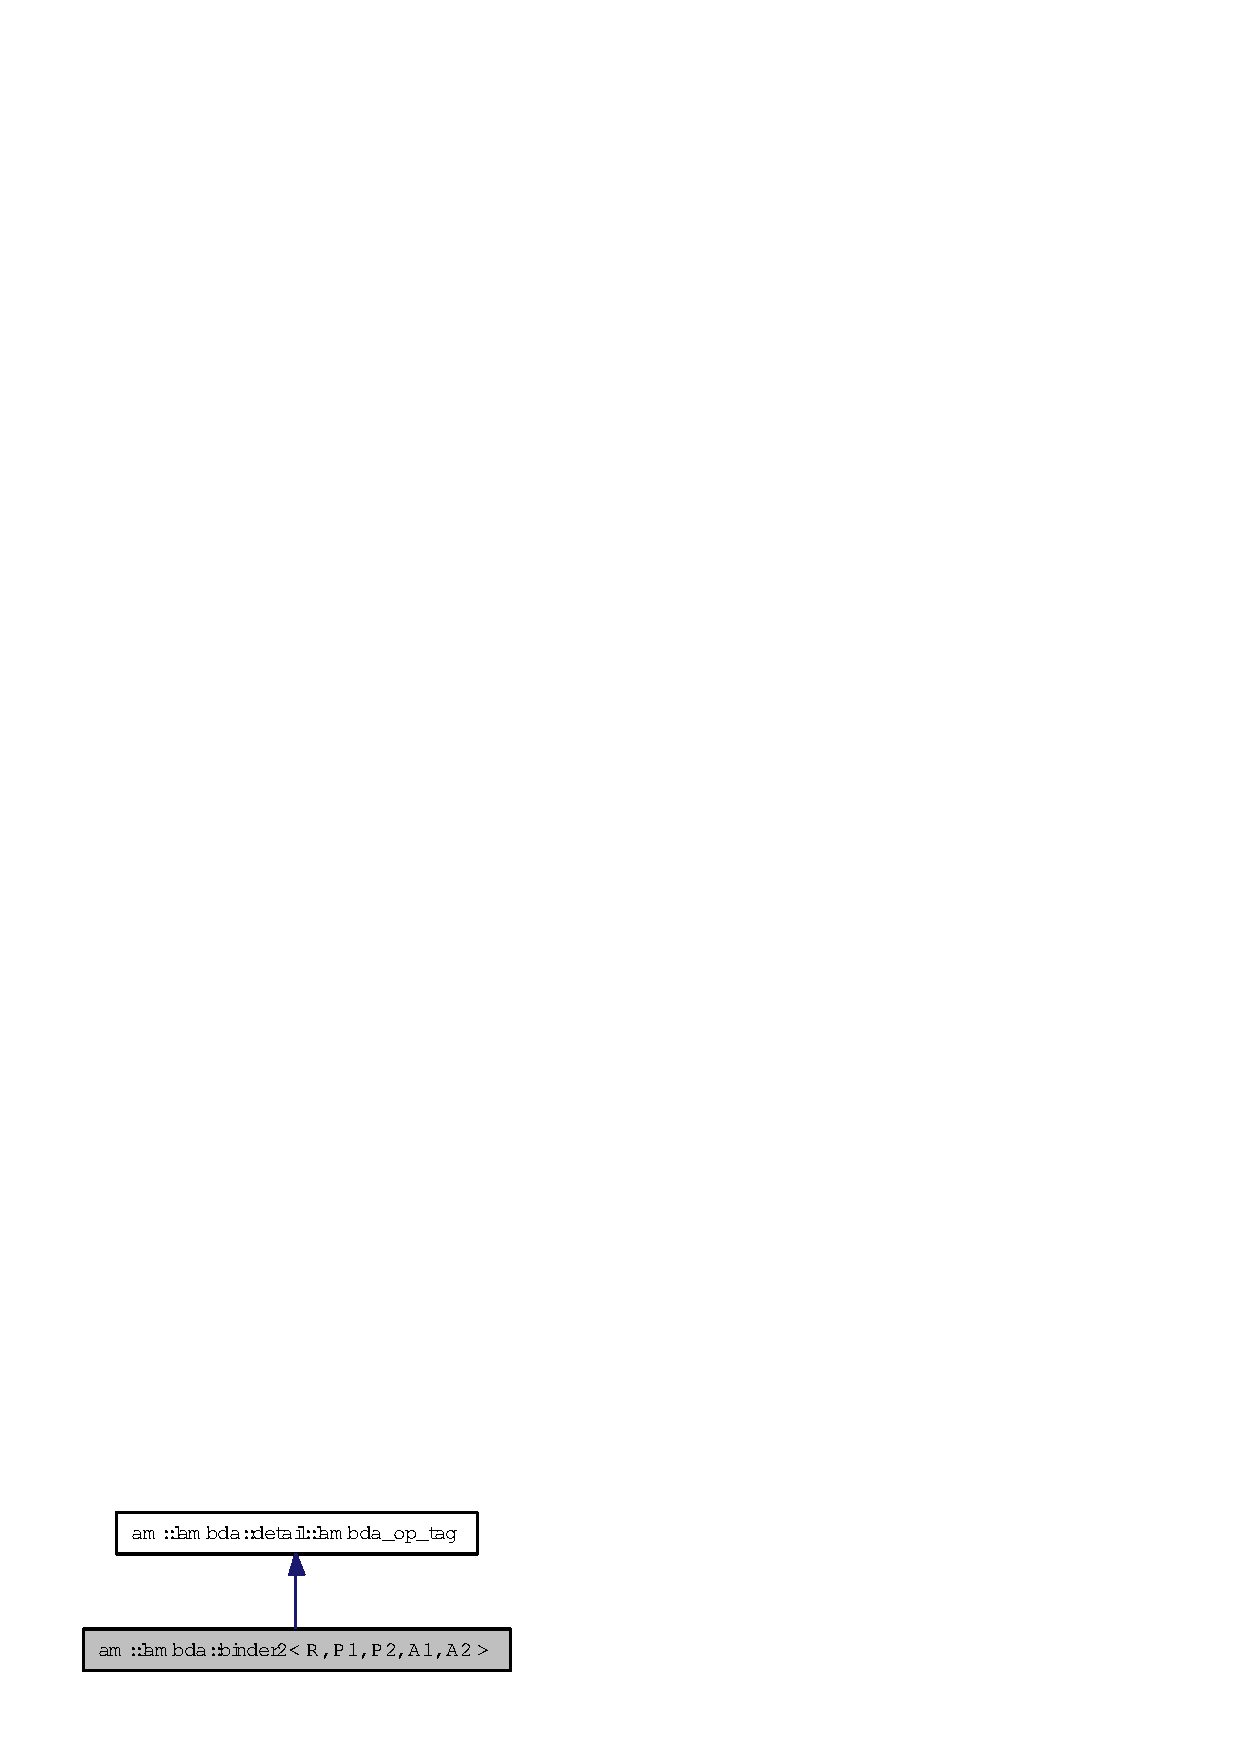
\includegraphics[width=124pt]{structam_1_1lambda_1_1binder2__inherit__graph}
\end{center}
\end{figure}
Collaboration diagram for am::lambda::binder2$<$ R, P1, P2, A1, A2 $>$:\begin{figure}[H]
\begin{center}
\leavevmode
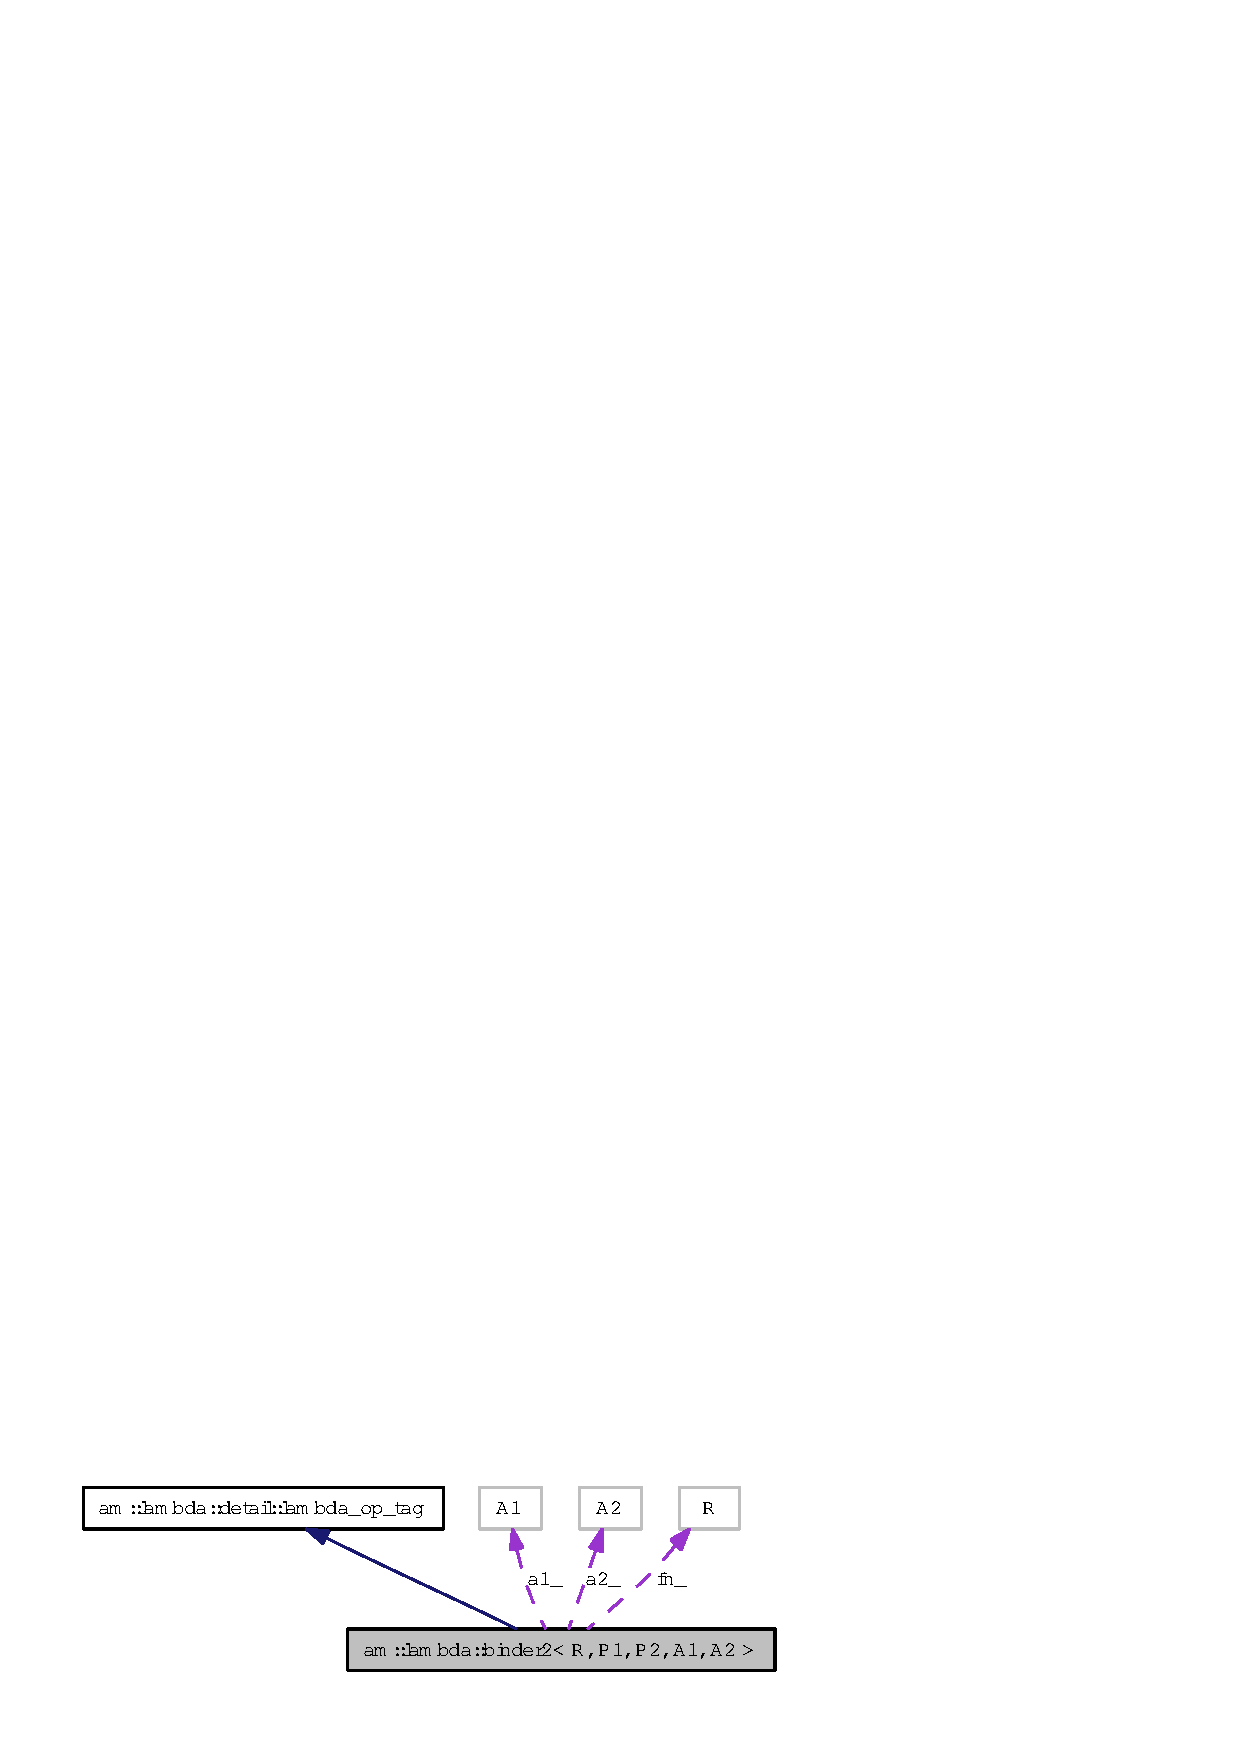
\includegraphics[width=187pt]{structam_1_1lambda_1_1binder2__coll__graph}
\end{center}
\end{figure}
\subsection*{Public Types}
\begin{CompactItemize}
\item 
typedef detail::binder\_\-impl$<$ R $>$::result\_\-type \textbf{result\_\-type}\label{structam_1_1lambda_1_1binder2_d73405ab552afa44c840d27cd4709304}

\end{CompactItemize}
\subsection*{Public Member Functions}
\begin{CompactItemize}
\item 
\textbf{binder2} (R($\ast$fn)(P1, P2), A1 a1, A2 a2)\label{structam_1_1lambda_1_1binder2_4d517a5e99db7eb10225d490c802fa74}

\item 
template$<$class T1, class T2, class T3$>$ result\_\-type \textbf{operator()} (T1 t1, T2 t2, T3 t3) const \label{structam_1_1lambda_1_1binder2_8c204abc6133be2e95cd176639f52448}

\item 
template$<$class T1, class T2$>$ result\_\-type \textbf{operator()} (T1 t1, T2 t2) const\label{structam_1_1lambda_1_1binder2_2019db2e2568b959a5e5f5ad3b77f900}

\item 
template$<$class T1$>$ result\_\-type \textbf{operator()} (T1 t1) const \label{structam_1_1lambda_1_1binder2_3576ec06cf7e48b3b7346eeeecbb20dc}

\item 
result\_\-type \textbf{operator()} () const\label{structam_1_1lambda_1_1binder2_08f8cf7c190fc6e5e46e13010a9a86f9}

\end{CompactItemize}
\subsection*{Public Attributes}
\begin{CompactItemize}
\item 
R($\ast$ \textbf{fn\_\-} )(P1, P2)\label{structam_1_1lambda_1_1binder2_b214a0c003ee4e9c8ac97fda0bca30a9}

\item 
A1 \textbf{a1\_\-}\label{structam_1_1lambda_1_1binder2_ce8184c78e50af5a002839aba6b1351a}

\item 
A2 \textbf{a2\_\-}\label{structam_1_1lambda_1_1binder2_0de68b465afbb45b7304a96a1f6d671a}

\end{CompactItemize}


\subsection{Detailed Description}
\subsubsection*{template$<$typename R, typename P1, typename P2, typename A1, typename A2$>$ struct am::lambda::binder2$<$ R, P1, P2, A1, A2 $>$}

Binder for the free function which takes two arguments. 



The documentation for this struct was generated from the following file:\begin{CompactItemize}
\item 
{\bf lambda.hpp}\end{CompactItemize}

\section{am::binder2nd$<$ Op, P2 $>$ Struct Template Reference}
\label{structam_1_1binder2nd}\index{am::binder2nd@{am::binder2nd}}
Bind the 2nd argument of a binary function.  


{\tt \#include $<$mate.hpp$>$}

Collaboration diagram for am::binder2nd$<$ Op, P2 $>$:\begin{figure}[H]
\begin{center}
\leavevmode
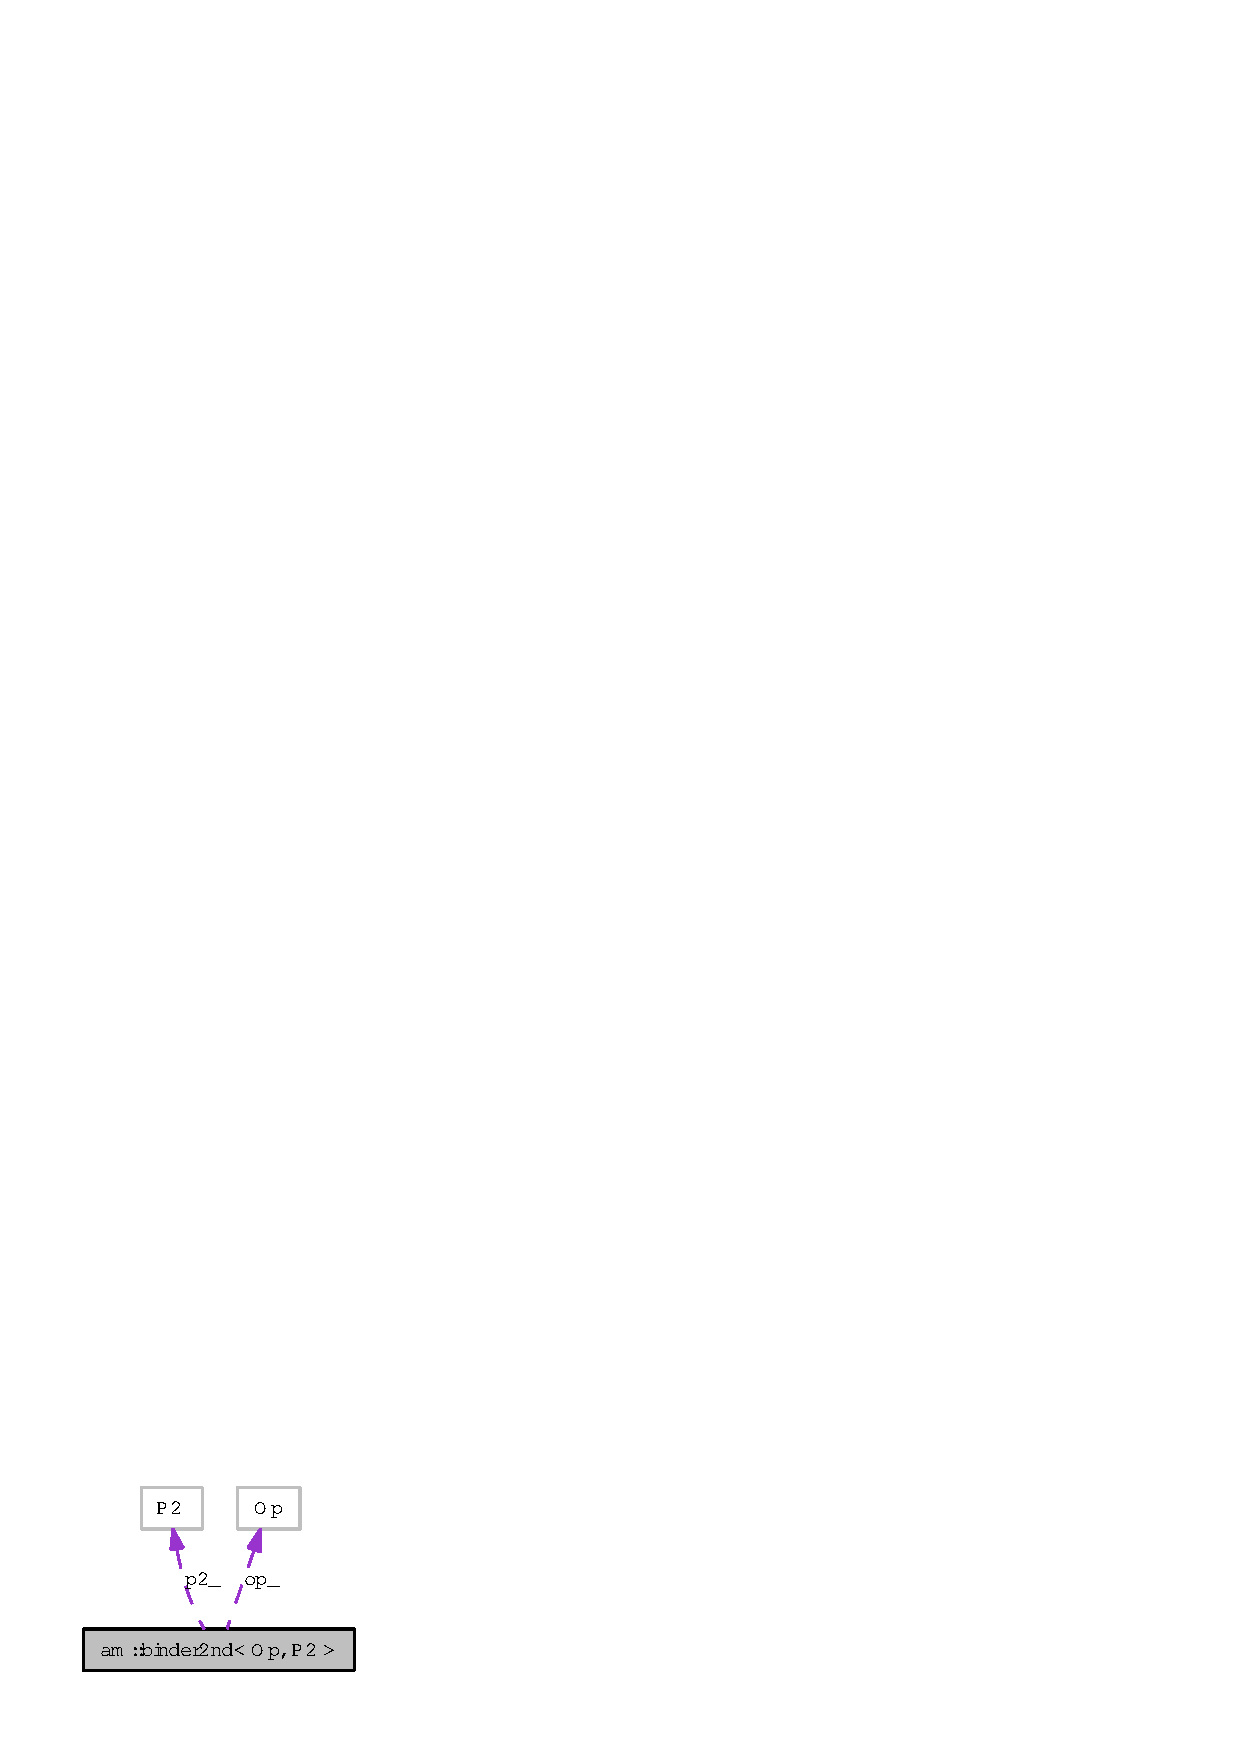
\includegraphics[width=87pt]{structam_1_1binder2nd__coll__graph}
\end{center}
\end{figure}
\subsection*{Public Types}
\begin{CompactItemize}
\item 
typedef void \textbf{result\_\-type}\label{structam_1_1binder2nd_c110dbaaaf87a6572bc4963c48965fbe}

\end{CompactItemize}
\subsection*{Public Member Functions}
\begin{CompactItemize}
\item 
\textbf{binder2nd} (Op const \&op, P2 p2)\label{structam_1_1binder2nd_a912b086eb789f7f18a455309289ed6f}

\item 
template$<$typename P1$>$ void \textbf{operator()} (P1 p1) const \label{structam_1_1binder2nd_fad651369499f2e03e9815c8a0f2bd50}

\end{CompactItemize}
\subsection*{Public Attributes}
\begin{CompactItemize}
\item 
Op const \& \textbf{op\_\-}\label{structam_1_1binder2nd_80e40f09fb0a1d196bb1a6c795c4d18c}

\item 
P2 \textbf{p2\_\-}\label{structam_1_1binder2nd_3e5b387abf4e245757b45ac4a14d9777}

\end{CompactItemize}


\subsection{Detailed Description}
\subsubsection*{template$<$typename Op, typename P2$>$ struct am::binder2nd$<$ Op, P2 $>$}

Bind the 2nd argument of a binary function. 

It is not a std::unary\_\-function, but works for any calling convention.

\begin{Desc}
\item[See also:]\doxyref{bind2nd()}{p.}{namespaceam_7416ae43749c6a8c08f3a1f8760ae24f} \end{Desc}




The documentation for this struct was generated from the following file:\begin{CompactItemize}
\item 
{\bf mate.hpp}\end{CompactItemize}

\section{am::lambda::binder3$<$ R, P1, P2, P3, A1, A2, A3 $>$ Struct Template Reference}
\label{structam_1_1lambda_1_1binder3}\index{am::lambda::binder3@{am::lambda::binder3}}
{\tt \#include $<$lambda.hpp$>$}

Inherits {\bf am::lambda::detail::lambda\_\-op\_\-tag}.

Inheritance diagram for am::lambda::binder3$<$ R, P1, P2, P3, A1, A2, A3 $>$:\begin{figure}[H]
\begin{center}
\leavevmode
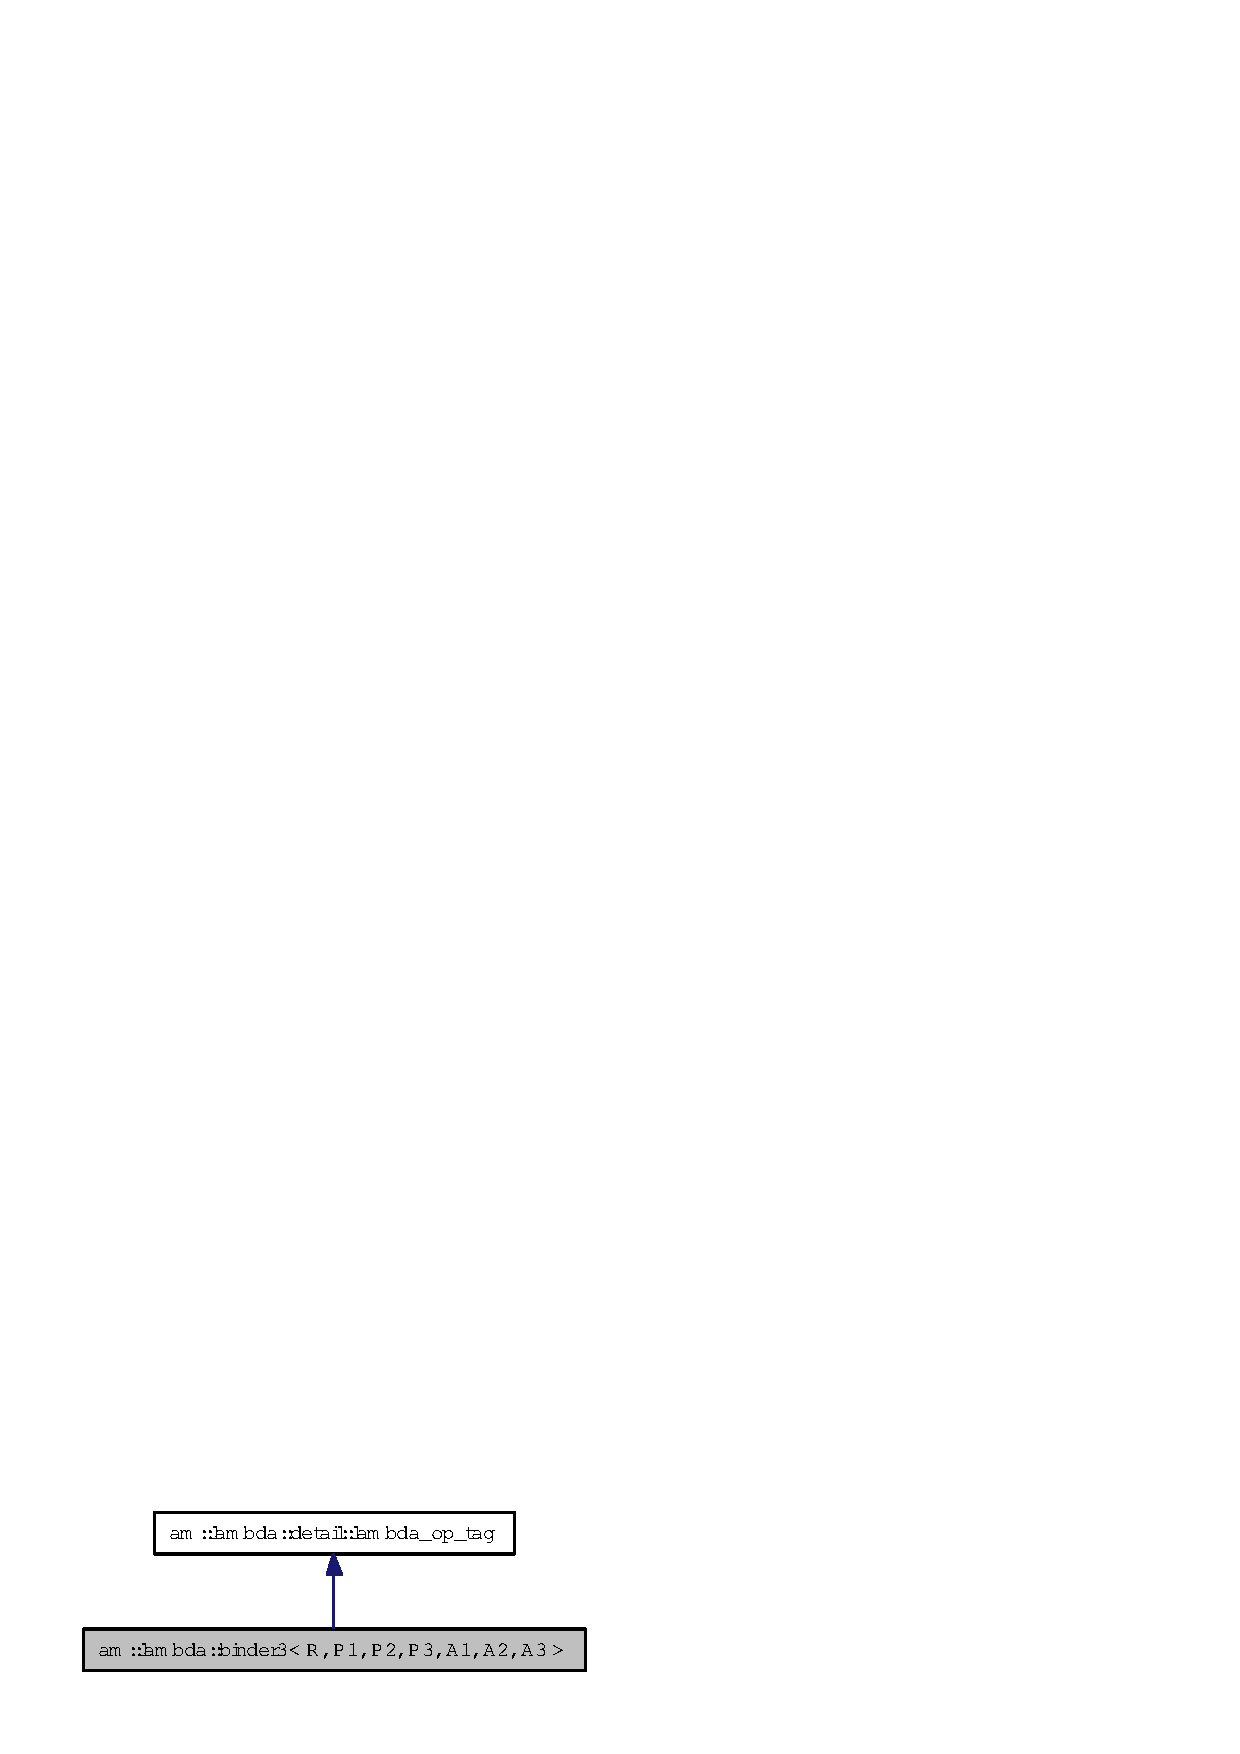
\includegraphics[width=142pt]{structam_1_1lambda_1_1binder3__inherit__graph}
\end{center}
\end{figure}
Collaboration diagram for am::lambda::binder3$<$ R, P1, P2, P3, A1, A2, A3 $>$:\begin{figure}[H]
\begin{center}
\leavevmode
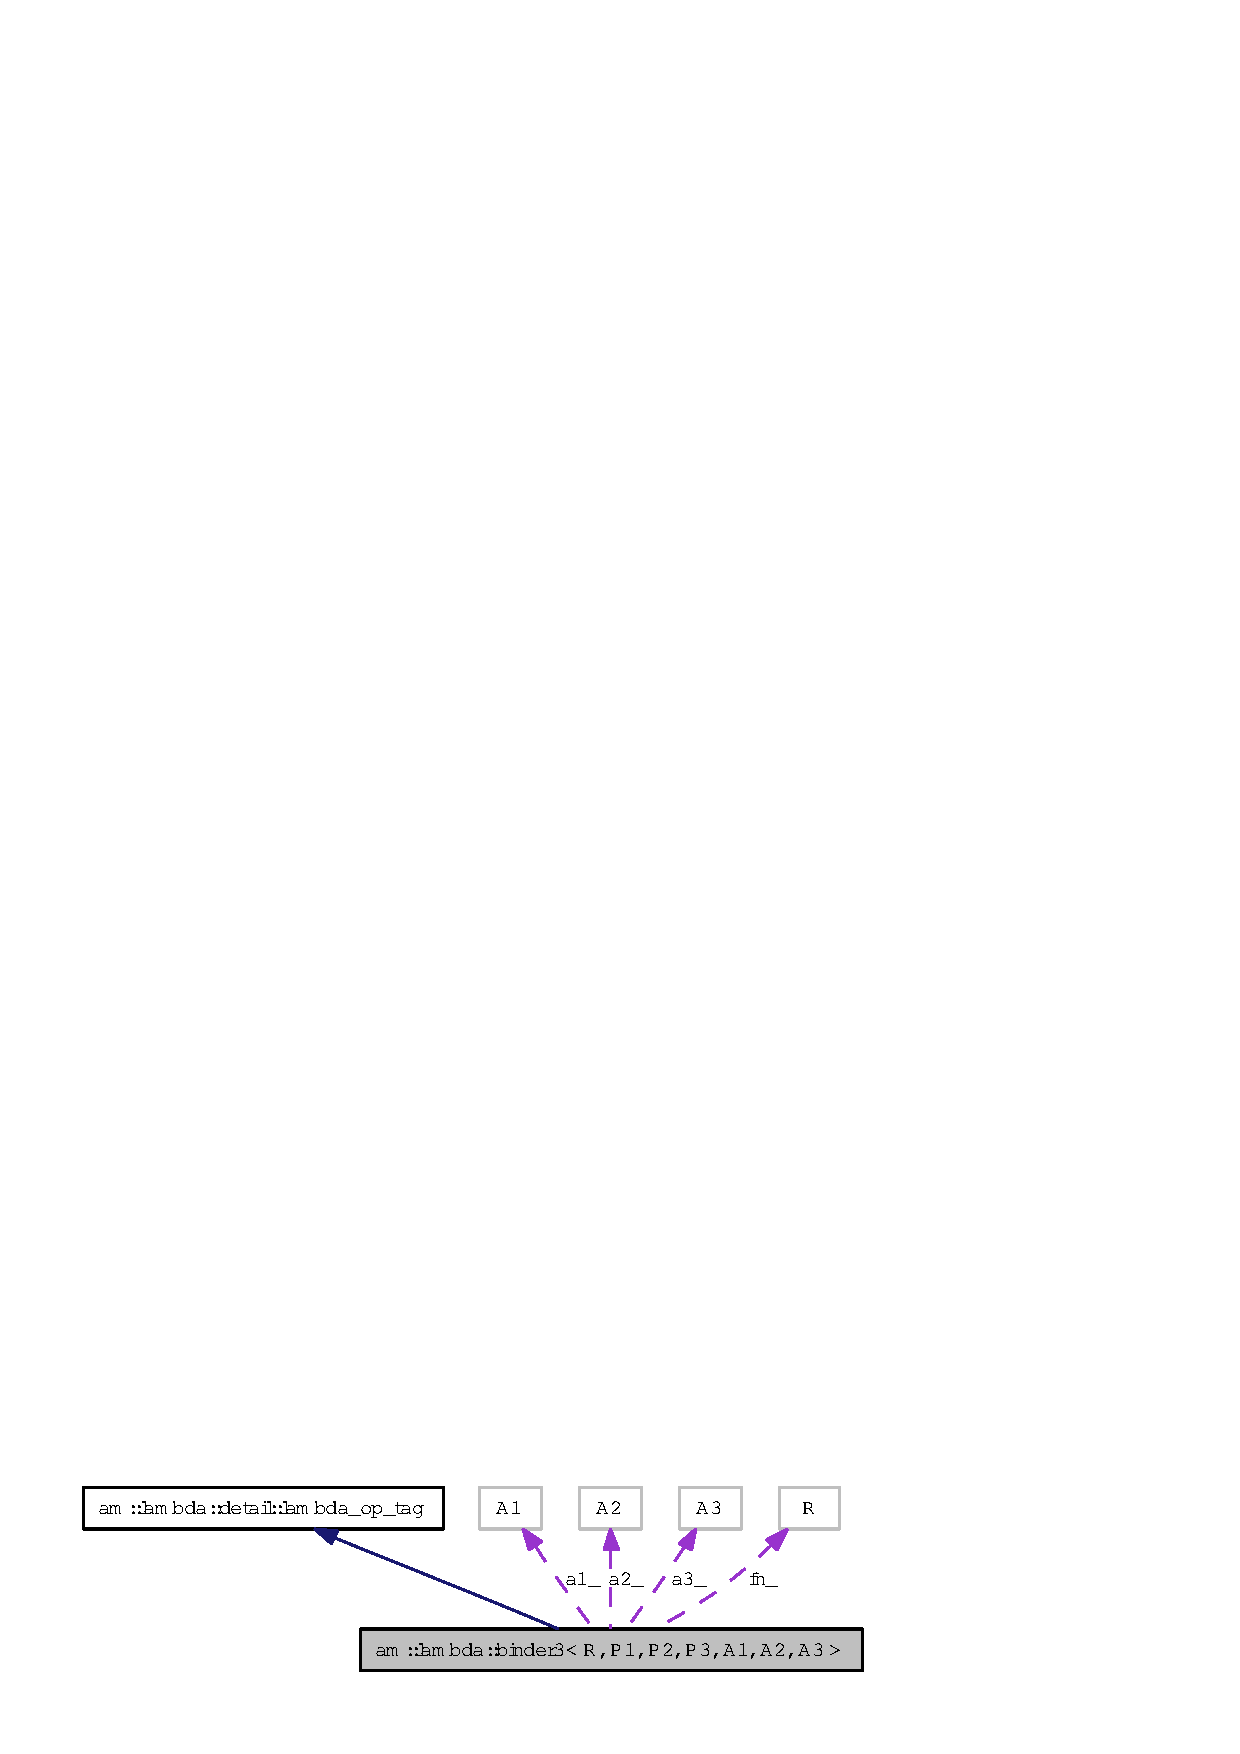
\includegraphics[width=208pt]{structam_1_1lambda_1_1binder3__coll__graph}
\end{center}
\end{figure}
\subsection*{Public Types}
\begin{CompactItemize}
\item 
typedef detail::binder\_\-impl$<$ R $>$::result\_\-type \textbf{result\_\-type}\label{structam_1_1lambda_1_1binder3_4cbe90e647efd7989dedefd02c6d4942}

\end{CompactItemize}
\subsection*{Public Member Functions}
\begin{CompactItemize}
\item 
\textbf{binder3} (R($\ast$fn)(P1, P2, P3), A1 a1, A2 a2, A3 a3)\label{structam_1_1lambda_1_1binder3_0fc64e182ce14a2e0226c4aed7669595}

\item 
template$<$class T1, class T2, class T3$>$ result\_\-type \textbf{operator()} (T1 t1, T2 t2, T3 t3) const \label{structam_1_1lambda_1_1binder3_6e385adbc8d03bb743d036cc66ab5274}

\item 
template$<$class T1, class T2$>$ result\_\-type \textbf{operator()} (T1 t1, T2 t2) const\label{structam_1_1lambda_1_1binder3_2820f406391aee3c5dcaa3698745d2d9}

\item 
template$<$class T1$>$ result\_\-type \textbf{operator()} (T1 t1) const \label{structam_1_1lambda_1_1binder3_88038d1817a18b61ead1ec513ee6e291}

\item 
result\_\-type \textbf{operator()} () const\label{structam_1_1lambda_1_1binder3_6281d09b9414009f2428e22f6b282cb7}

\end{CompactItemize}
\subsection*{Public Attributes}
\begin{CompactItemize}
\item 
R($\ast$ \textbf{fn\_\-} )(P1, P2, P3)\label{structam_1_1lambda_1_1binder3_11ea57f8e411cf238142c8893d59d9c6}

\item 
A1 \textbf{a1\_\-}\label{structam_1_1lambda_1_1binder3_2e578b8d898e9221094c6ef64362aa98}

\item 
A2 \textbf{a2\_\-}\label{structam_1_1lambda_1_1binder3_fcf561d9b972eb387ad91b0c6c605e71}

\item 
A3 \textbf{a3\_\-}\label{structam_1_1lambda_1_1binder3_94d9591a62e2343b0889c57ada1511e0}

\end{CompactItemize}


\subsection{Detailed Description}
\subsubsection*{template$<$typename R, typename P1, typename P2, typename P3, typename A1, typename A2, typename A3$>$ struct am::lambda::binder3$<$ R, P1, P2, P3, A1, A2, A3 $>$}

Binder for the free function which takes three arguments. 



The documentation for this struct was generated from the following file:\begin{CompactItemize}
\item 
{\bf lambda.hpp}\end{CompactItemize}

\section{am::lambda::binder\_\-const\_\-obj0$<$ R, U, A1 $>$ Struct Template Reference}
\label{structam_1_1lambda_1_1binder__const__obj0}\index{am::lambda::binder_const_obj0@{am::lambda::binder\_\-const\_\-obj0}}
{\tt \#include $<$lambda.hpp$>$}

Inherits {\bf am::lambda::detail::lambda\_\-op\_\-tag}.

Inheritance diagram for am::lambda::binder\_\-const\_\-obj0$<$ R, U, A1 $>$:\begin{figure}[H]
\begin{center}
\leavevmode
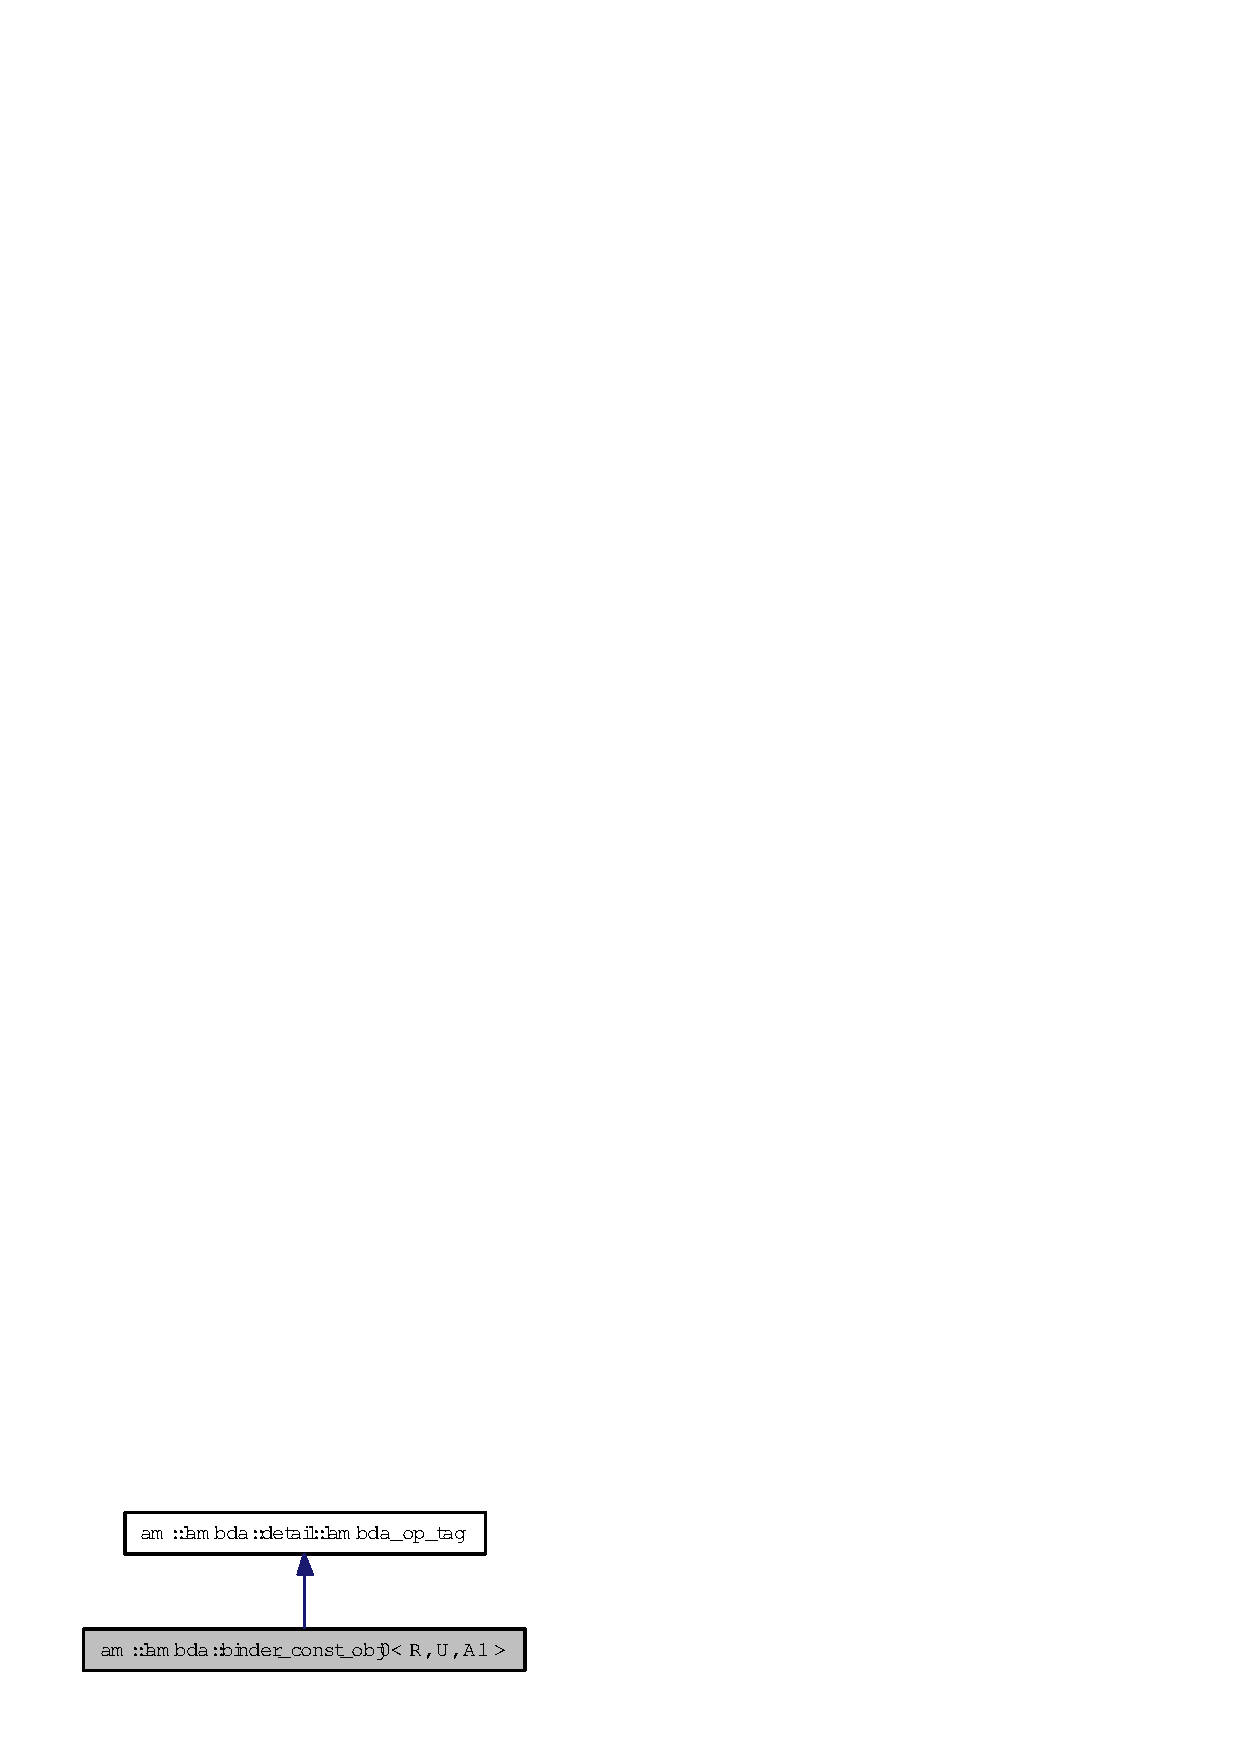
\includegraphics[width=128pt]{structam_1_1lambda_1_1binder__const__obj0__inherit__graph}
\end{center}
\end{figure}
Collaboration diagram for am::lambda::binder\_\-const\_\-obj0$<$ R, U, A1 $>$:\begin{figure}[H]
\begin{center}
\leavevmode
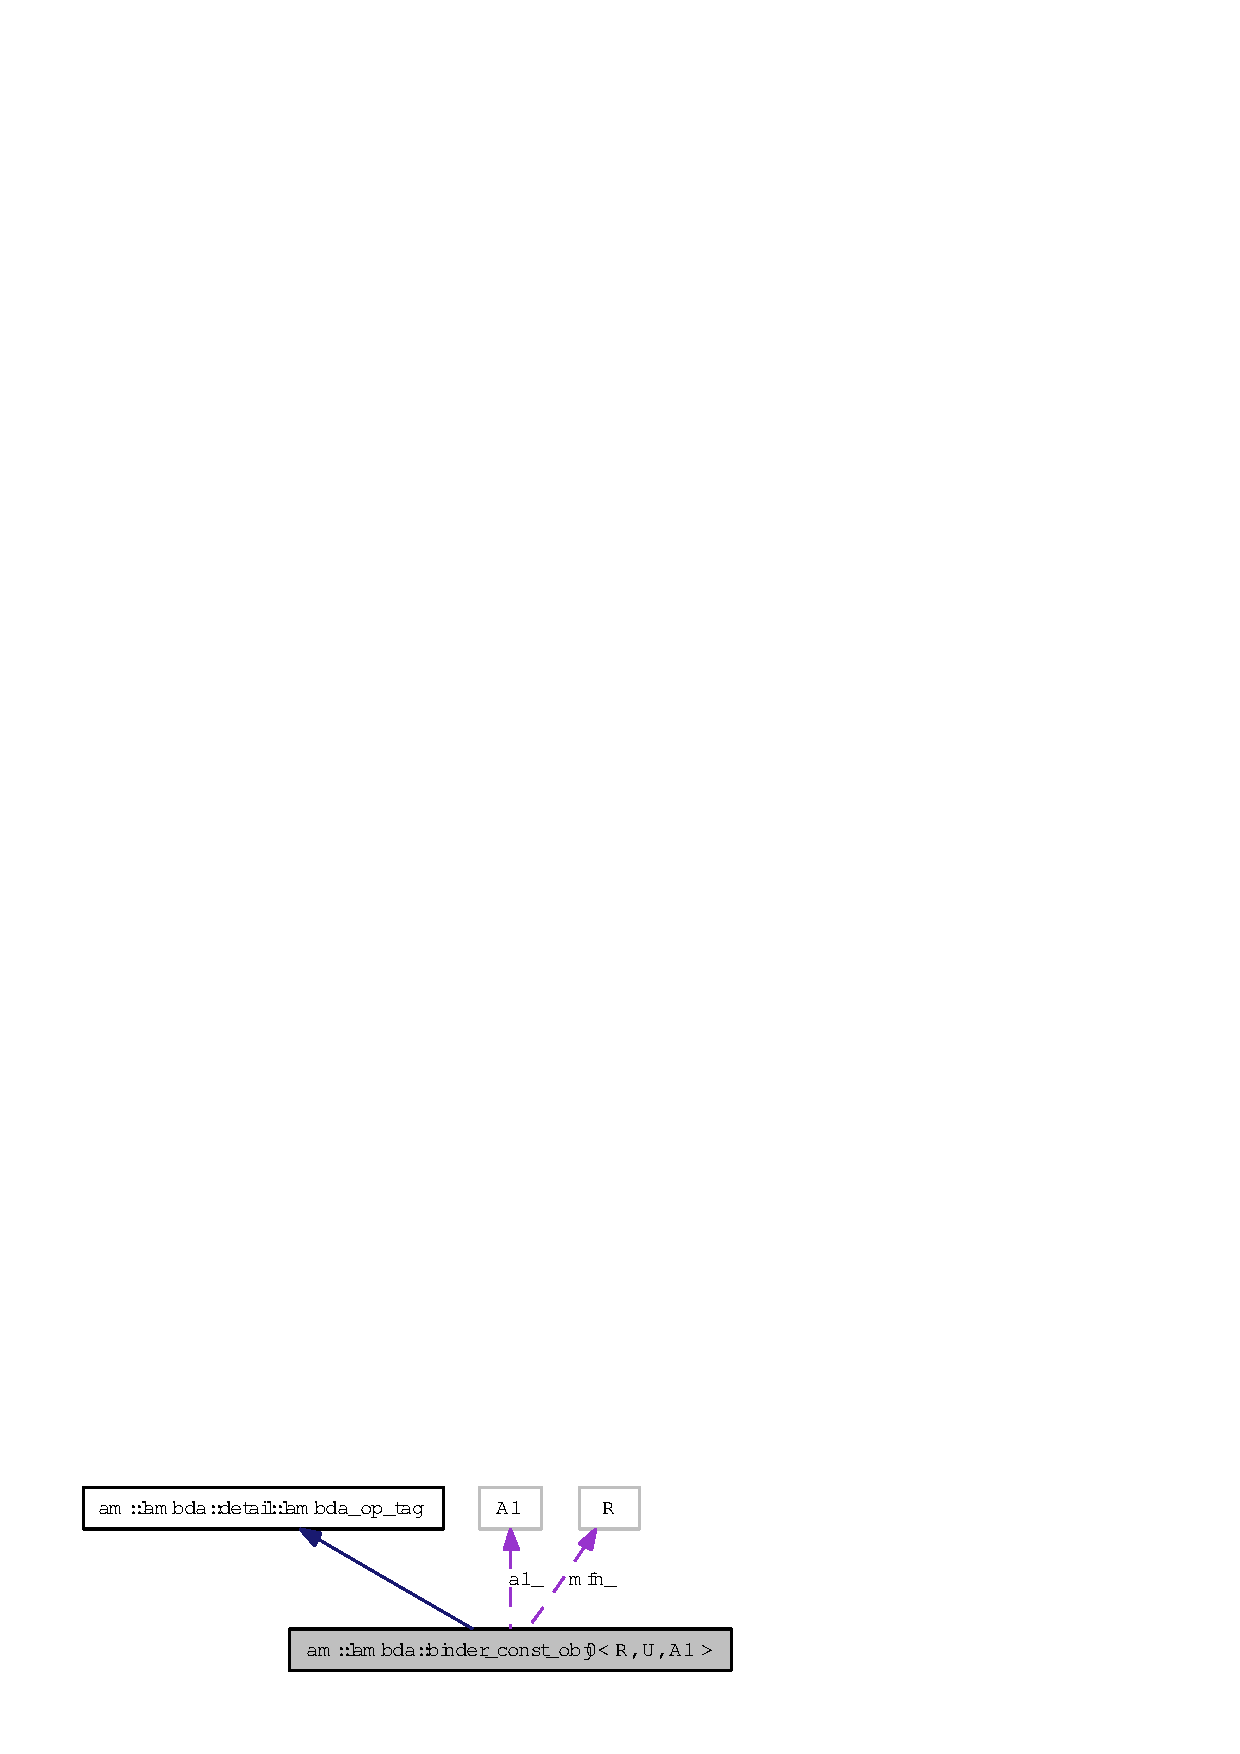
\includegraphics[width=177pt]{structam_1_1lambda_1_1binder__const__obj0__coll__graph}
\end{center}
\end{figure}
\subsection*{Public Types}
\begin{CompactItemize}
\item 
typedef detail::binder\_\-impl$<$ R $>$::result\_\-type \textbf{result\_\-type}\label{structam_1_1lambda_1_1binder__const__obj0_055117c27ab8352ae0e6e776b59745bd}

\end{CompactItemize}
\subsection*{Public Member Functions}
\begin{CompactItemize}
\item 
\textbf{binder\_\-const\_\-obj0} (R(U::$\ast$mfn)() const, A1 a1)\label{structam_1_1lambda_1_1binder__const__obj0_9b3f2e787da9f85bd99ff36e10cdbe10}

\item 
template$<$class T1, class T2, class T3$>$ result\_\-type \textbf{operator()} (T1 t1, T2 t2, T3 t3) const \label{structam_1_1lambda_1_1binder__const__obj0_a8658166542e56fa40645d7ae7ada3e0}

\item 
template$<$class T1, class T2$>$ result\_\-type \textbf{operator()} (T1 t1, T2 t2) const\label{structam_1_1lambda_1_1binder__const__obj0_47d6a0211959332726d12a7790921a3f}

\item 
template$<$class T1$>$ result\_\-type \textbf{operator()} (T1 t1) const \label{structam_1_1lambda_1_1binder__const__obj0_824a51c217745d5ce0ba139749025861}

\item 
result\_\-type \textbf{operator()} () const\label{structam_1_1lambda_1_1binder__const__obj0_cca85eae6079b261eec439d2911f59c3}

\end{CompactItemize}
\subsection*{Public Attributes}
\begin{CompactItemize}
\item 
R(U::$\ast$ \textbf{mfn\_\-} )() const\label{structam_1_1lambda_1_1binder__const__obj0_2fb09560f852e16a7d654ef63091aff0}

\item 
A1 \textbf{a1\_\-}\label{structam_1_1lambda_1_1binder__const__obj0_b46685b5ad8a378c0e8b125eff4122ad}

\end{CompactItemize}


\subsection{Detailed Description}
\subsubsection*{template$<$typename R, typename U, typename A1$>$ struct am::lambda::binder\_\-const\_\-obj0$<$ R, U, A1 $>$}

Binder for the const member function which takes the first argument as object on which the member function is being called and no extra arugement. 



The documentation for this struct was generated from the following file:\begin{CompactItemize}
\item 
{\bf lambda.hpp}\end{CompactItemize}

\section{am::lambda::binder\_\-const\_\-obj1$<$ R, P1, U, A1, A2 $>$ Struct Template Reference}
\label{structam_1_1lambda_1_1binder__const__obj1}\index{am::lambda::binder_const_obj1@{am::lambda::binder\_\-const\_\-obj1}}
{\tt \#include $<$lambda.hpp$>$}

Inherits {\bf am::lambda::detail::lambda\_\-op\_\-tag}.

Inheritance diagram for am::lambda::binder\_\-const\_\-obj1$<$ R, P1, U, A1, A2 $>$:\begin{figure}[H]
\begin{center}
\leavevmode
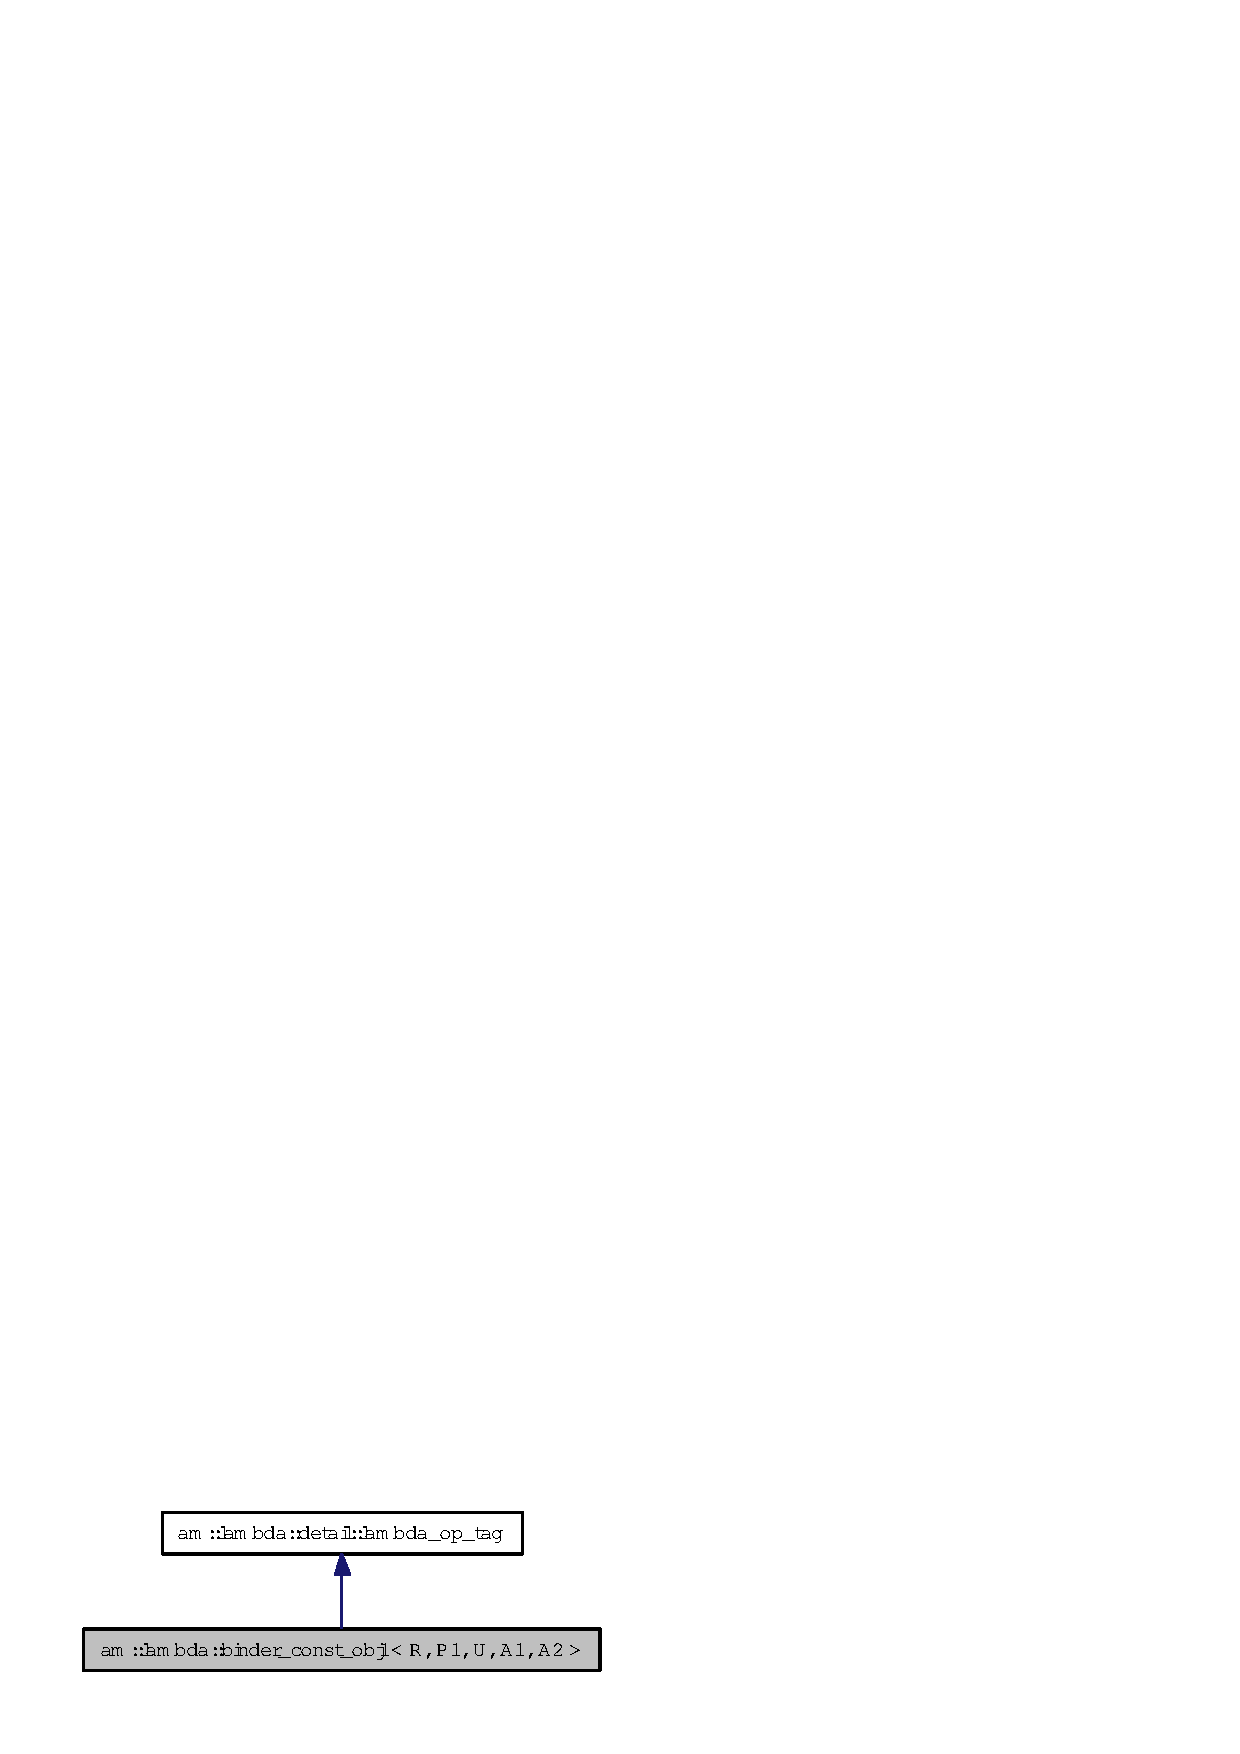
\includegraphics[width=146pt]{structam_1_1lambda_1_1binder__const__obj1__inherit__graph}
\end{center}
\end{figure}
Collaboration diagram for am::lambda::binder\_\-const\_\-obj1$<$ R, P1, U, A1, A2 $>$:\begin{figure}[H]
\begin{center}
\leavevmode
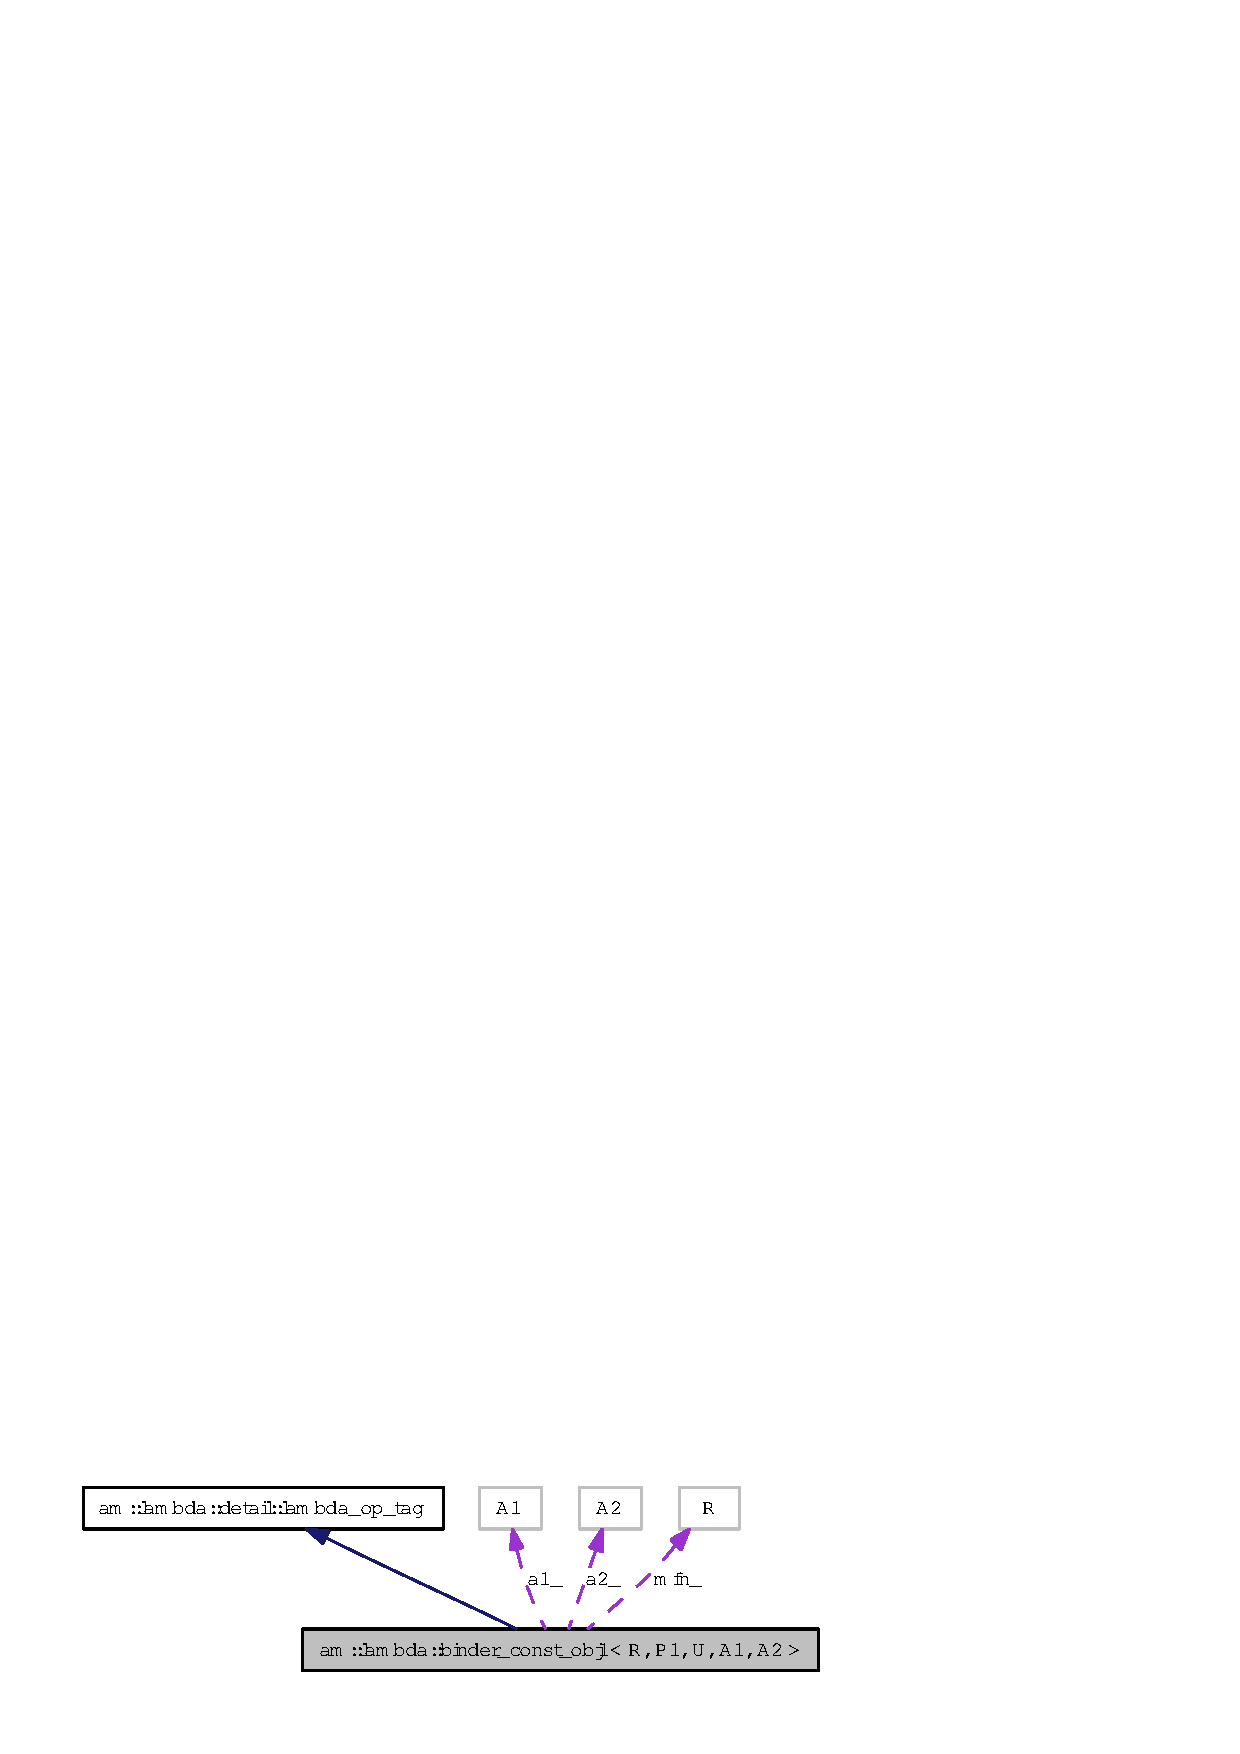
\includegraphics[width=198pt]{structam_1_1lambda_1_1binder__const__obj1__coll__graph}
\end{center}
\end{figure}
\subsection*{Public Types}
\begin{CompactItemize}
\item 
typedef detail::binder\_\-impl$<$ R $>$::result\_\-type \textbf{result\_\-type}\label{structam_1_1lambda_1_1binder__const__obj1_2e28710b27809b1164ec8049296c83b1}

\end{CompactItemize}
\subsection*{Public Member Functions}
\begin{CompactItemize}
\item 
\textbf{binder\_\-const\_\-obj1} (R(U::$\ast$mfn)(P1) const, A1 a1, A2 a2)\label{structam_1_1lambda_1_1binder__const__obj1_47feeaff4557f1447b3cdf4321e711d6}

\item 
template$<$class T1, class T2, class T3$>$ result\_\-type \textbf{operator()} (T1 t1, T2 t2, T3 t3) const \label{structam_1_1lambda_1_1binder__const__obj1_bdf91b1530eef1ae77363f1f0bf6611d}

\item 
template$<$class T1, class T2$>$ result\_\-type \textbf{operator()} (T1 t1, T2 t2) const\label{structam_1_1lambda_1_1binder__const__obj1_f956f6211d0e4b671a8da274fec1856b}

\item 
template$<$class T1$>$ result\_\-type \textbf{operator()} (T1 t1) const \label{structam_1_1lambda_1_1binder__const__obj1_d0454dd843d61eb2bd07ead76866e9ab}

\item 
result\_\-type \textbf{operator()} () const\label{structam_1_1lambda_1_1binder__const__obj1_04ad7a0a0b5403a039a855ef06daac01}

\end{CompactItemize}
\subsection*{Public Attributes}
\begin{CompactItemize}
\item 
R(U::$\ast$ \textbf{mfn\_\-} )(P1) const\label{structam_1_1lambda_1_1binder__const__obj1_ac9115fc1d2339910f7af5d3614b03f9}

\item 
A1 \textbf{a1\_\-}\label{structam_1_1lambda_1_1binder__const__obj1_fff32d21d2458b5c998e4c5e8ddc608d}

\item 
A2 \textbf{a2\_\-}\label{structam_1_1lambda_1_1binder__const__obj1_715b4504a65b59d36f9d2663a0f6d270}

\end{CompactItemize}


\subsection{Detailed Description}
\subsubsection*{template$<$typename R, typename P1, typename U, typename A1, typename A2$>$ struct am::lambda::binder\_\-const\_\-obj1$<$ R, P1, U, A1, A2 $>$}

Binder for the const member function which takes the first argument as object on which the member function is being called and one more argument. 



The documentation for this struct was generated from the following file:\begin{CompactItemize}
\item 
{\bf lambda.hpp}\end{CompactItemize}

\section{am::lambda::binder\_\-const\_\-obj2$<$ R, P1, P2, U, A1, A2, A3 $>$ Struct Template Reference}
\label{structam_1_1lambda_1_1binder__const__obj2}\index{am::lambda::binder_const_obj2@{am::lambda::binder\_\-const\_\-obj2}}
{\tt \#include $<$lambda.hpp$>$}

Inherits {\bf am::lambda::detail::lambda\_\-op\_\-tag}.

Inheritance diagram for am::lambda::binder\_\-const\_\-obj2$<$ R, P1, P2, U, A1, A2, A3 $>$:\begin{figure}[H]
\begin{center}
\leavevmode
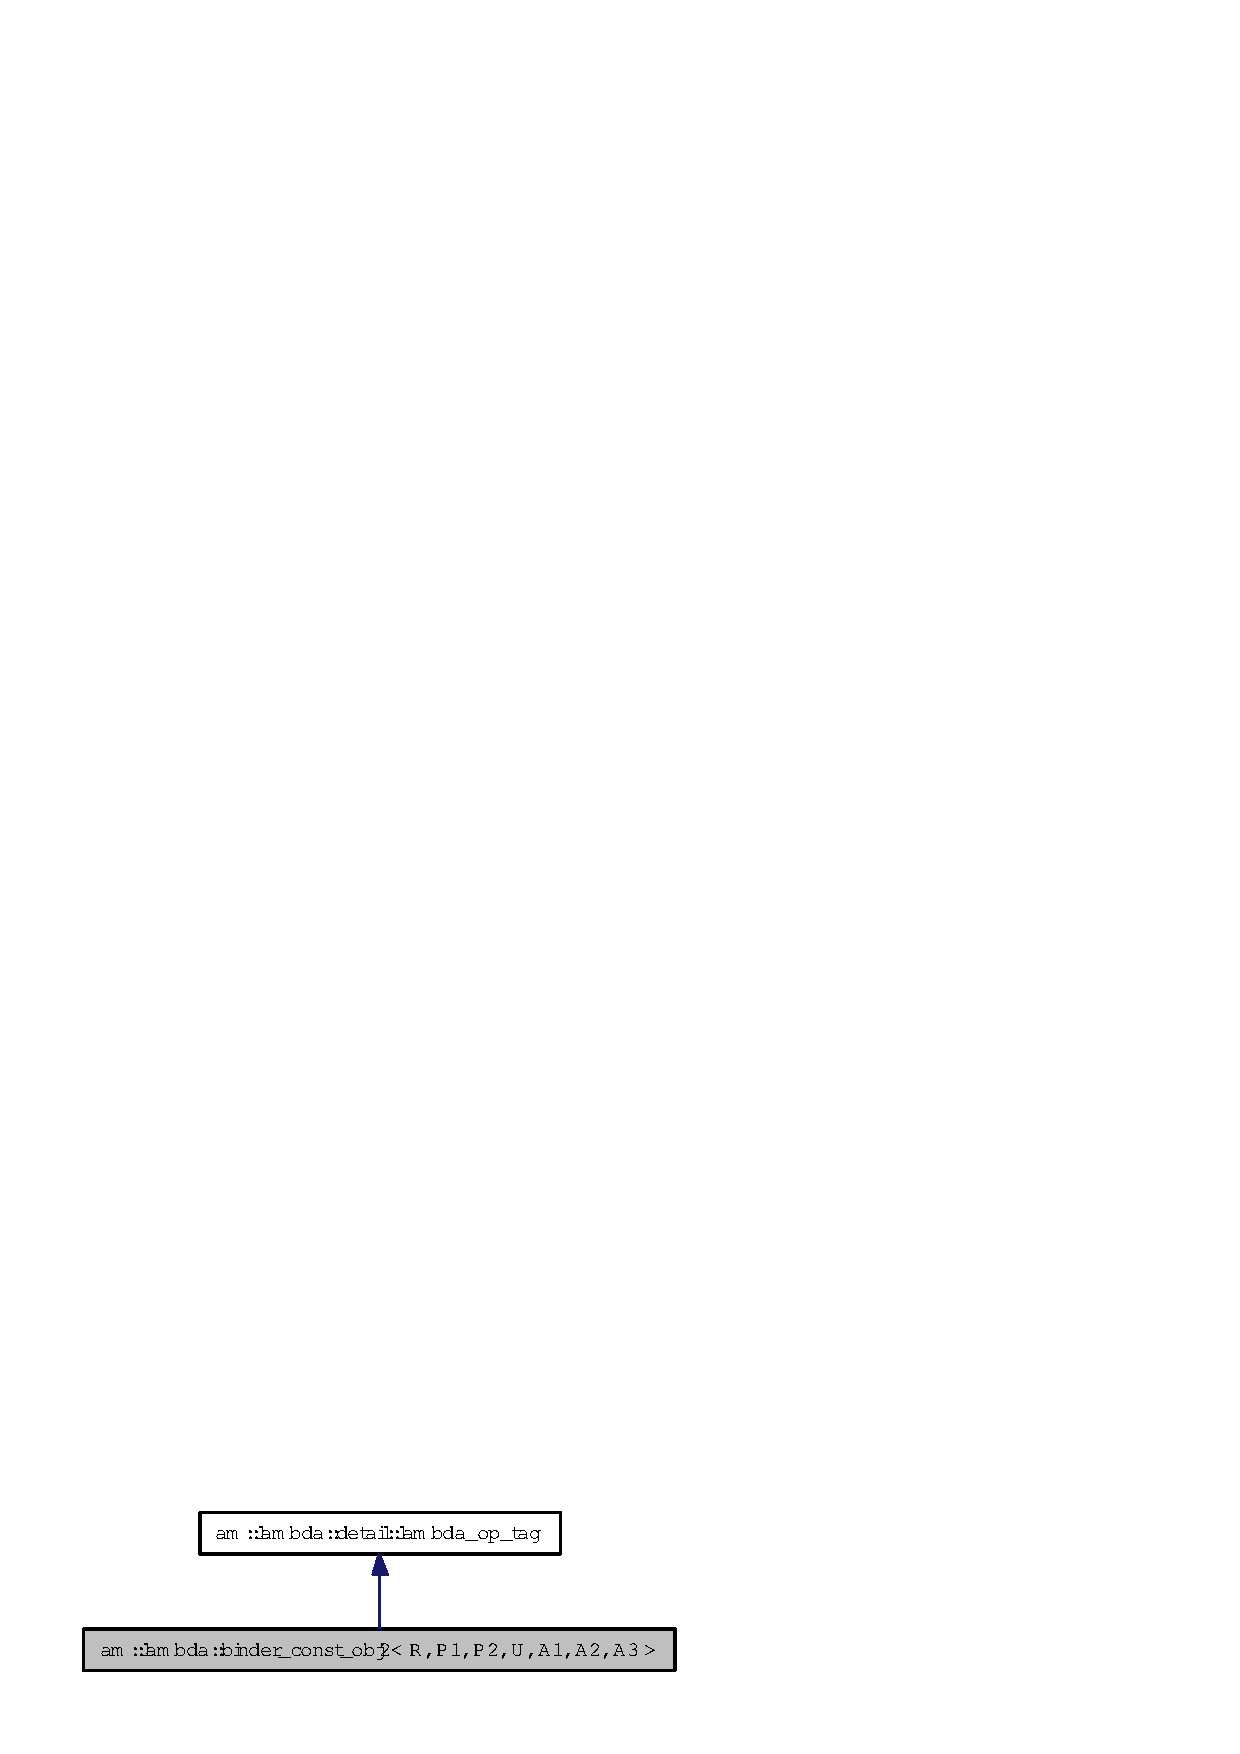
\includegraphics[width=164pt]{structam_1_1lambda_1_1binder__const__obj2__inherit__graph}
\end{center}
\end{figure}
Collaboration diagram for am::lambda::binder\_\-const\_\-obj2$<$ R, P1, P2, U, A1, A2, A3 $>$:\begin{figure}[H]
\begin{center}
\leavevmode
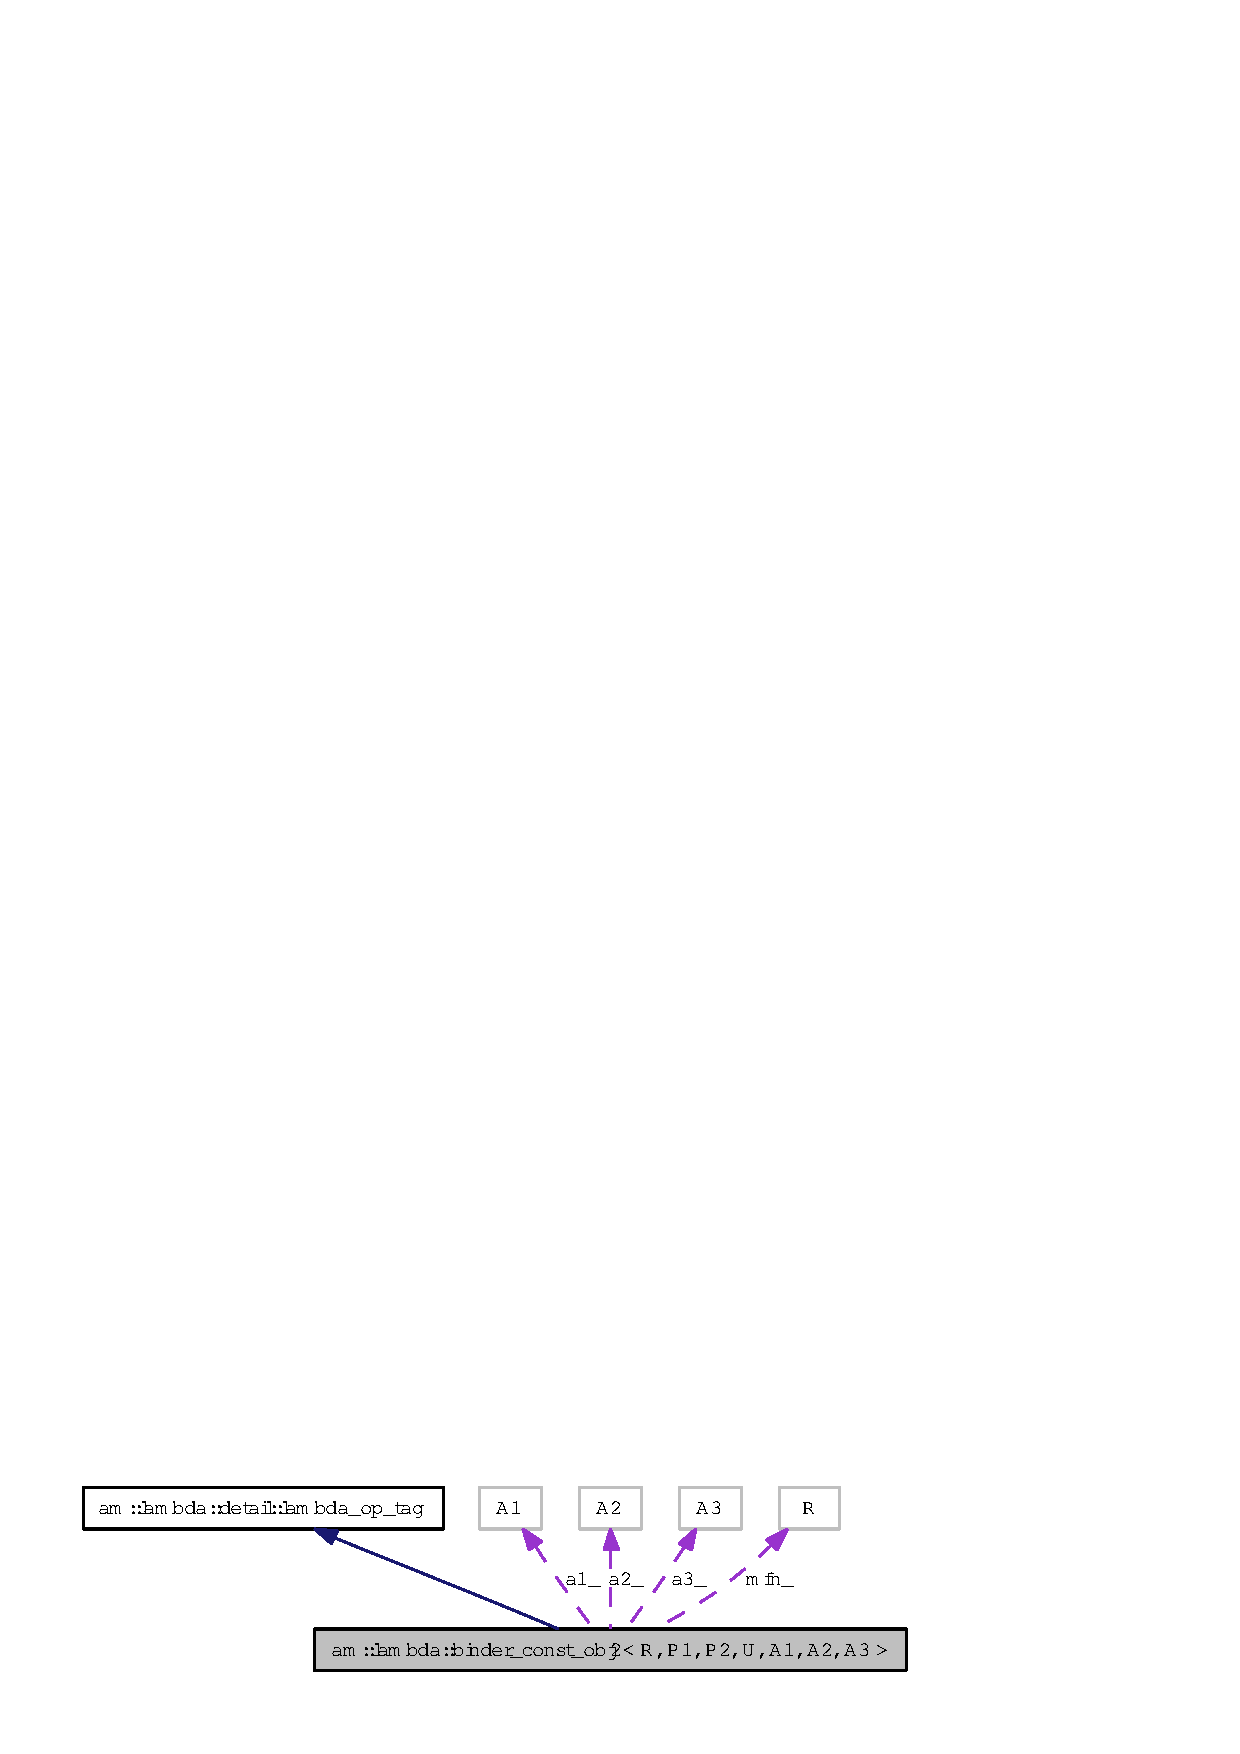
\includegraphics[width=219pt]{structam_1_1lambda_1_1binder__const__obj2__coll__graph}
\end{center}
\end{figure}
\subsection*{Public Types}
\begin{CompactItemize}
\item 
typedef detail::binder\_\-impl$<$ R $>$::result\_\-type \textbf{result\_\-type}\label{structam_1_1lambda_1_1binder__const__obj2_7115a7cf5632ba71ff68c294f4509c7b}

\end{CompactItemize}
\subsection*{Public Member Functions}
\begin{CompactItemize}
\item 
\textbf{binder\_\-const\_\-obj2} (R(U::$\ast$mfn)(P1, P2) const, A1 a1, A2 a2, A3 a3)\label{structam_1_1lambda_1_1binder__const__obj2_9873ba12fed8a7412dee117b234d2e33}

\item 
template$<$class T1, class T2, class T3$>$ result\_\-type \textbf{operator()} (T1 t1, T2 t2, T3 t3) const \label{structam_1_1lambda_1_1binder__const__obj2_c3aef6197d7630ada5709194e1aaae20}

\item 
template$<$class T1, class T2$>$ result\_\-type \textbf{operator()} (T1 t1, T2 t2) const\label{structam_1_1lambda_1_1binder__const__obj2_f90471594a26cfbb747852ddd35e3ea6}

\item 
template$<$class T1$>$ result\_\-type \textbf{operator()} (T1 t1) const \label{structam_1_1lambda_1_1binder__const__obj2_bf2325d018c31f355e17c131fe34ab9e}

\item 
result\_\-type \textbf{operator()} () const\label{structam_1_1lambda_1_1binder__const__obj2_a4135f68ee3bf490d60971dda56b63a7}

\end{CompactItemize}
\subsection*{Public Attributes}
\begin{CompactItemize}
\item 
R(U::$\ast$ \textbf{mfn\_\-} )(P1, P2) const\label{structam_1_1lambda_1_1binder__const__obj2_ef7bf0d78820f6e964887b1c2eab8f32}

\item 
A1 \textbf{a1\_\-}\label{structam_1_1lambda_1_1binder__const__obj2_6a8fbc8d0f93122d2c75d706b9353a95}

\item 
A2 \textbf{a2\_\-}\label{structam_1_1lambda_1_1binder__const__obj2_42ec377b810e7207534cd56d7de2a29c}

\item 
A3 \textbf{a3\_\-}\label{structam_1_1lambda_1_1binder__const__obj2_e995b5c44db3117ea27dc3a7393236e7}

\end{CompactItemize}


\subsection{Detailed Description}
\subsubsection*{template$<$typename R, typename P1, typename P2, typename U, typename A1, typename A2, typename A3$>$ struct am::lambda::binder\_\-const\_\-obj2$<$ R, P1, P2, U, A1, A2, A3 $>$}

Binder for the const member function which takes the first argument as object on which the member function is being called and two more arguments. 



The documentation for this struct was generated from the following file:\begin{CompactItemize}
\item 
{\bf lambda.hpp}\end{CompactItemize}

\section{am::lambda::binder\_\-const\_\-obj3$<$ R, P1, P2, P3, U, A1, A2, A3, A4 $>$ Struct Template Reference}
\label{structam_1_1lambda_1_1binder__const__obj3}\index{am::lambda::binder_const_obj3@{am::lambda::binder\_\-const\_\-obj3}}
{\tt \#include $<$lambda.hpp$>$}

Inherits {\bf am::lambda::detail::lambda\_\-op\_\-tag}.

Inheritance diagram for am::lambda::binder\_\-const\_\-obj3$<$ R, P1, P2, P3, U, A1, A2, A3, A4 $>$:\begin{figure}[H]
\begin{center}
\leavevmode
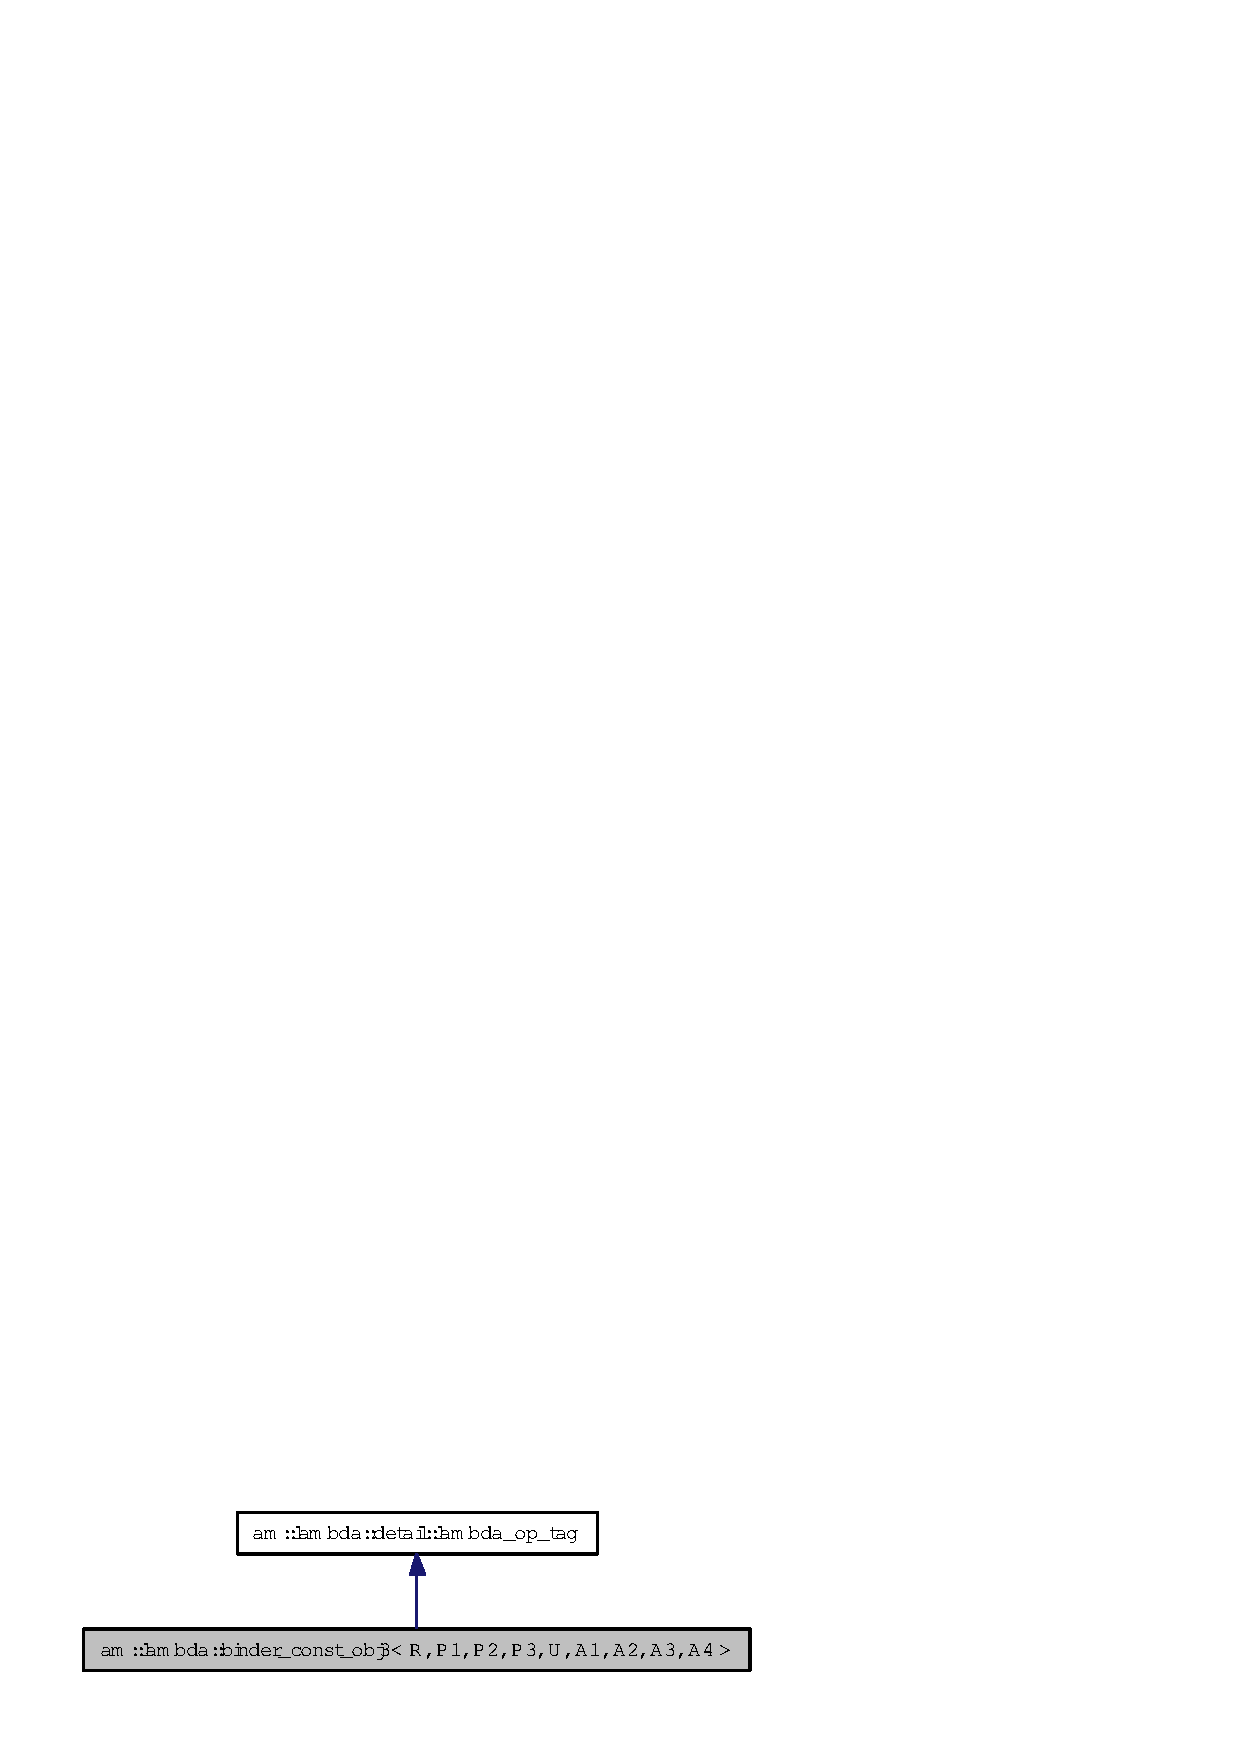
\includegraphics[width=182pt]{structam_1_1lambda_1_1binder__const__obj3__inherit__graph}
\end{center}
\end{figure}
Collaboration diagram for am::lambda::binder\_\-const\_\-obj3$<$ R, P1, P2, P3, U, A1, A2, A3, A4 $>$:\begin{figure}[H]
\begin{center}
\leavevmode
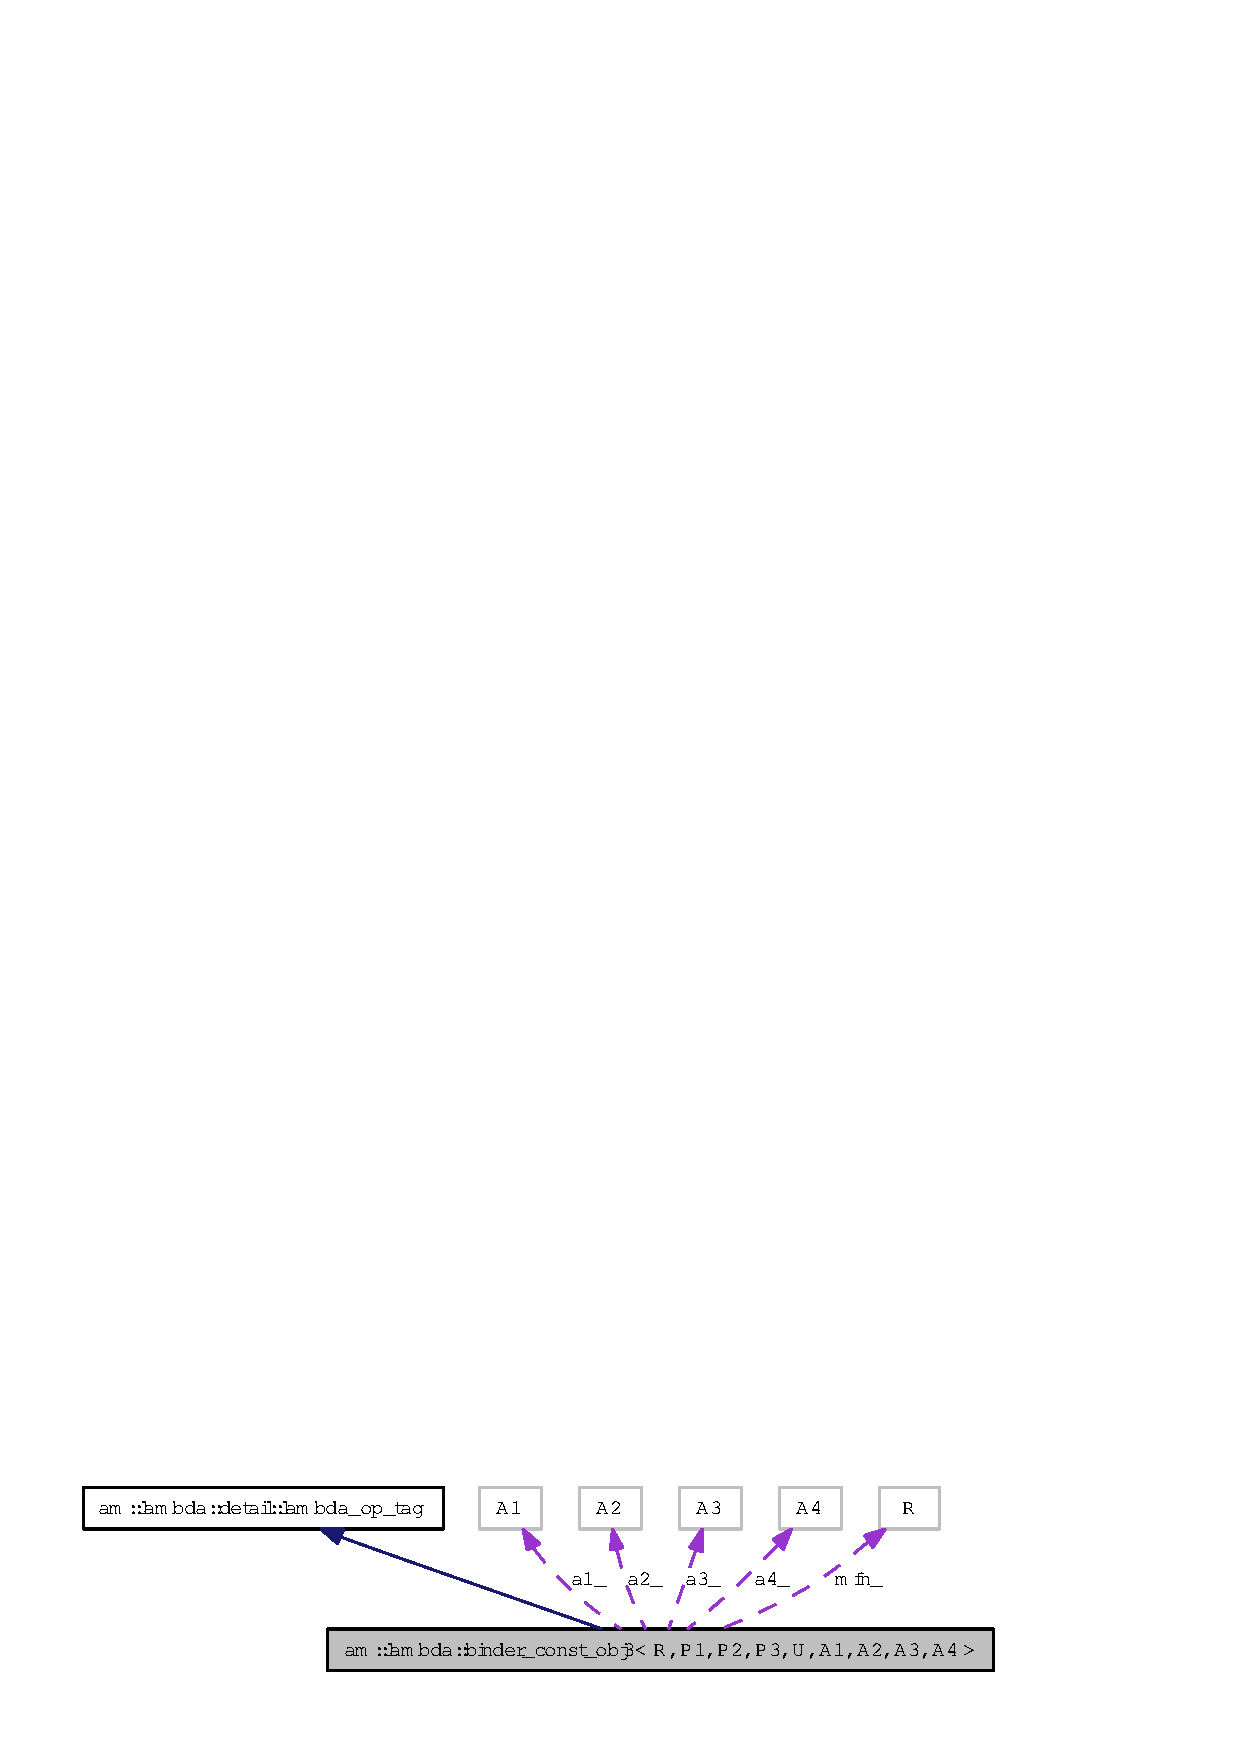
\includegraphics[width=240pt]{structam_1_1lambda_1_1binder__const__obj3__coll__graph}
\end{center}
\end{figure}
\subsection*{Public Types}
\begin{CompactItemize}
\item 
typedef detail::binder\_\-impl$<$ R $>$::result\_\-type \textbf{result\_\-type}\label{structam_1_1lambda_1_1binder__const__obj3_d81d5d7d42c92cc8cccdcb8e66f75d5f}

\end{CompactItemize}
\subsection*{Public Member Functions}
\begin{CompactItemize}
\item 
\textbf{binder\_\-const\_\-obj3} (R(U::$\ast$mfn)(P1, P2, P3) const, A1 a1, A2 a2, A3 a3, A4 a4)\label{structam_1_1lambda_1_1binder__const__obj3_d1a2a9a00c547e964bf7bd12f8455144}

\item 
template$<$class T1, class T2, class T3$>$ result\_\-type \textbf{operator()} (T1 t1, T2 t2, T3 t3) const \label{structam_1_1lambda_1_1binder__const__obj3_a0aeefbadd1813edfff4d59f211ad7eb}

\item 
template$<$class T1, class T2$>$ result\_\-type \textbf{operator()} (T1 t1, T2 t2) const\label{structam_1_1lambda_1_1binder__const__obj3_7acb9c462d4a400221b7d84b12b6200a}

\item 
template$<$class T1$>$ result\_\-type \textbf{operator()} (T1 t1) const \label{structam_1_1lambda_1_1binder__const__obj3_0ae7249718a6fdbc02b94a5088ff24b3}

\item 
result\_\-type \textbf{operator()} () const\label{structam_1_1lambda_1_1binder__const__obj3_56d1b211608b9b090ea98eb947150b26}

\end{CompactItemize}
\subsection*{Public Attributes}
\begin{CompactItemize}
\item 
R(U::$\ast$ \textbf{mfn\_\-} )(P1, P2, P3) const\label{structam_1_1lambda_1_1binder__const__obj3_deed77c1939e2e503b28abac90abf125}

\item 
A1 \textbf{a1\_\-}\label{structam_1_1lambda_1_1binder__const__obj3_bfbb7829f21725bb9cf35a060fdc46ce}

\item 
A2 \textbf{a2\_\-}\label{structam_1_1lambda_1_1binder__const__obj3_784dcc6adf943e527b9b4417769482d4}

\item 
A3 \textbf{a3\_\-}\label{structam_1_1lambda_1_1binder__const__obj3_99fd86887d6960622ef335c5cfd9466c}

\item 
A4 \textbf{a4\_\-}\label{structam_1_1lambda_1_1binder__const__obj3_9f2fe1a3562aaa1c2059e56eb8a799c6}

\end{CompactItemize}


\subsection{Detailed Description}
\subsubsection*{template$<$typename R, typename P1, typename P2, typename P3, typename U, typename A1, typename A2, typename A3, typename A4$>$ struct am::lambda::binder\_\-const\_\-obj3$<$ R, P1, P2, P3, U, A1, A2, A3, A4 $>$}

Binder for the const member function which takes the first argument as object on which the member function is being called and three more arguments. 



The documentation for this struct was generated from the following file:\begin{CompactItemize}
\item 
{\bf lambda.hpp}\end{CompactItemize}

\section{am::lambda::binder\_\-obj0$<$ R, U, A1 $>$ Struct Template Reference}
\label{structam_1_1lambda_1_1binder__obj0}\index{am::lambda::binder_obj0@{am::lambda::binder\_\-obj0}}
{\tt \#include $<$lambda.hpp$>$}

Inherits {\bf am::lambda::detail::lambda\_\-op\_\-tag}.

Inheritance diagram for am::lambda::binder\_\-obj0$<$ R, U, A1 $>$:\begin{figure}[H]
\begin{center}
\leavevmode
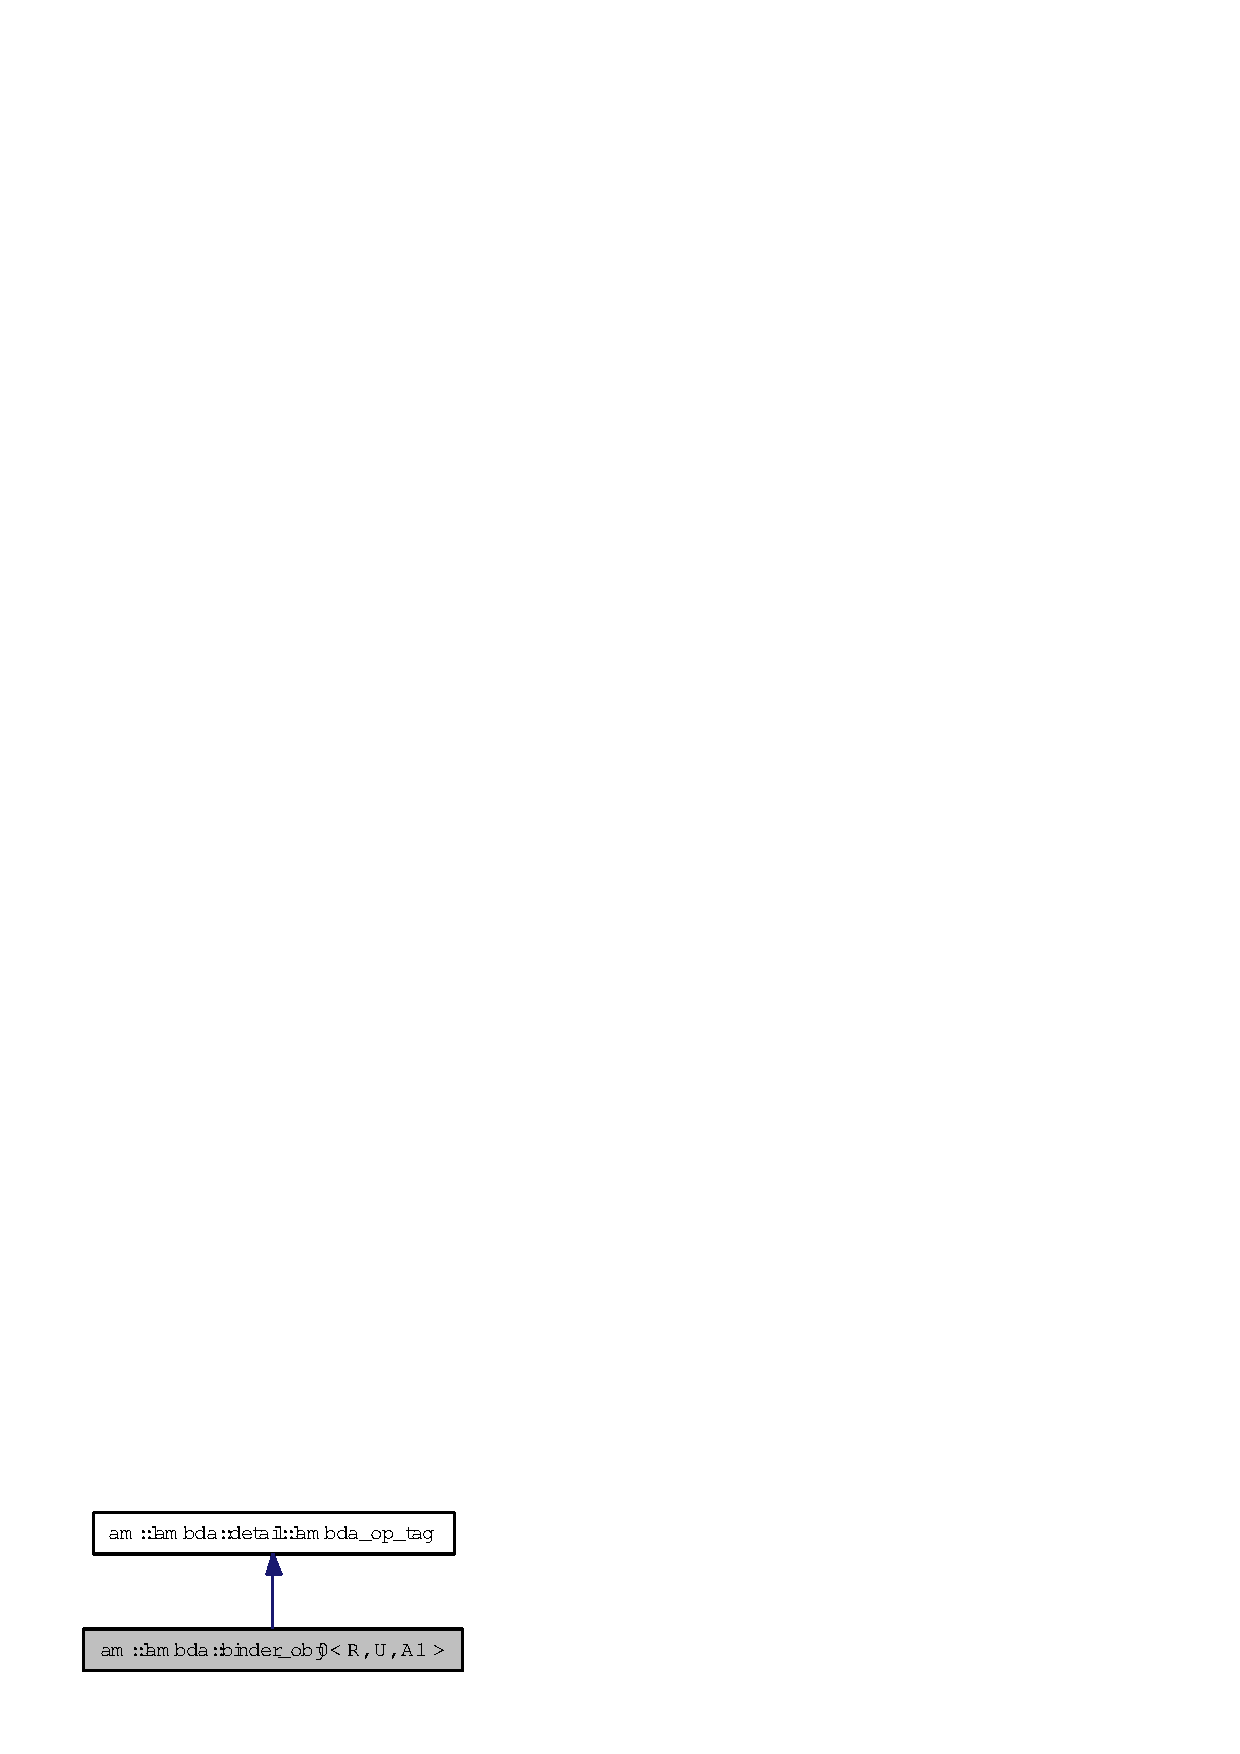
\includegraphics[width=113pt]{structam_1_1lambda_1_1binder__obj0__inherit__graph}
\end{center}
\end{figure}
Collaboration diagram for am::lambda::binder\_\-obj0$<$ R, U, A1 $>$:\begin{figure}[H]
\begin{center}
\leavevmode
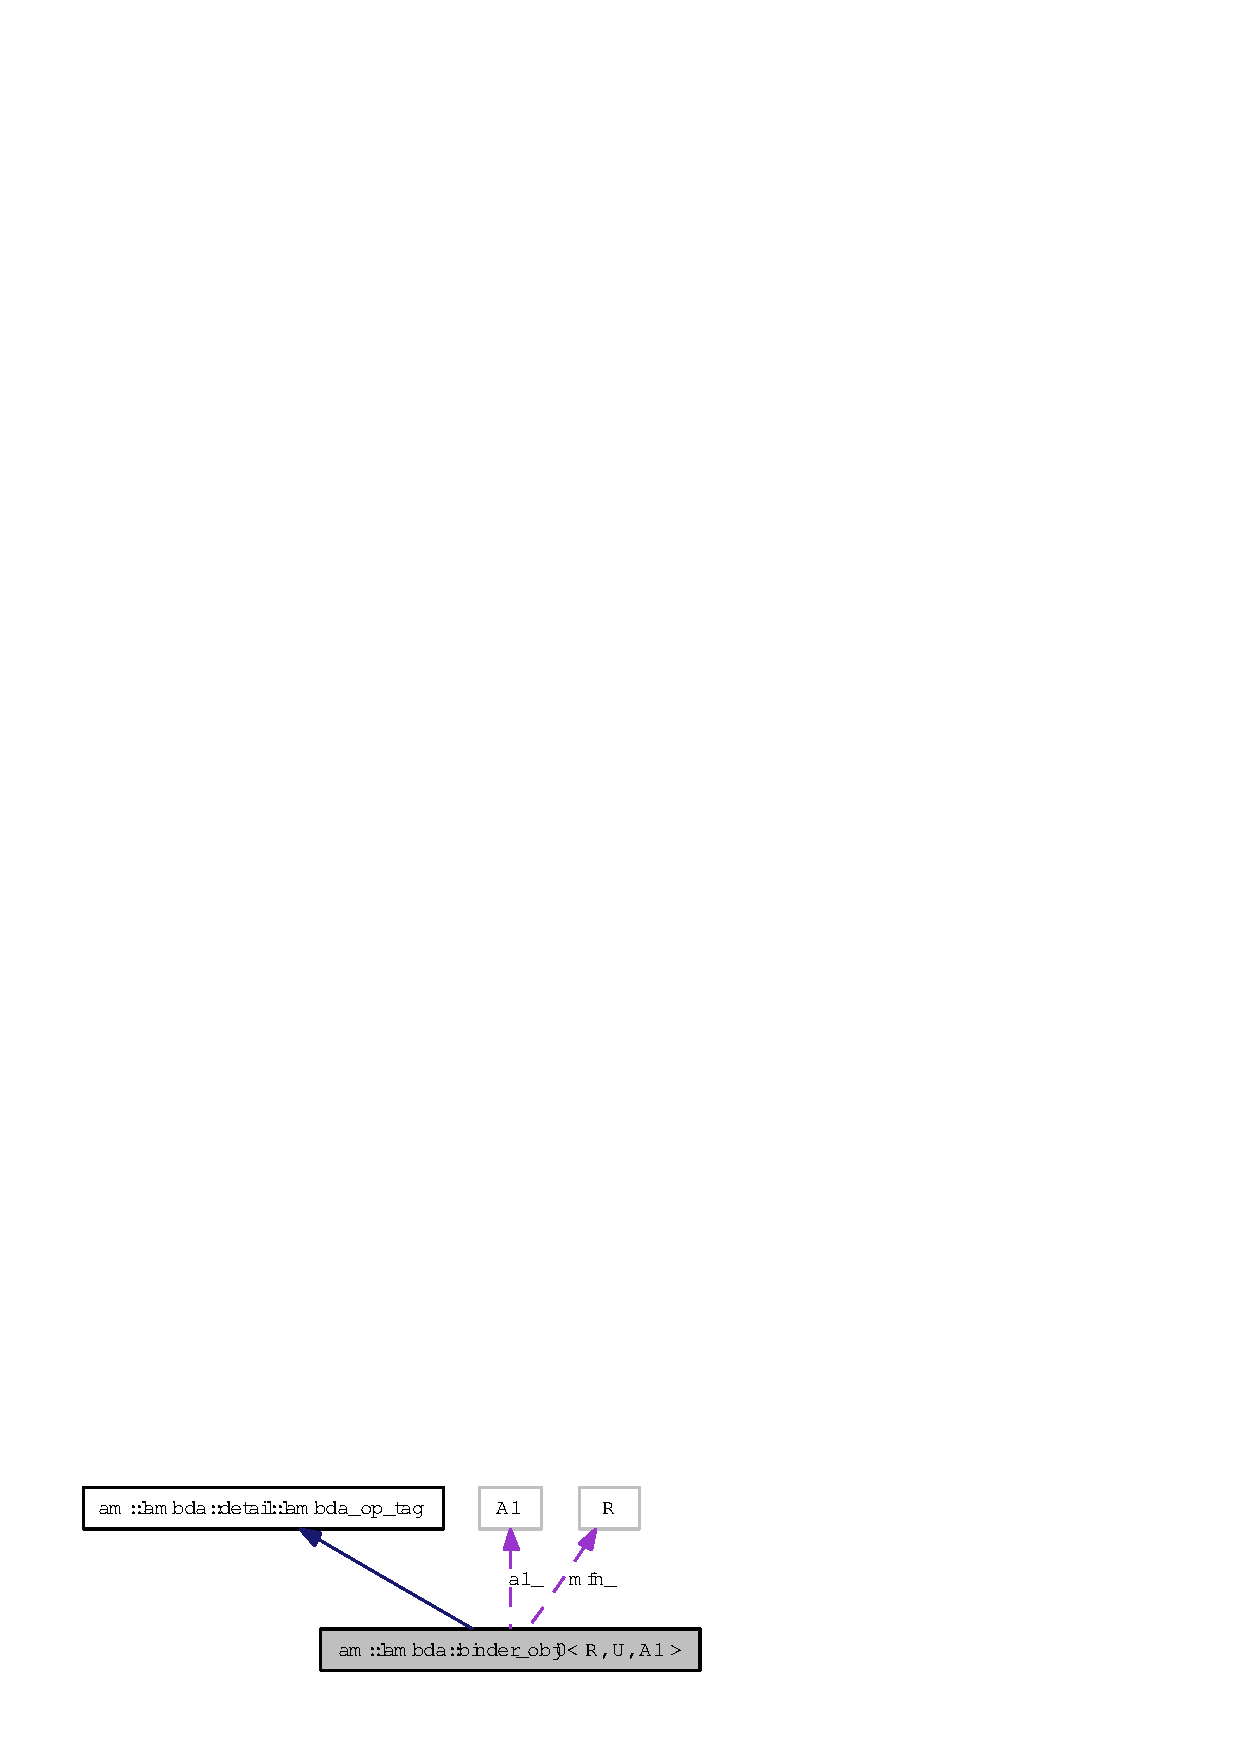
\includegraphics[width=170pt]{structam_1_1lambda_1_1binder__obj0__coll__graph}
\end{center}
\end{figure}
\subsection*{Public Types}
\begin{CompactItemize}
\item 
typedef detail::binder\_\-impl$<$ R $>$::result\_\-type \textbf{result\_\-type}\label{structam_1_1lambda_1_1binder__obj0_cb6658302f1fb19996bfbc8c3a318254}

\end{CompactItemize}
\subsection*{Public Member Functions}
\begin{CompactItemize}
\item 
\textbf{binder\_\-obj0} (R(U::$\ast$mfn)(), A1 a1)\label{structam_1_1lambda_1_1binder__obj0_5e96ad5ca1d04e03da591cdea124d409}

\item 
template$<$class T1, class T2, class T3$>$ result\_\-type \textbf{operator()} (T1 t1, T2 t2, T3 t3) const \label{structam_1_1lambda_1_1binder__obj0_a23d8ff86f058507f9af835688bc2409}

\item 
template$<$class T1, class T2$>$ result\_\-type \textbf{operator()} (T1 t1, T2 t2) const\label{structam_1_1lambda_1_1binder__obj0_a65a5695f175b8a63dcf0bb0593fb5d7}

\item 
template$<$class T1$>$ result\_\-type \textbf{operator()} (T1 t1) const \label{structam_1_1lambda_1_1binder__obj0_aa339943e2336100293ab098a837dd17}

\item 
result\_\-type \textbf{operator()} () const\label{structam_1_1lambda_1_1binder__obj0_99a0ee62fea6581e6599843168c81cb8}

\end{CompactItemize}
\subsection*{Public Attributes}
\begin{CompactItemize}
\item 
R(U::$\ast$ \textbf{mfn\_\-} )()\label{structam_1_1lambda_1_1binder__obj0_11d31750a5f862314ea7e710f4e3e06a}

\item 
A1 \textbf{a1\_\-}\label{structam_1_1lambda_1_1binder__obj0_e37004bd4caeb629f6e288f050aa67f6}

\end{CompactItemize}


\subsection{Detailed Description}
\subsubsection*{template$<$typename R, typename U, typename A1$>$ struct am::lambda::binder\_\-obj0$<$ R, U, A1 $>$}

Binder for the member function which takes the first argument as object on which the member function is being called and no extra arugement. 



The documentation for this struct was generated from the following file:\begin{CompactItemize}
\item 
{\bf lambda.hpp}\end{CompactItemize}

\section{am::lambda::binder\_\-obj1$<$ R, P1, U, A1, A2 $>$ Struct Template Reference}
\label{structam_1_1lambda_1_1binder__obj1}\index{am::lambda::binder_obj1@{am::lambda::binder\_\-obj1}}
{\tt \#include $<$lambda.hpp$>$}

Inherits {\bf am::lambda::detail::lambda\_\-op\_\-tag}.

Inheritance diagram for am::lambda::binder\_\-obj1$<$ R, P1, U, A1, A2 $>$:\begin{figure}[H]
\begin{center}
\leavevmode
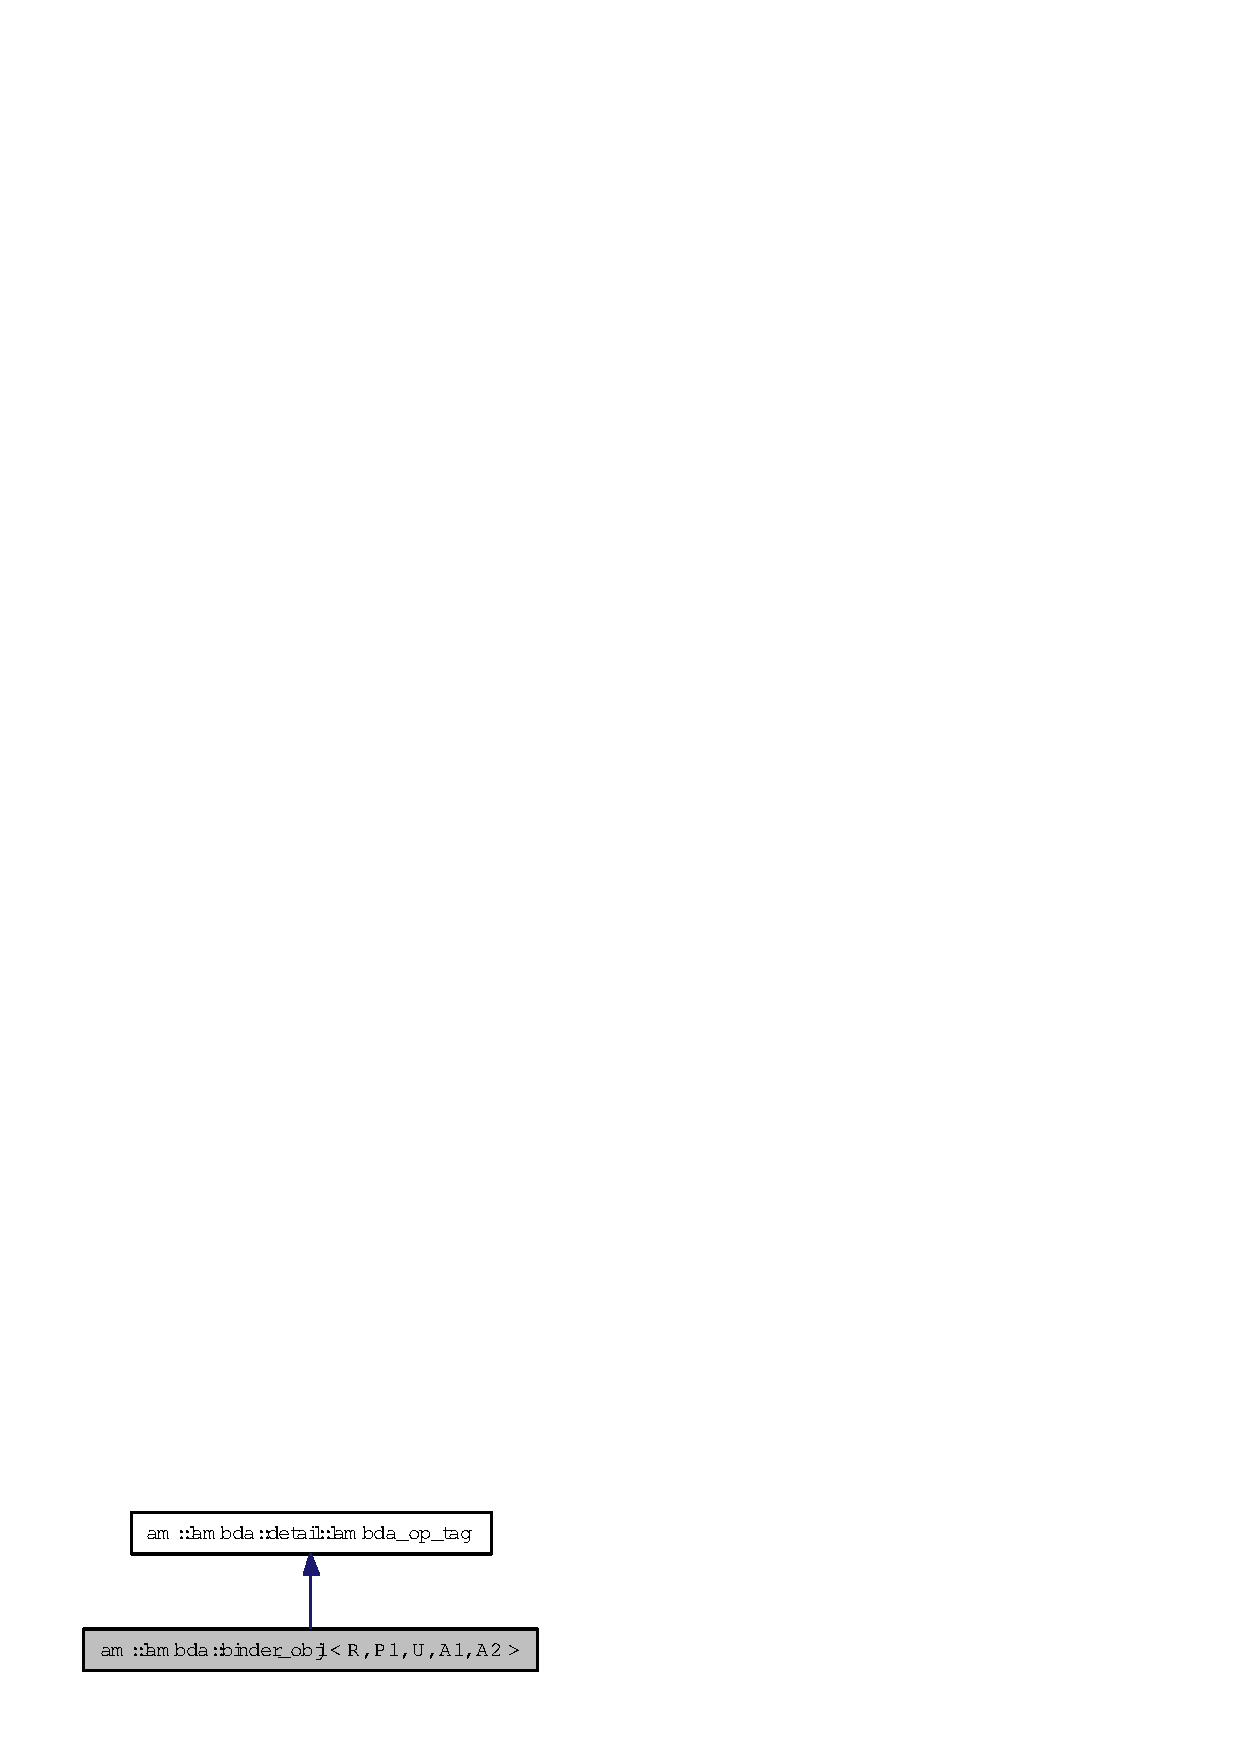
\includegraphics[width=131pt]{structam_1_1lambda_1_1binder__obj1__inherit__graph}
\end{center}
\end{figure}
Collaboration diagram for am::lambda::binder\_\-obj1$<$ R, P1, U, A1, A2 $>$:\begin{figure}[H]
\begin{center}
\leavevmode
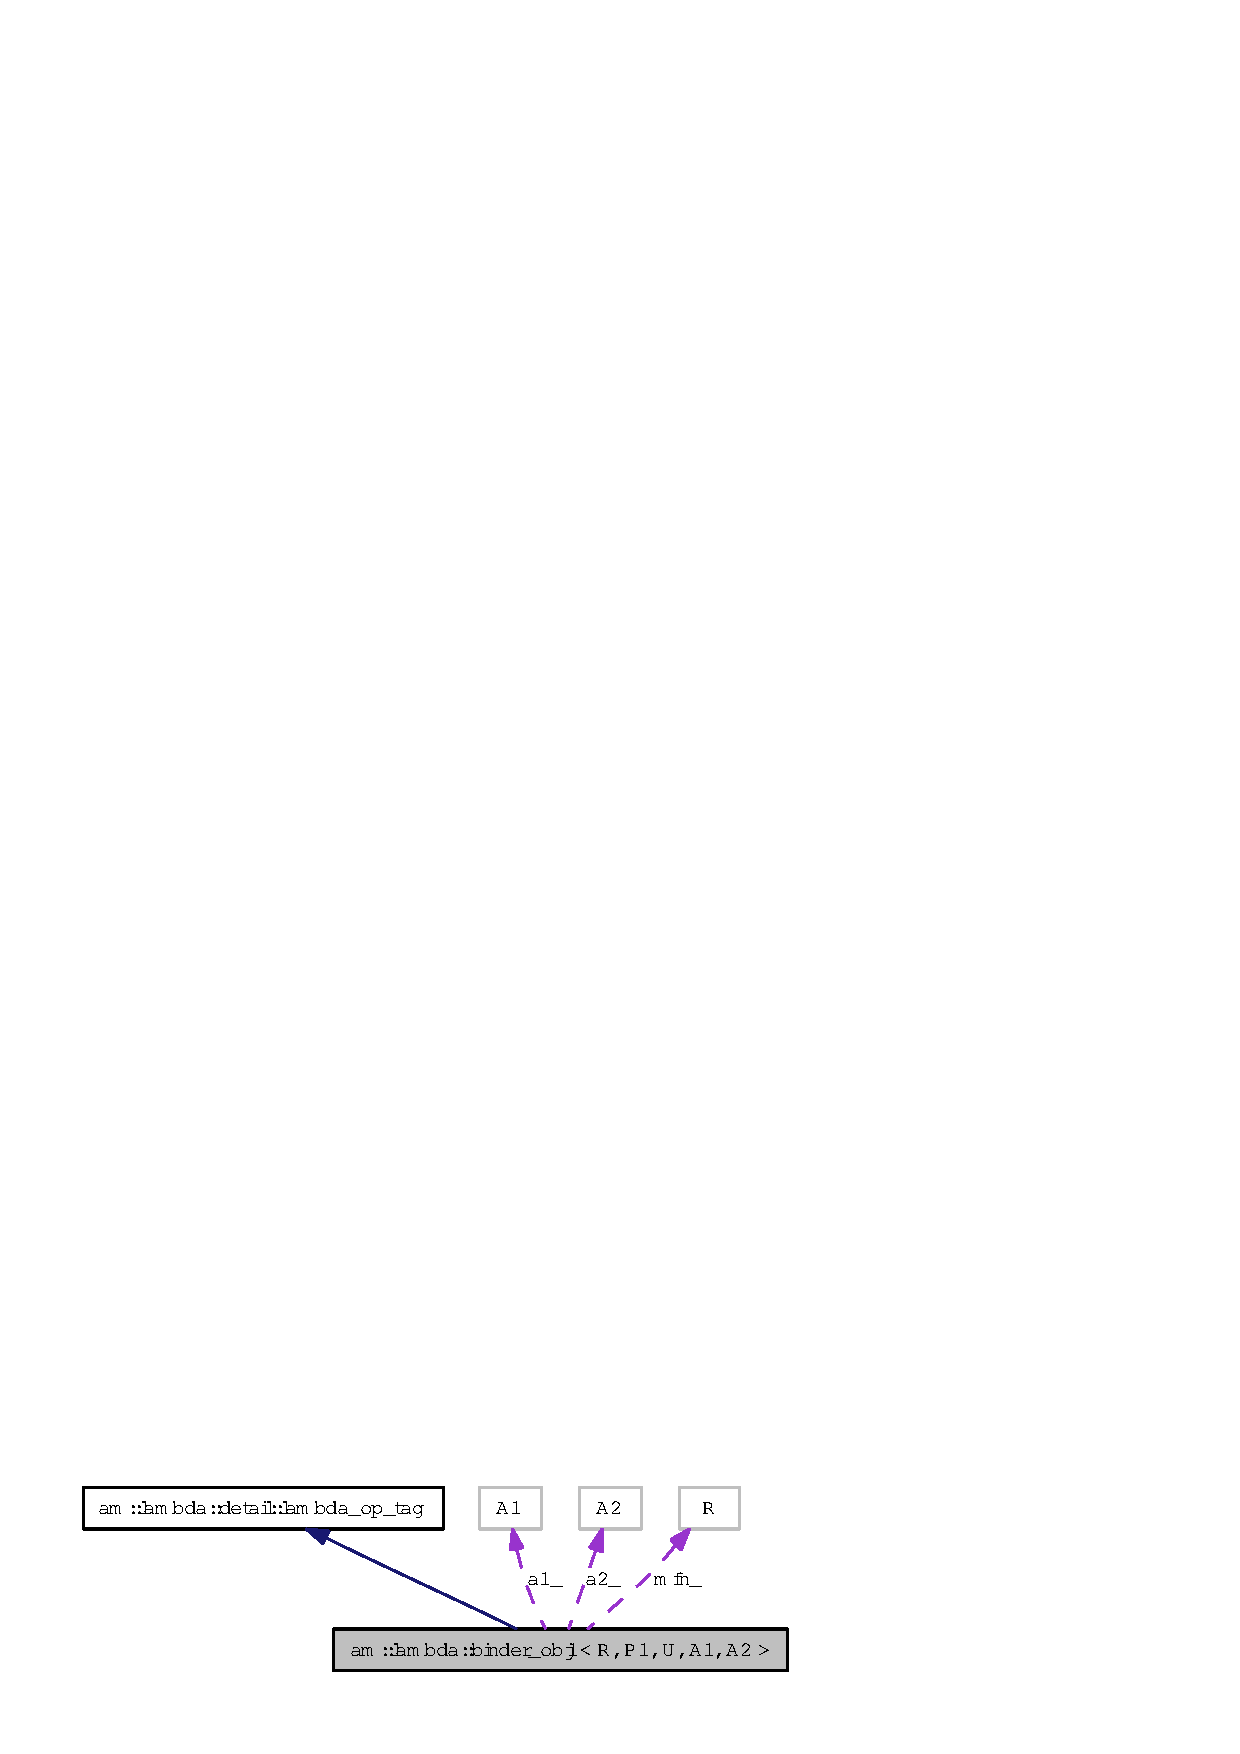
\includegraphics[width=191pt]{structam_1_1lambda_1_1binder__obj1__coll__graph}
\end{center}
\end{figure}
\subsection*{Public Types}
\begin{CompactItemize}
\item 
typedef detail::binder\_\-impl$<$ R $>$::result\_\-type \textbf{result\_\-type}\label{structam_1_1lambda_1_1binder__obj1_1a5a45d79a37b7f1df97a51134ba2578}

\end{CompactItemize}
\subsection*{Public Member Functions}
\begin{CompactItemize}
\item 
\textbf{binder\_\-obj1} (R(U::$\ast$mfn)(P1), A1 a1, A2 a2)\label{structam_1_1lambda_1_1binder__obj1_7bf6372d214724f9a9dafc24be8deaaa}

\item 
template$<$class T1, class T2, class T3$>$ result\_\-type \textbf{operator()} (T1 t1, T2 t2, T3 t3) const \label{structam_1_1lambda_1_1binder__obj1_0b3e492aeef424f851ad2dbce41a261e}

\item 
template$<$class T1, class T2$>$ result\_\-type \textbf{operator()} (T1 t1, T2 t2) const\label{structam_1_1lambda_1_1binder__obj1_3f083709255c7d1c3188d7fcaec38092}

\item 
template$<$class T1$>$ result\_\-type \textbf{operator()} (T1 t1) const \label{structam_1_1lambda_1_1binder__obj1_7bf3bcf64d9b939a666ddfe5d80183c6}

\item 
result\_\-type \textbf{operator()} () const\label{structam_1_1lambda_1_1binder__obj1_503e278a3618c3c947c4f746d411f2e9}

\end{CompactItemize}
\subsection*{Public Attributes}
\begin{CompactItemize}
\item 
R(U::$\ast$ \textbf{mfn\_\-} )(P1)\label{structam_1_1lambda_1_1binder__obj1_662b262de3c98023dfcf39536569440e}

\item 
A1 \textbf{a1\_\-}\label{structam_1_1lambda_1_1binder__obj1_a93ff0f1481333fe684726f0326fc022}

\item 
A2 \textbf{a2\_\-}\label{structam_1_1lambda_1_1binder__obj1_0cd05351917c0ecdb9126b1cbe1f1192}

\end{CompactItemize}


\subsection{Detailed Description}
\subsubsection*{template$<$typename R, typename P1, typename U, typename A1, typename A2$>$ struct am::lambda::binder\_\-obj1$<$ R, P1, U, A1, A2 $>$}

Binder for the member function which takes the first argument as object on which the member function is being called and one more argument. 



The documentation for this struct was generated from the following file:\begin{CompactItemize}
\item 
{\bf lambda.hpp}\end{CompactItemize}

\section{am::lambda::binder\_\-obj2$<$ R, P1, P2, U, A1, A2, A3 $>$ Struct Template Reference}
\label{structam_1_1lambda_1_1binder__obj2}\index{am::lambda::binder_obj2@{am::lambda::binder\_\-obj2}}
{\tt \#include $<$lambda.hpp$>$}

Inherits {\bf am::lambda::detail::lambda\_\-op\_\-tag}.

Inheritance diagram for am::lambda::binder\_\-obj2$<$ R, P1, P2, U, A1, A2, A3 $>$:\begin{figure}[H]
\begin{center}
\leavevmode
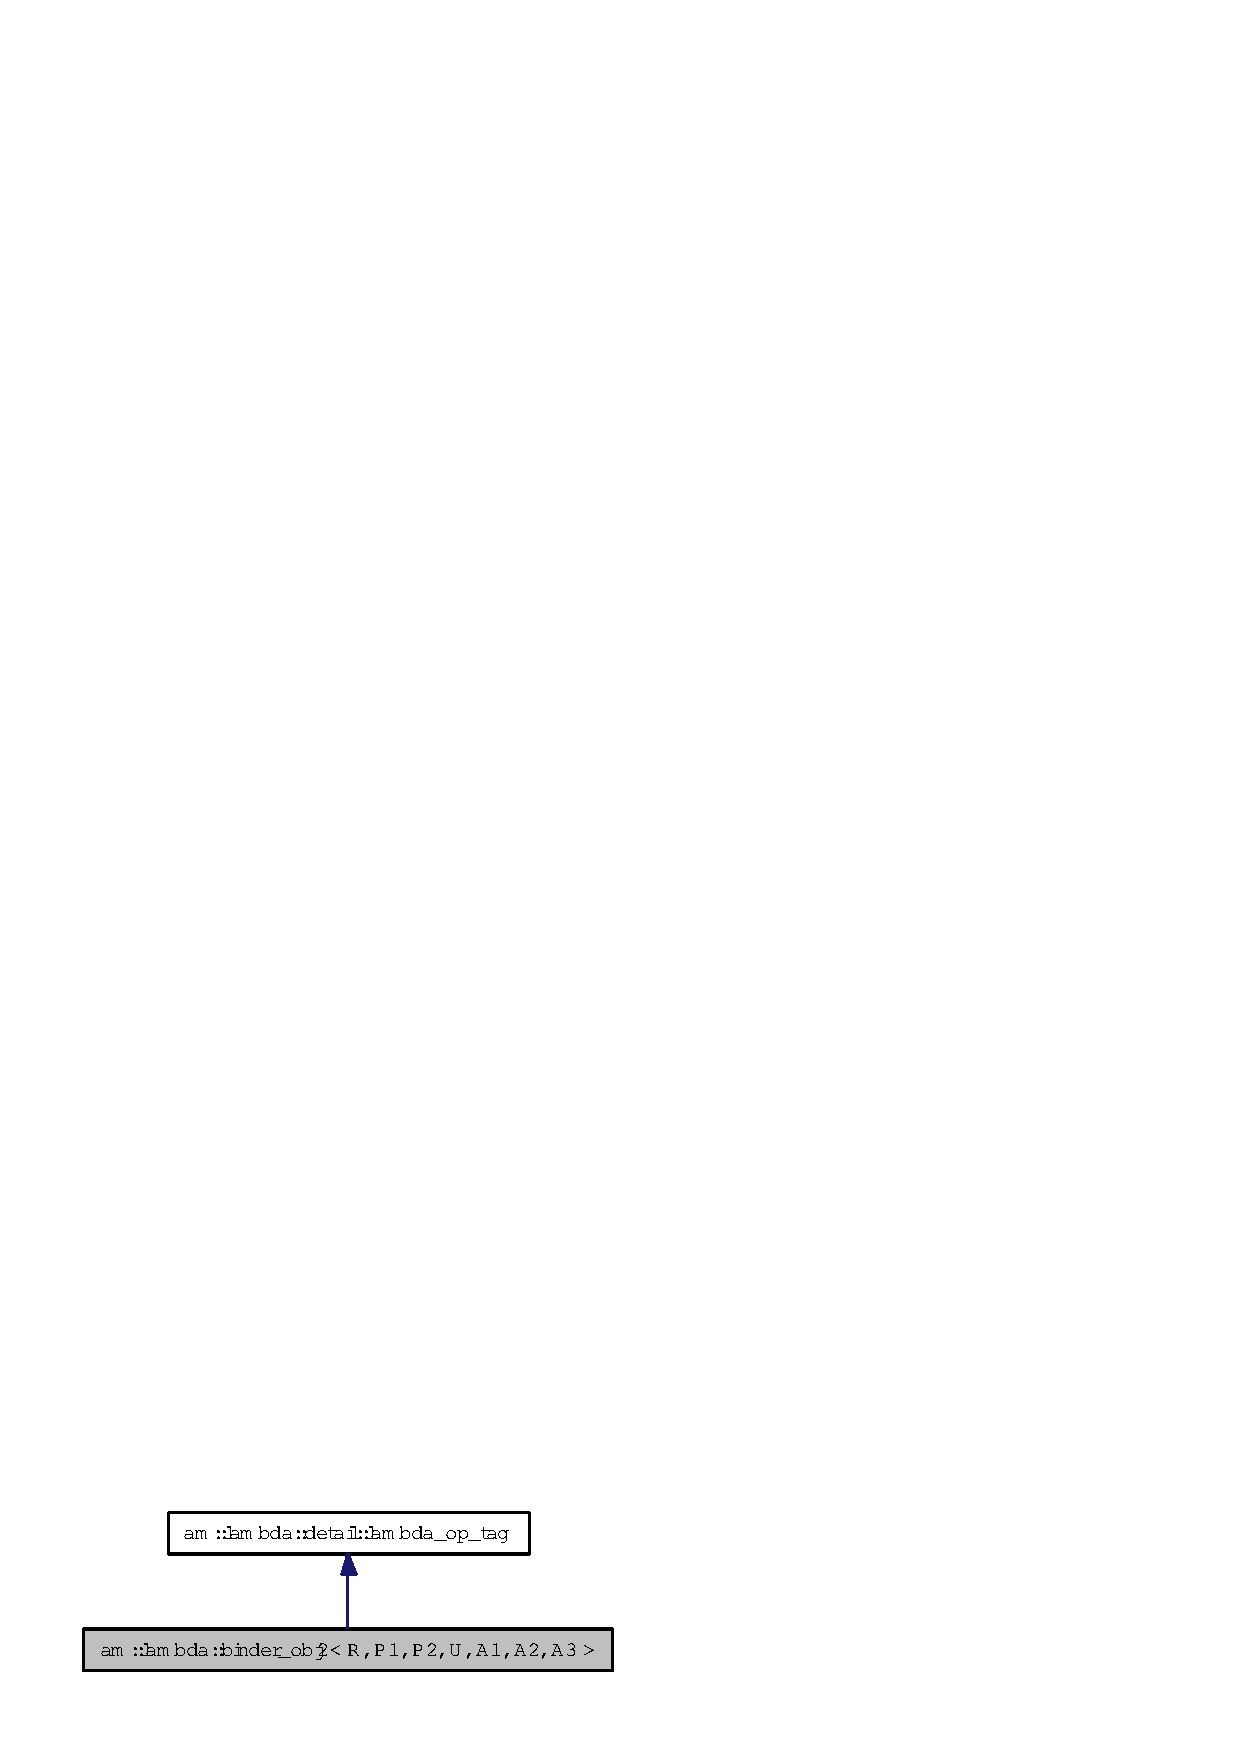
\includegraphics[width=149pt]{structam_1_1lambda_1_1binder__obj2__inherit__graph}
\end{center}
\end{figure}
Collaboration diagram for am::lambda::binder\_\-obj2$<$ R, P1, P2, U, A1, A2, A3 $>$:\begin{figure}[H]
\begin{center}
\leavevmode
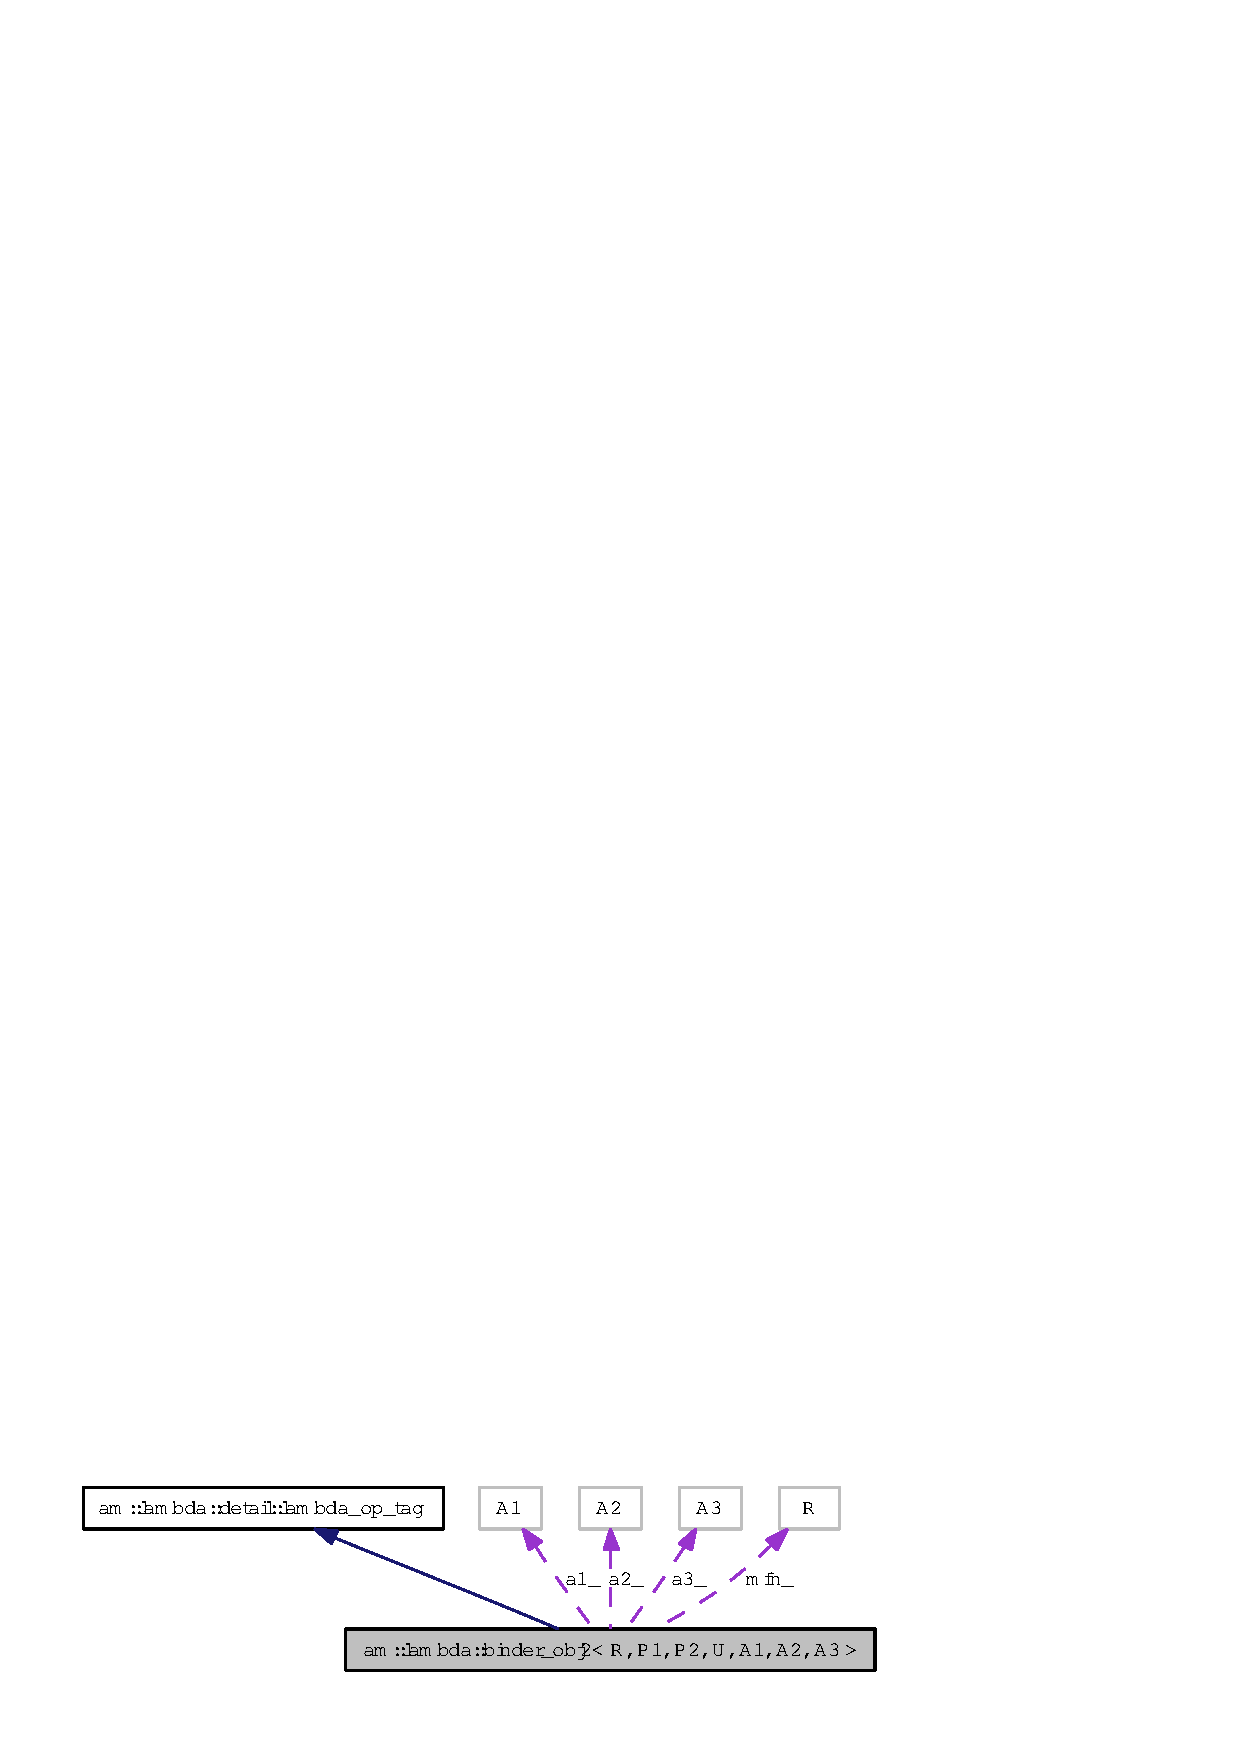
\includegraphics[width=212pt]{structam_1_1lambda_1_1binder__obj2__coll__graph}
\end{center}
\end{figure}
\subsection*{Public Types}
\begin{CompactItemize}
\item 
typedef detail::binder\_\-impl$<$ R $>$::result\_\-type \textbf{result\_\-type}\label{structam_1_1lambda_1_1binder__obj2_84617801bf8dc830ba9298500150b5b3}

\end{CompactItemize}
\subsection*{Public Member Functions}
\begin{CompactItemize}
\item 
\textbf{binder\_\-obj2} (R(U::$\ast$mfn)(P1, P2), A1 a1, A2 a2, A3 a3)\label{structam_1_1lambda_1_1binder__obj2_b6c3d3cf87cf2043109bb3ffc50600f8}

\item 
template$<$class T1, class T2, class T3$>$ result\_\-type \textbf{operator()} (T1 t1, T2 t2, T3 t3) const \label{structam_1_1lambda_1_1binder__obj2_85f7162e6770a724fd7df21942d0db12}

\item 
template$<$class T1, class T2$>$ result\_\-type \textbf{operator()} (T1 t1, T2 t2) const\label{structam_1_1lambda_1_1binder__obj2_728524865a5534c28313682ca84a37cb}

\item 
template$<$class T1$>$ result\_\-type \textbf{operator()} (T1 t1) const \label{structam_1_1lambda_1_1binder__obj2_e24884808c9326ecea0ebbf01ad38433}

\item 
result\_\-type \textbf{operator()} () const\label{structam_1_1lambda_1_1binder__obj2_46d82ba146ffb7b2078ff54f5cd73864}

\end{CompactItemize}
\subsection*{Public Attributes}
\begin{CompactItemize}
\item 
R(U::$\ast$ \textbf{mfn\_\-} )(P1, P2)\label{structam_1_1lambda_1_1binder__obj2_e7121c748bbacb92001963df40d011c6}

\item 
A1 \textbf{a1\_\-}\label{structam_1_1lambda_1_1binder__obj2_33d2936d64731df2deb1ed60a5f41460}

\item 
A2 \textbf{a2\_\-}\label{structam_1_1lambda_1_1binder__obj2_e8126415b8f3afaa65ea1c03dbe16c2b}

\item 
A3 \textbf{a3\_\-}\label{structam_1_1lambda_1_1binder__obj2_e23e6873967450ae98681211bff38a3d}

\end{CompactItemize}


\subsection{Detailed Description}
\subsubsection*{template$<$typename R, typename P1, typename P2, typename U, typename A1, typename A2, typename A3$>$ struct am::lambda::binder\_\-obj2$<$ R, P1, P2, U, A1, A2, A3 $>$}

Binder for the member function which takes the first argument as object on which the member function is being called and two more arguments. 



The documentation for this struct was generated from the following file:\begin{CompactItemize}
\item 
{\bf lambda.hpp}\end{CompactItemize}

\section{am::lambda::binder\_\-obj3$<$ R, P1, P2, P3, U, A1, A2, A3, A4 $>$ Struct Template Reference}
\label{structam_1_1lambda_1_1binder__obj3}\index{am::lambda::binder_obj3@{am::lambda::binder\_\-obj3}}
{\tt \#include $<$lambda.hpp$>$}

Inherits {\bf am::lambda::detail::lambda\_\-op\_\-tag}.

Inheritance diagram for am::lambda::binder\_\-obj3$<$ R, P1, P2, P3, U, A1, A2, A3, A4 $>$:\begin{figure}[H]
\begin{center}
\leavevmode
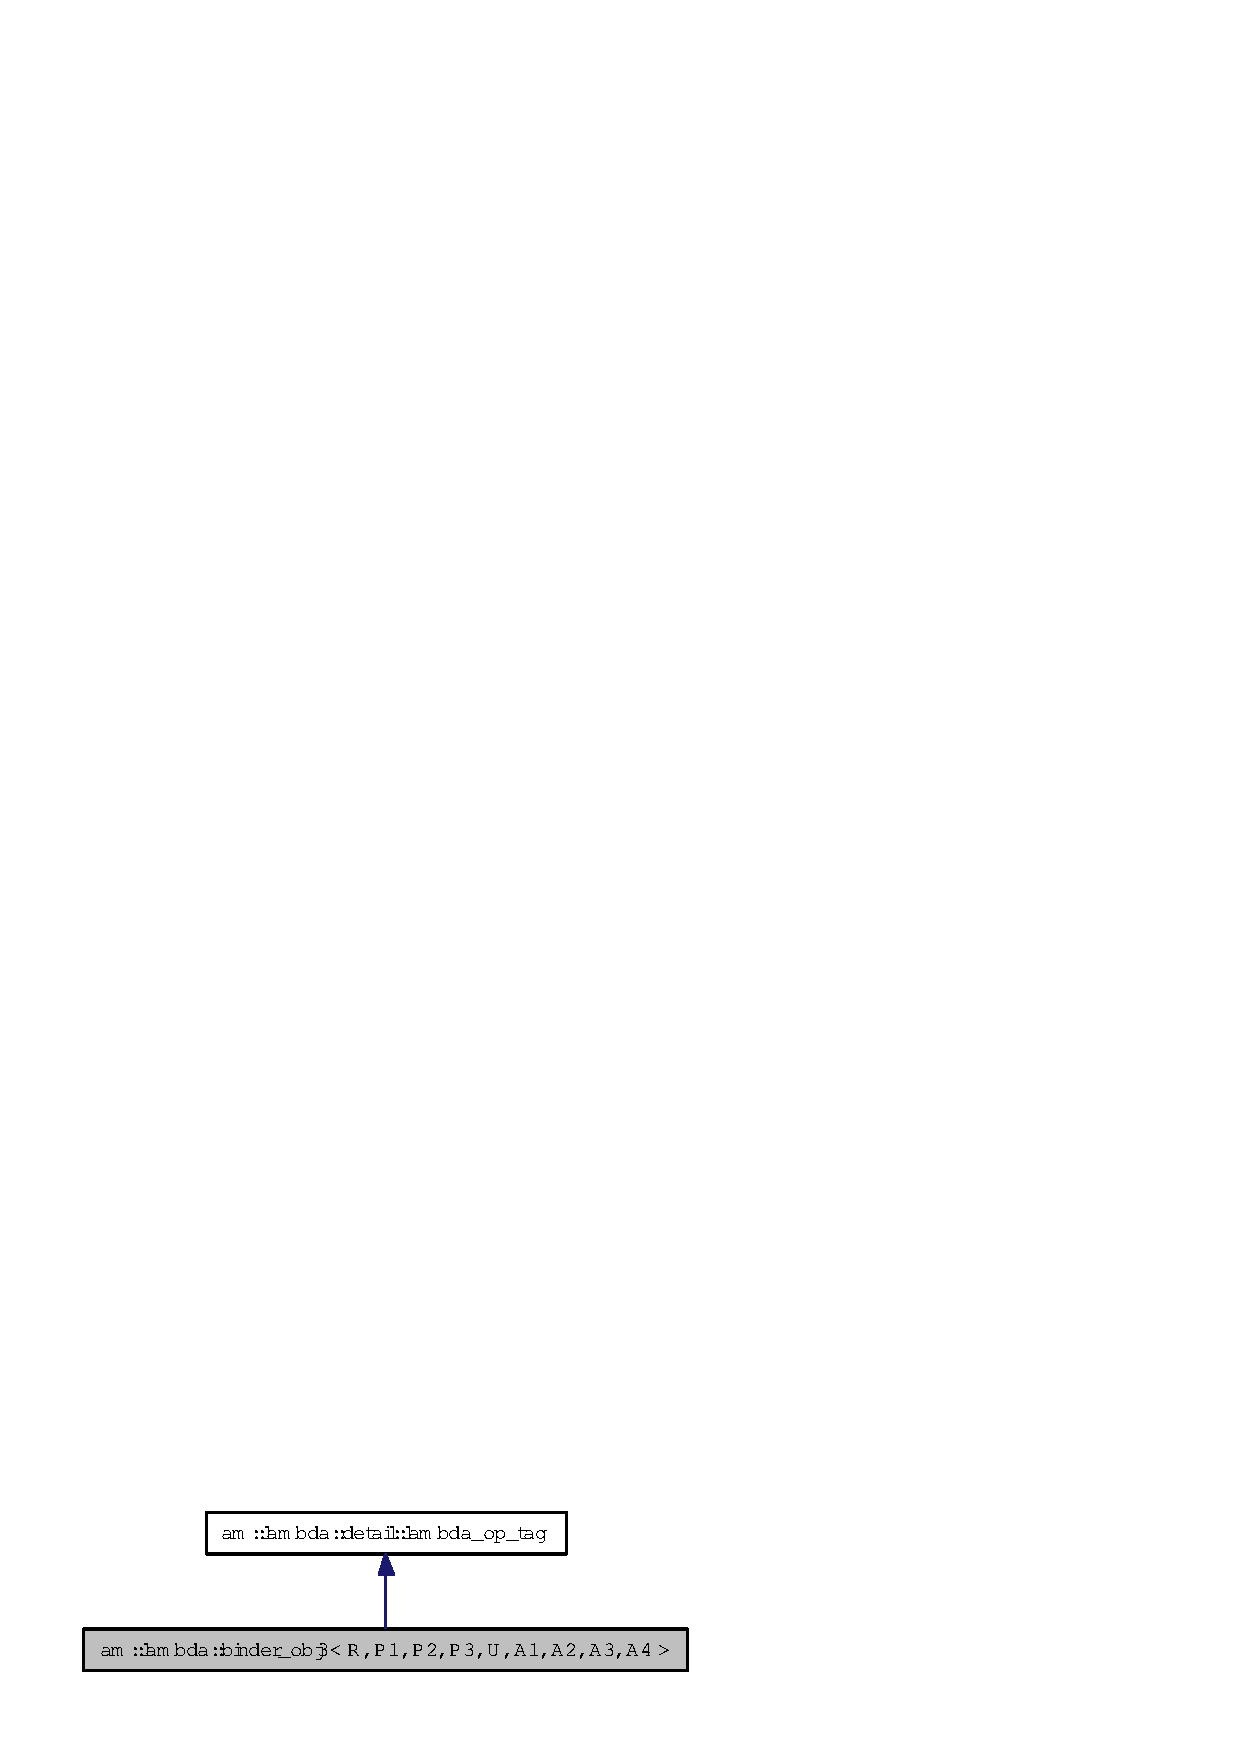
\includegraphics[width=167pt]{structam_1_1lambda_1_1binder__obj3__inherit__graph}
\end{center}
\end{figure}
Collaboration diagram for am::lambda::binder\_\-obj3$<$ R, P1, P2, P3, U, A1, A2, A3, A4 $>$:\begin{figure}[H]
\begin{center}
\leavevmode
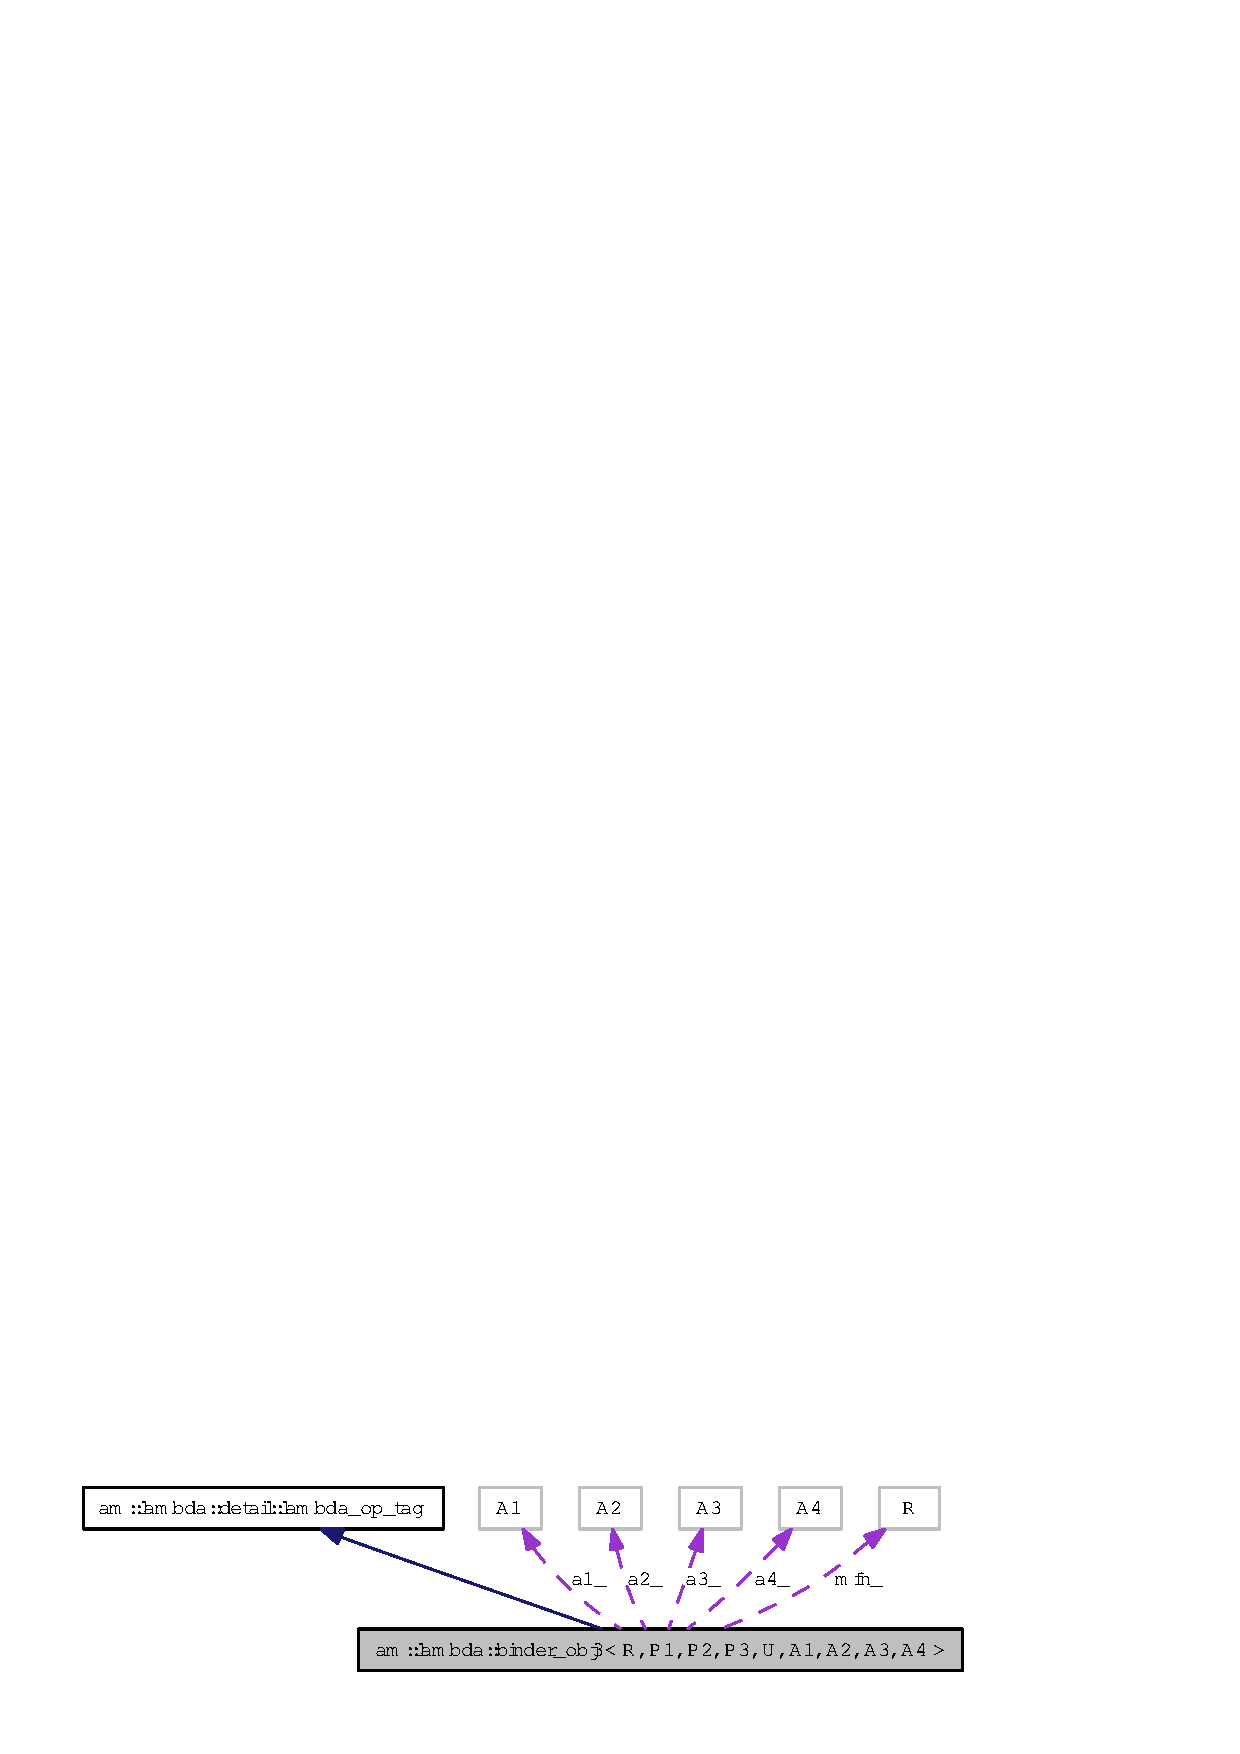
\includegraphics[width=233pt]{structam_1_1lambda_1_1binder__obj3__coll__graph}
\end{center}
\end{figure}
\subsection*{Public Types}
\begin{CompactItemize}
\item 
typedef detail::binder\_\-impl$<$ R $>$::result\_\-type \textbf{result\_\-type}\label{structam_1_1lambda_1_1binder__obj3_5c3870ec9614f57a734bd9f577cfdf30}

\end{CompactItemize}
\subsection*{Public Member Functions}
\begin{CompactItemize}
\item 
\textbf{binder\_\-obj3} (R(U::$\ast$mfn)(P1, P2, P3), A1 a1, A2 a2, A3 a3, A4 a4)\label{structam_1_1lambda_1_1binder__obj3_c5fcc482e43a36faf1939985c32a716d}

\item 
template$<$class T1, class T2, class T3$>$ result\_\-type \textbf{operator()} (T1 t1, T2 t2, T3 t3) const \label{structam_1_1lambda_1_1binder__obj3_64dacce5c3ea8d015b42cdbc903b0cb0}

\item 
template$<$class T1, class T2$>$ result\_\-type \textbf{operator()} (T1 t1, T2 t2) const\label{structam_1_1lambda_1_1binder__obj3_fd82b9f13adab9980950fa65218345a7}

\item 
template$<$class T1$>$ result\_\-type \textbf{operator()} (T1 t1) const \label{structam_1_1lambda_1_1binder__obj3_25fba29089b5f098cfc6497311c47f5f}

\item 
result\_\-type \textbf{operator()} () const\label{structam_1_1lambda_1_1binder__obj3_c6adcbfca05844b4e467a2f1facccdf8}

\end{CompactItemize}
\subsection*{Public Attributes}
\begin{CompactItemize}
\item 
R(U::$\ast$ \textbf{mfn\_\-} )(P1, P2, P3)\label{structam_1_1lambda_1_1binder__obj3_b7fb9cb1faa12f1791c64e3b65e6b83c}

\item 
A1 \textbf{a1\_\-}\label{structam_1_1lambda_1_1binder__obj3_cd739e72b4e47ce2c27a271b7cbe2541}

\item 
A2 \textbf{a2\_\-}\label{structam_1_1lambda_1_1binder__obj3_f504f1195118a5bd741922a683ba6bfb}

\item 
A3 \textbf{a3\_\-}\label{structam_1_1lambda_1_1binder__obj3_b625d13105628d14fa426aef1a52ae5b}

\item 
A4 \textbf{a4\_\-}\label{structam_1_1lambda_1_1binder__obj3_29397f2409045b66d1a46e77d3cab171}

\end{CompactItemize}


\subsection{Detailed Description}
\subsubsection*{template$<$typename R, typename P1, typename P2, typename P3, typename U, typename A1, typename A2, typename A3, typename A4$>$ struct am::lambda::binder\_\-obj3$<$ R, P1, P2, P3, U, A1, A2, A3, A4 $>$}

Binder for the member function which takes the first argument as object on which the member function is being called and three more arguments. 



The documentation for this struct was generated from the following file:\begin{CompactItemize}
\item 
{\bf lambda.hpp}\end{CompactItemize}

\section{am::condition Struct Reference}
\label{structam_1_1condition}\index{am::condition@{am::condition}}
Predicate.  


{\tt \#include $<$mate.hpp$>$}

\subsection*{Public Member Functions}
\begin{CompactItemize}
\item 
\textbf{condition} (bool expr)\label{structam_1_1condition_82253727f9840bf92be5fe9ac6f030f3}

\item 
template$<$class T$>$ bool \textbf{operator()} (T t) const \label{structam_1_1condition_b2ec8dd69ee9d01f6e063e8ff134aa8e}

\item 
bool \textbf{operator()} () const\label{structam_1_1condition_77b22c0ae8b8f417243fa1418041da9a}

\end{CompactItemize}
\subsection*{Public Attributes}
\begin{CompactItemize}
\item 
bool \textbf{expr\_\-}\label{structam_1_1condition_4847e0ef9b08433407f602ebf9825c18}

\end{CompactItemize}


\subsection{Detailed Description}
Predicate. 

Convert a boolean expression into null-nary or unary predicate. 



The documentation for this struct was generated from the following file:\begin{CompactItemize}
\item 
{\bf mate.hpp}\end{CompactItemize}

\section{am::lambda::condition Struct Reference}
\label{structam_1_1lambda_1_1condition}\index{am::lambda::condition@{am::lambda::condition}}
Predicate.  


{\tt \#include $<$lambda.hpp$>$}

Inherits {\bf am::lambda::detail::lambda\_\-op\_\-tag}.

Inheritance diagram for am::lambda::condition:\begin{figure}[H]
\begin{center}
\leavevmode
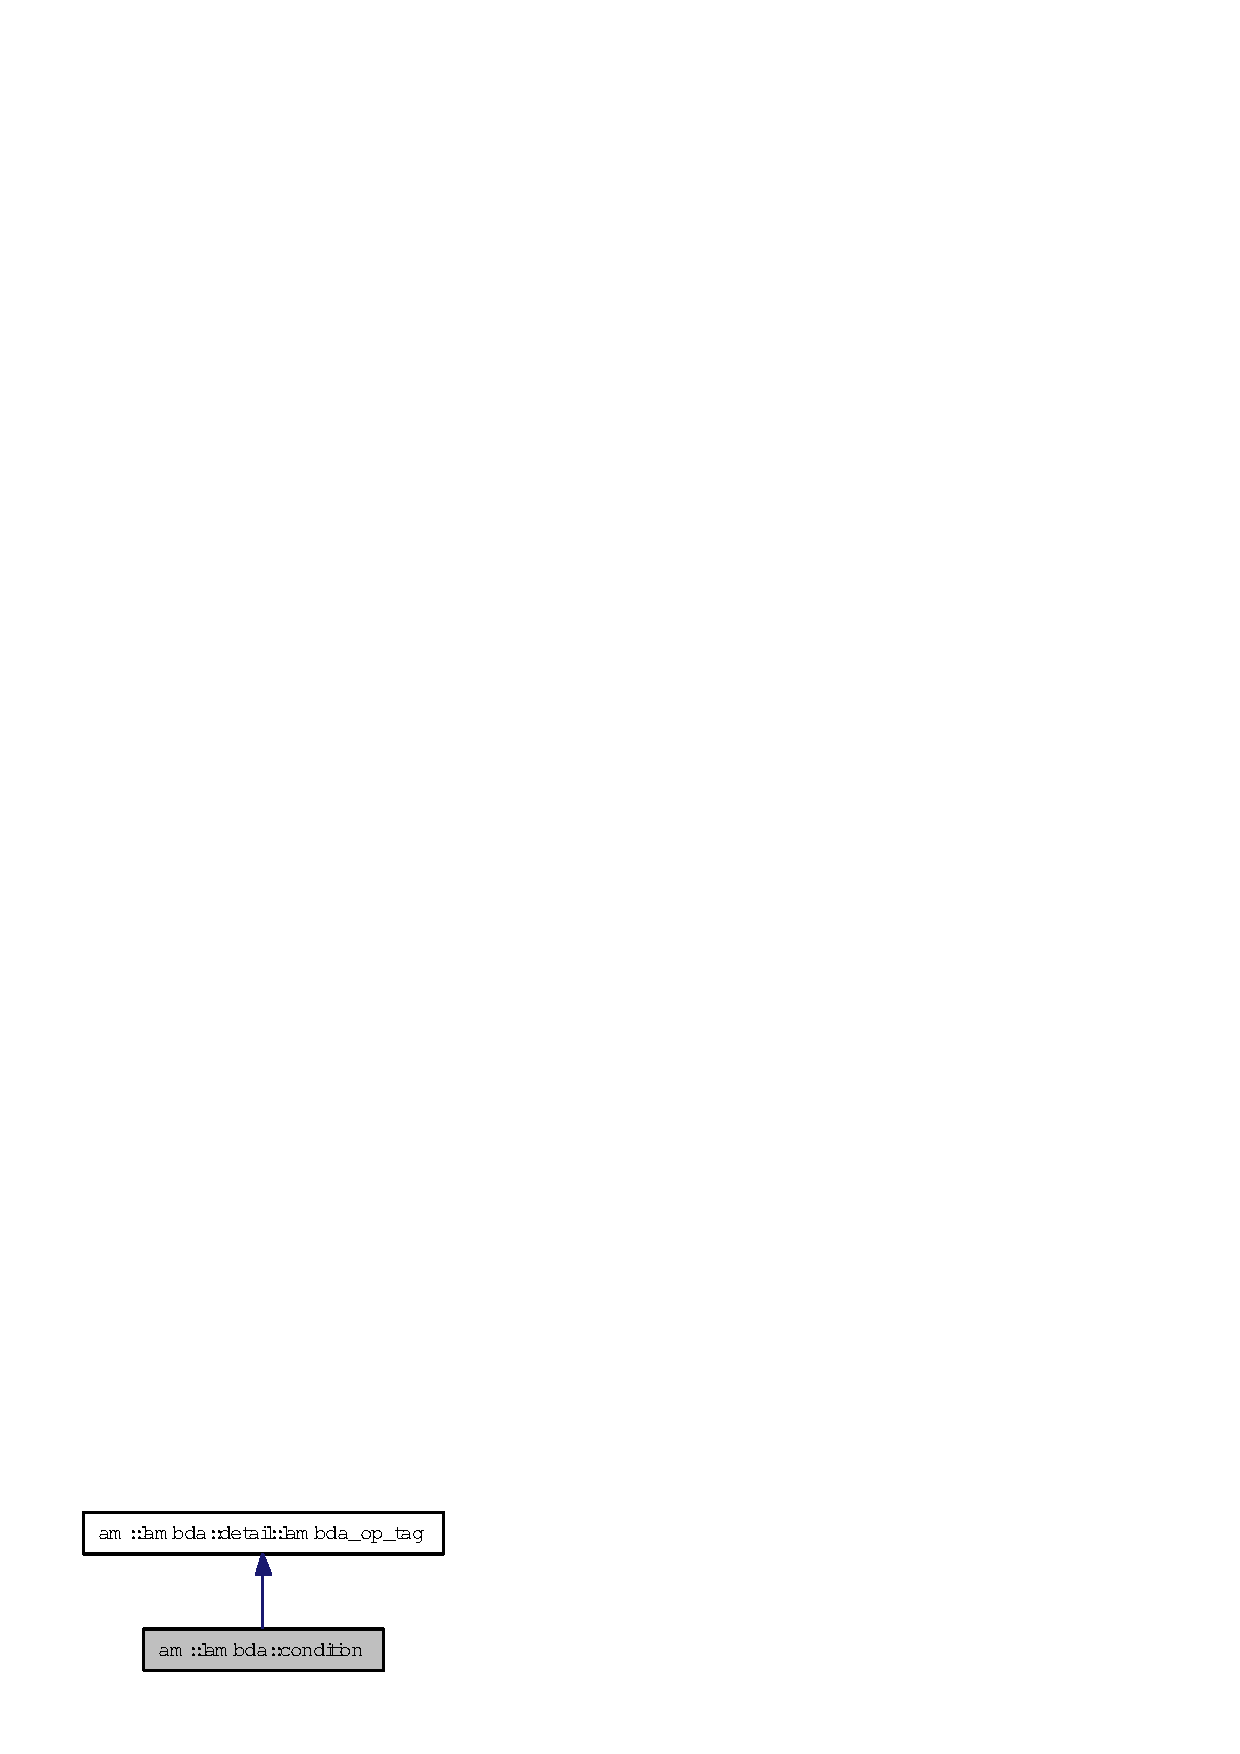
\includegraphics[width=108pt]{structam_1_1lambda_1_1condition__inherit__graph}
\end{center}
\end{figure}
Collaboration diagram for am::lambda::condition:\begin{figure}[H]
\begin{center}
\leavevmode
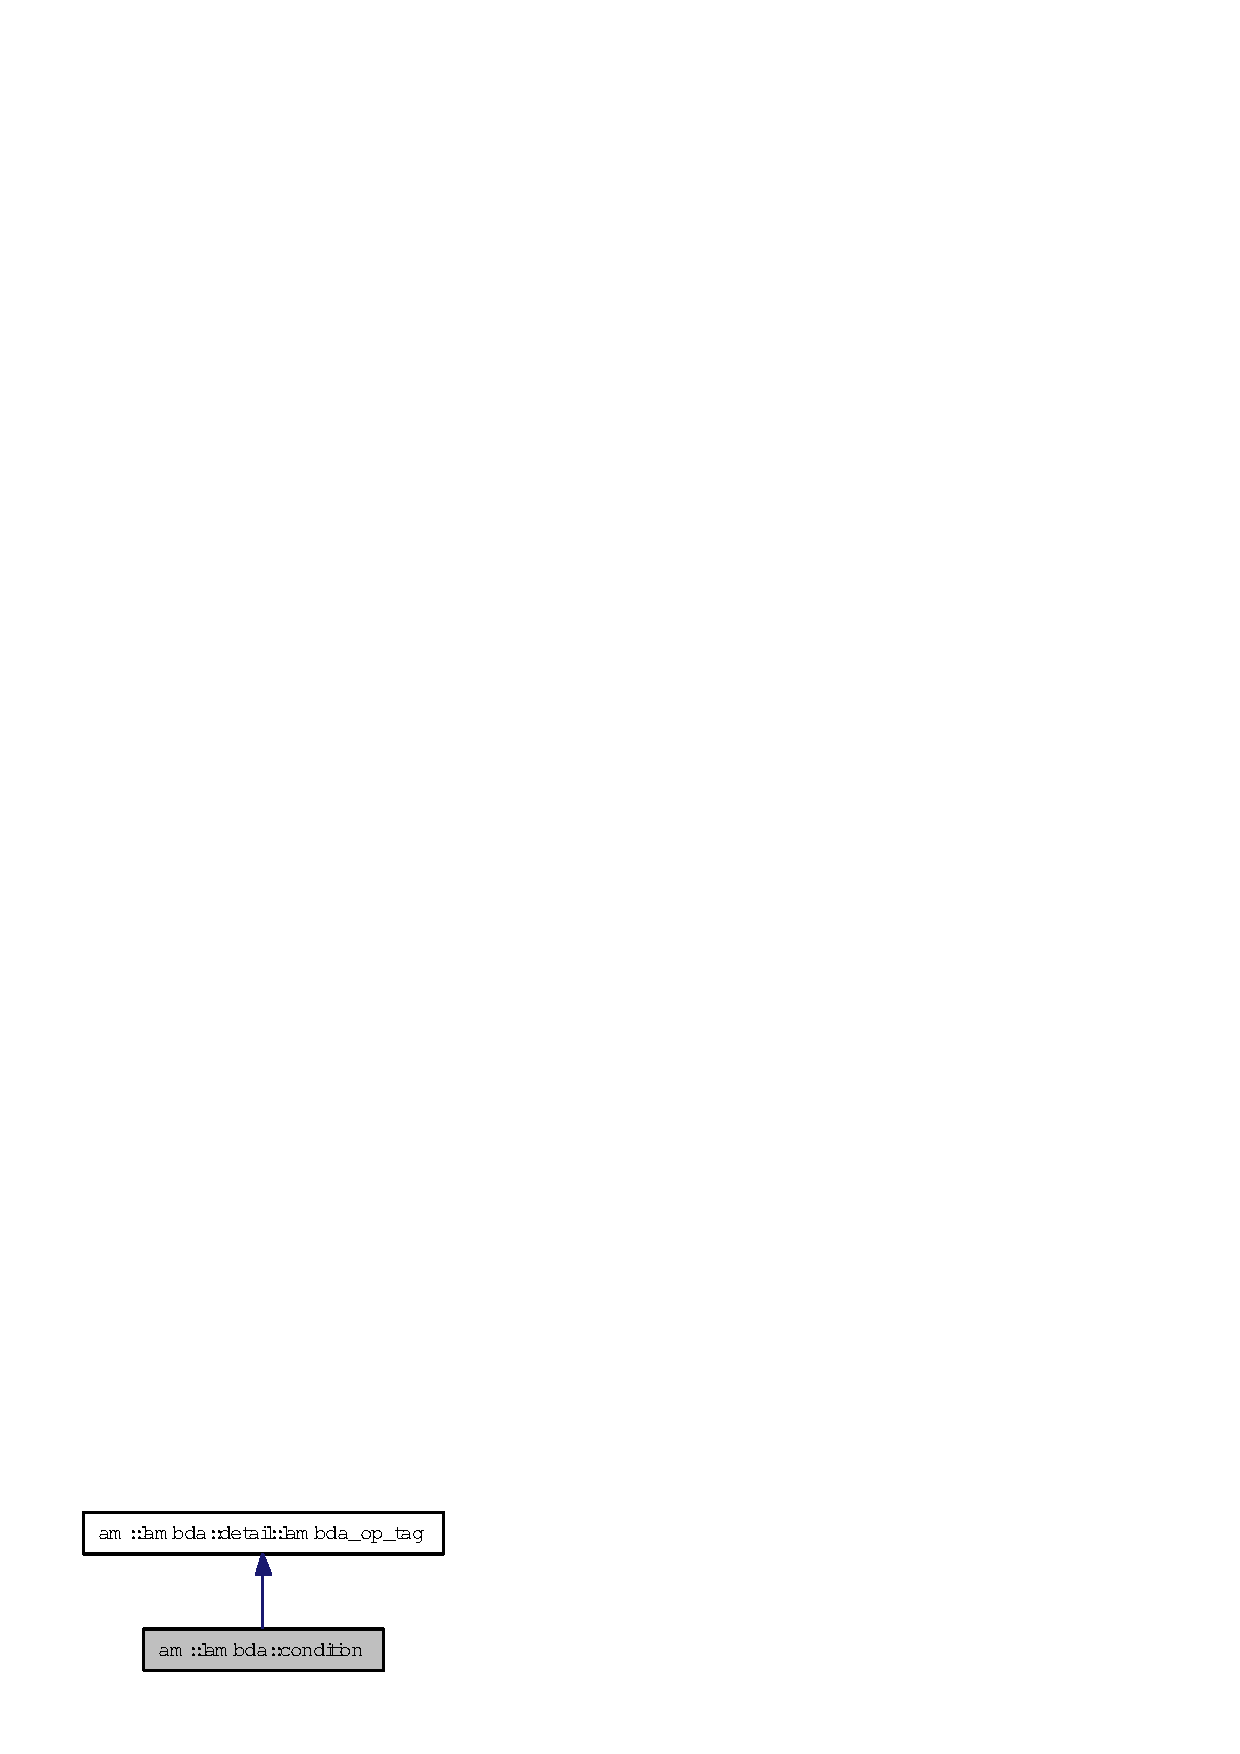
\includegraphics[width=108pt]{structam_1_1lambda_1_1condition__coll__graph}
\end{center}
\end{figure}
\subsection*{Public Member Functions}
\begin{CompactItemize}
\item 
\textbf{condition} (bool b)\label{structam_1_1lambda_1_1condition_e40f01ee1d36564ae8fc2741d810ee67}

\item 
template$<$class T1, class T2, class T3$>$ bool \textbf{operator()} (T1, T2, T3) const\label{structam_1_1lambda_1_1condition_01b6a3632c9427e5751d25553c0b7299}

\item 
template$<$class T1, class T2$>$ bool \textbf{operator()} (T1, T2) const\label{structam_1_1lambda_1_1condition_7c9b36804edcb13cd6d92de83557abd9}

\item 
template$<$class T1$>$ bool \textbf{operator()} (T1) const\label{structam_1_1lambda_1_1condition_08a614f29cafff6959b43fc64485e40b}

\item 
bool \textbf{operator()} () const\label{structam_1_1lambda_1_1condition_19e3c55b10f5c5edf3fdf099d26a365c}

\end{CompactItemize}
\subsection*{Public Attributes}
\begin{CompactItemize}
\item 
bool \textbf{b\_\-}\label{structam_1_1lambda_1_1condition_19014c303208f7d24845652348737106}

\end{CompactItemize}


\subsection{Detailed Description}
Predicate. 

Convert a boolean expression into null-nary or unary predicate. 



The documentation for this struct was generated from the following file:\begin{CompactItemize}
\item 
{\bf lambda.hpp}\end{CompactItemize}

\section{am::lambda::detail::if\_\- Struct Reference}
\label{structam_1_1lambda_1_1detail_1_1if__}\index{am::lambda::detail::if_@{am::lambda::detail::if\_\-}}
{\tt \#include $<$lambda.hpp$>$}



\subsection{Detailed Description}
\begin{Desc}
\item[For internal use only.]
if meta template class. Select type according to the boolean condition. \end{Desc}




The documentation for this struct was generated from the following file:\begin{CompactItemize}
\item 
{\bf lambda.hpp}\end{CompactItemize}

\section{am::lambda::detail::is\_\-lambda\_\-op$<$ T $>$ Struct Template Reference}
\label{structam_1_1lambda_1_1detail_1_1is__lambda__op}\index{am::lambda::detail::is_lambda_op@{am::lambda::detail::is\_\-lambda\_\-op}}
{\tt \#include $<$lambda.hpp$>$}

Collaboration diagram for am::lambda::detail::is\_\-lambda\_\-op$<$ T $>$:\begin{figure}[H]
\begin{center}
\leavevmode
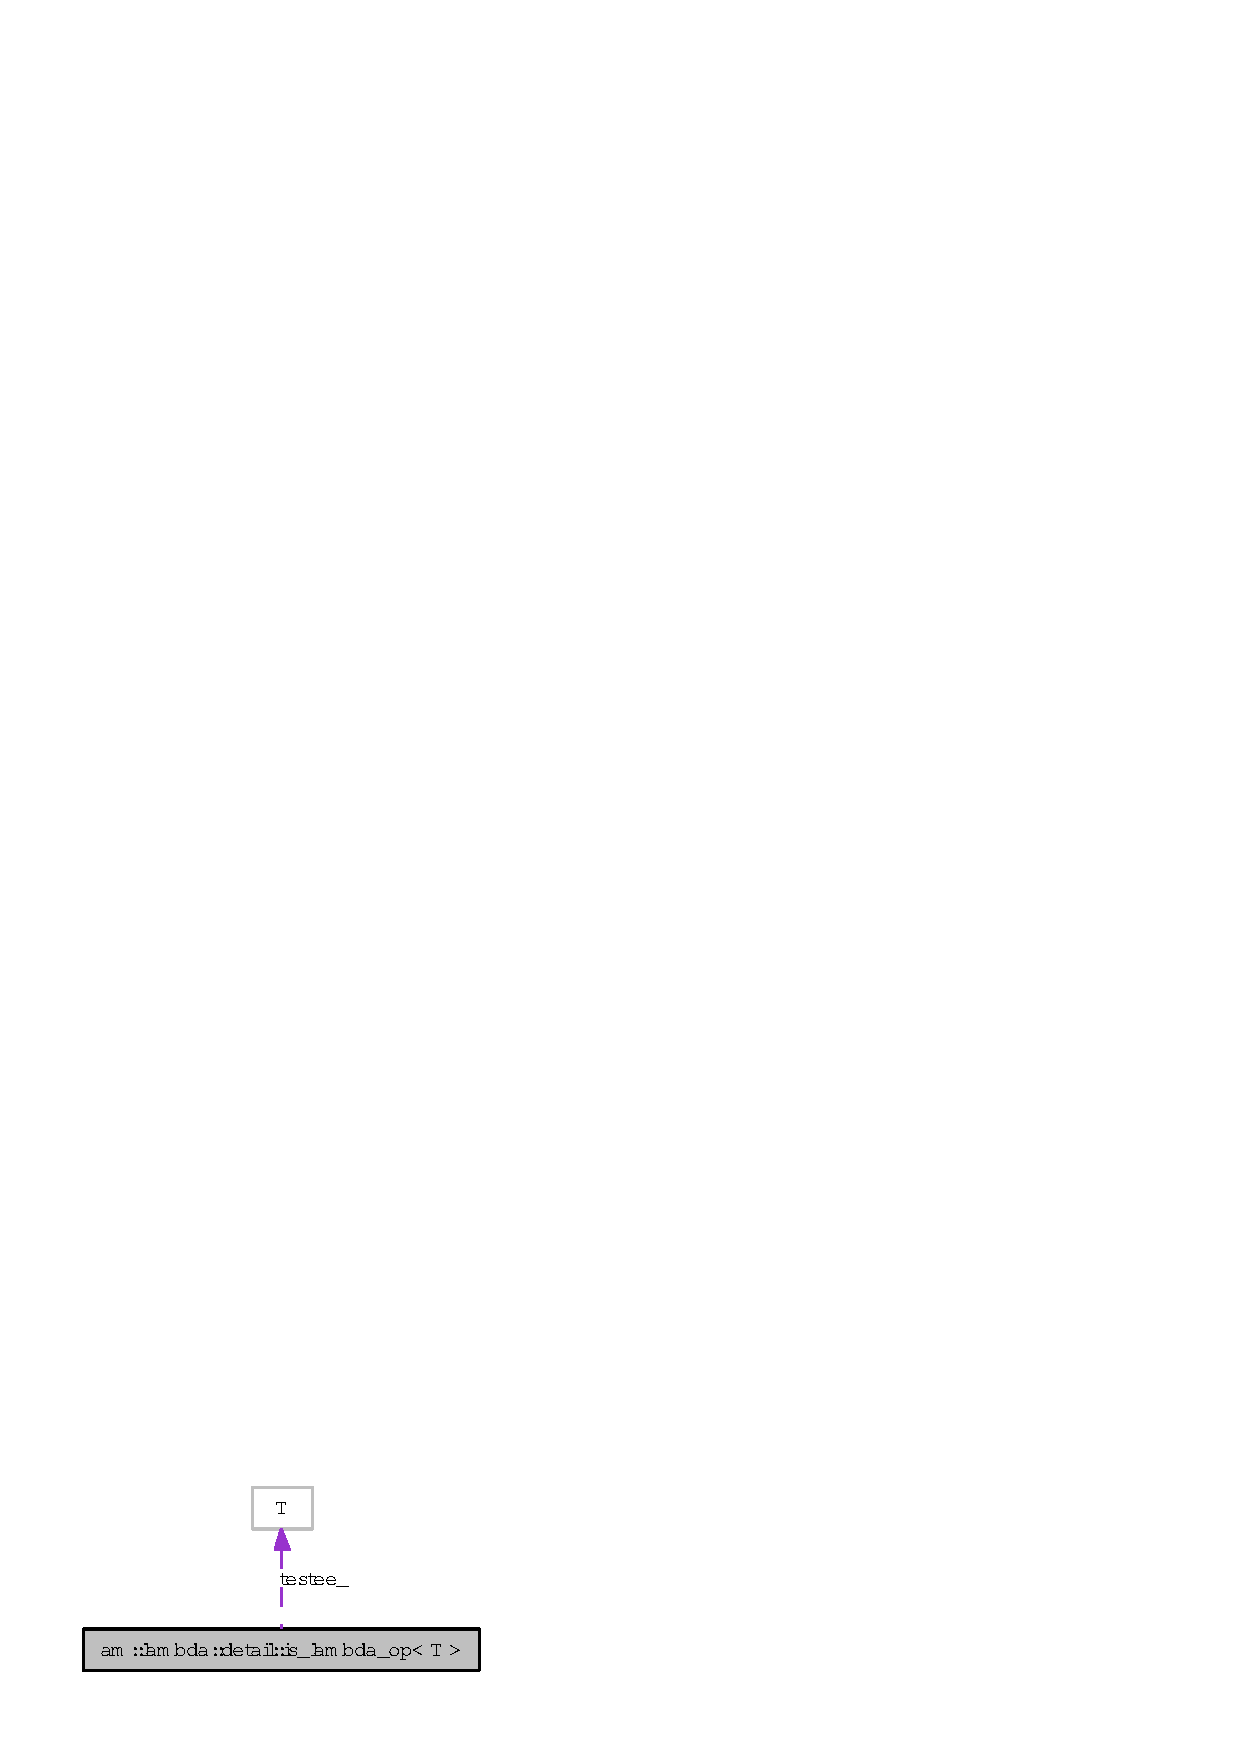
\includegraphics[width=117pt]{structam_1_1lambda_1_1detail_1_1is__lambda__op__coll__graph}
\end{center}
\end{figure}
\subsection*{Public Types}
\begin{CompactItemize}
\item 
enum \{ \textbf{value} =  ( sizeof( char ) == sizeof( tester\_\-( testee\_\- ) ) )
 \}
\end{CompactItemize}
\subsection*{Static Public Member Functions}
\begin{CompactItemize}
\item 
static char \textbf{tester\_\-} ({\bf lambda\_\-op\_\-tag} \&)\label{structam_1_1lambda_1_1detail_1_1is__lambda__op_3129188c36702ff8c61db717a7a6aa2d}

\item 
static int \textbf{tester\_\-} (...)\label{structam_1_1lambda_1_1detail_1_1is__lambda__op_e346e2ba0cc00fe21bfb53ecbe373a2b}

\end{CompactItemize}
\subsection*{Static Public Attributes}
\begin{CompactItemize}
\item 
static T \textbf{testee\_\-}\label{structam_1_1lambda_1_1detail_1_1is__lambda__op_d55b3d039563337d911da9122255ce84}

\end{CompactItemize}


\subsection{Detailed Description}
\subsubsection*{template$<$class T$>$ struct am::lambda::detail::is\_\-lambda\_\-op$<$ T $>$}

\begin{Desc}
\item[For internal use only.]
Determines whether or not the specified template type is a derived from \doxyref{lambda\_\-op\_\-tag}{p.}{structam_1_1lambda_1_1detail_1_1lambda__op__tag}. \end{Desc}




The documentation for this struct was generated from the following file:\begin{CompactItemize}
\item 
{\bf lambda.hpp}\end{CompactItemize}

\section{am::lambda::detail::lambda\_\-op\_\-tag Struct Reference}
\label{structam_1_1lambda_1_1detail_1_1lambda__op__tag}\index{am::lambda::detail::lambda_op_tag@{am::lambda::detail::lambda\_\-op\_\-tag}}
{\tt \#include $<$lambda.hpp$>$}

Inherited by {\bf am::lambda::binder0$<$ R $>$}, {\bf am::lambda::binder1$<$ R, P1, A1 $>$}, {\bf am::lambda::binder2$<$ R, P1, P2, A1, A2 $>$}, {\bf am::lambda::binder3$<$ R, P1, P2, P3, A1, A2, A3 $>$}, {\bf am::lambda::binder\_\-const\_\-obj0$<$ R, U, A1 $>$}, {\bf am::lambda::binder\_\-const\_\-obj1$<$ R, P1, U, A1, A2 $>$}, {\bf am::lambda::binder\_\-const\_\-obj2$<$ R, P1, P2, U, A1, A2, A3 $>$}, {\bf am::lambda::binder\_\-const\_\-obj3$<$ R, P1, P2, P3, U, A1, A2, A3, A4 $>$}, {\bf am::lambda::binder\_\-obj0$<$ R, U, A1 $>$}, {\bf am::lambda::binder\_\-obj1$<$ R, P1, U, A1, A2 $>$}, {\bf am::lambda::binder\_\-obj2$<$ R, P1, P2, U, A1, A2, A3 $>$}, {\bf am::lambda::binder\_\-obj3$<$ R, P1, P2, P3, U, A1, A2, A3, A4 $>$}, {\bf am::lambda::condition}, {\bf am::lambda::pf\_\-memdata$<$ P, O, U $>$}, {\bf am::lambda::pf\_\-memdata$<$ P, O, U $>$::address\_\-of}, {\bf am::lambda::var\_\-type1::address\_\-of}, {\bf am::lambda::var\_\-type2::address\_\-of}, and {\bf am::lambda::var\_\-type3::address\_\-of}.

Inheritance diagram for am::lambda::detail::lambda\_\-op\_\-tag:\begin{figure}[H]
\begin{center}
\leavevmode
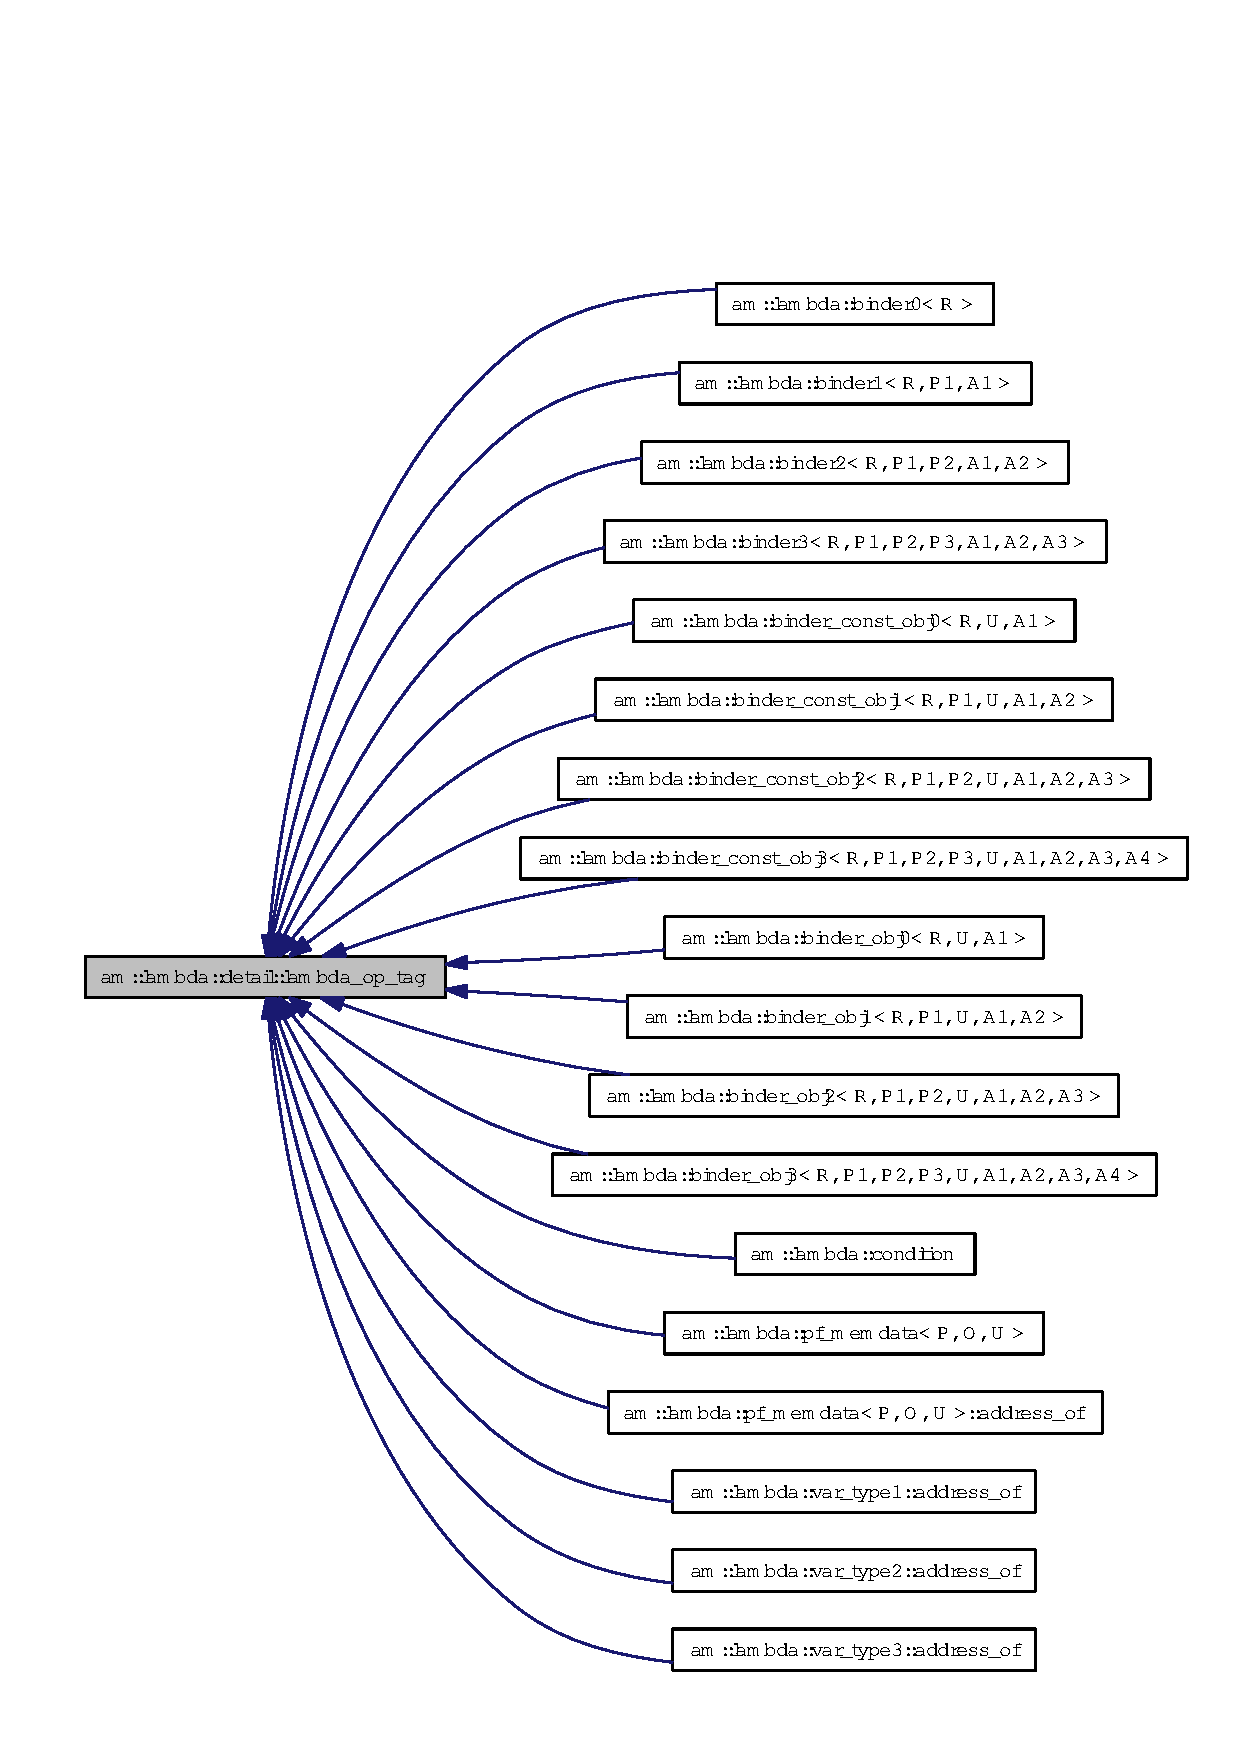
\includegraphics[width=287pt]{structam_1_1lambda_1_1detail_1_1lambda__op__tag__inherit__graph}
\end{center}
\end{figure}


\subsection{Detailed Description}
\begin{Desc}
\item[For internal use only.]
Tag of lambda operator. All lambda pure functions are derived from \doxyref{lambda\_\-op\_\-tag}{p.}{structam_1_1lambda_1_1detail_1_1lambda__op__tag}. \end{Desc}




The documentation for this struct was generated from the following file:\begin{CompactItemize}
\item 
{\bf lambda.hpp}\end{CompactItemize}

\section{am::lambda::detail::lambda\_\-val$<$ V $>$ Struct Template Reference}
\label{structam_1_1lambda_1_1detail_1_1lambda__val}\index{am::lambda::detail::lambda_val@{am::lambda::detail::lambda\_\-val}}
{\tt \#include $<$lambda.hpp$>$}

Collaboration diagram for am::lambda::detail::lambda\_\-val$<$ V $>$:\begin{figure}[H]
\begin{center}
\leavevmode
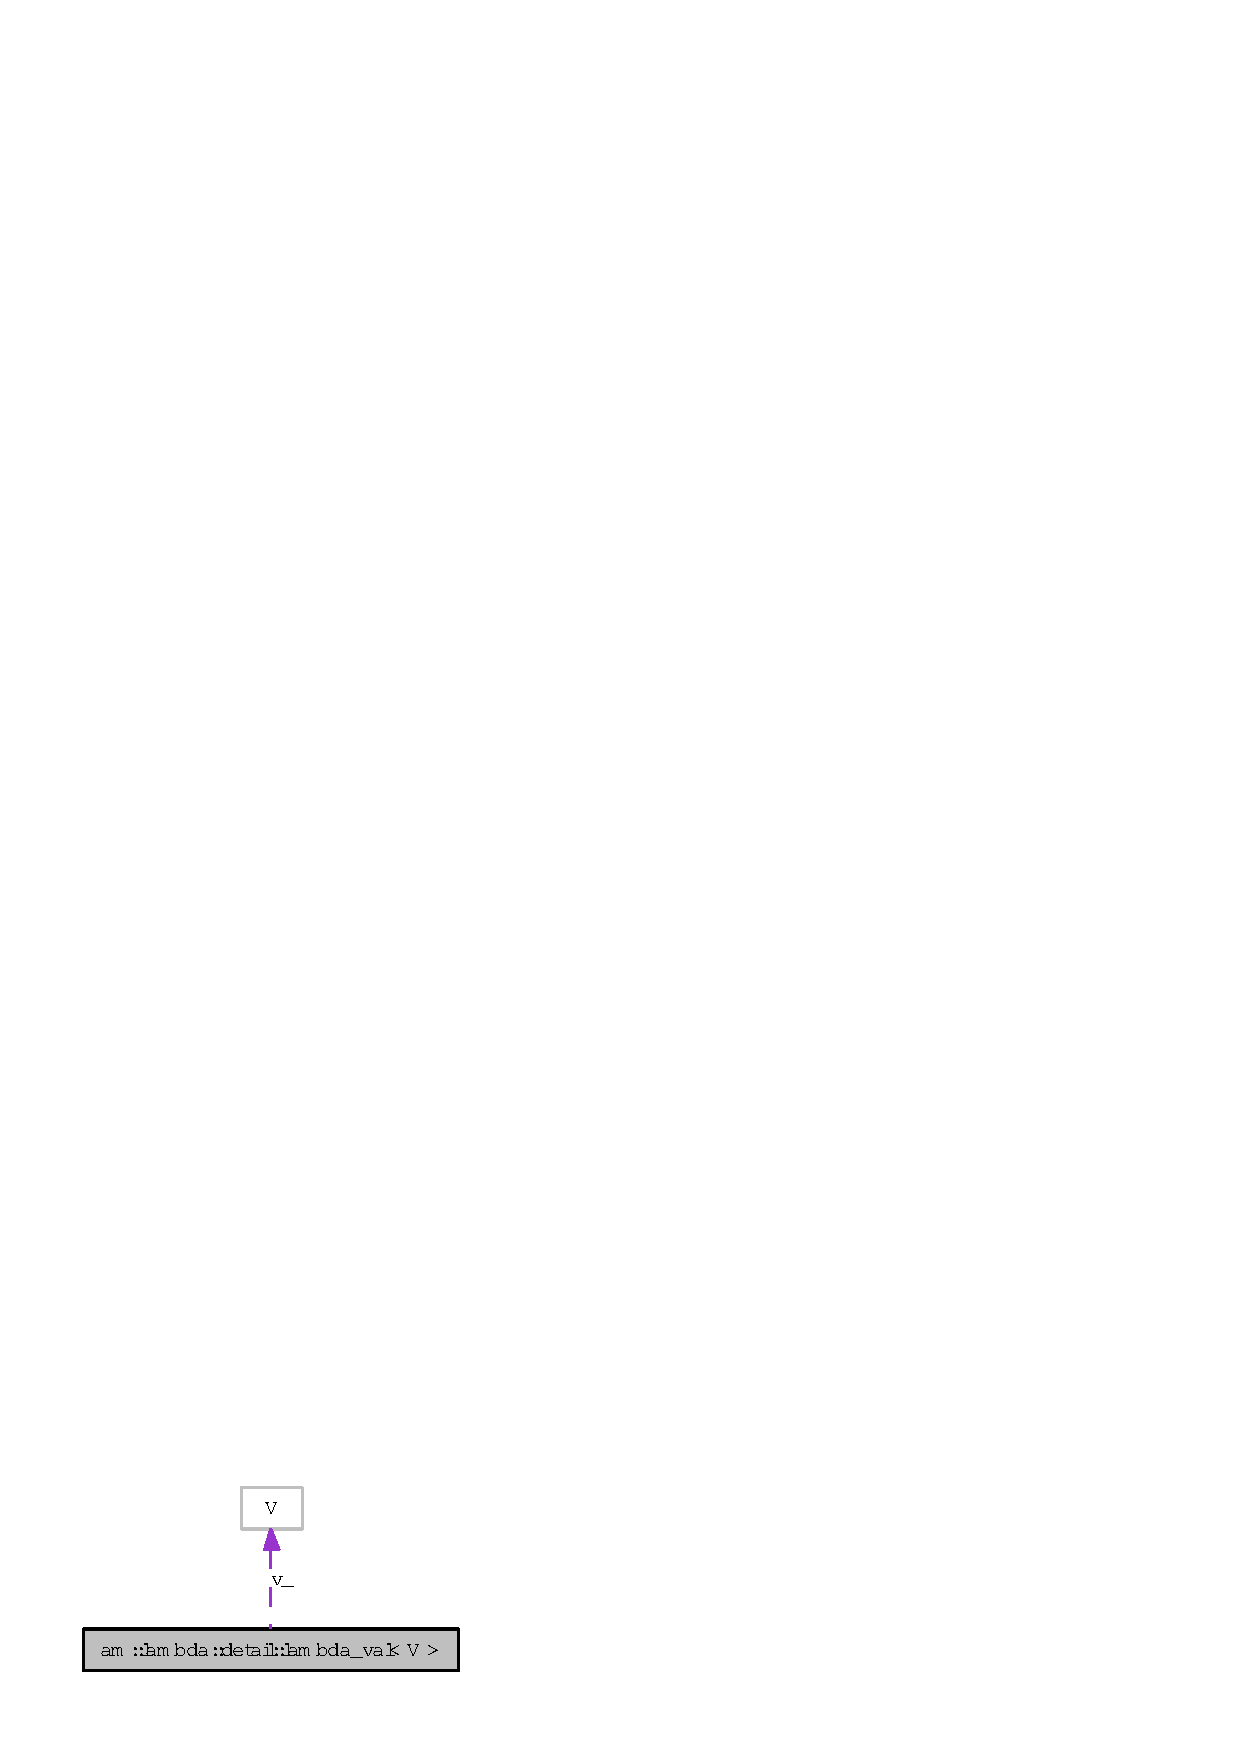
\includegraphics[width=112pt]{structam_1_1lambda_1_1detail_1_1lambda__val__coll__graph}
\end{center}
\end{figure}
\subsection*{Public Member Functions}
\begin{CompactItemize}
\item 
\textbf{lambda\_\-val} (V v)\label{structam_1_1lambda_1_1detail_1_1lambda__val_7152b6d4b085a10c679da302ebdeefac}

\item 
template$<$class T1, class T2, class T3$>$ V \textbf{operator()} (T1, T2, T3) const\label{structam_1_1lambda_1_1detail_1_1lambda__val_b831b0cc665d247776a5d0af6649ea7e}

\item 
template$<$class T1, class T2$>$ V \textbf{operator()} (T1, T2) const\label{structam_1_1lambda_1_1detail_1_1lambda__val_7dbcaa00f48521394febabb47a7779c9}

\item 
template$<$class T1$>$ V \textbf{operator()} (T1) const\label{structam_1_1lambda_1_1detail_1_1lambda__val_e1f756565171002df3161eeb0ae772da}

\item 
V \textbf{operator()} () const\label{structam_1_1lambda_1_1detail_1_1lambda__val_88d28ac1d9f6617f0a85b981db82cdfe}

\end{CompactItemize}
\subsection*{Public Attributes}
\begin{CompactItemize}
\item 
V \textbf{v\_\-}\label{structam_1_1lambda_1_1detail_1_1lambda__val_683416856f8594b8f4a17e50ba53833c}

\end{CompactItemize}


\subsection{Detailed Description}
\subsubsection*{template$<$class V$>$ struct am::lambda::detail::lambda\_\-val$<$ V $>$}

\begin{Desc}
\item[For internal use only.]
Lambda value. \end{Desc}




The documentation for this struct was generated from the following file:\begin{CompactItemize}
\item 
{\bf lambda.hpp}\end{CompactItemize}

\section{am::mate$<$ R $>$ Class Template Reference}
\label{classam_1_1mate}\index{am::mate@{am::mate}}
Mates a host function with the mate function object.  


{\tt \#include $<$mate.hpp$>$}

Inherits {\bf am::detail::mate\_\-base}.

Inheritance diagram for am::mate$<$ R $>$:\begin{figure}[H]
\begin{center}
\leavevmode
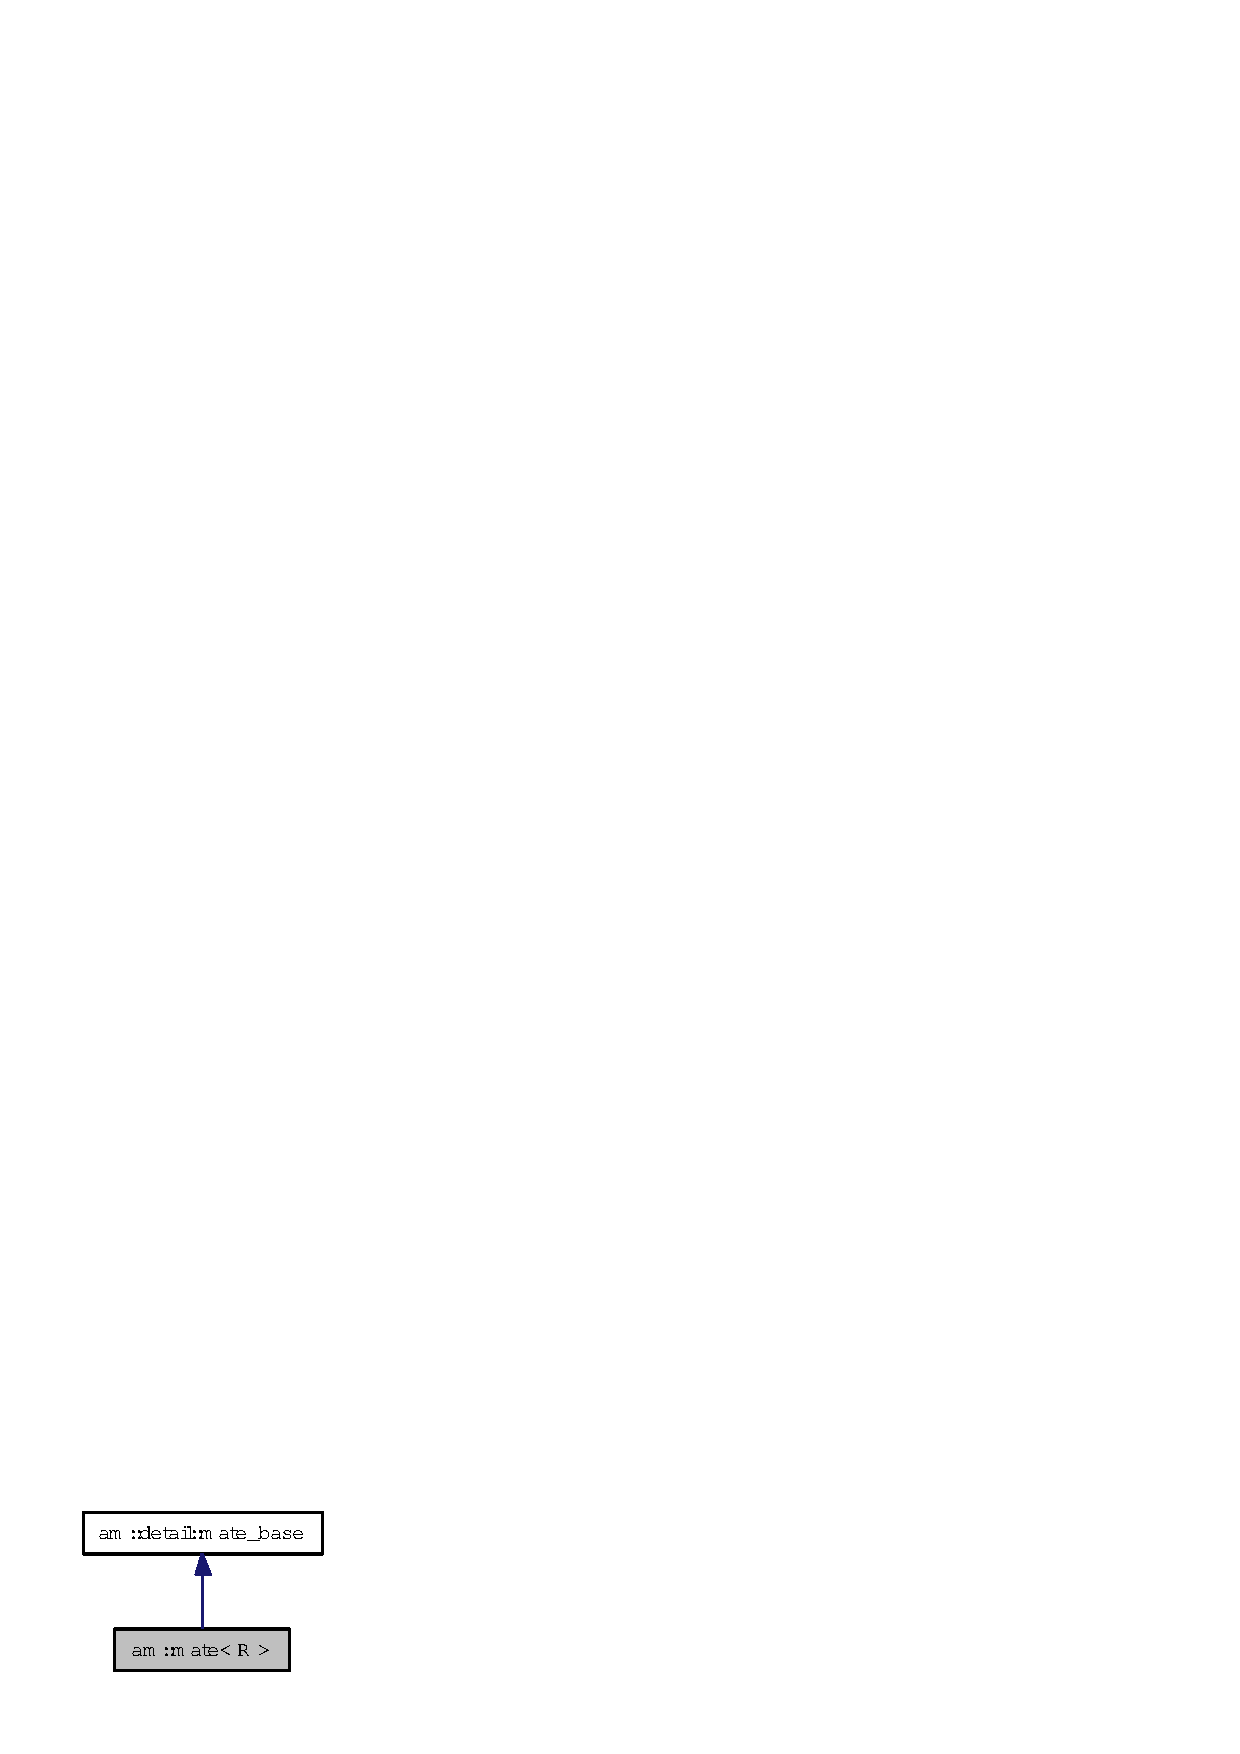
\includegraphics[width=79pt]{classam_1_1mate__inherit__graph}
\end{center}
\end{figure}
Collaboration diagram for am::mate$<$ R $>$:\begin{figure}[H]
\begin{center}
\leavevmode
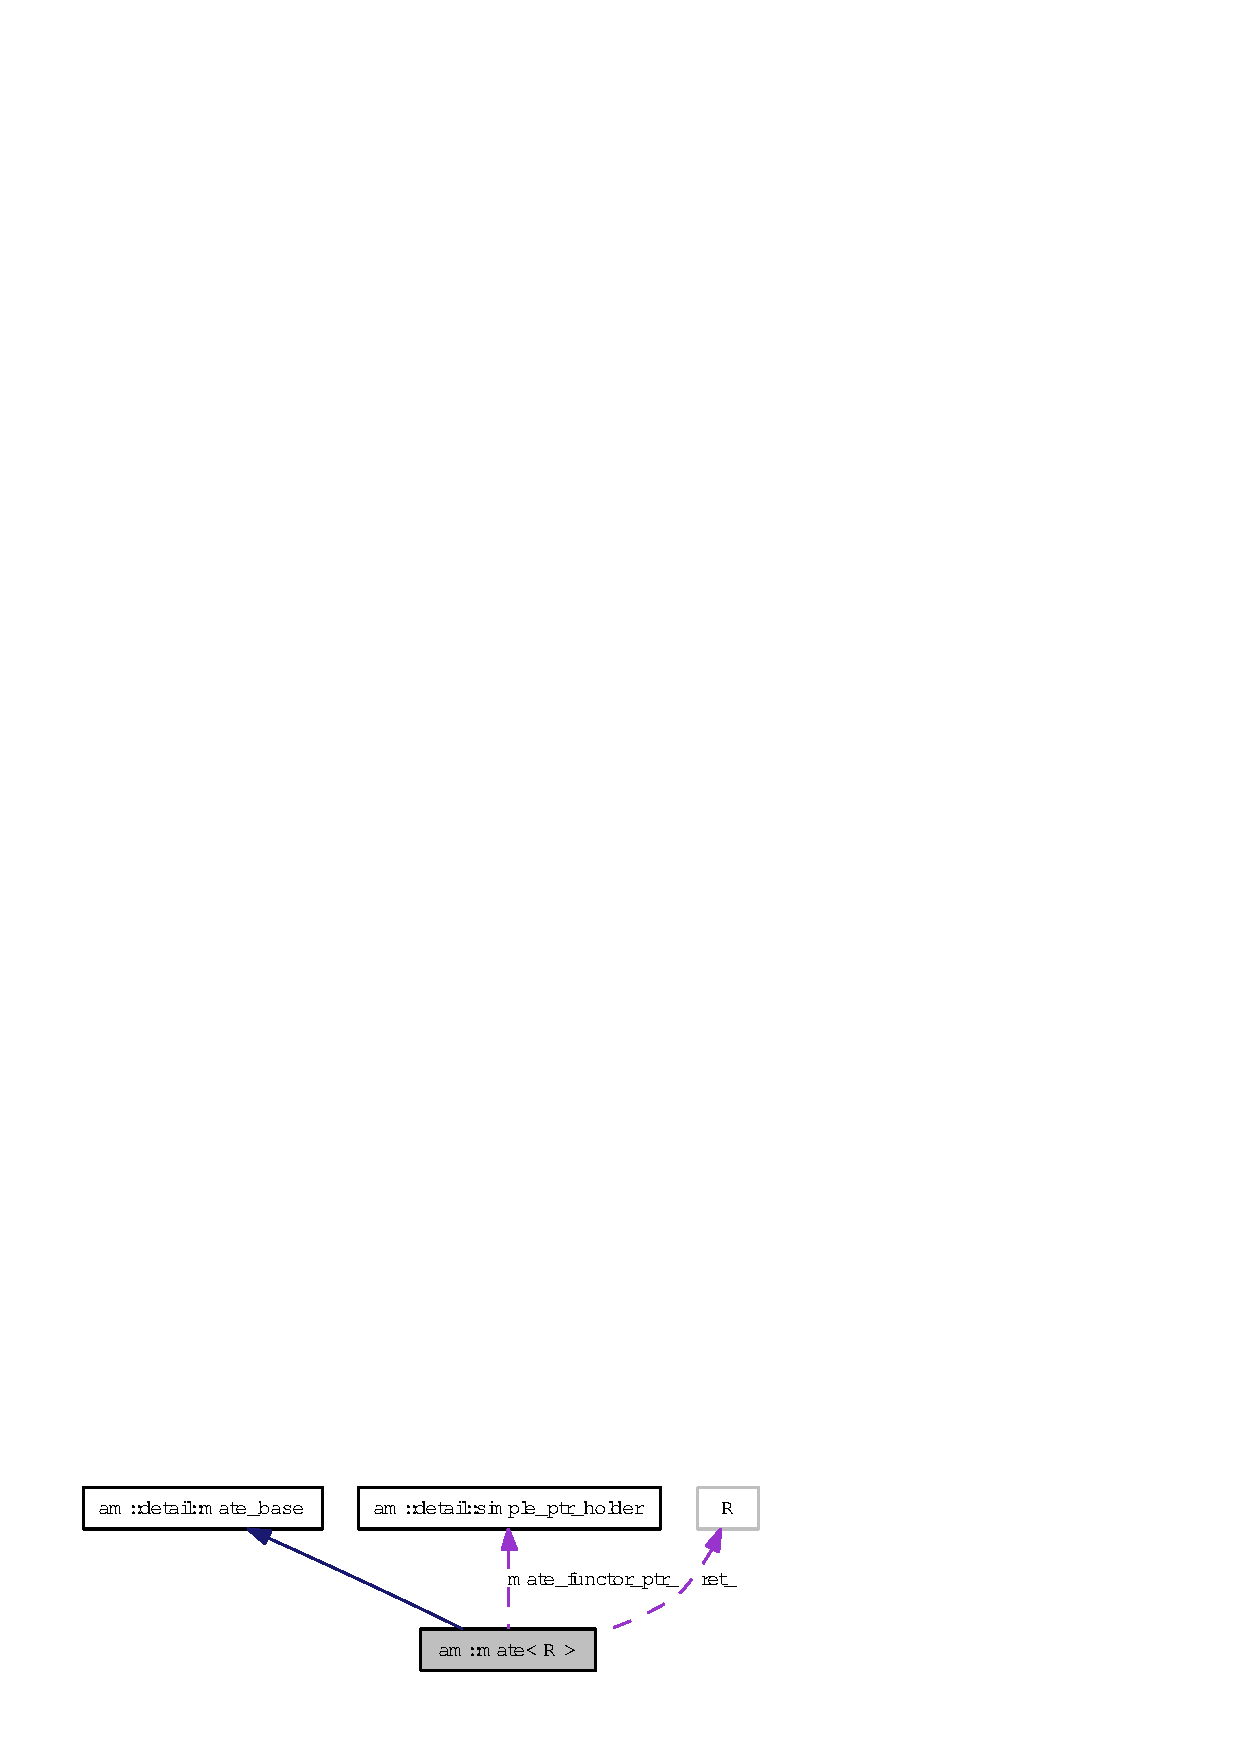
\includegraphics[width=185pt]{classam_1_1mate__coll__graph}
\end{center}
\end{figure}
\subsection*{Public Member Functions}
\begin{CompactItemize}
\item 
template$<$class T$>$ {\bf mate} (R ret, T mate\_\-functor)
\item 
template$<$class T, class C$>$ {\bf mate} (R ret, T mate\_\-functor, C mate\_\-if)
\item 
{\bf $\sim$mate} ()
\item 
void {\bf run\_\-mate} (bool delete\_\-mate\_\-now=false)
\item 
void {\bf dismiss\_\-mate} (bool delete\_\-mate\_\-now=false)
\item 
{\bf operator R} () const
\end{CompactItemize}
\subsection*{Private Types}
\begin{CompactItemize}
\item 
typedef void($\ast$) \textbf{typeless\_\-mate\_\-stub} (void $\ast$, R)\label{classam_1_1mate_ee9347452cd87f7f0fc174ee8eece9de}

\end{CompactItemize}
\subsection*{Private Member Functions}
\begin{CompactItemize}
\item 
{\bf mate}$<$ R $>$ \& {\bf operator=} ({\bf mate}$<$ R $>$ const \&)\label{classam_1_1mate_a2cffaf7bd7a21ba6671e3eb7b7290be}

\begin{CompactList}\small\item\em Restrict assignment. \item\end{CompactList}\end{CompactItemize}
\subsection*{Private Attributes}
\begin{CompactItemize}
\item 
R {\bf ret\_\-}\label{classam_1_1mate_96d8f086acedaaba49fa8dda704c6e68}

\begin{CompactList}\small\item\em Return of the host function. \item\end{CompactList}\item 
{\bf detail::simple\_\-ptr\_\-holder} {\bf mate\_\-functor\_\-ptr\_\-}\label{classam_1_1mate_dac8b8d494662bc0c5cf0a9f0586a465}

\begin{CompactList}\small\item\em Mate functoion object. \item\end{CompactList}\item 
typeless\_\-mate\_\-stub {\bf mate\_\-stub\_\-}\label{classam_1_1mate_72f5837ec74e2e14cdb93f69031b95be}

\begin{CompactList}\small\item\em Typeless mate function object invoker. \item\end{CompactList}\end{CompactItemize}
\subsection*{Classes}
\begin{CompactItemize}
\item 
struct {\bf typed\_\-}
\end{CompactItemize}


\subsection{Detailed Description}
\subsubsection*{template$<$class R$>$ class am::mate$<$ R $>$}

Mates a host function with the mate function object. 

Mates (associates) the result of the host function with the mate function object so that the associated mate function object is called int its destructor automatically when it goes out of scope. 



\subsection{Constructor \& Destructor Documentation}
\index{am::mate@{am::mate}!mate@{mate}}
\index{mate@{mate}!am::mate@{am::mate}}
\subsubsection{\setlength{\rightskip}{0pt plus 5cm}template$<$class R$>$ template$<$class T$>$ {\bf am::mate}$<$ R $>$::{\bf mate} (R {\em ret}, T {\em mate\_\-functor})\hspace{0.3cm}{\tt  [inline]}}\label{classam_1_1mate_52e89c5bf178aff995128a241fc6c3cc}


Constructor.

\begin{Desc}
\item[Parameters:]
\begin{description}
\item[\mbox{$\leftarrow$} {\em ret}]Specifies the return of the host function. \item[\mbox{$\leftarrow$} {\em mate\_\-functor}]Specifies the mate function object which will be called in the destructor. It should be a unary function object which accept {\em ret\/} as its argument.\end{description}
\end{Desc}
\begin{Desc}
\item[Precondition:]Host function should not throw an exception. \end{Desc}
\index{am::mate@{am::mate}!mate@{mate}}
\index{mate@{mate}!am::mate@{am::mate}}
\subsubsection{\setlength{\rightskip}{0pt plus 5cm}template$<$class R$>$ template$<$class T, class C$>$ {\bf am::mate}$<$ R $>$::{\bf mate} (R {\em ret}, T {\em mate\_\-functor}, C {\em mate\_\-if})\hspace{0.3cm}{\tt  [inline]}}\label{classam_1_1mate_0992eeb490ba954833e27e0935861b5a}


Constructor.

\begin{Desc}
\item[Parameters:]
\begin{description}
\item[\mbox{$\leftarrow$} {\em ret}]Specifies the return of the host function. \item[\mbox{$\leftarrow$} {\em mate\_\-functor}]Specifies the mate function object which will be called in the destructor. It should be an unary function object which accept {\em ret\/} as its argument. \item[\mbox{$\leftarrow$} {\em mate\_\-if}]Specifies the predicate which determines whether or not the specified mate function object will be called in the destructor. It should be an unary predicate which accept {\em ret\/} as its argument. If it return false, no heap memory allocation is even occurred to store the mate function object.\end{description}
\end{Desc}
\begin{Desc}
\item[Precondition:]Host function should not throw an exception. \end{Desc}
\index{am::mate@{am::mate}!~mate@{$\sim$mate}}
\index{~mate@{$\sim$mate}!am::mate@{am::mate}}
\subsubsection{\setlength{\rightskip}{0pt plus 5cm}template$<$class R$>$ {\bf am::mate}$<$ R $>$::$\sim${\bf mate} ()\hspace{0.3cm}{\tt  [inline]}}\label{classam_1_1mate_29cac99d41b0fb1cbd0be3e2c841444c}


Destructor. Calls mate function object. 

\subsection{Member Function Documentation}
\index{am::mate@{am::mate}!run_mate@{run\_\-mate}}
\index{run_mate@{run\_\-mate}!am::mate@{am::mate}}
\subsubsection{\setlength{\rightskip}{0pt plus 5cm}template$<$class R$>$ void {\bf am::mate}$<$ R $>$::run\_\-mate (bool {\em delete\_\-mate\_\-now} = {\tt false})\hspace{0.3cm}{\tt  [inline]}}\label{classam_1_1mate_93fe5fc5abbe71780e7638bde72e1845}


Run mate function object now.

\begin{Desc}
\item[Parameters:]
\begin{description}
\item[\mbox{$\leftarrow$} {\em delete\_\-mate\_\-now}]Specifies whether or not the mate function object will be deallocated after calling the mate function object. If false, the mate function object will be deallocated in the destructor when it goes out of scope. \end{description}
\end{Desc}
\begin{Desc}
\item[Returns:]void. \end{Desc}
\index{am::mate@{am::mate}!dismiss_mate@{dismiss\_\-mate}}
\index{dismiss_mate@{dismiss\_\-mate}!am::mate@{am::mate}}
\subsubsection{\setlength{\rightskip}{0pt plus 5cm}template$<$class R$>$ void {\bf am::mate}$<$ R $>$::dismiss\_\-mate (bool {\em delete\_\-mate\_\-now} = {\tt false})\hspace{0.3cm}{\tt  [inline]}}\label{classam_1_1mate_2ecbeb01954567c013e9322aa5e8e0da}


Dismiss the mate functor.

\begin{Desc}
\item[Parameters:]
\begin{description}
\item[\mbox{$\leftarrow$} {\em delete\_\-mate\_\-now}]Specifies whether or not the mate function object will be deallocated. If false, the mate function object will be deallocated in the destructor when it goes out of scope. \end{description}
\end{Desc}
\begin{Desc}
\item[Returns:]void. \end{Desc}
\index{am::mate@{am::mate}!operator R@{operator R}}
\index{operator R@{operator R}!am::mate@{am::mate}}
\subsubsection{\setlength{\rightskip}{0pt plus 5cm}template$<$class R$>$ {\bf am::mate}$<$ R $>$::operator R () const\hspace{0.3cm}{\tt  [inline]}}\label{classam_1_1mate_5bd50a39a4ed2ee277652d394de0acab}


Implicit conversion. Cast an illusion to make it possible to use a mate instance as if it is a raw variable stored, which is the return of the host function.

\begin{Desc}
\item[Returns:]Copy of the stored raw variable, which is the return of the host function. \end{Desc}


The documentation for this class was generated from the following file:\begin{CompactItemize}
\item 
{\bf mate.hpp}\end{CompactItemize}

\section{am::mate$<$ R $>$::typed\_\-$<$ T $>$ Struct Template Reference}
\label{structam_1_1mate_1_1typed__}\index{am::mate::typed_@{am::mate::typed\_\-}}
\subsection*{Static Public Member Functions}
\begin{CompactItemize}
\item 
static void {\bf mate\_\-stub} (void $\ast$mate\_\-ptr, R ret)
\end{CompactItemize}


\subsection{Detailed Description}
\subsubsection*{template$<$class R$>$template$<$class T$>$ struct am::mate$<$ R $>$::typed\_\-$<$ T $>$}

\begin{Desc}
\item[For internal use only.]
typed mate function object mfn\_\-invoker stub. \end{Desc}




\subsection{Member Function Documentation}
\index{am::mate::typed_@{am::mate::typed\_\-}!mate_stub@{mate\_\-stub}}
\index{mate_stub@{mate\_\-stub}!am::mate::typed_@{am::mate::typed\_\-}}
\subsubsection{\setlength{\rightskip}{0pt plus 5cm}template$<$class R$>$ template$<$class T$>$ static void {\bf am::mate}$<$ R $>$::{\bf typed\_\-}$<$ T $>$::mate\_\-stub (void $\ast$ {\em mate\_\-ptr}, R {\em ret})\hspace{0.3cm}{\tt  [inline, static]}}\label{structam_1_1mate_1_1typed___604d3e830773c811354ba20ad1b0ec2f}


Invoke the mate function object in type safe manner.

\begin{Desc}
\item[Parameters:]
\begin{description}
\item[\mbox{$\leftarrow$} {\em mate\_\-ptr}]Specifies typeless mate function object. \item[\mbox{$\leftarrow$} {\em ret}]Specifies the return of the host function. \end{description}
\end{Desc}
\begin{Desc}
\item[Returns:]void. \end{Desc}


The documentation for this struct was generated from the following file:\begin{CompactItemize}
\item 
{\bf mate.hpp}\end{CompactItemize}

\section{am::mate$<$ void $>$ Class Template Reference}
\label{classam_1_1mate_3_01void_01_4}\index{am::mate< void >@{am::mate$<$ void $>$}}
void template specialization for mate.  


{\tt \#include $<$mate.hpp$>$}

Collaboration diagram for am::mate$<$ void $>$:\begin{figure}[H]
\begin{center}
\leavevmode
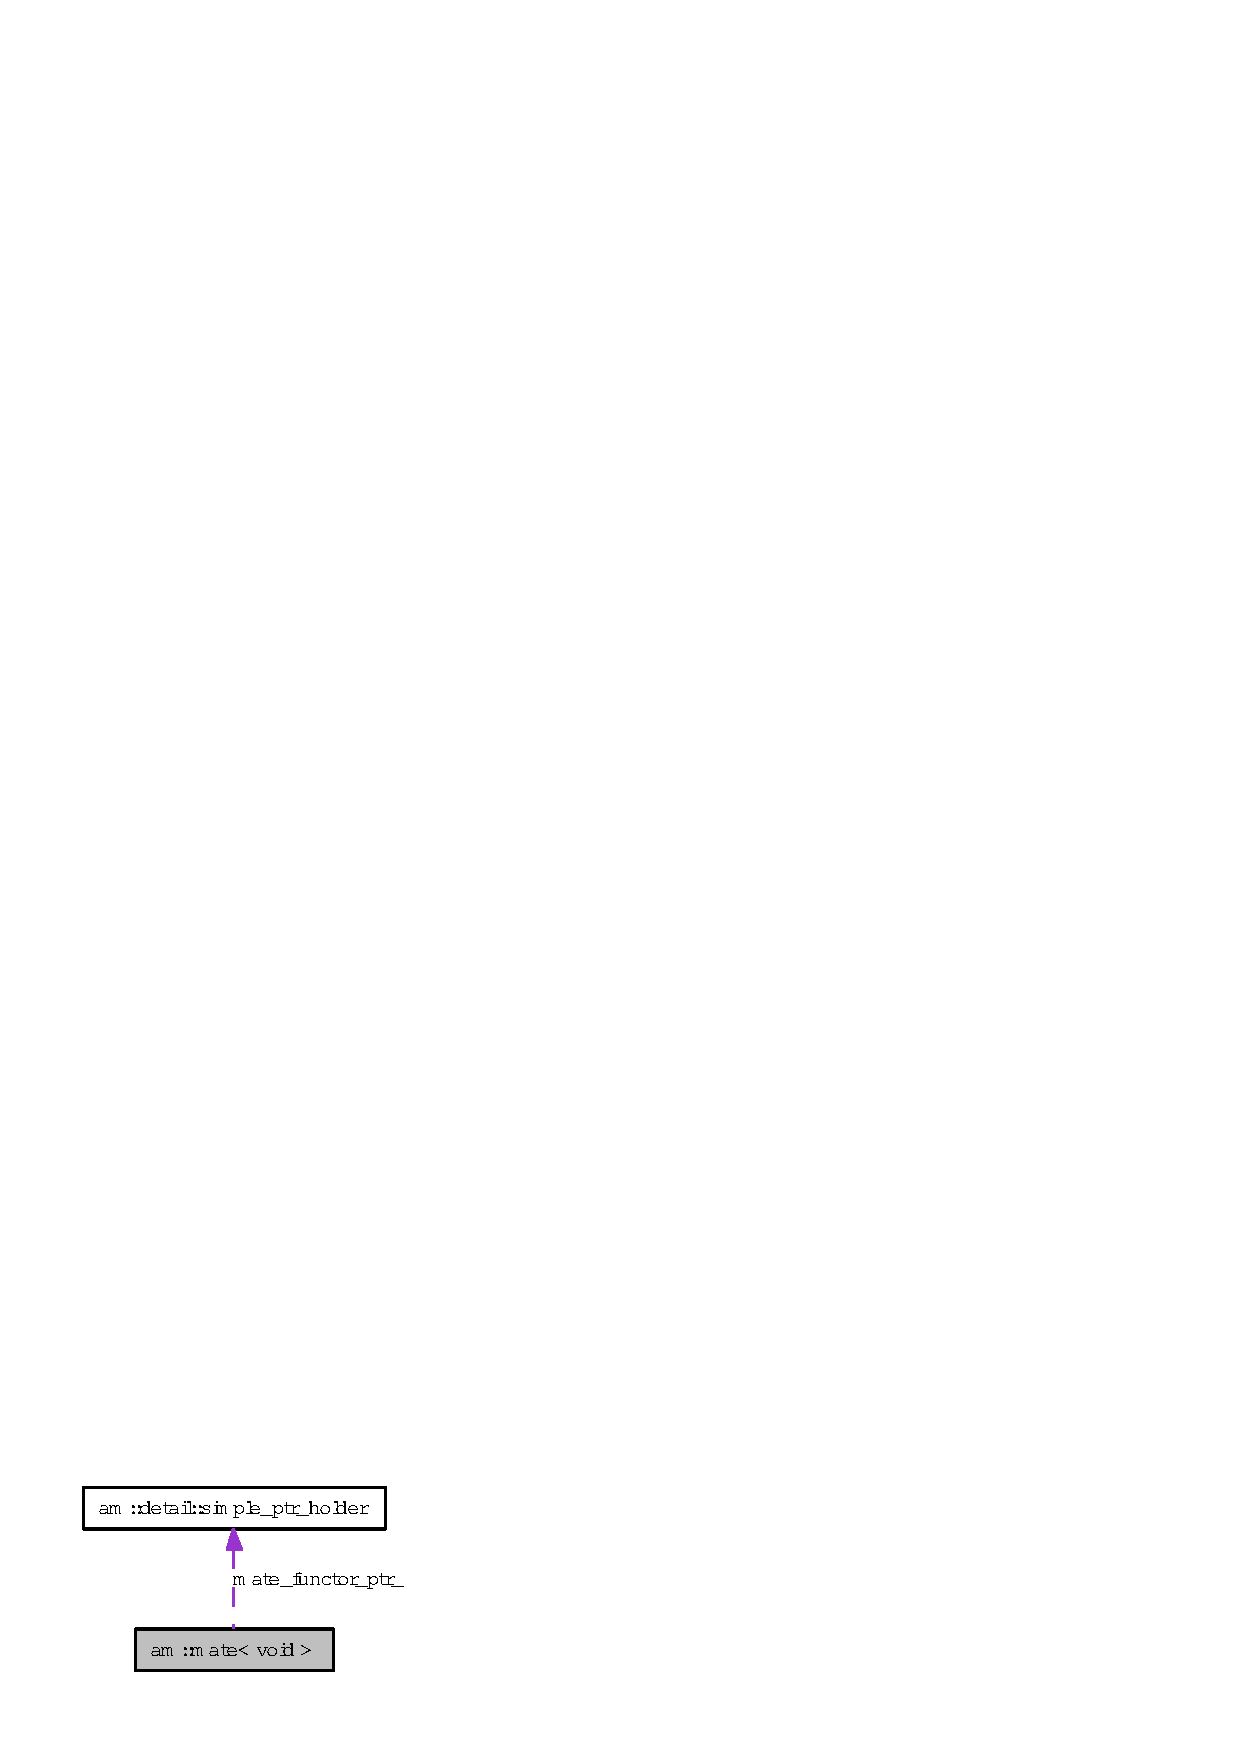
\includegraphics[width=99pt]{classam_1_1mate_3_01void_01_4__coll__graph}
\end{center}
\end{figure}
\subsection*{Public Member Functions}
\begin{CompactItemize}
\item 
template$<$class T$>$ {\bf mate} (T mate\_\-functor)
\item 
template$<$class T, class C$>$ {\bf mate} (T mate\_\-functor, C mate\_\-if)
\item 
{\bf $\sim$mate} ()
\item 
void {\bf run\_\-mate} (bool delete\_\-mate\_\-now=false)
\item 
void {\bf dismiss\_\-mate} (bool delete\_\-mate\_\-now=false)
\end{CompactItemize}
\subsection*{Private Types}
\begin{CompactItemize}
\item 
typedef void($\ast$) \textbf{typeless\_\-mate\_\-stub} (void $\ast$)\label{classam_1_1mate_3_01void_01_4_a9355418db2898e3ece0e478f04c99b6}

\end{CompactItemize}
\subsection*{Private Member Functions}
\begin{CompactItemize}
\item 
{\bf mate}$<$ void $>$ \& {\bf operator=} ({\bf mate}$<$ void $>$ const \&)\label{classam_1_1mate_3_01void_01_4_54f6fc23d1d5107b7ed42e0f9dd80d7d}

\begin{CompactList}\small\item\em Restrict assignment. \item\end{CompactList}\end{CompactItemize}
\subsection*{Private Attributes}
\begin{CompactItemize}
\item 
{\bf detail::simple\_\-ptr\_\-holder} {\bf mate\_\-functor\_\-ptr\_\-}\label{classam_1_1mate_3_01void_01_4_547feb6a6535470c1d1b2d6e2aa1d5cb}

\begin{CompactList}\small\item\em Mate function object. \item\end{CompactList}\item 
typeless\_\-mate\_\-stub {\bf mate\_\-stub\_\-}\label{classam_1_1mate_3_01void_01_4_470f0f0b07bc81985ddf4a91158d5d88}

\begin{CompactList}\small\item\em Typeless mate function object invoker. \item\end{CompactList}\end{CompactItemize}
\subsection*{Classes}
\begin{CompactItemize}
\item 
struct {\bf typed\_\-}
\end{CompactItemize}


\subsection{Detailed Description}
\subsubsection*{template$<$$>$ class am::mate$<$ void $>$}

void template specialization for mate. 

Specifies mate function object to be called in its destructor automatically when it goes out of scope.

\begin{Desc}
\item[See also:]\doxyref{MATE\_\-VOID()}{p.}{mate_8hpp_b64fb21cccc9097c72ddab9f2c37d78a}, \doxyref{MATE\_\-VOID\_\-IF()}{p.}{mate_8hpp_becd3ca3f114b18666fd383aad100fef} \end{Desc}




\subsection{Constructor \& Destructor Documentation}
\index{am::mate< void >@{am::mate$<$ void $>$}!mate@{mate}}
\index{mate@{mate}!am::mate< void >@{am::mate$<$ void $>$}}
\subsubsection{\setlength{\rightskip}{0pt plus 5cm}template$<$class T$>$ {\bf am::mate}$<$ void $>$::{\bf mate} (T {\em mate\_\-functor})\hspace{0.3cm}{\tt  [inline]}}\label{classam_1_1mate_3_01void_01_4_ef870d95333a39703bce1fa30f8b1366}


Constructor.

\begin{Desc}
\item[Parameters:]
\begin{description}
\item[\mbox{$\leftarrow$} {\em mate\_\-functor}]Specifies the mate function object which will be called in the destructor. It should be a null-nary function object which does not accept any argument. \end{description}
\end{Desc}
\index{am::mate< void >@{am::mate$<$ void $>$}!mate@{mate}}
\index{mate@{mate}!am::mate< void >@{am::mate$<$ void $>$}}
\subsubsection{\setlength{\rightskip}{0pt plus 5cm}template$<$class T, class C$>$ {\bf am::mate}$<$ void $>$::{\bf mate} (T {\em mate\_\-functor}, C {\em mate\_\-if})\hspace{0.3cm}{\tt  [inline]}}\label{classam_1_1mate_3_01void_01_4_1b8b737f7cd16feb8dbb7a2ded92a2f0}


Constructor.

\begin{Desc}
\item[Parameters:]
\begin{description}
\item[\mbox{$\leftarrow$} {\em mate\_\-functor}]Specifies the mate function object which will be called in the destructor. It should be an null-nary function object which does not accept any argument. \item[\mbox{$\leftarrow$} {\em mate\_\-if}]Specifies the predicate which determines whether or not the specified mate function object will be called in the destructor. It should be an null-nary predicate which does not accept any argument. If it return false, no heap memory allocation is even occurred to store the mate function object. \end{description}
\end{Desc}
\index{am::mate< void >@{am::mate$<$ void $>$}!~mate@{$\sim$mate}}
\index{~mate@{$\sim$mate}!am::mate< void >@{am::mate$<$ void $>$}}
\subsubsection{\setlength{\rightskip}{0pt plus 5cm}{\bf am::mate}$<$ void $>$::$\sim${\bf mate} ()\hspace{0.3cm}{\tt  [inline]}}\label{classam_1_1mate_3_01void_01_4_8a09874d12772b460169cf917b4cdefe}


Destructor. Calls mate function object. 

\subsection{Member Function Documentation}
\index{am::mate< void >@{am::mate$<$ void $>$}!run_mate@{run\_\-mate}}
\index{run_mate@{run\_\-mate}!am::mate< void >@{am::mate$<$ void $>$}}
\subsubsection{\setlength{\rightskip}{0pt plus 5cm}void {\bf am::mate}$<$ void $>$::run\_\-mate (bool {\em delete\_\-mate\_\-now} = {\tt false})\hspace{0.3cm}{\tt  [inline]}}\label{classam_1_1mate_3_01void_01_4_4bfa3850f558f7398e7fe3f44746a848}


Run mate function object now.

\begin{Desc}
\item[Parameters:]
\begin{description}
\item[\mbox{$\leftarrow$} {\em delete\_\-mate\_\-now}]Specifies whether or not the mate function object will be deallocated after calling the mate function object. If false, the mate function object will be deallocated in the destructor when it goes out of scope. \end{description}
\end{Desc}
\begin{Desc}
\item[Returns:]void. \end{Desc}
\index{am::mate< void >@{am::mate$<$ void $>$}!dismiss_mate@{dismiss\_\-mate}}
\index{dismiss_mate@{dismiss\_\-mate}!am::mate< void >@{am::mate$<$ void $>$}}
\subsubsection{\setlength{\rightskip}{0pt plus 5cm}void {\bf am::mate}$<$ void $>$::dismiss\_\-mate (bool {\em delete\_\-mate\_\-now} = {\tt false})\hspace{0.3cm}{\tt  [inline]}}\label{classam_1_1mate_3_01void_01_4_8eb3e9530f85a64c484473b1f7358565}


Dismiss the mate function object.

\begin{Desc}
\item[Parameters:]
\begin{description}
\item[\mbox{$\leftarrow$} {\em delete\_\-mate\_\-now}]Specifies whether or not the mate function object will be deallocated. If false, the mate function object will be deallocated in the destructor when it goes out of scope. \end{description}
\end{Desc}
\begin{Desc}
\item[Returns:]void. \end{Desc}


The documentation for this class was generated from the following file:\begin{CompactItemize}
\item 
{\bf mate.hpp}\end{CompactItemize}

\section{am::mate$<$ void $>$::typed\_\-$<$ T $>$ Struct Template Reference}
\label{structam_1_1mate_3_01void_01_4_1_1typed__}\index{am::mate< void >::typed_@{am::mate$<$ void $>$::typed\_\-}}
\subsection*{Static Public Member Functions}
\begin{CompactItemize}
\item 
static void {\bf mate\_\-stub} (void $\ast$mate\_\-ptr)
\end{CompactItemize}


\subsection{Detailed Description}
\subsubsection*{template$<$$>$template$<$class T$>$ struct am::mate$<$ void $>$::typed\_\-$<$ T $>$}

\begin{Desc}
\item[For internal use only.]
typed mate function object mfn\_\-invoker stub. \end{Desc}




\subsection{Member Function Documentation}
\index{am::mate< void >::typed_@{am::mate$<$ void $>$::typed\_\-}!mate_stub@{mate\_\-stub}}
\index{mate_stub@{mate\_\-stub}!am::mate< void >::typed_@{am::mate$<$ void $>$::typed\_\-}}
\subsubsection{\setlength{\rightskip}{0pt plus 5cm}template$<$class T$>$ static void {\bf am::mate}$<$ void $>$::typed\_\-$<$ T $>$::mate\_\-stub (void $\ast$ {\em mate\_\-ptr})\hspace{0.3cm}{\tt  [inline, static]}}\label{structam_1_1mate_3_01void_01_4_1_1typed___8346c15870f9a2d06f5acf1d0abd63ba}


Invoke the mate function object in type safe manner.

\begin{Desc}
\item[Parameters:]
\begin{description}
\item[\mbox{$\leftarrow$} {\em mate\_\-ptr}]Specifies typeless mate function object. \end{description}
\end{Desc}
\begin{Desc}
\item[Returns:]void. \end{Desc}


The documentation for this struct was generated from the following file:\begin{CompactItemize}
\item 
{\bf mate.hpp}\end{CompactItemize}

\section{am::detail::mate\_\-base Class Reference}
\label{classam_1_1detail_1_1mate__base}\index{am::detail::mate_base@{am::detail::mate\_\-base}}
{\tt \#include $<$mate.hpp$>$}

Inherited by {\bf am::mate$<$ R $>$}.

Inheritance diagram for am::detail::mate\_\-base:\begin{figure}[H]
\begin{center}
\leavevmode
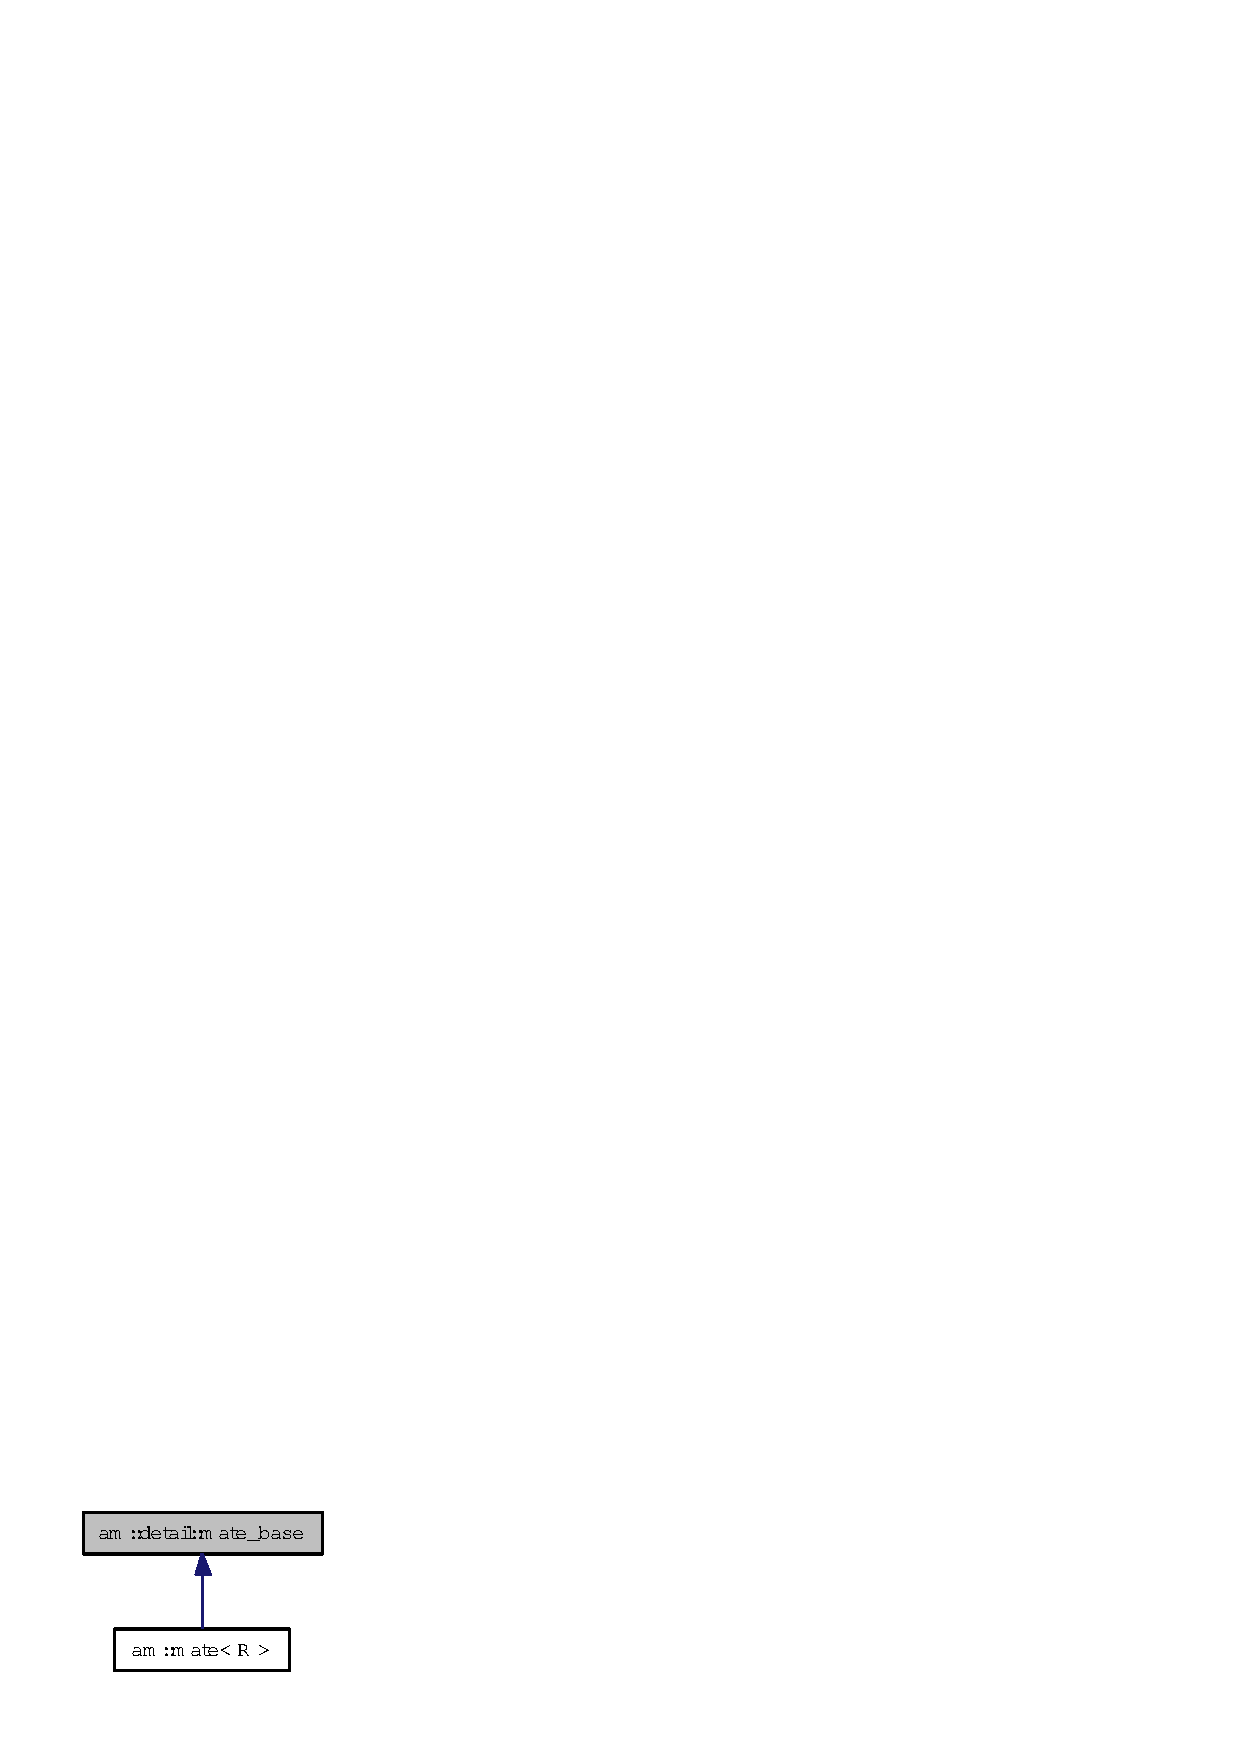
\includegraphics[width=79pt]{classam_1_1detail_1_1mate__base__inherit__graph}
\end{center}
\end{figure}


\subsection{Detailed Description}
\begin{Desc}
\item[For internal use only.]
Base class of mate

\begin{Desc}
\item[See also:]\doxyref{AM\_\-ANONYMOUS\_\-MATE()}{p.}{mate_8hpp_0b43846b9d4b2cf0017afdb28a0fdda6}, \doxyref{AM\_\-ANONYMOUS\_\-MATE\_\-IF()}{p.}{mate_8hpp_a986ab16c039b02db09e4da015c65a0d} \end{Desc}
\end{Desc}




The documentation for this class was generated from the following file:\begin{CompactItemize}
\item 
{\bf mate.hpp}\end{CompactItemize}

\section{am::lambda::pf\_\-memdata$<$ P, O, U $>$ Struct Template Reference}
\label{structam_1_1lambda_1_1pf__memdata}\index{am::lambda::pf_memdata@{am::lambda::pf\_\-memdata}}
{\tt \#include $<$lambda.hpp$>$}

Inherits {\bf am::lambda::detail::lambda\_\-op\_\-tag}.

Inheritance diagram for am::lambda::pf\_\-memdata$<$ P, O, U $>$:\begin{figure}[H]
\begin{center}
\leavevmode
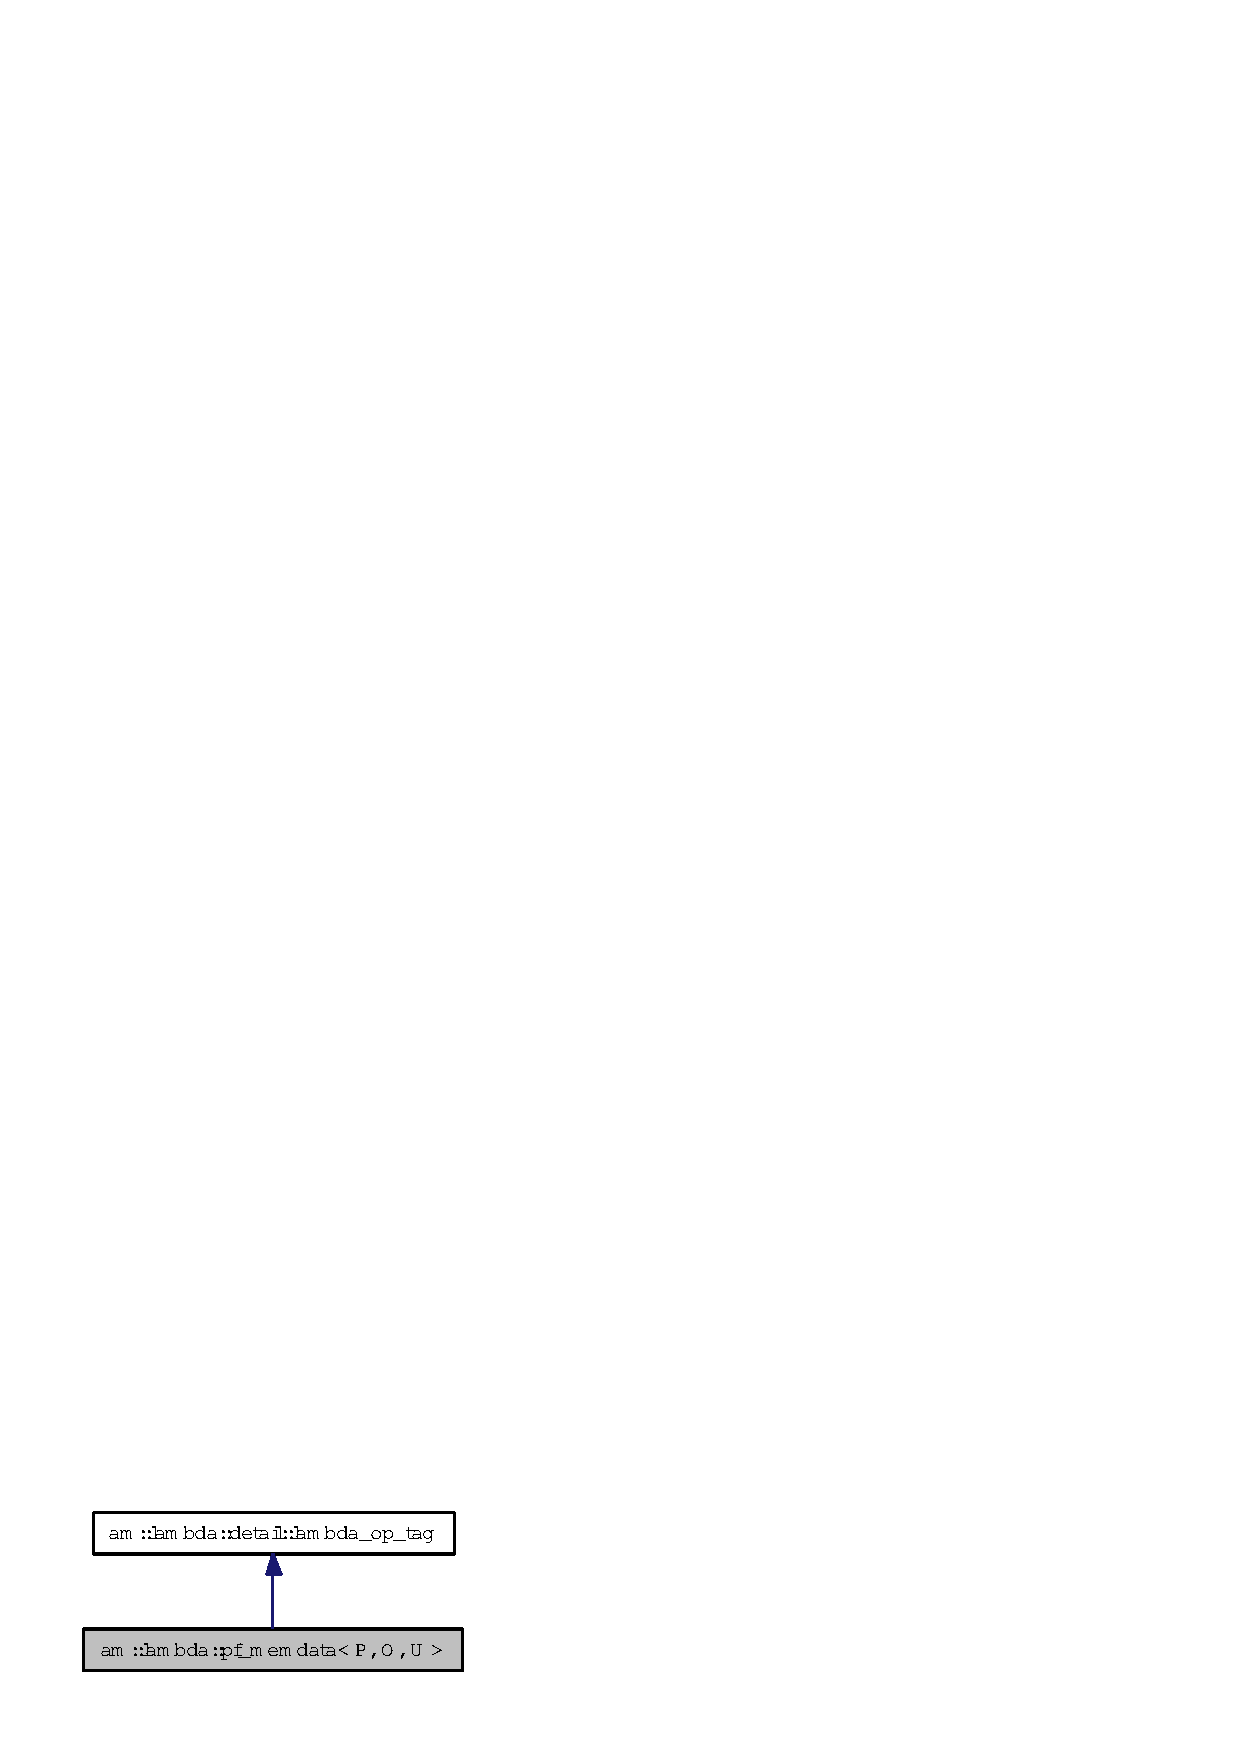
\includegraphics[width=113pt]{structam_1_1lambda_1_1pf__memdata__inherit__graph}
\end{center}
\end{figure}
Collaboration diagram for am::lambda::pf\_\-memdata$<$ P, O, U $>$:\begin{figure}[H]
\begin{center}
\leavevmode
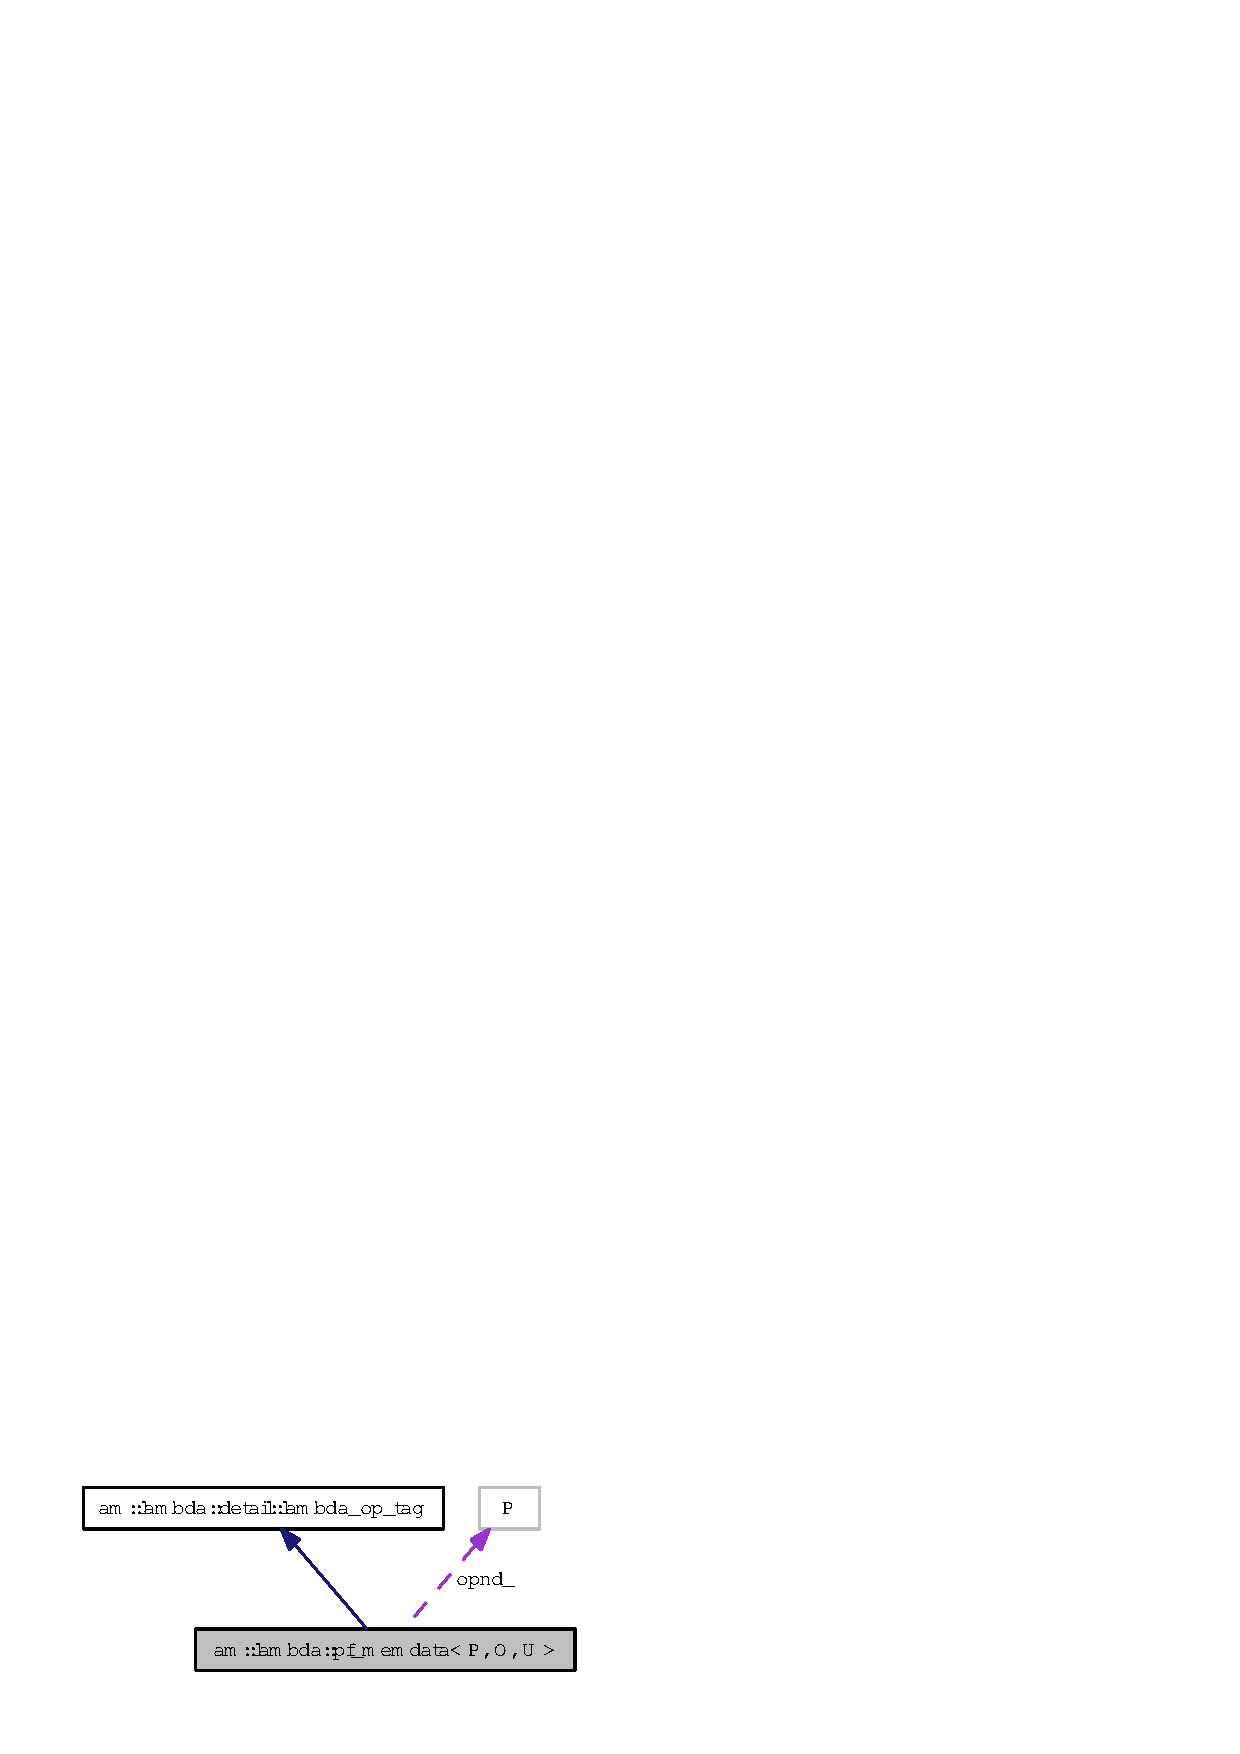
\includegraphics[width=140pt]{structam_1_1lambda_1_1pf__memdata__coll__graph}
\end{center}
\end{figure}
\subsection*{Public Member Functions}
\begin{CompactItemize}
\item 
\textbf{pf\_\-memdata} (P opnd, U(O::$\ast$pu))\label{structam_1_1lambda_1_1pf__memdata_9fe96a12a227ed71cc1b0726116c8fb3}

\item 
template$<$class T1, class T2, class T3$>$ U const \& \textbf{operator()} (T1 \&t1, T2 \&t2, T3 \&t3) const \label{structam_1_1lambda_1_1pf__memdata_b40e1eefad6d26a955ffb4cc82434650}

\item 
template$<$class T1, class T2$>$ U const \& \textbf{operator()} (T1 \&t1, T2 \&t2) const \label{structam_1_1lambda_1_1pf__memdata_c6274e3380a83ffe6b2d96e1a36ddb68}

\item 
template$<$class T1$>$ U const \& \textbf{operator()} (T1 \&t1) const\label{structam_1_1lambda_1_1pf__memdata_60d1c08701f9c711ce5cbf8b505e5efe}

\item 
{\bf address\_\-of} \textbf{operator \&} () const\label{structam_1_1lambda_1_1pf__memdata_860bb00118c6f6147c231a62eaa50fcd}

\end{CompactItemize}
\subsection*{Public Attributes}
\begin{CompactItemize}
\item 
P \textbf{opnd\_\-}\label{structam_1_1lambda_1_1pf__memdata_9cff67d816aefbe768f8d72ff882db4b}

\item 
UO::$\ast$ \textbf{pu\_\-}\label{structam_1_1lambda_1_1pf__memdata_a44cac02967ca15bd8efaa831454e5d6}

\end{CompactItemize}
\subsection*{Classes}
\begin{CompactItemize}
\item 
struct {\bf address\_\-of}
\end{CompactItemize}


\subsection{Detailed Description}
\subsubsection*{template$<$class P, class O, class U$>$ struct am::lambda::pf\_\-memdata$<$ P, O, U $>$}

\begin{Desc}
\item[For internal use only.]
Pure Function to support member data pointer access. \end{Desc}




The documentation for this struct was generated from the following file:\begin{CompactItemize}
\item 
{\bf lambda.hpp}\end{CompactItemize}

\section{am::lambda::pf\_\-memdata$<$ P, O, U $>$::address\_\-of Struct Reference}
\label{structam_1_1lambda_1_1pf__memdata_1_1address__of}\index{am::lambda::pf_memdata::address_of@{am::lambda::pf\_\-memdata::address\_\-of}}
{\tt \#include $<$lambda.hpp$>$}

Inherits {\bf am::lambda::detail::lambda\_\-op\_\-tag}.

Inheritance diagram for am::lambda::pf\_\-memdata$<$ P, O, U $>$::address\_\-of:\begin{figure}[H]
\begin{center}
\leavevmode
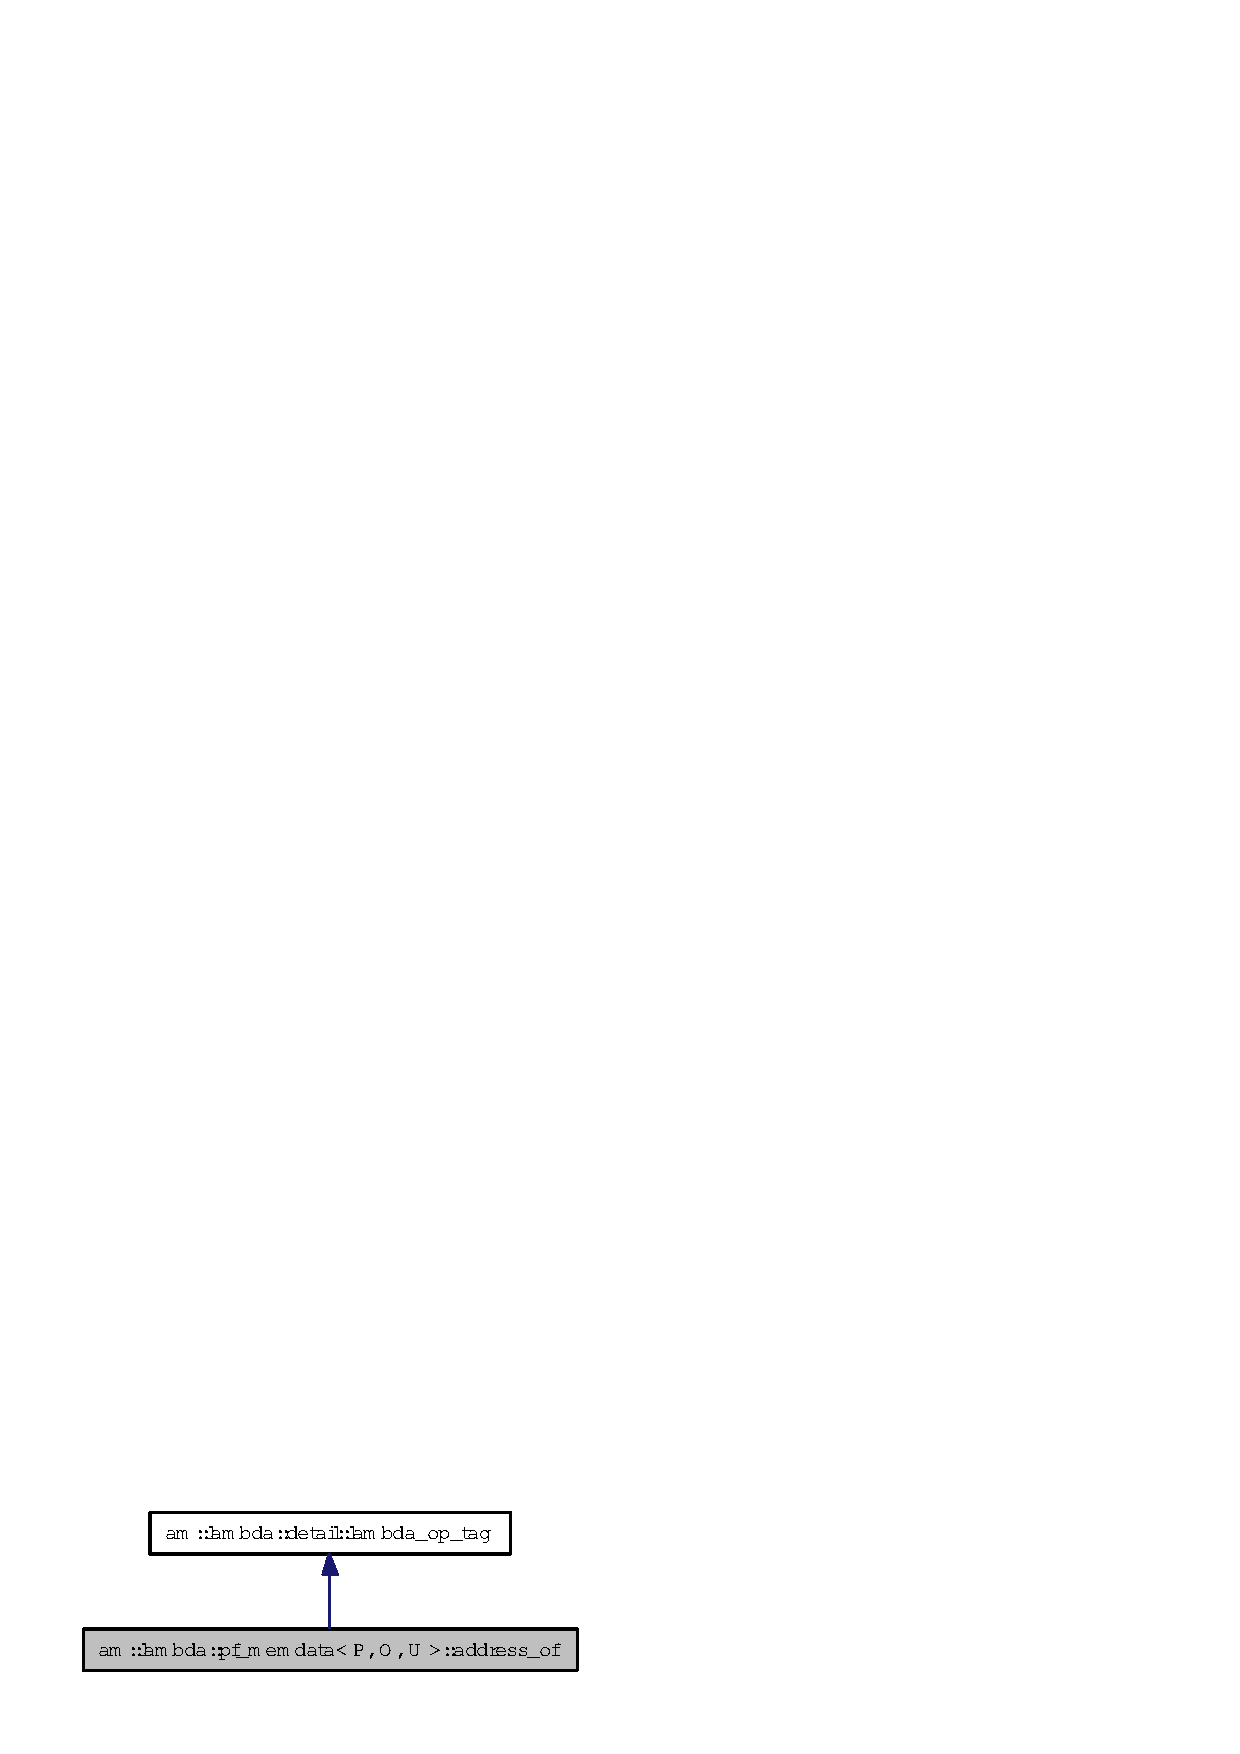
\includegraphics[width=140pt]{structam_1_1lambda_1_1pf__memdata_1_1address__of__inherit__graph}
\end{center}
\end{figure}
Collaboration diagram for am::lambda::pf\_\-memdata$<$ P, O, U $>$::address\_\-of:\begin{figure}[H]
\begin{center}
\leavevmode
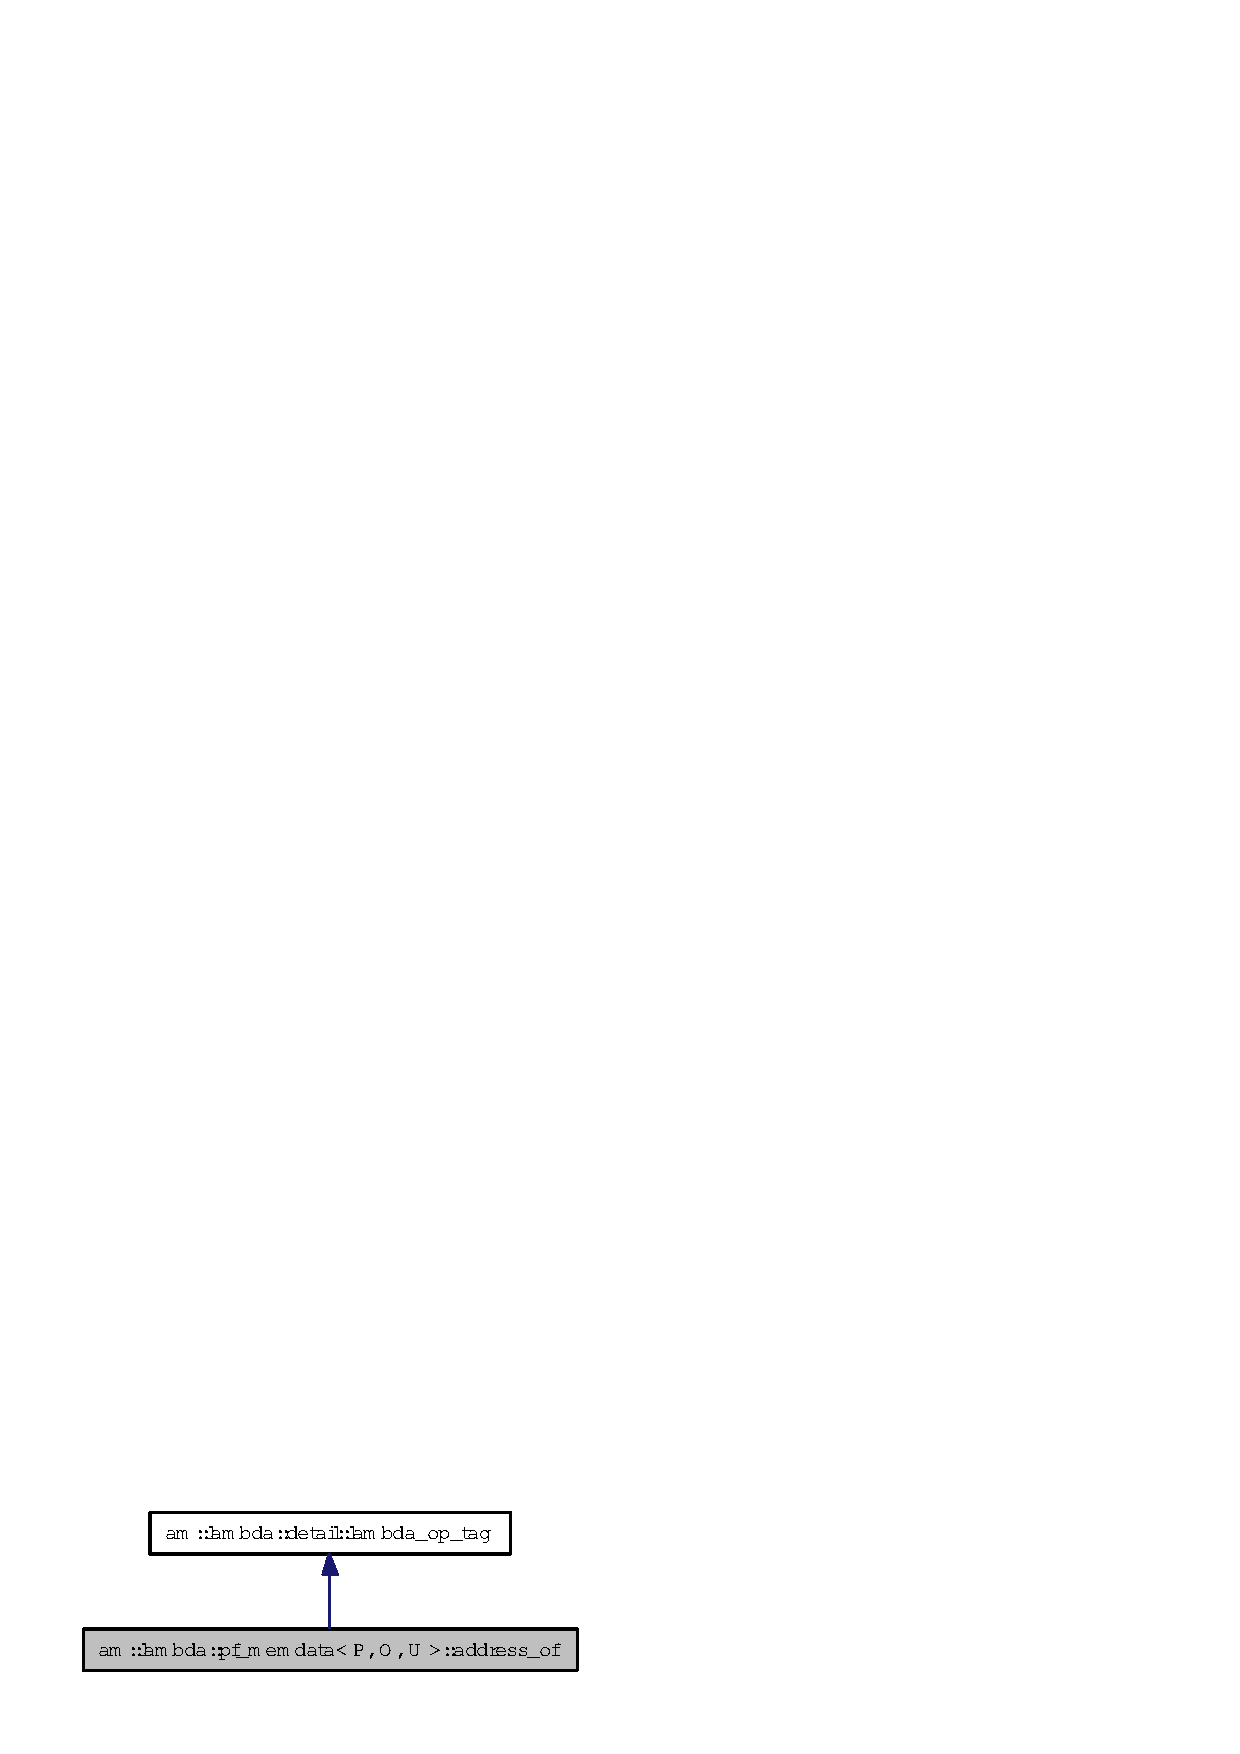
\includegraphics[width=140pt]{structam_1_1lambda_1_1pf__memdata_1_1address__of__coll__graph}
\end{center}
\end{figure}
\subsection*{Public Member Functions}
\begin{CompactItemize}
\item 
\textbf{address\_\-of} ({\bf pf\_\-memdata}$<$ P, O, U $>$ const \&pmd)\label{structam_1_1lambda_1_1pf__memdata_1_1address__of_c26aa71a1ffdf4f63e9c2bdd26648226}

\item 
template$<$class T1, class T2, class T3$>$ U const $\ast$ \textbf{operator()} (T1 \&t1, T2 \&t2, T3 \&t3) const \label{structam_1_1lambda_1_1pf__memdata_1_1address__of_8b3c885c123ccd9c8b7432a22cf5d2d2}

\item 
template$<$class T1, class T2$>$ U const $\ast$ \textbf{operator()} (T1 \&t1, T2 \&t2) const \label{structam_1_1lambda_1_1pf__memdata_1_1address__of_739a5375d13740ac5c782f8ad68c1c9d}

\item 
template$<$class T1$>$ U const $\ast$ \textbf{operator()} (T1 \&t1) const\label{structam_1_1lambda_1_1pf__memdata_1_1address__of_9639284f5192ec6b8a1385b1d379e15a}

\end{CompactItemize}
\subsection*{Public Attributes}
\begin{CompactItemize}
\item 
{\bf pf\_\-memdata}$<$ P, O, U $>$ const \& \textbf{pmd\_\-}\label{structam_1_1lambda_1_1pf__memdata_1_1address__of_26b5d49bca29a738fad718f5e35e5dfe}

\end{CompactItemize}


\subsection{Detailed Description}
\subsubsection*{template$<$class P, class O, class U$>$ struct am::lambda::pf\_\-memdata$<$ P, O, U $>$::address\_\-of}

\begin{Desc}
\item[For internal use only.]
\doxyref{address\_\-of}{p.}{structam_1_1lambda_1_1pf__memdata_1_1address__of} pure function. Return the address of the member data accessed.

\begin{Desc}
\item[See also:]operator \&() \end{Desc}
\end{Desc}




The documentation for this struct was generated from the following file:\begin{CompactItemize}
\item 
{\bf lambda.hpp}\end{CompactItemize}

\section{am::pointer\_\-to\_\-function$<$ Fn $>$ Struct Template Reference}
\label{structam_1_1pointer__to__function}\index{am::pointer_to_function@{am::pointer\_\-to\_\-function}}
Function pointer to an unary function or a binary function.  


{\tt \#include $<$mate.hpp$>$}

Collaboration diagram for am::pointer\_\-to\_\-function$<$ Fn $>$:\begin{figure}[H]
\begin{center}
\leavevmode
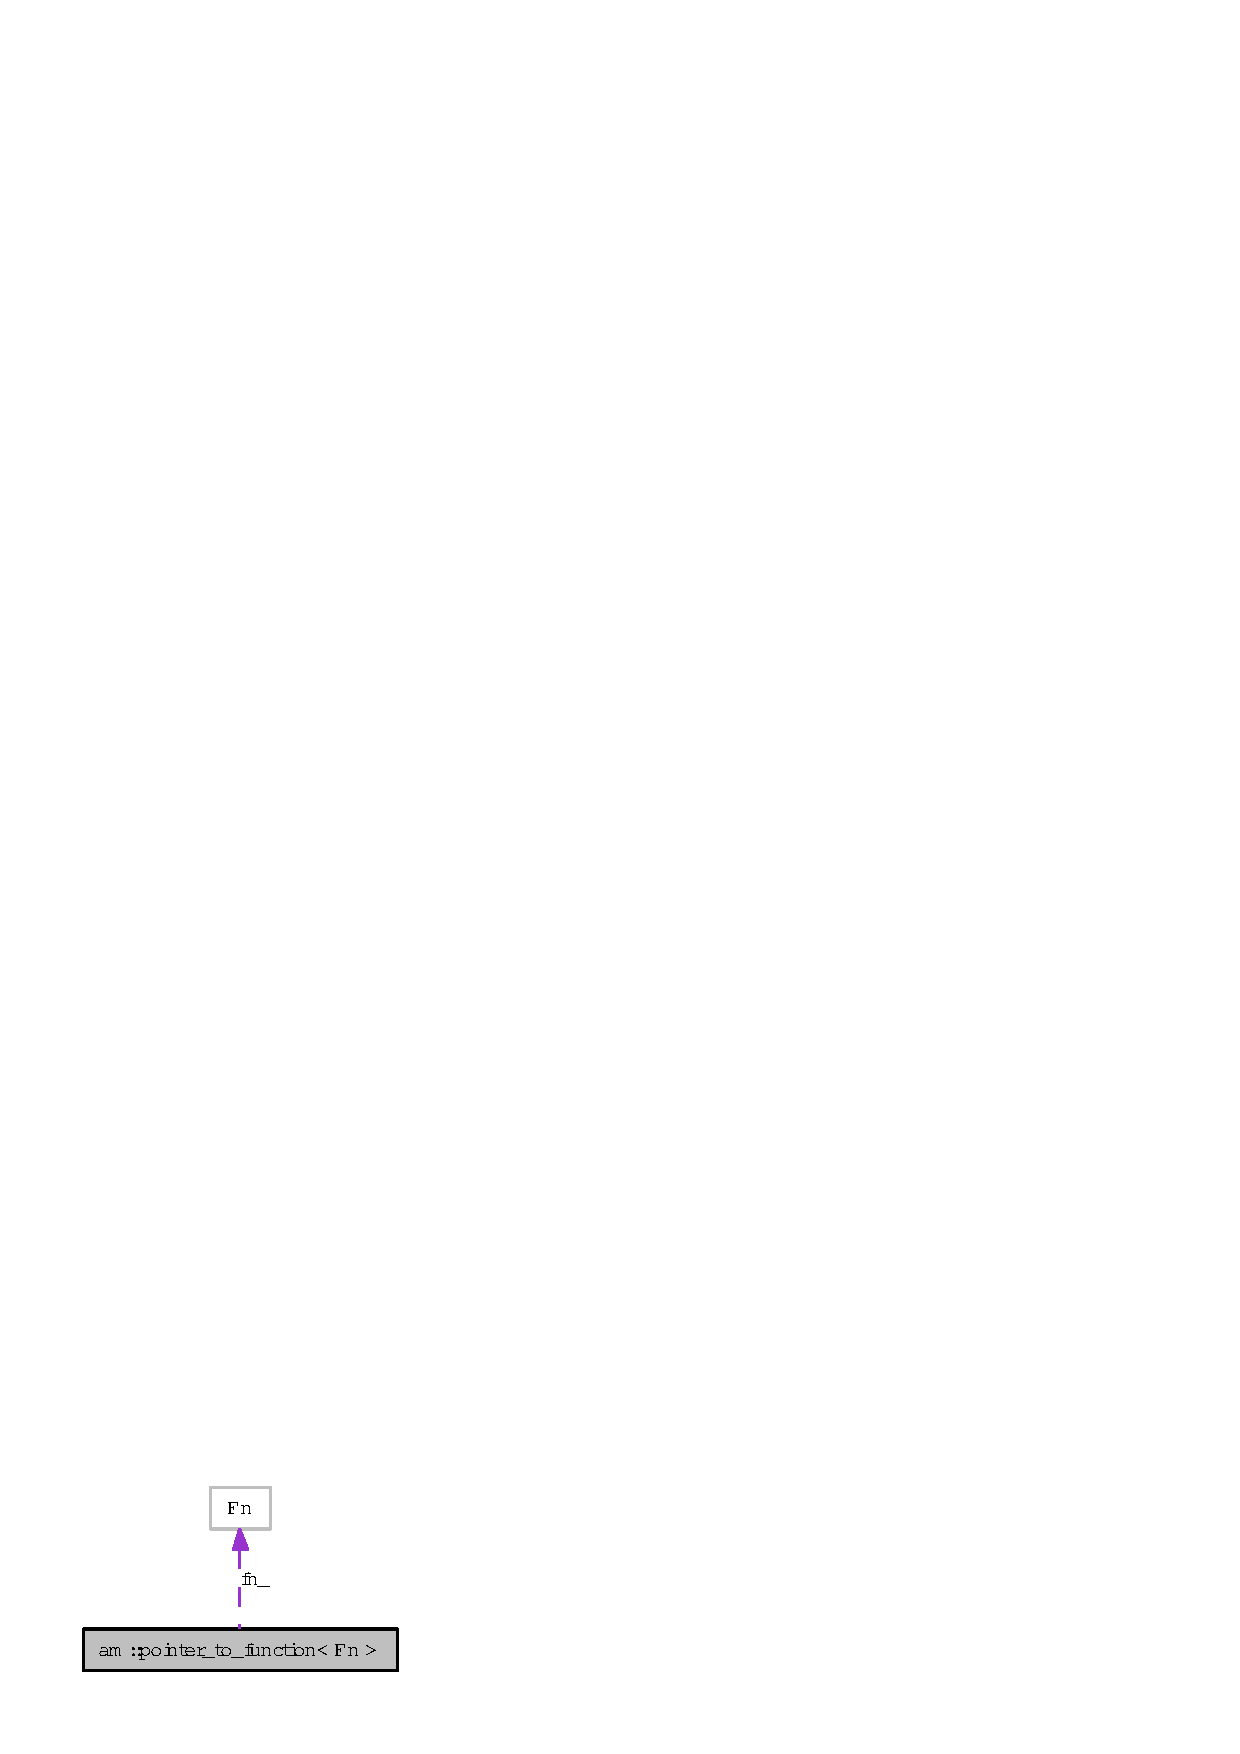
\includegraphics[width=97pt]{structam_1_1pointer__to__function__coll__graph}
\end{center}
\end{figure}
\subsection*{Public Types}
\begin{CompactItemize}
\item 
typedef void \textbf{result\_\-type}\label{structam_1_1pointer__to__function_818851d1f56e4c2442dd06fe8e2d3e7d}

\end{CompactItemize}
\subsection*{Public Member Functions}
\begin{CompactItemize}
\item 
\textbf{pointer\_\-to\_\-function} (Fn const fn)\label{structam_1_1pointer__to__function_8ab9fefd6c4889000e9d19639c9cc523}

\item 
template$<$typename P1$>$ void \textbf{operator()} (P1 p1) const \label{structam_1_1pointer__to__function_9cc0e0580a8bdc665fce79a4512c72e4}

\item 
template$<$typename P1, typename P2$>$ void \textbf{operator()} (P1 p1, P2 p2) const\label{structam_1_1pointer__to__function_94ee89fd2eece28225290212b5feadf1}

\end{CompactItemize}
\subsection*{Public Attributes}
\begin{CompactItemize}
\item 
Fn const \textbf{fn\_\-}\label{structam_1_1pointer__to__function_1445b4cac44889d1cdbab008dc773c6d}

\end{CompactItemize}


\subsection{Detailed Description}
\subsubsection*{template$<$typename Fn$>$ struct am::pointer\_\-to\_\-function$<$ Fn $>$}

Function pointer to an unary function or a binary function. 

It is not a std::unary\_\-function nor a std::binary\_\-function, but works for any calling convention.

\begin{Desc}
\item[See also:]\doxyref{ptr\_\-fun()}{p.}{namespaceam_075d855cc1ab6d87a818e72ed34bc829} \end{Desc}




The documentation for this struct was generated from the following file:\begin{CompactItemize}
\item 
{\bf mate.hpp}\end{CompactItemize}

\section{am::ref\_\-holder$<$ T $>$ Class Template Reference}
\label{classam_1_1ref__holder}\index{am::ref_holder@{am::ref\_\-holder}}
Reference holder.  


{\tt \#include $<$mate.hpp$>$}

Collaboration diagram for am::ref\_\-holder$<$ T $>$:\begin{figure}[H]
\begin{center}
\leavevmode
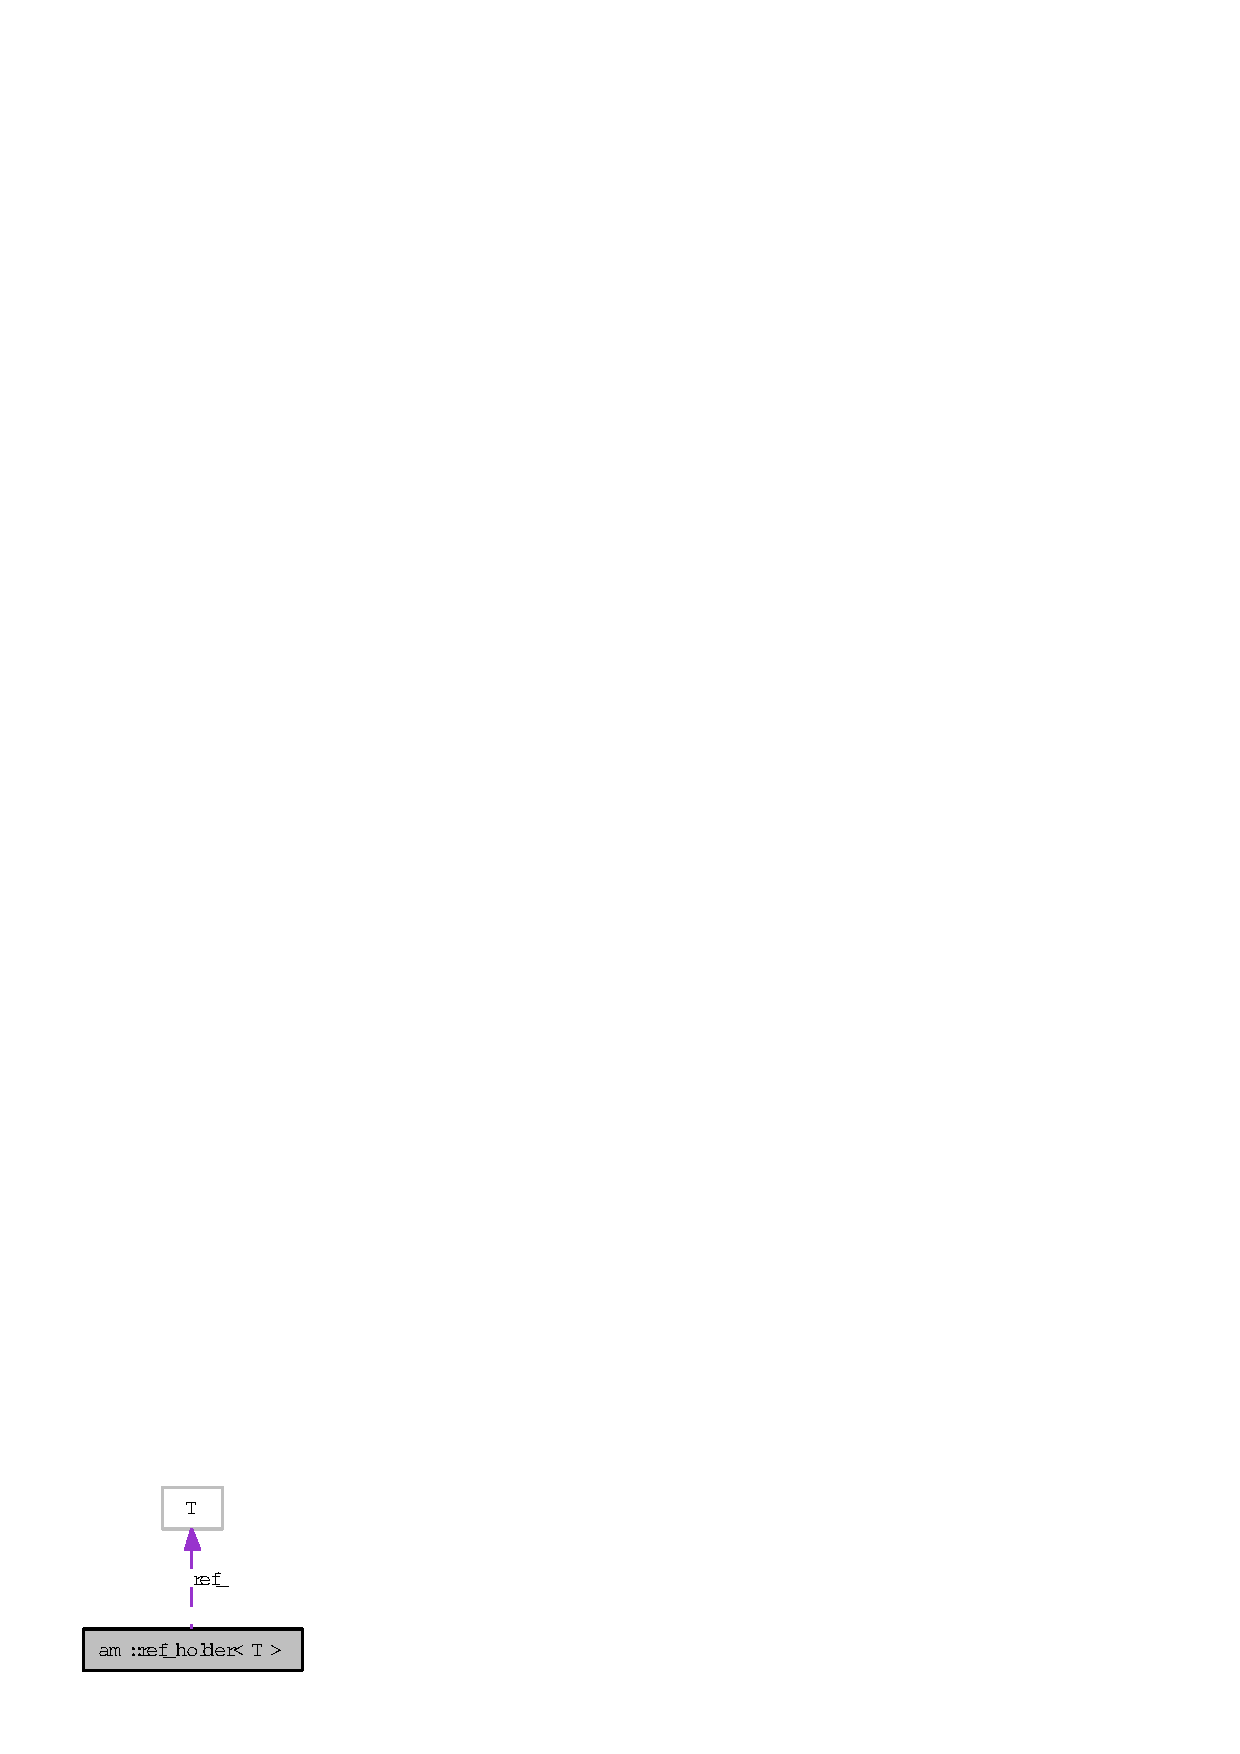
\includegraphics[width=74pt]{classam_1_1ref__holder__coll__graph}
\end{center}
\end{figure}
\subsection*{Public Member Functions}
\begin{CompactItemize}
\item 
\textbf{ref\_\-holder} (T \&ref)\label{classam_1_1ref__holder_69c06480a81cc5adf93a44c074f7d8b9}

\item 
\textbf{ref\_\-holder} ({\bf ref\_\-holder}$<$ T $>$ const \&other)\label{classam_1_1ref__holder_b88950b0f62bda1bd88b0debec990886}

\item 
{\bf ref\_\-holder}$<$ T $>$ \& \textbf{operator=} ({\bf ref\_\-holder}$<$ T $>$ const \&other)\label{classam_1_1ref__holder_94350a442e4692a9715e8d57cf765443}

\item 
\textbf{operator T \&} () const\label{classam_1_1ref__holder_75b03d6e929a13109da0635182da9b56}

\end{CompactItemize}
\subsection*{Private Attributes}
\begin{CompactItemize}
\item 
T \& \textbf{ref\_\-}\label{classam_1_1ref__holder_5fcb17879a5ec684f7c68912b6e8120b}

\end{CompactItemize}


\subsection{Detailed Description}
\subsubsection*{template$<$class T$>$ class am::ref\_\-holder$<$ T $>$}

Reference holder. 

Supports parameters by reference. It is used to \char`\"{}feed\char`\"{} reference to mate function since the input argument of the mate function is only passed by value. This class transforms a reference into a value.

\begin{Desc}
\item[See also:]\doxyref{ref()}{p.}{namespaceam_aeac214784a5e1a16be743677555cb96}, \doxyref{cref()}{p.}{namespaceam_10096add639d0ba375c58c53aa8ff4a7} \end{Desc}




The documentation for this class was generated from the following file:\begin{CompactItemize}
\item 
{\bf mate.hpp}\end{CompactItemize}

\section{am::detail::simple\_\-ptr\_\-holder Class Reference}
\label{classam_1_1detail_1_1simple__ptr__holder}\index{am::detail::simple_ptr_holder@{am::detail::simple\_\-ptr\_\-holder}}
{\tt \#include $<$mate.hpp$>$}

\subsection*{Public Member Functions}
\begin{CompactItemize}
\item 
template$<$class T$>$ \textbf{simple\_\-ptr\_\-holder} (T $\ast$ptr)\label{classam_1_1detail_1_1simple__ptr__holder_2f1481e35d91fe069c2e4b5ce1e62190}

\item 
\textbf{simple\_\-ptr\_\-holder} ({\bf simple\_\-ptr\_\-holder} const \&other)\label{classam_1_1detail_1_1simple__ptr__holder_42d5461ff01a8b5def157e79af43947d}

\item 
void $\ast$ \textbf{get} () const\label{classam_1_1detail_1_1simple__ptr__holder_7d87eeccfa11890cf7ffac424972205a}

\item 
bool \textbf{empty} () const\label{classam_1_1detail_1_1simple__ptr__holder_7cee3cc13012dc1b5d8f3c302533b3c5}

\item 
void \textbf{reset} ()\label{classam_1_1detail_1_1simple__ptr__holder_b8fd1365e058fba7c0270cc08d2f2599}

\end{CompactItemize}
\subsection*{Private Types}
\begin{CompactItemize}
\item 
typedef void($\ast$) \textbf{typeless\_\-deleter\_\-stub} (void $\ast$)\label{classam_1_1detail_1_1simple__ptr__holder_e0a1a8bbf6d7a1b4897df97eb3b5523f}

\end{CompactItemize}
\subsection*{Private Member Functions}
\begin{CompactItemize}
\item 
{\bf simple\_\-ptr\_\-holder} \& \textbf{operator=} ({\bf simple\_\-ptr\_\-holder} const \&)\label{classam_1_1detail_1_1simple__ptr__holder_b8a07a0e314e931f893ad3137a8cccbb}

\end{CompactItemize}
\subsection*{Private Attributes}
\begin{CompactItemize}
\item 
void $\ast$ \textbf{ptr\_\-}\label{classam_1_1detail_1_1simple__ptr__holder_a917d43dc53ccd659ad5e452a06faad3}

\item 
typeless\_\-deleter\_\-stub \textbf{deleter\_\-stub\_\-}\label{classam_1_1detail_1_1simple__ptr__holder_9921d838af2d228eb1b635d6697d1569}

\end{CompactItemize}
\subsection*{Classes}
\begin{CompactItemize}
\item 
struct \textbf{typed\_\-}
\end{CompactItemize}


\subsection{Detailed Description}
\begin{Desc}
\item[For internal use only.]
Simple pointer holder. Store a pointer and delete it in type safe manner in its destructor when it goes out of scope. \end{Desc}




The documentation for this class was generated from the following file:\begin{CompactItemize}
\item 
{\bf mate.hpp}\end{CompactItemize}

\section{am::lambda::detail::tr$<$ V $>$ Struct Template Reference}
\label{structam_1_1lambda_1_1detail_1_1tr}\index{am::lambda::detail::tr@{am::lambda::detail::tr}}
{\tt \#include $<$lambda.hpp$>$}

\subsection*{Public Types}
\begin{CompactItemize}
\item 
typedef {\bf if\_\-}$<$ {\bf is\_\-lambda\_\-op}$<$ V $>$::value, V, {\bf lambda\_\-val}$<$ V $>$ $>$::type \textbf{type}\label{structam_1_1lambda_1_1detail_1_1tr_acd6ff734f1b3f1c9fdb24f75c34ccf5}

\end{CompactItemize}


\subsection{Detailed Description}
\subsubsection*{template$<$class V$>$ struct am::lambda::detail::tr$<$ V $>$}

\begin{Desc}
\item[For internal use only.]
Transform a value to a lambda value \end{Desc}




The documentation for this struct was generated from the following file:\begin{CompactItemize}
\item 
{\bf lambda.hpp}\end{CompactItemize}

\section{am::lambda::detail::tr$<$ var\_\-type1 $>$ Struct Template Reference}
\label{structam_1_1lambda_1_1detail_1_1tr_3_01var__type1_01_4}\index{am::lambda::detail::tr< var_type1 >@{am::lambda::detail::tr$<$ var\_\-type1 $>$}}
{\tt \#include $<$lambda.hpp$>$}

\subsection*{Public Types}
\begin{CompactItemize}
\item 
typedef {\bf var\_\-type1} \textbf{type}\label{structam_1_1lambda_1_1detail_1_1tr_3_01var__type1_01_4_2f07af356e0bb0d9d1b18d781b1a2b48}

\end{CompactItemize}


\subsection{Detailed Description}
\subsubsection*{template$<$$>$ struct am::lambda::detail::tr$<$ var\_\-type1 $>$}

\begin{Desc}
\item[For internal use only.]
Template specialization for the 1st lambda place holder. \end{Desc}




The documentation for this struct was generated from the following file:\begin{CompactItemize}
\item 
{\bf lambda.hpp}\end{CompactItemize}

\section{am::lambda::detail::tr$<$ var\_\-type2 $>$ Struct Template Reference}
\label{structam_1_1lambda_1_1detail_1_1tr_3_01var__type2_01_4}\index{am::lambda::detail::tr< var_type2 >@{am::lambda::detail::tr$<$ var\_\-type2 $>$}}
{\tt \#include $<$lambda.hpp$>$}

\subsection*{Public Types}
\begin{CompactItemize}
\item 
typedef {\bf var\_\-type2} \textbf{type}\label{structam_1_1lambda_1_1detail_1_1tr_3_01var__type2_01_4_c7796eb0140b1f516c2cae9fec615815}

\end{CompactItemize}


\subsection{Detailed Description}
\subsubsection*{template$<$$>$ struct am::lambda::detail::tr$<$ var\_\-type2 $>$}

\begin{Desc}
\item[For internal use only.]
Template specialization for the 2nd lambda place holder. \end{Desc}




The documentation for this struct was generated from the following file:\begin{CompactItemize}
\item 
{\bf lambda.hpp}\end{CompactItemize}

\section{am::lambda::detail::tr$<$ var\_\-type3 $>$ Struct Template Reference}
\label{structam_1_1lambda_1_1detail_1_1tr_3_01var__type3_01_4}\index{am::lambda::detail::tr< var_type3 >@{am::lambda::detail::tr$<$ var\_\-type3 $>$}}
{\tt \#include $<$lambda.hpp$>$}

\subsection*{Public Types}
\begin{CompactItemize}
\item 
typedef {\bf var\_\-type3} \textbf{type}\label{structam_1_1lambda_1_1detail_1_1tr_3_01var__type3_01_4_f69f2d9151de08941730cd0252ba93eb}

\end{CompactItemize}


\subsection{Detailed Description}
\subsubsection*{template$<$$>$ struct am::lambda::detail::tr$<$ var\_\-type3 $>$}

\begin{Desc}
\item[For internal use only.]
Template specialization for the 3rd lambda place holder. \end{Desc}




The documentation for this struct was generated from the following file:\begin{CompactItemize}
\item 
{\bf lambda.hpp}\end{CompactItemize}

\section{am::lambda::var\_\-type1 Struct Reference}
\label{structam_1_1lambda_1_1var__type1}\index{am::lambda::var_type1@{am::lambda::var\_\-type1}}
{\tt \#include $<$lambda.hpp$>$}

\subsection*{Public Member Functions}
\begin{CompactItemize}
\item 
{\bf address\_\-of} \textbf{operator \&} () const\label{structam_1_1lambda_1_1var__type1_f8eaa82c77daba44d3aed685a3304b10}

\item 
template$<$class T1, class T2, class T3$>$ T1 \& \textbf{operator()} (T1 \&t1, T2, T3) const \label{structam_1_1lambda_1_1var__type1_0bd48ce6c2c88fa3b0025f50f8d7ea60}

\item 
template$<$class T1, class T2$>$ T1 \& \textbf{operator()} (T1 \&t1, T2) const\label{structam_1_1lambda_1_1var__type1_740a4d3e513892cf02fb251aabd98923}

\item 
template$<$class T1$>$ T1 \& \textbf{operator()} (T1 \&t1) const\label{structam_1_1lambda_1_1var__type1_e408c4a011310bb264ce39aa2832501b}

\end{CompactItemize}
\subsection*{Private Member Functions}
\begin{CompactItemize}
\item 
void \textbf{operator()} () const\label{structam_1_1lambda_1_1var__type1_91b07bba79271aade1600d8970932b39}

\end{CompactItemize}
\subsection*{Classes}
\begin{CompactItemize}
\item 
struct {\bf address\_\-of}
\end{CompactItemize}


\subsection{Detailed Description}
\begin{Desc}
\item[For internal use only.]
1st lambda place holder type. \end{Desc}




The documentation for this struct was generated from the following file:\begin{CompactItemize}
\item 
{\bf lambda.hpp}\end{CompactItemize}

\section{am::lambda::var\_\-type1::address\_\-of Struct Reference}
\label{structam_1_1lambda_1_1var__type1_1_1address__of}\index{am::lambda::var_type1::address_of@{am::lambda::var\_\-type1::address\_\-of}}
{\tt \#include $<$lambda.hpp$>$}

Inherits {\bf am::lambda::detail::lambda\_\-op\_\-tag}.

Inheritance diagram for am::lambda::var\_\-type1::address\_\-of:\begin{figure}[H]
\begin{center}
\leavevmode
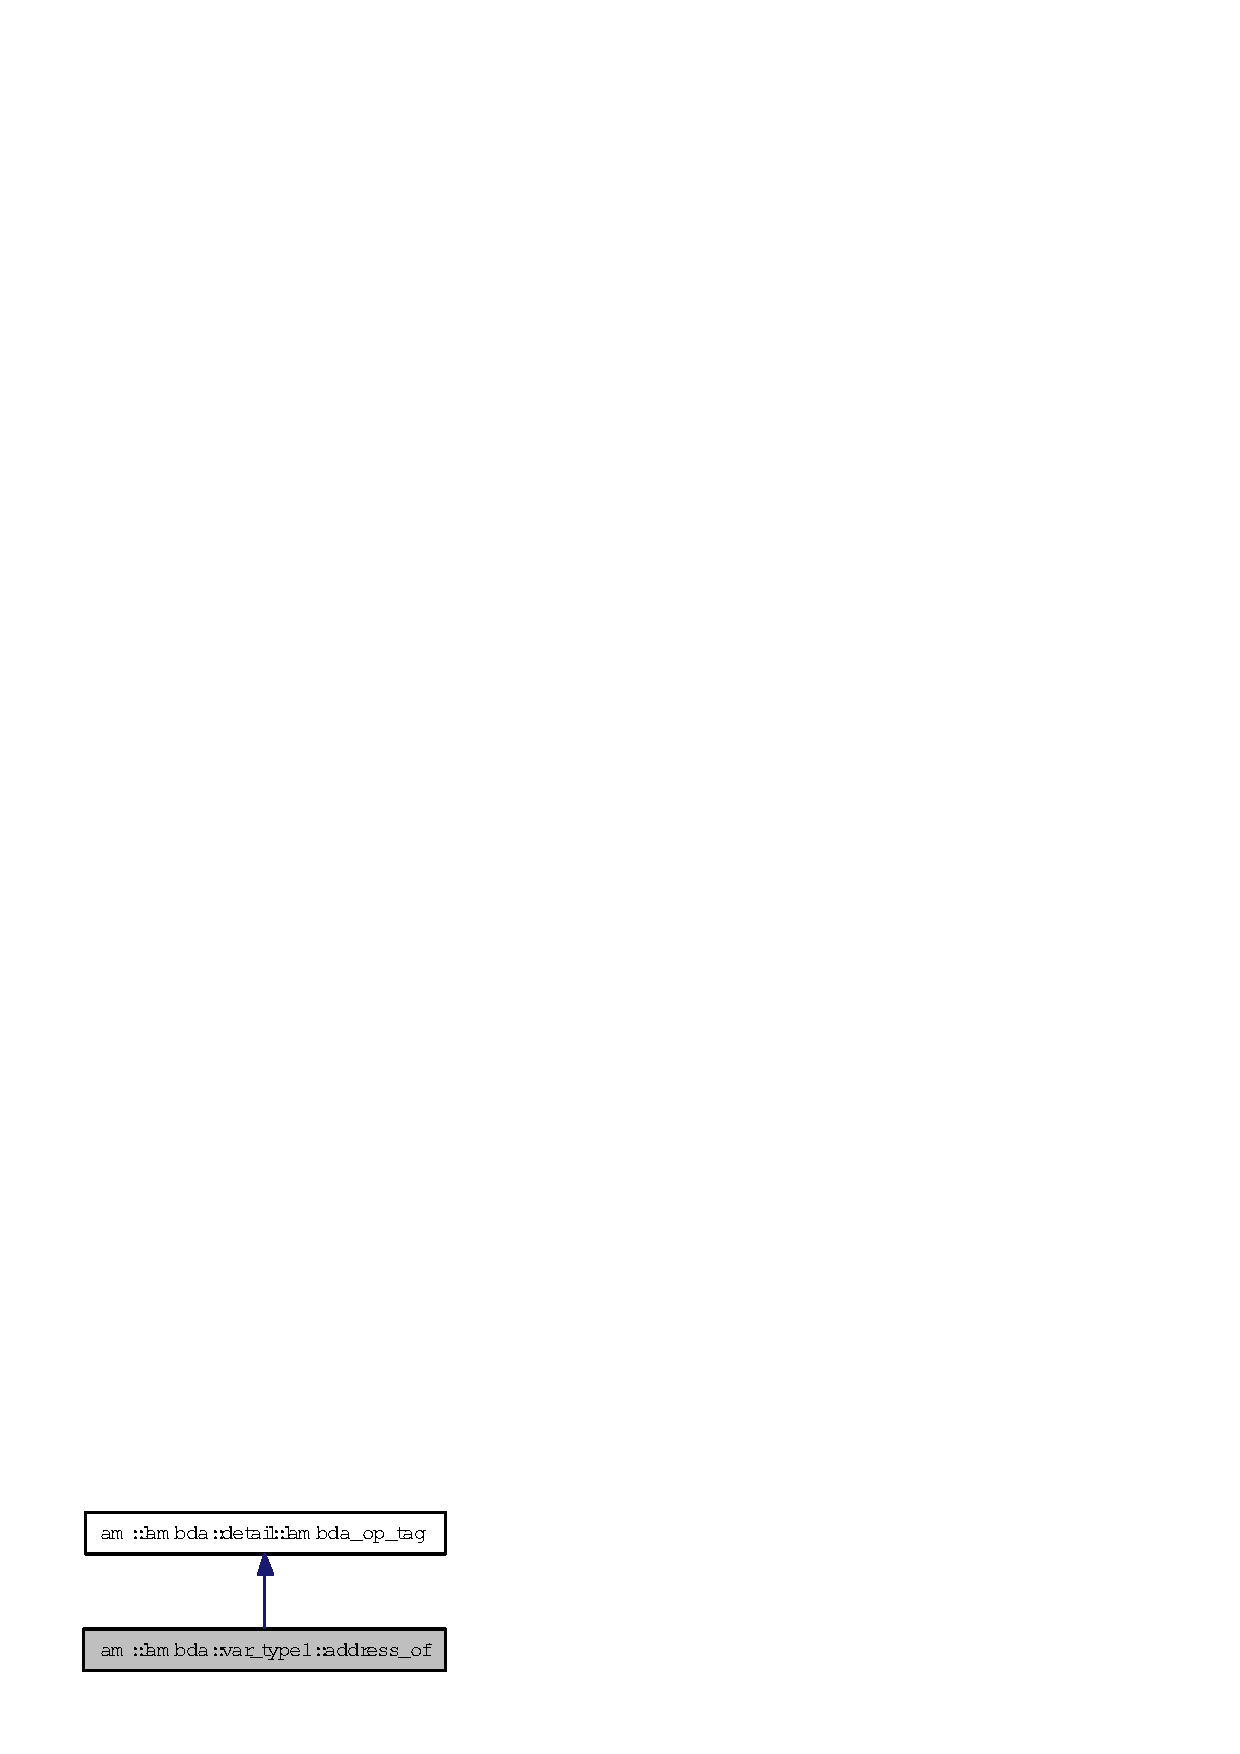
\includegraphics[width=109pt]{structam_1_1lambda_1_1var__type1_1_1address__of__inherit__graph}
\end{center}
\end{figure}
Collaboration diagram for am::lambda::var\_\-type1::address\_\-of:\begin{figure}[H]
\begin{center}
\leavevmode
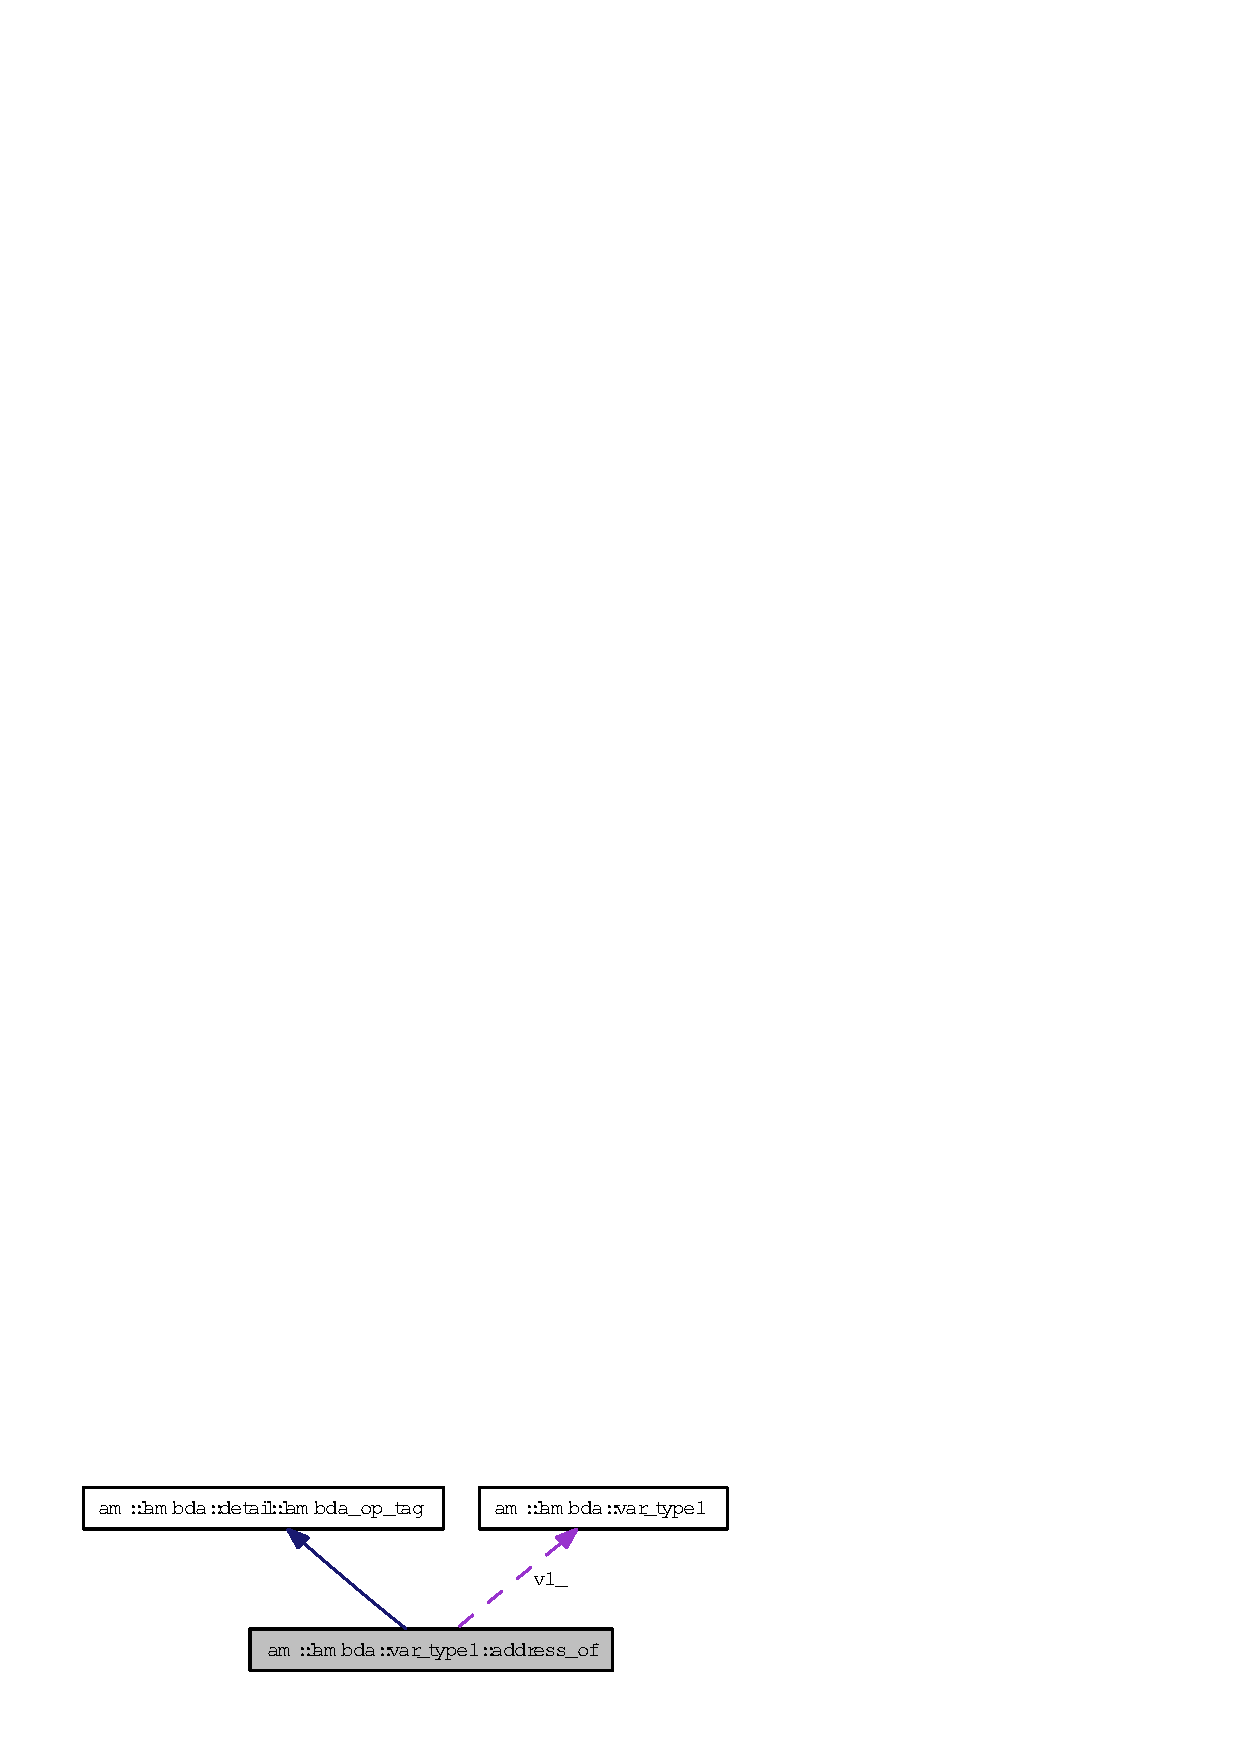
\includegraphics[width=176pt]{structam_1_1lambda_1_1var__type1_1_1address__of__coll__graph}
\end{center}
\end{figure}
\subsection*{Public Member Functions}
\begin{CompactItemize}
\item 
\textbf{address\_\-of} ({\bf var\_\-type1} const \&v1)\label{structam_1_1lambda_1_1var__type1_1_1address__of_72b07ff04f5f08b8a7d11fc84b48c099}

\item 
template$<$class T1, class T2, class T3$>$ T1 $\ast$ \textbf{operator()} (T1 \&t1, T2 \&t2, T3 \&t3) const \label{structam_1_1lambda_1_1var__type1_1_1address__of_eee7a6c91e1d5cd7d7b4816385388373}

\item 
template$<$class T1, class T2$>$ T1 $\ast$ \textbf{operator()} (T1 \&t1, T2 \&t2) const \label{structam_1_1lambda_1_1var__type1_1_1address__of_eb8776973b8225d88f2694017370689b}

\item 
template$<$class T1$>$ T1 $\ast$ \textbf{operator()} (T1 \&t1) const\label{structam_1_1lambda_1_1var__type1_1_1address__of_c51b44f1018decf79f174c1eaa9cff8d}

\end{CompactItemize}
\subsection*{Public Attributes}
\begin{CompactItemize}
\item 
{\bf var\_\-type1} const \& \textbf{v1\_\-}\label{structam_1_1lambda_1_1var__type1_1_1address__of_f114d1c8dd1b4ad46f76b7af87d1c995}

\end{CompactItemize}


\subsection{Detailed Description}
\begin{Desc}
\item[For internal use only.]
\doxyref{address\_\-of}{p.}{structam_1_1lambda_1_1var__type1_1_1address__of} pure function. Return the address of the variable type 1.

\begin{Desc}
\item[See also:]operator \&() \end{Desc}
\end{Desc}




The documentation for this struct was generated from the following file:\begin{CompactItemize}
\item 
{\bf lambda.hpp}\end{CompactItemize}

\section{am::lambda::var\_\-type2 Struct Reference}
\label{structam_1_1lambda_1_1var__type2}\index{am::lambda::var_type2@{am::lambda::var\_\-type2}}
{\tt \#include $<$lambda.hpp$>$}

\subsection*{Public Member Functions}
\begin{CompactItemize}
\item 
{\bf address\_\-of} \textbf{operator \&} () const\label{structam_1_1lambda_1_1var__type2_e7fd2044c8ff27cca60e67190c7f9f85}

\item 
template$<$class T1, class T2, class T3$>$ T2 \& \textbf{operator()} (T1, T2 \&t2, T3) const \label{structam_1_1lambda_1_1var__type2_35e555861fad0cfd5175395351d919b1}

\item 
template$<$class T1, class T2$>$ T2 \& \textbf{operator()} (T1, T2 \&t2) const\label{structam_1_1lambda_1_1var__type2_bf4ee948158be0c7d229d1769c488f1b}

\end{CompactItemize}
\subsection*{Private Member Functions}
\begin{CompactItemize}
\item 
template$<$class T1$>$ T1 \textbf{operator()} (T1) const\label{structam_1_1lambda_1_1var__type2_b2a146d22913d79e8fa2642ff3920e28}

\item 
void \textbf{operator()} () const\label{structam_1_1lambda_1_1var__type2_d91f2a4f7c04d193a26355f8e20f83c1}

\end{CompactItemize}
\subsection*{Classes}
\begin{CompactItemize}
\item 
struct {\bf address\_\-of}
\end{CompactItemize}


\subsection{Detailed Description}
\begin{Desc}
\item[For internal use only.]
2nd lambda place holder type. \end{Desc}




The documentation for this struct was generated from the following file:\begin{CompactItemize}
\item 
{\bf lambda.hpp}\end{CompactItemize}

\section{am::lambda::var\_\-type2::address\_\-of Struct Reference}
\label{structam_1_1lambda_1_1var__type2_1_1address__of}\index{am::lambda::var_type2::address_of@{am::lambda::var\_\-type2::address\_\-of}}
{\tt \#include $<$lambda.hpp$>$}

Inherits {\bf am::lambda::detail::lambda\_\-op\_\-tag}.

Inheritance diagram for am::lambda::var\_\-type2::address\_\-of:\begin{figure}[H]
\begin{center}
\leavevmode
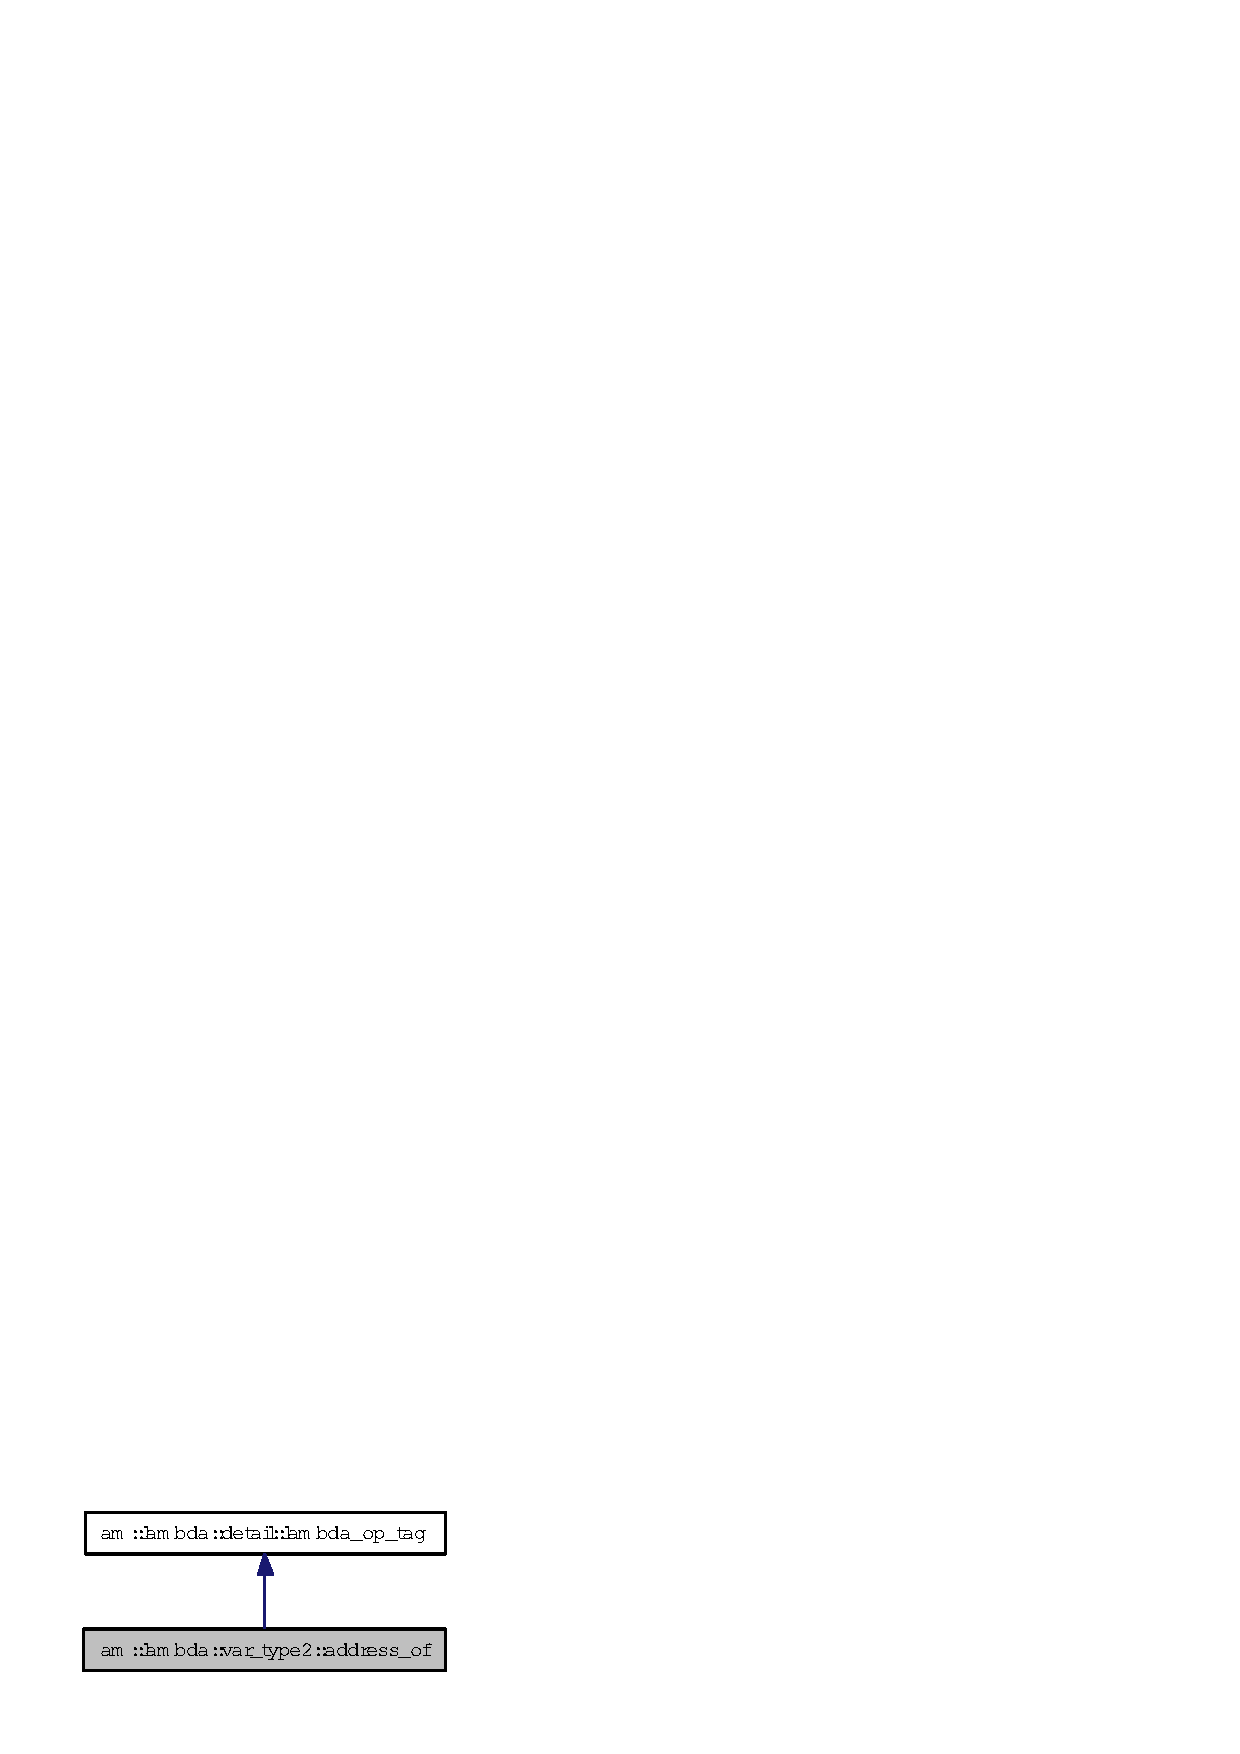
\includegraphics[width=109pt]{structam_1_1lambda_1_1var__type2_1_1address__of__inherit__graph}
\end{center}
\end{figure}
Collaboration diagram for am::lambda::var\_\-type2::address\_\-of:\begin{figure}[H]
\begin{center}
\leavevmode
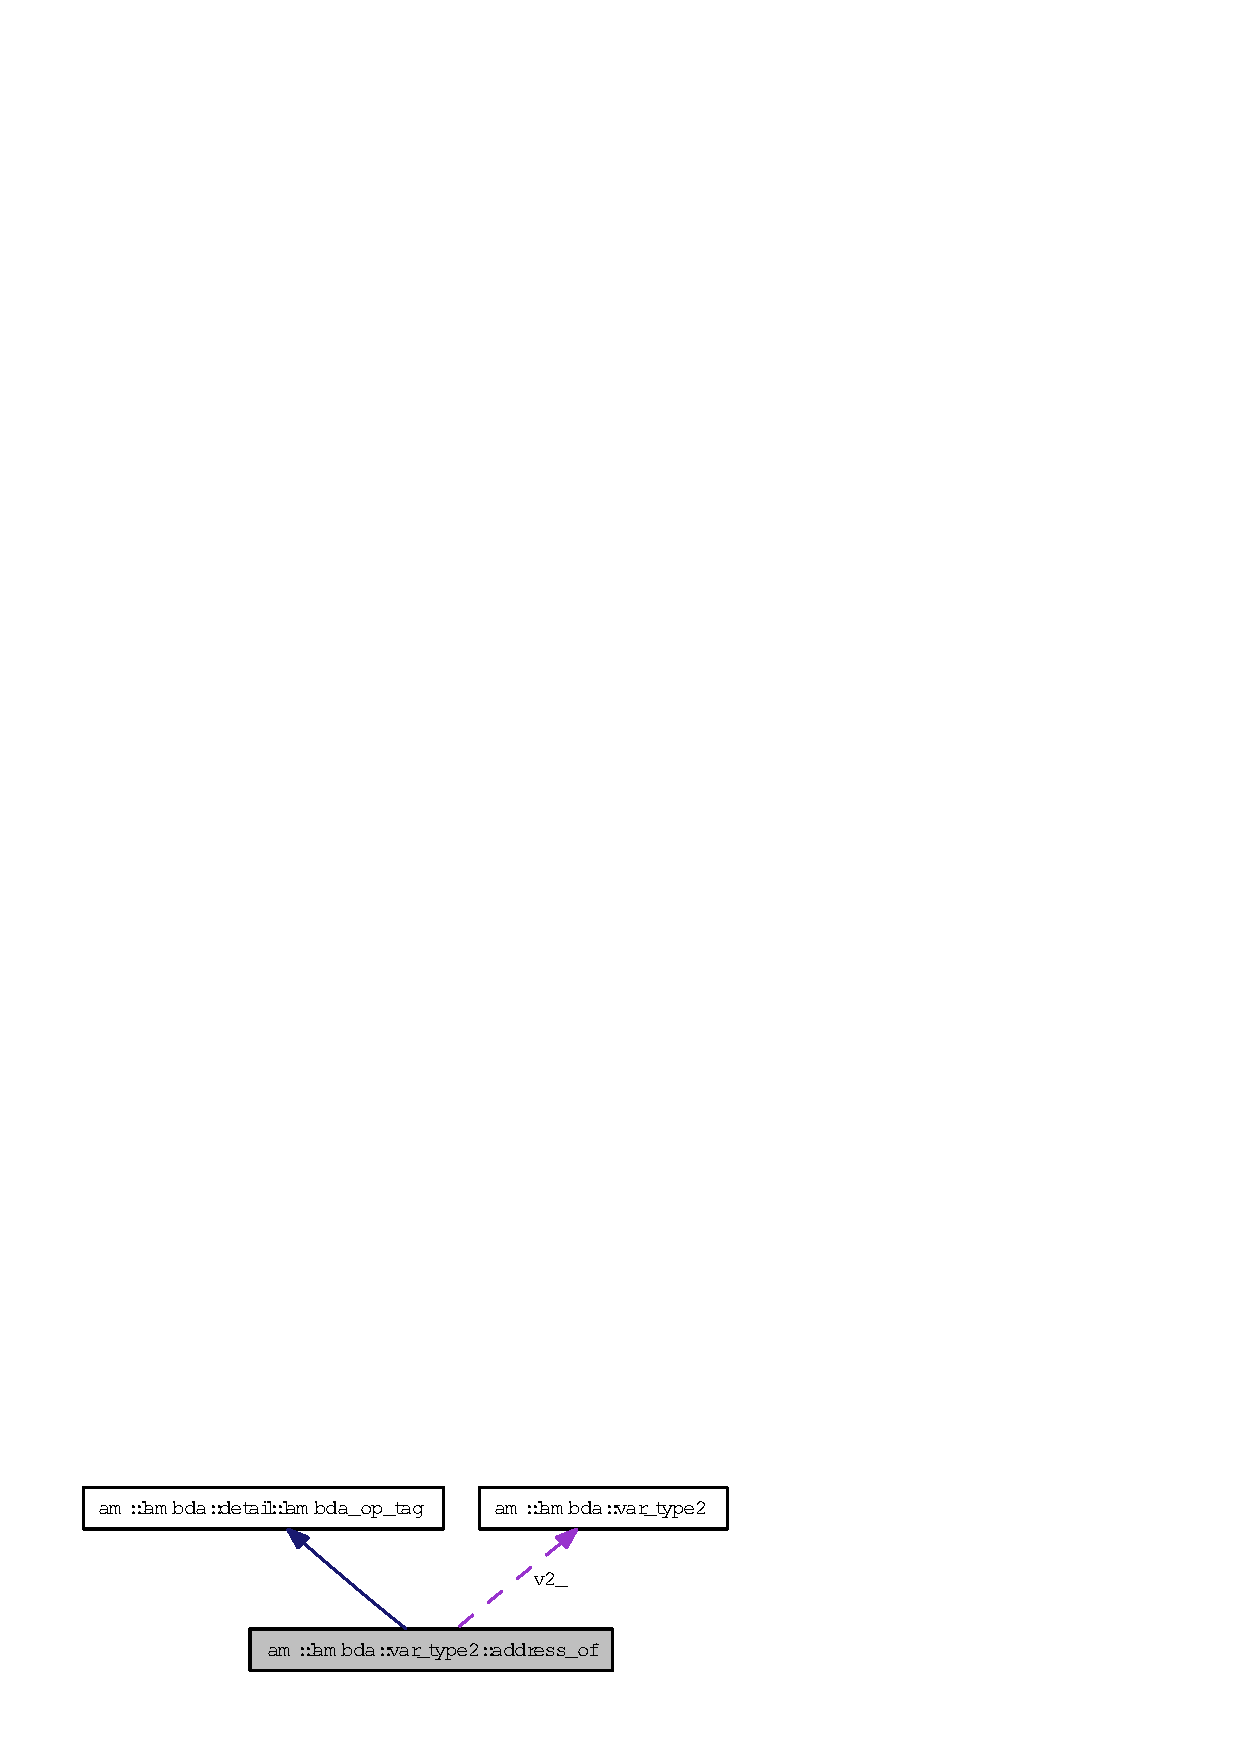
\includegraphics[width=176pt]{structam_1_1lambda_1_1var__type2_1_1address__of__coll__graph}
\end{center}
\end{figure}
\subsection*{Public Member Functions}
\begin{CompactItemize}
\item 
\textbf{address\_\-of} ({\bf var\_\-type2} const \&v2)\label{structam_1_1lambda_1_1var__type2_1_1address__of_1a07042e900fca785a9dff2436e0f165}

\item 
template$<$class T1, class T2, class T3$>$ T2 $\ast$ \textbf{operator()} (T1 \&t1, T2 \&t2, T3 \&t3) const \label{structam_1_1lambda_1_1var__type2_1_1address__of_ba6325b1f85eefc0b78f0fc755d6f09b}

\item 
template$<$class T1, class T2$>$ T2 $\ast$ \textbf{operator()} (T1 \&t1, T2 \&t2) const \label{structam_1_1lambda_1_1var__type2_1_1address__of_37ee13dc0b3f453aa7292c62a7a59e67}

\end{CompactItemize}
\subsection*{Public Attributes}
\begin{CompactItemize}
\item 
{\bf var\_\-type2} const \& \textbf{v2\_\-}\label{structam_1_1lambda_1_1var__type2_1_1address__of_9531dcc998c7866c271d1f96744a5ca1}

\end{CompactItemize}


\subsection{Detailed Description}
\begin{Desc}
\item[For internal use only.]
\doxyref{address\_\-of}{p.}{structam_1_1lambda_1_1var__type2_1_1address__of} pure function. Return the address of the variable type 1.

\begin{Desc}
\item[See also:]operator \&() \end{Desc}
\end{Desc}




The documentation for this struct was generated from the following file:\begin{CompactItemize}
\item 
{\bf lambda.hpp}\end{CompactItemize}

\section{am::lambda::var\_\-type3 Struct Reference}
\label{structam_1_1lambda_1_1var__type3}\index{am::lambda::var_type3@{am::lambda::var\_\-type3}}
{\tt \#include $<$lambda.hpp$>$}

\subsection*{Public Member Functions}
\begin{CompactItemize}
\item 
{\bf address\_\-of} \textbf{operator \&} () const\label{structam_1_1lambda_1_1var__type3_d70273bbdc95b750251428c0eb831fdb}

\item 
template$<$class T1, class T2, class T3$>$ T3 \& \textbf{operator()} (T1, T2, T3 \&t3) const \label{structam_1_1lambda_1_1var__type3_a8a9aedd1d2d3714d320cb50cfb27513}

\end{CompactItemize}
\subsection*{Private Member Functions}
\begin{CompactItemize}
\item 
template$<$class T1, class T2$>$ T2 \textbf{operator()} (T1, T2) const\label{structam_1_1lambda_1_1var__type3_56ec18403573441e1d51230f0ac3e329}

\item 
template$<$class T1$>$ T1 \textbf{operator()} (T1) const\label{structam_1_1lambda_1_1var__type3_3f0fe23b87a27e08975e8008d4770238}

\item 
void \textbf{operator()} () const\label{structam_1_1lambda_1_1var__type3_2ab55cffd256fd61668651febe6f9f37}

\end{CompactItemize}
\subsection*{Classes}
\begin{CompactItemize}
\item 
struct {\bf address\_\-of}
\end{CompactItemize}


\subsection{Detailed Description}
\begin{Desc}
\item[For internal use only.]
3rd lambda place holder type. \end{Desc}




The documentation for this struct was generated from the following file:\begin{CompactItemize}
\item 
{\bf lambda.hpp}\end{CompactItemize}

\section{am::lambda::var\_\-type3::address\_\-of Struct Reference}
\label{structam_1_1lambda_1_1var__type3_1_1address__of}\index{am::lambda::var_type3::address_of@{am::lambda::var\_\-type3::address\_\-of}}
{\tt \#include $<$lambda.hpp$>$}

Inherits {\bf am::lambda::detail::lambda\_\-op\_\-tag}.

Inheritance diagram for am::lambda::var\_\-type3::address\_\-of:\begin{figure}[H]
\begin{center}
\leavevmode
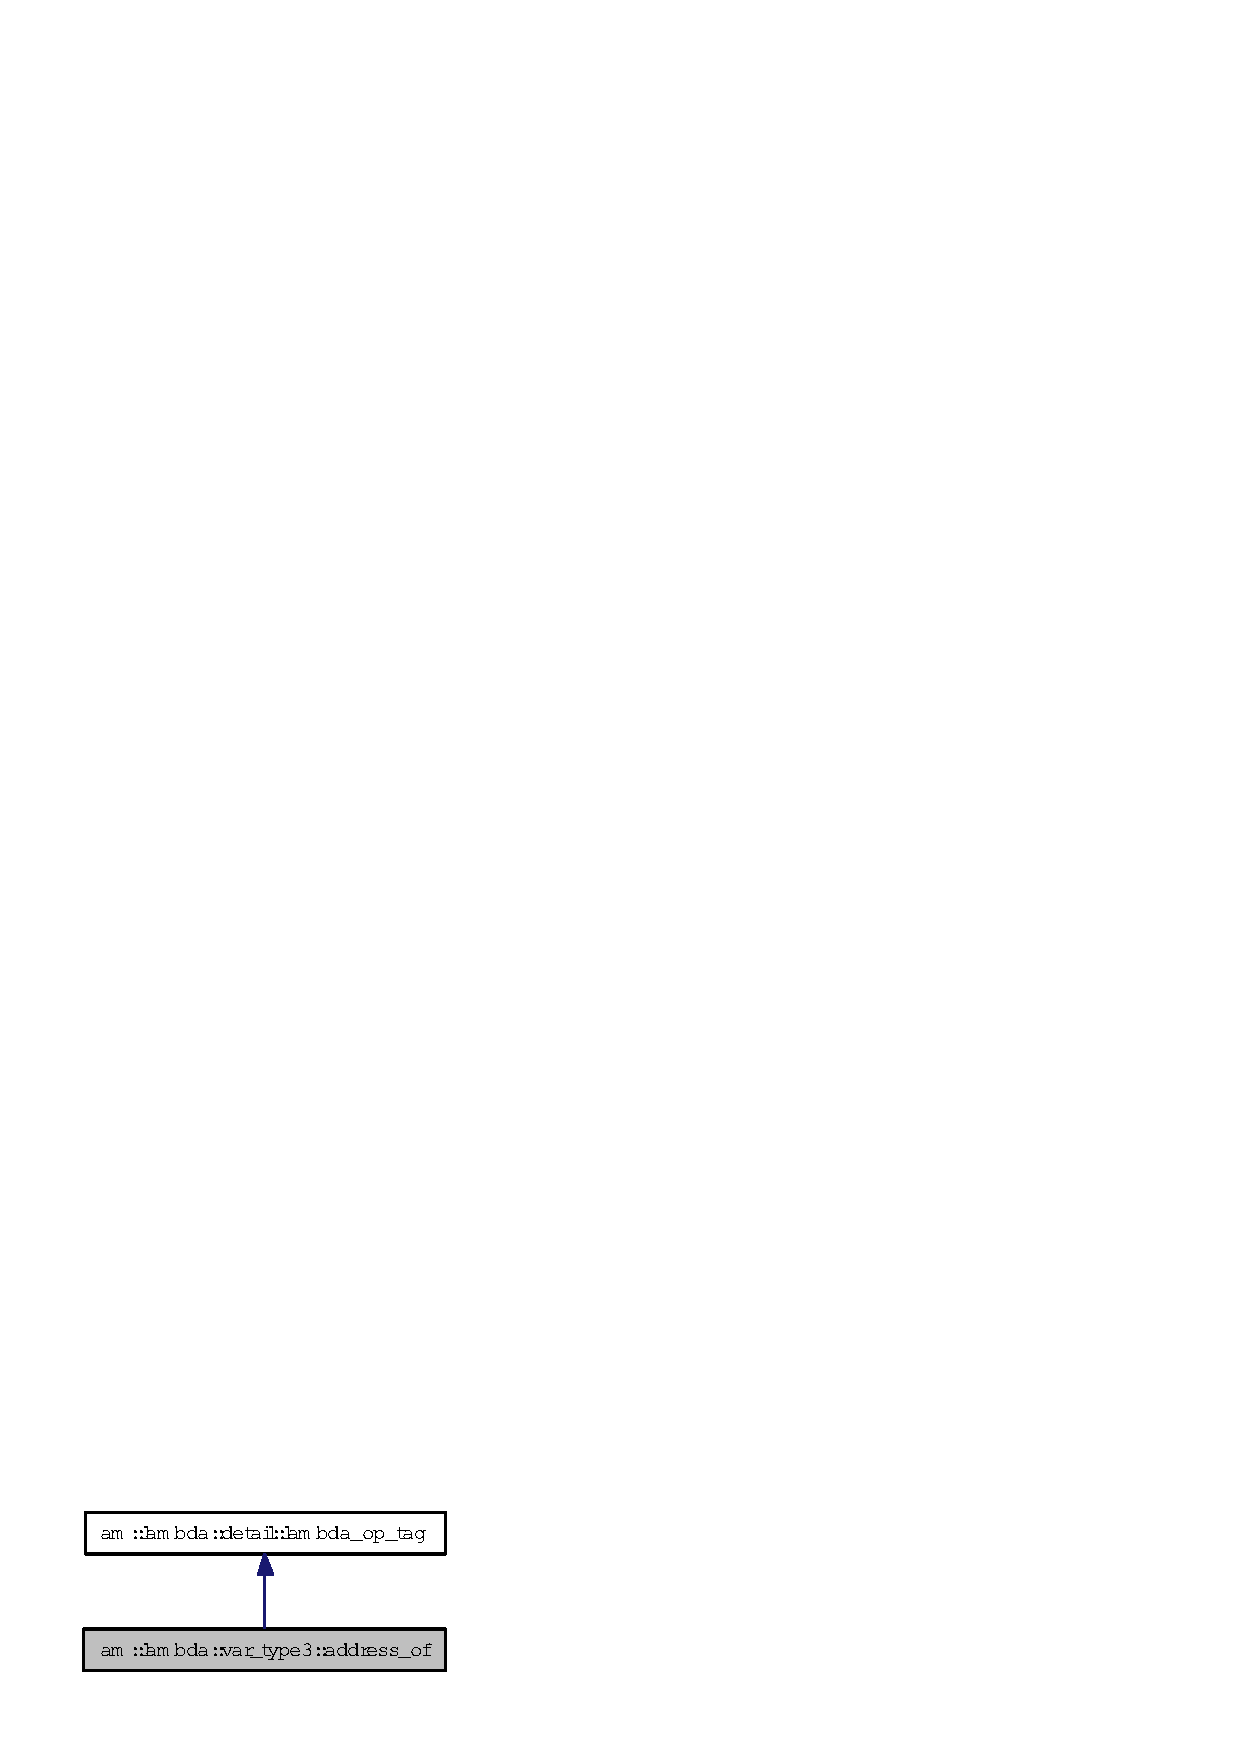
\includegraphics[width=109pt]{structam_1_1lambda_1_1var__type3_1_1address__of__inherit__graph}
\end{center}
\end{figure}
Collaboration diagram for am::lambda::var\_\-type3::address\_\-of:\begin{figure}[H]
\begin{center}
\leavevmode
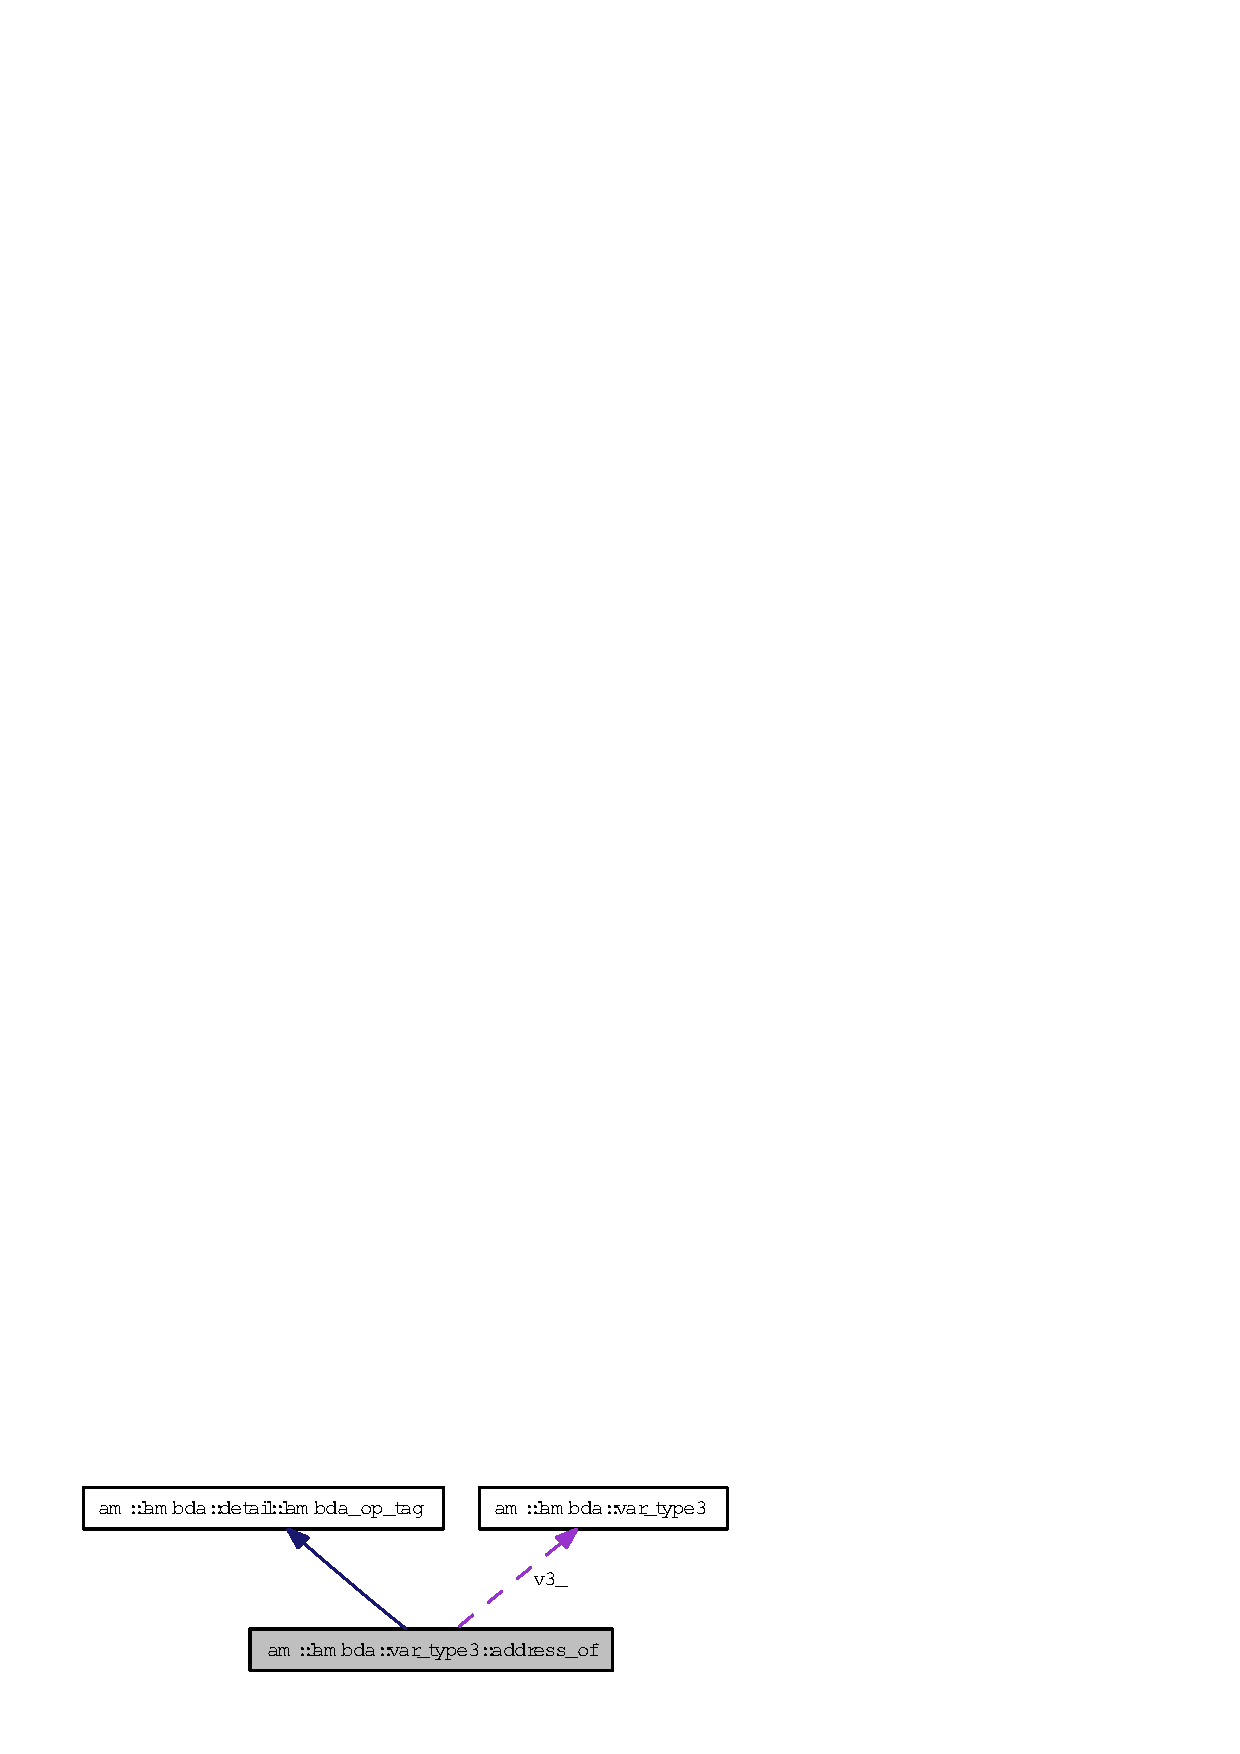
\includegraphics[width=176pt]{structam_1_1lambda_1_1var__type3_1_1address__of__coll__graph}
\end{center}
\end{figure}
\subsection*{Public Member Functions}
\begin{CompactItemize}
\item 
\textbf{address\_\-of} ({\bf var\_\-type3} const \&v3)\label{structam_1_1lambda_1_1var__type3_1_1address__of_6b092d90df186f9f058f2bcd6bc18c67}

\item 
template$<$class T1, class T2, class T3$>$ T3 $\ast$ \textbf{operator()} (T1 \&t1, T2 \&t2, T3 \&t3) const \label{structam_1_1lambda_1_1var__type3_1_1address__of_e8a581a4a10a65726909b080fd7c1102}

\end{CompactItemize}
\subsection*{Public Attributes}
\begin{CompactItemize}
\item 
{\bf var\_\-type3} const \& \textbf{v3\_\-}\label{structam_1_1lambda_1_1var__type3_1_1address__of_903422301692749cd8a6a1b86bc4fcd0}

\end{CompactItemize}


\subsection{Detailed Description}
\begin{Desc}
\item[For internal use only.]
\doxyref{address\_\-of}{p.}{structam_1_1lambda_1_1var__type3_1_1address__of} pure function. Return the address of the variable type 1.

\begin{Desc}
\item[See also:]operator \&() \end{Desc}
\end{Desc}




The documentation for this struct was generated from the following file:\begin{CompactItemize}
\item 
{\bf lambda.hpp}\end{CompactItemize}

\chapter{am::mate File Documentation}
\section{lambda.hpp File Reference}
\label{lambda_8hpp}\index{lambda.hpp@{lambda.hpp}}
Creating an anonymous function object (pure function). 

\subsection*{Namespaces}
\begin{CompactItemize}
\item 
namespace {\bf am}
\item 
namespace {\bf am::lambda}
\item 
namespace \textbf{am::lambda::detail}
\end{CompactItemize}
\subsection*{Classes}
\begin{CompactItemize}
\item 
struct {\bf am::lambda::detail::lambda\_\-op\_\-tag}
\item 
struct {\bf am::lambda::var\_\-type1}
\item 
struct {\bf am::lambda::var\_\-type1::address\_\-of}
\item 
struct {\bf am::lambda::var\_\-type2}
\item 
struct {\bf am::lambda::var\_\-type2::address\_\-of}
\item 
struct {\bf am::lambda::var\_\-type3}
\item 
struct {\bf am::lambda::var\_\-type3::address\_\-of}
\item 
struct {\bf am::lambda::pf\_\-memdata$<$ P, O, U $>$}
\item 
struct {\bf am::lambda::pf\_\-memdata$<$ P, O, U $>$::address\_\-of}
\item 
struct {\bf am::lambda::condition}
\begin{CompactList}\small\item\em Predicate. \item\end{CompactList}\item 
struct {\bf am::lambda::detail::is\_\-lambda\_\-op$<$ T $>$}
\item 
struct \textbf{am::lambda::detail::if\_\-$<$ true, THEN, ELSE $>$}
\item 
struct \textbf{am::lambda::detail::if\_\-$<$ false, THEN, ELSE $>$}
\item 
struct {\bf am::lambda::detail::lambda\_\-val$<$ V $>$}
\item 
struct {\bf am::lambda::detail::tr$<$ V $>$}
\item 
struct {\bf am::lambda::detail::tr$<$ var\_\-type1 $>$}
\item 
struct {\bf am::lambda::detail::tr$<$ var\_\-type2 $>$}
\item 
struct {\bf am::lambda::detail::tr$<$ var\_\-type3 $>$}
\item 
struct \textbf{am::lambda::detail::void\_\-to\_\-default\_\-void$<$ T $>$}
\item 
struct \textbf{am::lambda::detail::void\_\-to\_\-default\_\-void$<$ void $>$}
\item 
struct \textbf{am::lambda::detail::is\_\-$<$ T $>$}
\item 
struct \textbf{am::lambda::detail::is\_\-$<$ T $>$::\_\-pointer\_\-of\_\-$<$ U $>$}
\item 
struct \textbf{am::lambda::detail::is\_\-$<$ T $>$::\_\-reference\_\-of\_\-$<$ U $>$}
\item 
struct \textbf{am::lambda::detail::binder\_\-impl$<$ R $>$}
\item 
struct \textbf{am::lambda::detail::binder\_\-impl$<$ R $>$::select\_\-return$<$$>$}
\item 
struct \textbf{am::lambda::detail::binder\_\-impl$<$ R $>$::select\_\-return$<$$>$::invoke\_\-on\_\-pointer}
\item 
struct \textbf{am::lambda::detail::binder\_\-impl$<$ R $>$::select\_\-return$<$$>$::invoke\_\-on\_\-object}
\item 
struct {\bf am::lambda::binder\_\-obj0$<$ R, U, A1 $>$}
\item 
struct {\bf am::lambda::binder\_\-const\_\-obj0$<$ R, U, A1 $>$}
\item 
struct {\bf am::lambda::binder\_\-obj1$<$ R, P1, U, A1, A2 $>$}
\item 
struct {\bf am::lambda::binder\_\-const\_\-obj1$<$ R, P1, U, A1, A2 $>$}
\item 
struct {\bf am::lambda::binder\_\-obj2$<$ R, P1, P2, U, A1, A2, A3 $>$}
\item 
struct {\bf am::lambda::binder\_\-const\_\-obj2$<$ R, P1, P2, U, A1, A2, A3 $>$}
\item 
struct {\bf am::lambda::binder\_\-obj3$<$ R, P1, P2, P3, U, A1, A2, A3, A4 $>$}
\item 
struct {\bf am::lambda::binder\_\-const\_\-obj3$<$ R, P1, P2, P3, U, A1, A2, A3, A4 $>$}
\item 
struct {\bf am::lambda::binder0$<$ R $>$}
\item 
struct {\bf am::lambda::binder1$<$ R, P1, A1 $>$}
\item 
struct {\bf am::lambda::binder2$<$ R, P1, P2, A1, A2 $>$}
\item 
struct {\bf am::lambda::binder3$<$ R, P1, P2, P3, A1, A2, A3 $>$}
\end{CompactItemize}
\subsection*{Defines}
\begin{CompactItemize}
\item 
\#define \textbf{\_\-\_\-LAMBDA\_\-HPP\_\-\_\-INCLUDED\_\-\_\-}\label{lambda_8hpp_d07b71d47578d363a02f00922be41cb1}

\item 
\#define {\bf UNARY\_\-BOOL\_\-OP}(NAME, OP)
\item 
\#define {\bf BINARY\_\-BOOL\_\-OP}(NAME, OP)
\end{CompactItemize}
\subsection*{Typedefs}
\begin{CompactItemize}
\item 
typedef void \textbf{am::lambda::detail::default\_\-void}\label{namespaceam_1_1lambda_1_1detail_3b0afad9dbbb6961d3fe3dbf260ae010}

\end{CompactItemize}
\subsection*{Functions}
\begin{CompactItemize}
\item 
template$<$class P, class O, class U$>$ pf\_\-memdata$<$ P, O, U $>$ {\bf am::lambda::operator $\rightarrow$  $\ast$} (P opnd, U(O::$\ast$pu))
\item 
template$<$typename R, typename U, typename A1$>$ binder\_\-obj0$<$ R, U, typename detail::tr$<$ A1 $>$::type $>$ {\bf am::lambda::bind} (R(U::$\ast$mfn)(), A1 a1)
\item 
template$<$typename R, typename P1, typename U, typename A1, typename A2$>$ binder\_\-obj1$<$ R, P1, U, typename detail::tr$<$ A1 $>$::type, typename detail::tr$<$ A2 $>$::type $>$ {\bf am::lambda::bind} (R(U::$\ast$mfn)(P1), A1 a1, A2 a2)
\item 
template$<$typename R, typename P1, typename P2, typename U, typename A1, typename A2, typename A3$>$ binder\_\-obj2$<$ R, P1, P2, U, typename detail::tr$<$ A1 $>$::type, typename detail::tr$<$ A2 $>$::type, typename detail::tr$<$ A3 $>$::type $>$ {\bf am::lambda::bind} (R(U::$\ast$mfn)(P1, P2), A1 a1, A2 a2, A3 a3)
\item 
template$<$typename R, typename P1, typename P2, typename P3, typename U, typename A1, typename A2, typename A3, typename A4$>$ binder\_\-obj3$<$ R, P1, P2, P3, U, typename detail::tr$<$ A1 $>$::type, typename detail::tr$<$ A2 $>$::type, typename detail::tr$<$ A3 $>$::type, typename detail::tr$<$ A4 $>$::type $>$ {\bf am::lambda::bind} (R(U::$\ast$mfn)(P1, P2, P3), A1 a1, A2 a2, A3 a3, A4 a4)
\item 
template$<$typename R$>$ binder0$<$ R $>$ {\bf am::lambda::bind} (R($\ast$fn)())
\item 
template$<$typename R, typename P1, typename A1$>$ binder1$<$ R, P1, typename detail::tr$<$ A1 $>$::type $>$ {\bf am::lambda::bind} (R($\ast$fn)(P1), A1 a1)
\item 
template$<$typename R, typename P1, typename P2, typename A1, typename A2$>$ binder2$<$ R, P1, P2, typename detail::tr$<$ A1 $>$::type, typename detail::tr$<$ A2 $>$::type $>$ {\bf am::lambda::bind} (R($\ast$fn)(P1, P2), A1 a1, A2 a2)
\item 
template$<$typename R, typename P1, typename P2, typename P3, typename A1, typename A2, typename A3$>$ binder3$<$ R, P1, P2, P3, typename detail::tr$<$ A1 $>$::type, typename detail::tr$<$ A2 $>$::type, typename detail::tr$<$ A3 $>$::type $>$ {\bf am::lambda::bind} (R($\ast$fn)(P1, P2, P3), A1 a1, A2 a2, A3 a3)
\end{CompactItemize}
\subsection*{Variables}
\begin{CompactItemize}
\item 
static var\_\-type1 {\bf am::lambda::\_\-1}\label{namespaceam_1_1lambda_46cdab44274e0a15a02179cade2f0bb4}

\begin{CompactList}\small\item\em 1st lambda place holder. \item\end{CompactList}\item 
static var\_\-type2 {\bf am::lambda::\_\-2}\label{namespaceam_1_1lambda_be9e932c0d9cdc2f591c5909be5540f3}

\begin{CompactList}\small\item\em 2nd lambda place holder. \item\end{CompactList}\item 
static var\_\-type3 {\bf am::lambda::\_\-3}\label{namespaceam_1_1lambda_1d4c5fedf2e7cdfc66c96e25990a39a6}

\begin{CompactList}\small\item\em 3rd lambda place holder. \item\end{CompactList}\end{CompactItemize}


\subsection{Detailed Description}
Creating an anonymous function object (pure function). 

\begin{Desc}
\item[Author:]Jae\-Wook Choi (zzzz.ooo \char`\"{}at' gmail.com) \end{Desc}
\begin{Desc}
\item[Version:]1.01 \end{Desc}
\begin{Desc}
\item[Date:]12.12.2006 \end{Desc}
\begin{Desc}
\item[Warning:]This software is provided \char`\"{}as is\char`\"{} without express or implied warranty. 

Use it at your own risk! \end{Desc}


\subsection{Define Documentation}
\index{lambda.hpp@{lambda.hpp}!BINARY_BOOL_OP@{BINARY\_\-BOOL\_\-OP}}
\index{BINARY_BOOL_OP@{BINARY\_\-BOOL\_\-OP}!lambda.hpp@{lambda.hpp}}
\subsubsection{\setlength{\rightskip}{0pt plus 5cm}\#define BINARY\_\-BOOL\_\-OP(NAME, OP)}\label{lambda_8hpp_3705a18f2aa3aec04833a934da1226ac}


\textbf{Value:}

\begin{Code}\begin{verbatim}template<class L, class R> struct NAME : public detail::lambda_op_tag \
{ \
  L lhs_; R rhs_; \
  NAME(L lhs, R rhs) : lhs_( lhs ), rhs_( rhs ) { } \
  template<class T1, class T2, class T3> bool operator ()(T1 t1, T2 t2, T3 t3) const { return lhs_( t1, t2, t3 ) OP rhs_( t1, t2, t3 ); } \
  template<class T1, class T2> bool operator ()(T1 t1, T2 t2) const { return lhs_( t1, t2 ) OP rhs_( t1, t2 ); } \
  template<class T1> bool operator ()(T1 t1) const { return lhs_( t1 ) OP rhs_( t1 ); } \
  bool operator ()() const { return lhs_() OP rhs_(); } \
}; \
template<class L, class R> inline \
NAME<typename detail::tr<L>::type, typename detail::tr<R>::type> \
operator OP(L lhs, R rhs) \
{ \
  typedef typename detail::tr<L>::type lhs_type; \
  typedef typename detail::tr<R>::type rhs_type; \
  return NAME<lhs_type, rhs_type>( lhs_type( lhs ), rhs_type( rhs ) ); \
}
\end{verbatim}\end{Code}
\begin{Desc}
\item[For internal use only.]
Defines a binary boolean lambda operator functor, {\em NAME\/} and its helper operator overloading, {\em OP\/}.



\begin{Code}\begin{verbatim} BINARY_BOOL_OP( pf_eq, == ) 
\end{verbatim}\end{Code}



generates the equivalent code snippet as shown below,



\begin{Code}\begin{verbatim} template<class L, class R> struct pf_eq : public detail::lambda_op_tag
 {
   L lhs_; R rhs_;
   pf_eq(L lhs, R rhs) : lhs_( lhs ), rhs_( rhs ) { }
   template<class T1, class T2, class T3> bool operator ()(T1 t1, T2 t2, T3 t3) const { return lhs_( t1, t2, t3 ) == rhs_( t1, t2, t3 ); }
   template<class T1, class T2> bool operator ()(T1 t1, T2 t2) const { return lhs_( t1, t2 ) == rhs_( t1, t2 ); }
   template<class T1> bool operator ()(T1 t1) const { return lhs_( t1 ) == rhs_( t1 ); }
   bool operator ()() const { return lhs_() == rhs_(); }
 };
 template<class L, class R> inline
 pf_eq<typename detail::tr<L>::type, typename detail::tr<R>::type>
 operator ==(L lhs, R rhs)
 {
   typedef typename detail::tr<L>::type lhs_type;
   typedef typename detail::tr<R>::type rhs_type;
   return pf_eq<lhs_type, rhs_type>( lhs_type( lhs ), rhs_type( rhs ) );
 }
\end{verbatim}\end{Code}

 \end{Desc}
\index{lambda.hpp@{lambda.hpp}!UNARY_BOOL_OP@{UNARY\_\-BOOL\_\-OP}}
\index{UNARY_BOOL_OP@{UNARY\_\-BOOL\_\-OP}!lambda.hpp@{lambda.hpp}}
\subsubsection{\setlength{\rightskip}{0pt plus 5cm}\#define UNARY\_\-BOOL\_\-OP(NAME, OP)}\label{lambda_8hpp_ef5d1af95ba871af311cd9c537d8df73}


\textbf{Value:}

\begin{Code}\begin{verbatim}template<class P> struct NAME : public detail::lambda_op_tag \
{ \
  P opnd_; \
  NAME(P opnd) : opnd_( opnd ) { } \
  template<class T1, class T2, class T3> bool operator ()(T1 t1, T2 t2, T3 t3) const { return OP opnd_( t1, t2, t3 ); } \
  template<class T1, class T2> bool operator ()(T1 t1, T2 t2) const { return OP opnd_( t1, t2 ); } \
  template<class T1> bool operator ()(T1 t1) const { return OP opnd_( t1 ); } \
  bool operator()() const { return OP opnd_(); } \
}; \
template<class P> inline \
NAME<typename detail::tr<P>::type> \
operator OP(P opnd) \
{ \
  typedef typename detail::tr<P>::type opnd_type; \
  return NAME<opnd_type>( opnd_type( opnd ) ); \
}
\end{verbatim}\end{Code}
\begin{Desc}
\item[For internal use only.]
Defines an unary boolean lambda operator functor, {\em NAME\/} and its helper operator overloading, {\em OP\/}.



\begin{Code}\begin{verbatim} UNARY_BOOL_OP( pf_not, ! ) 
\end{verbatim}\end{Code}



generates the equivalent code snippet as shown below,



\begin{Code}\begin{verbatim} template<class P> struct pf_not : public detail::lambda_op_tag
 {
   P opnd_;
   pf_not(P opnd) : opnd_( opnd ) { }
   template<class T1, class T2, class T3> bool operator ()(T1 t1, T2 t2, T3 t3) const { return ! opnd_( t1, t2, t3 ); }
   template<class T1, class T2> bool operator ()(T1 t1, T2 t2) const { return ! opnd_( t1, t2 ); }
   template<class T1> bool operator ()(T1 t1) const { return ! opnd_( t1 ); }
   bool operator ()() const { return ! opnd_(); }
 };
 template<class P> inline
 pf_not<typename detail::tr<P>::type>
 operator !(P opnd)
 {
   typedef typename detail::tr<P>::type opnd_type;
   return pf_not<opnd_type>( opnd_type( opnd ) );
 }
\end{verbatim}\end{Code}

 \end{Desc}

\section{mate.hpp File Reference}
\label{mate_8hpp}\index{mate.hpp@{mate.hpp}}
Writing an exception safe code in generic way. 

\subsection*{Namespaces}
\begin{CompactItemize}
\item 
namespace {\bf am}
\item 
namespace \textbf{am::detail}
\end{CompactItemize}
\subsection*{Classes}
\begin{CompactItemize}
\item 
class {\bf am::detail::mate\_\-base}
\item 
class {\bf am::detail::simple\_\-ptr\_\-holder}
\item 
struct \textbf{am::detail::simple\_\-ptr\_\-holder::typed\_\-$<$ T $>$}
\item 
class {\bf am::mate$<$ R $>$}
\begin{CompactList}\small\item\em Mates a host function with the mate function object. \item\end{CompactList}\item 
struct {\bf am::mate$<$ R $>$::typed\_\-$<$ T $>$}
\item 
class {\bf am::mate$<$ void $>$}
\begin{CompactList}\small\item\em void template specialization for mate. \item\end{CompactList}\item 
struct {\bf am::mate$<$ void $>$::typed\_\-$<$ T $>$}
\item 
struct {\bf am::condition}
\begin{CompactList}\small\item\em Predicate. \item\end{CompactList}\item 
class {\bf am::ref\_\-holder$<$ T $>$}
\begin{CompactList}\small\item\em Reference holder. \item\end{CompactList}\item 
struct {\bf am::pointer\_\-to\_\-function$<$ Fn $>$}
\begin{CompactList}\small\item\em Function pointer to an unary function or a binary function. \item\end{CompactList}\item 
struct {\bf am::binder1st$<$ Op, P1 $>$}
\begin{CompactList}\small\item\em Bind the 1st argument of a binary function. \item\end{CompactList}\item 
struct {\bf am::binder2nd$<$ Op, P2 $>$}
\begin{CompactList}\small\item\em Bind the 2nd argument of a binary function. \item\end{CompactList}\end{CompactItemize}
\subsection*{Defines}
\begin{CompactItemize}
\item 
\#define \textbf{\_\-\_\-MATE\_\-HPP\_\-\_\-INCLUDED\_\-\_\-}\label{mate_8hpp_3e4350f057eab99f651bf44d03762124}

\item 
\#define \textbf{AM\_\-JOIN}(a, b)~AM\_\-DO\_\-JOIN(a, b)\label{mate_8hpp_f20ae84ff5fe6051ab485fe2188d1764}

\item 
\#define \textbf{AM\_\-DO\_\-JOIN}(a, b)~AM\_\-DO\_\-JOIN2(a, b)\label{mate_8hpp_ef14a56f5094b52719cef7b4babbb19c}

\item 
\#define \textbf{AM\_\-DO\_\-JOIN2}(a, b)~a\#\#b\label{mate_8hpp_252890d60fe1730841c5a00489165ec4}

\item 
\#define {\bf AM\_\-ANONYMOUS\_\-MATE}(HOST\_\-FN, MATE\_\-FN, UNIQUE)
\item 
\#define {\bf AM\_\-ANONYMOUS\_\-MATE\_\-IF}(HOST\_\-FN, MATE\_\-FN, COND, UNIQUE)
\item 
\#define {\bf AM\_\-ANONYMOUS\_\-MATE\_\-VOID}(MATE\_\-FN, UNIQUE)
\item 
\#define {\bf AM\_\-ANONYMOUS\_\-MATE\_\-VOID\_\-IF}(MATE\_\-FN, COND, UNIQUE)
\item 
\#define {\bf MATE}(HOST\_\-FN, MATE\_\-FN)~AM\_\-ANONYMOUS\_\-MATE(HOST\_\-FN, MATE\_\-FN, \_\-\_\-LINE\_\-\_\-)
\item 
\#define {\bf MATE\_\-IF}(HOST\_\-FN, MATE\_\-FN, COND)~AM\_\-ANONYMOUS\_\-MATE\_\-IF(HOST\_\-FN, MATE\_\-FN, COND, \_\-\_\-LINE\_\-\_\-)
\item 
\#define {\bf MATE\_\-VOID}(MATE\_\-FN)~AM\_\-ANONYMOUS\_\-MATE\_\-VOID(MATE\_\-FN, \_\-\_\-LINE\_\-\_\-)
\item 
\#define {\bf MATE\_\-VOID\_\-IF}(MATE\_\-FN, COND)~AM\_\-ANONYMOUS\_\-MATE\_\-VOID\_\-IF(MATE\_\-FN, COND, \_\-\_\-LINE\_\-\_\-)
\item 
\#define {\bf MATE\_\-}(N, HOST\_\-FN, MATE\_\-FN)~MATE(HOST\_\-FN, MATE\_\-FN)
\item 
\#define {\bf MATE\_\-IF\_\-}(N, HOST\_\-FN, MATE\_\-FN, COND)~MATE\_\-IF(HOST\_\-FN, MATE\_\-FN, COND)
\item 
\#define {\bf MATE\_\-VOID\_\-}(N, MATE\_\-FN)~MATE\_\-VOID(MATE\_\-FN)
\item 
\#define {\bf MATE\_\-VOID\_\-IF\_\-}(N, MATE\_\-FN, COND)~MATE\_\-VOID\_\-IF(MATE\_\-FN, COND)
\end{CompactItemize}
\subsection*{Functions}
\begin{CompactItemize}
\item 
template$<$class R, class T$>$ mate$<$ R $>$ {\bf am::make\_\-mate} (R ret, T mate\_\-functor)
\item 
template$<$class R, class T, class C$>$ mate$<$ R $>$ {\bf am::make\_\-mate} (R ret, T mate\_\-functor, C mate\_\-if)
\item 
template$<$class T$>$ ref\_\-holder$<$ T $>$ {\bf am::ref} (T \&ref)
\item 
template$<$class T$>$ ref\_\-holder$<$ T const $>$ {\bf am::cref} (T const \&ref)
\item 
template$<$typename Fn$>$ pointer\_\-to\_\-function$<$ Fn $>$ {\bf am::ptr\_\-fun} (Fn const fn)
\item 
template$<$typename Op, typename P1$>$ binder1st$<$ Op, P1 $>$ {\bf am::bind1st} (Op const \&op, P1 p1)
\item 
template$<$typename Op, typename P2$>$ binder2nd$<$ Op, P2 $>$ {\bf am::bind2nd} (Op const \&op, P2 p2)
\end{CompactItemize}


\subsection{Detailed Description}
Writing an exception safe code in generic way. 

\begin{Desc}
\item[Author:]Jae\-Wook Choi (zzzz.ooo \char`\"{}at' gmail.com) \end{Desc}
\begin{Desc}
\item[Version:]1.02 \end{Desc}
\begin{Desc}
\item[Date:]12.12.2006 \end{Desc}
\begin{Desc}
\item[Warning:]This software is provided \char`\"{}as is\char`\"{} without express or implied warranty. 

Use it at your own risk! \end{Desc}


\subsection{Define Documentation}
\index{mate.hpp@{mate.hpp}!AM_ANONYMOUS_MATE@{AM\_\-ANONYMOUS\_\-MATE}}
\index{AM_ANONYMOUS_MATE@{AM\_\-ANONYMOUS\_\-MATE}!mate.hpp@{mate.hpp}}
\subsubsection{\setlength{\rightskip}{0pt plus 5cm}\#define AM\_\-ANONYMOUS\_\-MATE(HOST\_\-FN, MATE\_\-FN, UNIQUE)}\label{mate_8hpp_0b43846b9d4b2cf0017afdb28a0fdda6}


\textbf{Value:}

\begin{Code}\begin{verbatim}am::detail::mate_base const & AM_JOIN(_anonymous_, UNIQUE) = \
  am::make_mate((HOST_FN), (MATE_FN)); AM_JOIN(_anonymous_, UNIQUE);
\end{verbatim}\end{Code}
\begin{Desc}
\item[For internal use only.]
Generates anonymous mate variable. \end{Desc}
\index{mate.hpp@{mate.hpp}!AM_ANONYMOUS_MATE_IF@{AM\_\-ANONYMOUS\_\-MATE\_\-IF}}
\index{AM_ANONYMOUS_MATE_IF@{AM\_\-ANONYMOUS\_\-MATE\_\-IF}!mate.hpp@{mate.hpp}}
\subsubsection{\setlength{\rightskip}{0pt plus 5cm}\#define AM\_\-ANONYMOUS\_\-MATE\_\-IF(HOST\_\-FN, MATE\_\-FN, COND, UNIQUE)}\label{mate_8hpp_a986ab16c039b02db09e4da015c65a0d}


\textbf{Value:}

\begin{Code}\begin{verbatim}am::detail::mate_base const & AM_JOIN(_anonymous_if_, UNIQUE) = \
  am::make_mate((HOST_FN), (MATE_FN), (COND)); AM_JOIN(_anonymous_if_, UNIQUE);
\end{verbatim}\end{Code}
\begin{Desc}
\item[For internal use only.]
Generates anonymous mate variable with a condition. \end{Desc}
\index{mate.hpp@{mate.hpp}!AM_ANONYMOUS_MATE_VOID@{AM\_\-ANONYMOUS\_\-MATE\_\-VOID}}
\index{AM_ANONYMOUS_MATE_VOID@{AM\_\-ANONYMOUS\_\-MATE\_\-VOID}!mate.hpp@{mate.hpp}}
\subsubsection{\setlength{\rightskip}{0pt plus 5cm}\#define AM\_\-ANONYMOUS\_\-MATE\_\-VOID(MATE\_\-FN, UNIQUE)}\label{mate_8hpp_b96c3730f55e6042664d206492749cf3}


\textbf{Value:}

\begin{Code}\begin{verbatim}am::mate<void> AM_JOIN(_anonymous_void_, UNIQUE)((MATE_FN)); \
 AM_JOIN(_anonymous_void_, UNIQUE);
\end{verbatim}\end{Code}
\begin{Desc}
\item[For internal use only.]
Generates anonymous mate$<$void$>$ variable. \end{Desc}
\index{mate.hpp@{mate.hpp}!AM_ANONYMOUS_MATE_VOID_IF@{AM\_\-ANONYMOUS\_\-MATE\_\-VOID\_\-IF}}
\index{AM_ANONYMOUS_MATE_VOID_IF@{AM\_\-ANONYMOUS\_\-MATE\_\-VOID\_\-IF}!mate.hpp@{mate.hpp}}
\subsubsection{\setlength{\rightskip}{0pt plus 5cm}\#define AM\_\-ANONYMOUS\_\-MATE\_\-VOID\_\-IF(MATE\_\-FN, COND, UNIQUE)}\label{mate_8hpp_034dce381d7a40e6b85afa5fc84ed86d}


\textbf{Value:}

\begin{Code}\begin{verbatim}am::mate<void> AM_JOIN(_anonymous_void_if_, UNIQUE)((MATE_FN), (COND)); \
 AM_JOIN(_anonymous_void_if_, UNIQUE);
\end{verbatim}\end{Code}
\begin{Desc}
\item[For internal use only.]
Generates anonymous mate$<$void$>$ variable with a condition. \end{Desc}
\index{mate.hpp@{mate.hpp}!MATE@{MATE}}
\index{MATE@{MATE}!mate.hpp@{mate.hpp}}
\subsubsection{\setlength{\rightskip}{0pt plus 5cm}\#define MATE(HOST\_\-FN, MATE\_\-FN)~AM\_\-ANONYMOUS\_\-MATE(HOST\_\-FN, MATE\_\-FN, \_\-\_\-LINE\_\-\_\-)}\label{mate_8hpp_01562e931d80813b43fcddc1a13799fe}


Create an anonymous (unnamed) mate variable which calls the mate function object, {\em MATE\_\-FN\/} in its destructor with the return of the host function, {\em HOST\_\-FN\/} as its argument when it goes out of scope.

\begin{Desc}
\item[See also:]\doxyref{AM\_\-ANONYMOUS\_\-MATE()}{p.}{mate_8hpp_0b43846b9d4b2cf0017afdb28a0fdda6} \end{Desc}
\index{mate.hpp@{mate.hpp}!MATE_@{MATE\_\-}}
\index{MATE_@{MATE\_\-}!mate.hpp@{mate.hpp}}
\subsubsection{\setlength{\rightskip}{0pt plus 5cm}\#define MATE\_\-(N, HOST\_\-FN, MATE\_\-FN)~MATE(HOST\_\-FN, MATE\_\-FN)}\label{mate_8hpp_19fc8b71e7a27de46d8a4a8c7ef8c3ff}


It is devised to remedy the issue that some compiler can't generate an unique anonymous variable. In such compiler, user must provide an unique number {\em N\/} to create an unique identifier manually. In other compilers, it is identical to \doxyref{MATE()}{p.}{mate_8hpp_01562e931d80813b43fcddc1a13799fe} and {\em N\/} is simply ignored.

\begin{Desc}
\item[See also:]\doxyref{MATE()}{p.}{mate_8hpp_01562e931d80813b43fcddc1a13799fe} \end{Desc}
\index{mate.hpp@{mate.hpp}!MATE_IF@{MATE\_\-IF}}
\index{MATE_IF@{MATE\_\-IF}!mate.hpp@{mate.hpp}}
\subsubsection{\setlength{\rightskip}{0pt plus 5cm}\#define MATE\_\-IF(HOST\_\-FN, MATE\_\-FN, COND)~AM\_\-ANONYMOUS\_\-MATE\_\-IF(HOST\_\-FN, MATE\_\-FN, COND, \_\-\_\-LINE\_\-\_\-)}\label{mate_8hpp_9017d939bd69b57ffa03347874ac607b}


Create an anonymous (unnamed) mate variable which calls the mate function object, {\em MATE\_\-FN\/} in its destructor with the return of the host function {\em HOST\_\-FN\/} as its argument when it goes out of scope only if the unary predicate, {\em COND\/} asserts true.

\begin{Desc}
\item[See also:]\doxyref{AM\_\-ANONYMOUS\_\-MATE\_\-IF()}{p.}{mate_8hpp_a986ab16c039b02db09e4da015c65a0d} \end{Desc}
\index{mate.hpp@{mate.hpp}!MATE_IF_@{MATE\_\-IF\_\-}}
\index{MATE_IF_@{MATE\_\-IF\_\-}!mate.hpp@{mate.hpp}}
\subsubsection{\setlength{\rightskip}{0pt plus 5cm}\#define MATE\_\-IF\_\-(N, HOST\_\-FN, MATE\_\-FN, COND)~MATE\_\-IF(HOST\_\-FN, MATE\_\-FN, COND)}\label{mate_8hpp_4cca2d4ba772910bd738c660c1a8348e}


It is devised to remedy the issue that some compiler can't generate an unique anonymous variable. In such compiler, user must provide an unique number {\em N\/} to create an unique identifier manually. In other compilers, it is identical to \doxyref{MATE\_\-IF()}{p.}{mate_8hpp_9017d939bd69b57ffa03347874ac607b} and {\em N\/} is simply ignored.

\begin{Desc}
\item[See also:]\doxyref{MATE\_\-IF()}{p.}{mate_8hpp_9017d939bd69b57ffa03347874ac607b} \end{Desc}
\index{mate.hpp@{mate.hpp}!MATE_VOID@{MATE\_\-VOID}}
\index{MATE_VOID@{MATE\_\-VOID}!mate.hpp@{mate.hpp}}
\subsubsection{\setlength{\rightskip}{0pt plus 5cm}\#define MATE\_\-VOID(MATE\_\-FN)~AM\_\-ANONYMOUS\_\-MATE\_\-VOID(MATE\_\-FN, \_\-\_\-LINE\_\-\_\-)}\label{mate_8hpp_b64fb21cccc9097c72ddab9f2c37d78a}


Create an anonymous (unnamed) mate variable which calls the mate function object, {\em MATE\_\-FN\/} in its destructor when it goes out of scope.

\begin{Desc}
\item[See also:]\doxyref{AM\_\-ANONYMOUS\_\-MATE\_\-VOID()}{p.}{mate_8hpp_b96c3730f55e6042664d206492749cf3} \end{Desc}
\index{mate.hpp@{mate.hpp}!MATE_VOID_@{MATE\_\-VOID\_\-}}
\index{MATE_VOID_@{MATE\_\-VOID\_\-}!mate.hpp@{mate.hpp}}
\subsubsection{\setlength{\rightskip}{0pt plus 5cm}\#define MATE\_\-VOID\_\-(N, MATE\_\-FN)~MATE\_\-VOID(MATE\_\-FN)}\label{mate_8hpp_c8c88f0150b222ce2afb082872d36918}


It is devised to remedy the issue that some compiler can't generate an unique anonymous variable. In such compiler, user must provide an unique number {\em N\/} to create an unique identifier manually. In other compilers, it is identical to \doxyref{MATE\_\-VOID()}{p.}{mate_8hpp_b64fb21cccc9097c72ddab9f2c37d78a} and {\em N\/} is simply ignored.

\begin{Desc}
\item[See also:]\doxyref{MATE\_\-VOID()}{p.}{mate_8hpp_b64fb21cccc9097c72ddab9f2c37d78a} \end{Desc}
\index{mate.hpp@{mate.hpp}!MATE_VOID_IF@{MATE\_\-VOID\_\-IF}}
\index{MATE_VOID_IF@{MATE\_\-VOID\_\-IF}!mate.hpp@{mate.hpp}}
\subsubsection{\setlength{\rightskip}{0pt plus 5cm}\#define MATE\_\-VOID\_\-IF(MATE\_\-FN, COND)~AM\_\-ANONYMOUS\_\-MATE\_\-VOID\_\-IF(MATE\_\-FN, COND, \_\-\_\-LINE\_\-\_\-)}\label{mate_8hpp_becd3ca3f114b18666fd383aad100fef}


Create an anonymous (unnamed) mate variable which calls the mate function object, {\em MATE\_\-FN\/} in its destructor when it goes out of scope only if the null-nary predicate, {\em COND\/} asserts true.

\begin{Desc}
\item[See also:]\doxyref{AM\_\-ANONYMOUS\_\-MATE\_\-VOID\_\-IF()}{p.}{mate_8hpp_034dce381d7a40e6b85afa5fc84ed86d} \end{Desc}
\index{mate.hpp@{mate.hpp}!MATE_VOID_IF_@{MATE\_\-VOID\_\-IF\_\-}}
\index{MATE_VOID_IF_@{MATE\_\-VOID\_\-IF\_\-}!mate.hpp@{mate.hpp}}
\subsubsection{\setlength{\rightskip}{0pt plus 5cm}\#define MATE\_\-VOID\_\-IF\_\-(N, MATE\_\-FN, COND)~MATE\_\-VOID\_\-IF(MATE\_\-FN, COND)}\label{mate_8hpp_35d3c430642a21a853b08f966bb16895}


It is devised to remedy the issue that some compiler can't generate an unique anonymous variable. In such compiler, user must provide an unique number {\em N\/} to create an unique identifier manually. In other compilers, it is identical to \doxyref{MATE\_\-VOID\_\-IF()}{p.}{mate_8hpp_becd3ca3f114b18666fd383aad100fef} and {\em N\/} is simply ignored.

\begin{Desc}
\item[See also:]\doxyref{MATE\_\-VOID\_\-IF()}{p.}{mate_8hpp_becd3ca3f114b18666fd383aad100fef} \end{Desc}

\chapter{am::mate Page Documentation}
\section{Introduction.}\label{mate_introduction}
Here is an example of a traditional scenario in our daily programming as shown below. We are prone to forget to call some clean up codes when the function has multiple return paths or an exception is thrown in the middle of very complicated constructs.



\begin{Code}\begin{verbatim} void test01()
 {
  char const * lpszFilePath = "c:\\test.dat";

  HANDLE hFile( ::CreateFile( lpszFilePath, GENERIC_WRITE, 0, NULL, OPEN_ALWAYS, 0, NULL ) );

  if( INVALID_HANDLE_VALUE != hFile )
  {

    if( 100 > ::GetFileSize( hFile, NULL ) )
      throw "File size too small!";

    ::CloseHandle( hFile );
  }

  ::DeleteFile( lpszFilePath );
 }
\end{verbatim}\end{Code}



{\tt boost::shared\_\-ptr} can be used to transform the code snippet above in exception safe way. It purely depends on the ability of the {\tt boost::shared\_\-ptr} that it allows for user to provide a custom deleter function object. See more details from {\tt here}.



\begin{Code}\begin{verbatim} #define BOOST_BIND_ENABLE_STDCALL
 #include <boost/bind.hpp>
 #include <boost/shared_ptr.hpp>

 void test02()
 {
   boost::shared_ptr<char const> spFilePath( "c:\\test.dat", &::DeleteFile );

   boost::shared_ptr<void> spFile(
    ::CreateFile( spFilePath.get(), GENERIC_WRITE, 0, NULL, OPEN_ALWAYS, 0, NULL ),
    &::CloseHandle ); // Custom deleter.

   if( INVALID_HANDLE_VALUE != spFile.get() )
   {

     if( 100 > ::GetFileSize( spFile.get(), NULL ) )
       throw "File size too small!";
   }
 }
\end{verbatim}\end{Code}



Writing a code in the exception safe way at object level doesn't require the fancy reference counting feature of {\tt boost::shared\_\-ptr}, but only requires that of the custom deleter function object. Speaking accurately, what we need is an ability to call an arbitrary custom function object in the destructor of our class variable when it goes out of scope. By extracting and combining merits of the existing implementations such as {\tt boost::shared\_\-ptr}, {\tt Scope\-Guard} and etc., here I will like to introduce a small \doxyref{am::mate}{p.}{classam_1_1mate} utility class.



\begin{Code}\begin{verbatim} #include "mate.h"

 void test03()
 {
   am::mate<char const *> lpszFilePath( "c:\\test.dat", &::DeleteFile );

   am::mate<HANDLE> hFile(
    ::CreateFile( lpszFilePath, GENERIC_WRITE, 0, NULL, OPEN_ALWAYS, 0, NULL ), // Host function.
    &::CloseHandle,                                                             // Mate function.
    (HANDLE)INVALID_HANDLE_VALUE != am::lambda::_1 ); // Mates the function only if the condition asserts true.

   // Treats am::mate<HANDLE> as if it is a HANDLE.
   if( INVALID_HANDLE_VALUE != hFile )
   {

     if( 100 > ::GetFileSize( hFile, NULL ) )
       throw "File size too small";
   }
 }
\end{verbatim}\end{Code}



There are several benefits of using \doxyref{am::mate}{p.}{classam_1_1mate} over the existing implementations.

\begin{enumerate}
\item More intuitive and well defined interfaces.\item Accepts any unary custom mate function object which takes the return of the host function as its argument.\item Not like {\tt boost::shared\_\-ptr} is limited only for the pointer type, \doxyref{am::mate}{p.}{classam_1_1mate} works with any data type. i.e. intergral type, floating point type, pointer type and even reference type.\item Implicit conversion to the return type of the host function which cast an illusion that makes an \doxyref{am::mate}{p.}{classam_1_1mate} instance as if it is a stored variable of the return type of the host function.\item Easy, convenient and compiler-warning-free \doxyref{MATE()}{p.}{mate_8hpp_01562e931d80813b43fcddc1a13799fe} macro definitions to create an anonymous \doxyref{am::mate}{p.}{classam_1_1mate} variable.\item Mates functions with a condition.\item Provides a simple set of boolean lambda operations to support composing an anonymous function object for the condition.\item \doxyref{am::mate$<$void$>$}{p.}{classam_1_1mate_3_01void_01_4} specialization when mating a mate function object without any host function call.\item Well standard compliant and portable. Tested on VC6, VC71, VC80, gcc3.4.2.\item No dependency on boost library but works nicely with it.\item Provide \doxyref{am::ptr\_\-fun}{p.}{namespaceam_075d855cc1ab6d87a818e72ed34bc829}, \doxyref{am::bind1st}{p.}{namespaceam_5d35d0139360afc672d2cf1ff279fd83} and \doxyref{am::bind2nd}{p.}{namespaceam_7416ae43749c6a8c08f3a1f8760ae24f} helper template functions that work well for any calling convention (including {\tt \_\-\_\-stdcall}).\item \doxyref{am::lambda::bind}{p.}{namespaceam_1_1lambda_794d3c4a2b7231c36cfc0684fea9bf5e} up to 3 arguments for both free function and member function are provided.\end{enumerate}


\doxyref{[Contents]}{p.}{index_mate_contents} 
\section{Basic usage.}\label{mate_basic_usage}
\subsection{Mating a host function call with a mate function.}\label{mate_basic_usage_mate_bu_s1}
Mating a host function call with a mate function is easy. Provide the host function as the first argument (by calling it) and the mate function as the second argument of the constructor of the \doxyref{am::mate}{p.}{classam_1_1mate} variable. Specifies the return type of the host function explicitly as the template argument of the \doxyref{am::mate}{p.}{classam_1_1mate} when declaring it.

Use \doxyref{MATE()}{p.}{mate_8hpp_01562e931d80813b43fcddc1a13799fe} macro to create an anonymous \doxyref{am::mate}{p.}{classam_1_1mate} variable when you are not concerning about using \doxyref{am::mate}{p.}{classam_1_1mate} variable.



\begin{Code}\begin{verbatim} int prefix(int n) { return n + 100; }
 void suffix(int n) { n -= 100; }

 void test04()
 {
   am::mate<int> nNumber( prefix(123), &suffix );
   assert( 23 == nNumber );

   int nNumber2 = nNumber; // Compile OK!

 #if 0
   nNumber = nNumber2; // Compile error! mate is non-assignable.
   nNumber = 52;       // Compile error! mate is non-assignable.
 #endif

  {
    MATE( prefix( 333 ), &suffix );

  } // calls suffix( 233 ) here

 } // calls suffix( 23 ) here on exit.
\end{verbatim}\end{Code}



An \doxyref{am::mate}{p.}{classam_1_1mate} variable can be treated as a variable of the data type of which is specified as the template parameter when the \doxyref{am::mate}{p.}{classam_1_1mate} variable is declared. This is due to the implict conversion operator to the data type. But also be aware that it is read-only access, which means it behaves like a const variable. i.e. an {\tt am::mate$<$int$>$} variable can be treated as a {\tt const int} variable.\subsection{Composing a mate fuction object.}\label{mate_basic_usage_mate_bu_s2}
Mate function object will take the return of the host function as its only input argument (it should be an unary function object) when it is called. You can use any known techniques to compose and provide an unary custom function object when constructing \doxyref{am::mate}{p.}{classam_1_1mate} variable.



\begin{Code}\begin{verbatim} struct MyReleaseDC
 {
   HWND hwnd_;
   MyReleaseDC(HWND hwnd) : hwnd_( hwnd ) { }
   int operator ()(HDC hdc) const { return ::ReleaseDC( hwnd_, hdc ); }

 };  // struct MyReleaseDC

 struct MySelectObject
 {
   HDC hdc_;
   MySelectObject(HDC hdc) : hdc_( hdc ) { }
   HGDIOBJ operator ()(HGDIOBJ hgdiobj) const { return ::SelectObject( hdc_, hgdiobj ); }

 };  // struct MySelectObject

 void test05(HWND hwnd)
 {
   am::mate<HDC> hdc( ::GetWindowDC( hwnd ), MyReleaseDC( hwnd ) );

   MATE( ::SelectObject( hdc, ::GetStockObject( BLACK_PEN ) ), MySelectObject( hdc ) );
 } 
\end{verbatim}\end{Code}





\begin{Code}\begin{verbatim} #define BOOST_BIND_ENABLE_STDCALL
 #include <boost/bind.hpp>

 void test06(HWND hwnd)
 {
   am::mate<HDC> hdc( ::GetWindowDC( hwnd ), boost::bind( &::ReleaseDC, hwnd, _1 ) );

   MATE( ::SelectObject( hdc, ::GetStockObject( BLACK_PEN ) ), boost::bind( &::SelectObject, hdc, _1 ) );
 }
\end{verbatim}\end{Code}





\begin{Code}\begin{verbatim} void test07(HWND hwnd)
 {
   am::mate<HDC> hdc( ::GetWindowDC( hwnd ), am::bind1st( &::ReleaseDC, hwnd ) );

   MATE( ::SelectObject( hdc, ::GetStockObject( BLACK_PEN ) ), am::bind1st( &::SelectObject, hdc ) );
 }
\end{verbatim}\end{Code}





\begin{Code}\begin{verbatim} #define AM_BIND_ENABLE_STDCALL
 #include "lambda.hpp"

 void test08(HWND hwnd)
 {
   am::mate<HDC> hdc( ::GetWindowDC( hwnd ), am::lambda::bind( &::ReleaseDC, hwnd, am::lambda::_1 ) );

   MATE( ::SelectObject( hdc, ::GetStockObject( BLACK_PEN ) ),
     am::lambda::bind( &::SelectObject, hdc, am::lambda::_1 ) );
 }
\end{verbatim}\end{Code}

\subsection{Mating with a condition.}\label{mate_basic_usage_mate_bu_s3}
Sometime there are cases in which the host function call might be failed and returns the error code as a result. In such cases, the mate function should not be called. Checking the error of the host function call can be easily performed as \doxyref{am::mate}{p.}{classam_1_1mate} variable can be treated as a const variable of the return type of the host function call. Use dismate\_\-mate() member function to dismiss the mate function call.



\begin{Code}\begin{verbatim} void test09()
 {
   am::mate<HANDLE> hEvent( ::CreateEvent( NULL, FALSE, FALSE, NULL ), &::CloseHandle );
   if( hEvent == NULL )
     hEvent.dismiss_mate();

 }
\end{verbatim}\end{Code}



However this approach can not be used with \doxyref{MATE()}{p.}{mate_8hpp_01562e931d80813b43fcddc1a13799fe} macro. Use \doxyref{MATE\_\-IF()}{p.}{mate_8hpp_9017d939bd69b57ffa03347874ac607b} macro instead and provides a unary predicate as the third input argument for a condition. \doxyref{MATE\_\-IF()}{p.}{mate_8hpp_9017d939bd69b57ffa03347874ac607b} utilizes \doxyref{am::mate}{p.}{classam_1_1mate}'s another constructor which takes an unary predicate as its third input argument. If a condition is provided, the mate function will be called, when it goes out of scope, only if the provided unary predicate asserts true.

The unary predicate takes the return of the host function as its only input argument as well. Like mate function object, you can compose a unary predicate in any techniques you know of.



\begin{Code}\begin{verbatim} struct EventCreated
 {
   bool operator ()(HANDLE hevent) const { return NULL != hevent; }

 };  // struct EventCreated

 void test10()
 {
   MATE_IF( ::CreateEvent( NULL, FALSE, FALSE, NULL ), &::CloseHandle,  EventCreated() );

 }
\end{verbatim}\end{Code}



There is one advantage of using \doxyref{am::mate}{p.}{classam_1_1mate} with a condition than without a condition. When a mate function object is stored into the \doxyref{am::mate}{p.}{classam_1_1mate} variable internally, the heap memory allocation is occurred. But if the condition does not hold, nor will the heap memory allocation occur since the mate function will not be called.



\begin{Code}\begin{verbatim} void test11()
 {
   am::mate<HANDLE> hEvent( ::CreateEvent( NULL, FALSE, FALSE, NULL ),
     &::CloseHandle, (HANDLE)NULL != am::lambda::_1 );

 }
\end{verbatim}\end{Code}

\subsection{am::mate$<$void$>$ specialization.}\label{mate_basic_usage_mate_bu_s4}
If the mate function does not concern about the return of the host function which is given as its input argument, you can write a mate fuction object which takes the return of the host function, but then simply ignores it.



\begin{Code}\begin{verbatim} #define RESOURCE_ACQUSITION_SUCCESS 100
 #define RESOURCE_ACQUSITION_FAIL    200

 int AcquireResource(HANDLE hres) { return RESOURCE_ACQUSITION_SUCCESS; }
 void ReleaseResource(HANDLE hres) { }

 struct IgnoreReturnAndReleaseResource
 {
   HANDLE hres_;
   IgnoreReturnAndReleaseResource(HANDLE hres) : hres_( hres ) { }
   void operator ()(int) const { ReleaseResource( hres_ ); }

 };  // struct IgnoreReturnAndReleaseResource

 void test12(HANDLE hres)
 {
   am::mate<int> nResult( AcquireResource( hres ),
     IgnoreReturnAndReleaseResource( hres ), RESOURCE_ACQUSITION_SUCCESS == am::lambda::_1  );

 } // Calls ReleaseResource( hres ) on exit if AcquireResource( hres ) returns RESOURCE_ACQUSITION_SUCCESS
\end{verbatim}\end{Code}



If you use {\tt boost::bind}, {\tt boost::lambda::bind} or \doxyref{am::lambda::bind}{p.}{namespaceam_1_1lambda_794d3c4a2b7231c36cfc0684fea9bf5e} to compose a function object in the way that all of its input arguments are bound. It will automatically create an unary function object that simply ignores the return of the host function, and when it is called, it will call the mate function only with all those bound input arguments.



\begin{Code}\begin{verbatim} #define RESOURCE_ACQUSITION_SUCCESS 100
 #define RESOURCE_ACQUSITION_FAIL    200

 int AcquireResource(HANDLE hres) { return RESOURCE_ACQUSITION_SUCCESS; }
 void ReleaseResource(HANDLE hres) { }

 void test13(HANDLE hres)
 {
   am::mate<int> nResult( AcquireResource( hres ),
     am::lambda::bind( &ReleaseResource, hres ), RESOURCE_ACQUSITION_SUCCESS == am::lambda::_1  );

 }
\end{verbatim}\end{Code}



If the host function is a function with void return or even we don't have a host function to call at all, \doxyref{am::mate$<$void$>$}{p.}{classam_1_1mate_3_01void_01_4} specialization and \doxyref{MATE\_\-VOID()}{p.}{mate_8hpp_b64fb21cccc9097c72ddab9f2c37d78a} macro play a neat role in such cases as \doxyref{am::mate$<$void$>$}{p.}{classam_1_1mate_3_01void_01_4} class' constructors do not take the return of host function as their first argument.



\begin{Code}\begin{verbatim} void AcquireResourceEx(HANDLE hres) { }
 void ReleaseResourceEx(HANDLE hres) { }
 void Cleanup() { }

 void test14(HANDLE hres, int option)
 {
   am::mate<void> cleanup_on_exit( &Cleanup );

   if( 0 == option )
   {
     AcquireResourceEx( hres );
     MATE_VOID( am::lambda::bind( &ReleaseResourceEx, hres ) );

   }
   else if( 1 == option )
   {
     AcquireResourceEx( hres );
     MATE_VOID_IF( am::lambda::bind( &ReleaseResourceEx, hres ), am::condition( NULL != hres ) );

   }
   else if( 2 == option )
   {
     am::mate<void> dummy( ( AcquireResourceEx( hres ), am::lambda::bind( &ReleaseResourceEx, hres ) ) );

   }
   else if( 3 == option )
   {
     am::mate<void> dummy( ( AcquireResourceEx( hres ), am::lambda::bind( &ReleaseResourceEx, hres ) ),
       am::condition( NULL != hres ) );

   }
   else
   {
     MATE_VOID( ( AcquireResourceEx( hres ), am::lambda::bind( &ReleaseResourceEx, hres ) ) );

   }
 }
\end{verbatim}\end{Code}



It is possible to use comma (,) operator between the host function call and the mate function and then wrap them with the nested parenthesis to make it look and feel the same style as non-void \doxyref{am::mate}{p.}{classam_1_1mate}.

\doxyref{[Contents]}{p.}{index_mate_contents} 
\section{Utility classes and their helper template functions.}\label{mate_utility_classes}
\subsection{Supporting parameter by reference: am::ref and am::cref.}\label{mate_utility_classes_mate_uc_s1}
Specifies the reference type as the template argument of the \doxyref{am::mate}{p.}{classam_1_1mate} class if you want to provide the return of the host function as a reference to the mate function.



\begin{Code}\begin{verbatim} int & Increase(int & x) { return ++x; }
 void Decrease(int & x) { --x; }

 void test15(int & refCount)
 {
   am::mate<int &> decreseOnExit( Increase( refCount ), &Decrease );

 } //  Calls Decrease( refCount ) on exit.
\end{verbatim}\end{Code}



By default, a template parameter is passed by value, not by reference. Thus if a mate function provided wants to take the return of the host function as a reference and \doxyref{MATE()}{p.}{mate_8hpp_01562e931d80813b43fcddc1a13799fe} macro definition is used, the specified mate function will be called with the reference to the \char`\"{}copy\char`\"{} of the argument, not with the reference to argument itself, when it goes out of scope since template parameter is passed by value. Use \doxyref{am::ref}{p.}{namespaceam_aeac214784a5e1a16be743677555cb96} or \doxyref{am::cref}{p.}{namespaceam_10096add639d0ba375c58c53aa8ff4a7} function to specify explicitly to use \doxyref{am::ref\_\-holder}{p.}{classam_1_1ref__holder} class transforms a reference into a value.



\begin{Code}\begin{verbatim} void test16(int & refCount)
 {
   MATE( am::ref( Increase( refCount ) ), &Decrease );

 }  //  Calls Decrease( refCount ) on exit.
\end{verbatim}\end{Code}

\subsubsection{Free function pointer: am::ptr\_\-fun.}\label{mate_utility_classes_mate_uc_s2}
\doxyref{am::ptr\_\-fun}{p.}{namespaceam_075d855cc1ab6d87a818e72ed34bc829} is very similar to {\tt std::ptr\_\-fun} that it is used to convert unary and binary function pointers, respectively, into unary and binary adaptable function objects. However they are different in that \doxyref{am::ptr\_\-fun}{p.}{namespaceam_075d855cc1ab6d87a818e72ed34bc829} can convert the function pointers of any calling covention while {\tt std::ptr\_\-fun} can only convert {\tt \_\-\_\-cdecl} function pointers. In general, use {\tt std::ptr\_\-fun} and ignore \doxyref{am::ptr\_\-fun}{p.}{namespaceam_075d855cc1ab6d87a818e72ed34bc829} if you don't concern about calling convention.

\doxyref{am::ptr\_\-fun}{p.}{namespaceam_075d855cc1ab6d87a818e72ed34bc829} and other helper template functions of \doxyref{am::mate}{p.}{classam_1_1mate} are designed to collaborate only with \doxyref{am::mate}{p.}{classam_1_1mate} and its other sibling helper template functions so do not mix use it with helper template functions from STL (such as {\tt std::ptr\_\-fun}, {\tt std::bind1st}, {\tt std::bind2nd} and so on.)

You can also use \doxyref{am::ptr\_\-fun}{p.}{namespaceam_075d855cc1ab6d87a818e72ed34bc829} to resolve overloaded functions manually since the template rules are very strict for type checking and it is not supposed to resolve the resolution of the overloaded functions automatically.



\begin{Code}\begin{verbatim} // Overloaded functions
 void foo(char const *, int) { }
 void foo(int) { }
 void __stdcall foo(char const *) { }

 void __stdcall bar(char const *) { }

 void test17()
 {
   // Provides function template parameter explicitly to resolve overloaded functions.
   MATE( "Hello foo!", am::ptr_fun<void (_stdcall *)(char const *)>( &foo ) );
   MATE( "Hello foo!", am::bind2nd( am::ptr_fun<void (*)(char const *, int)>( &foo ), 123 ) );

   // am::pointer_to_function is not necessary,
   // unless otherwise resolving overloaded functions is required.
   MATE( "Hello bar!", am::ptr_fun( &bar ) );
   MATE( "Hello bar!", &bar );
 }
\end{verbatim}\end{Code}



Be aware that the template parameter is provided as a single function pointer not as individual types from the function signature like STL does. It gives \doxyref{am::ptr\_\-fun}{p.}{namespaceam_075d855cc1ab6d87a818e72ed34bc829} and its sibling helper template functions the ability to resolve overloaded functions better as well as to work well with any calling conventions but it also prevents from being able to define the public interfaces such as {\tt first\_\-argument\_\-type}, {\tt second\_\-argument\_\-type} and {\tt result\_\-type}. Actually {\tt result\_\-type} is always fixed and defined as void internally since \doxyref{am::mate}{p.}{classam_1_1mate} does not utilize the {\tt result\_\-type} under the hood.

{\bf - NOTE -}

{\em Do {\bf NOT} use \doxyref{am::ptr\_\-fun}{p.}{namespaceam_075d855cc1ab6d87a818e72ed34bc829}, \doxyref{am::bind1st}{p.}{namespaceam_5d35d0139360afc672d2cf1ff279fd83}, \doxyref{am::bind2nd}{p.}{namespaceam_7416ae43749c6a8c08f3a1f8760ae24f} to create a function object which wraps a free function with the calling convention other than {\tt \_\-\_\-cdecl} under none-MSVC environment. Calling convention is subject to be a platform specific therefore it does not work well for none-MSVC environment, especially when function pointer is passed as a template parameter. Use \doxyref{am::lambda::bind}{p.}{namespaceam_1_1lambda_794d3c4a2b7231c36cfc0684fea9bf5e} instead.\/}\subsubsection{Bind the 1st or the 2nd argument of the binary function: am::bind1st and am::bind2nd.}\label{mate_utility_classes_mate_uc_s3}
\doxyref{am::bind1st}{p.}{namespaceam_5d35d0139360afc672d2cf1ff279fd83} and \doxyref{am::bind2nd}{p.}{namespaceam_7416ae43749c6a8c08f3a1f8760ae24f} are similar to {\tt std::bind1st} and {\tt std::bind2nd} respectively but they resolve overloaded functions better as well as work for any calling conventions at the expense of not having public interface {\tt first\_\-argument\_\-type}. The template parameter is also required to be provided as a single function pointer not as individual types from the function signature when resolving overloaded functions is needed.



\begin{Code}\begin{verbatim} void foo(char const *, int) { }
 void __stdcall bar(char const *, int) { }  // __stdcall calling convention.

 void main()
 {
   // MATE( "Hello foo!", std::bind2nd( &foo, 123 ) ); // Compiles error!
   // MATE( "Hello bar!", std::bind2nd( &bar, 123 ) ); // Compiles error!
   MATE( "Hello foo!", am::bind2nd( &foo, 123 ) ); // Compiles OK!
   MATE( "Hello bar!", am::bind2nd( &bar, 123 ) ); // Compiles OK!
 }
\end{verbatim}\end{Code}

\subsubsection{Miscellaneous.}\label{mate_utility_classes_mate_uc_s4}
\doxyref{am::condition}{p.}{structam_1_1condition} can be used to convert a boolean expression into a null-nary or unary predicate.



\begin{Code}\begin{verbatim} void test19(bool cond)
 {
   assert( false == am::condition( 2 == 3 )() );
   assert( false == am::condition( 2 == 3 )( "123" ) );  // Input argument is simply ignored.

   // Use am::lambda::condition instead when composing a function object using am::lambda
   MATE_IF( ::CreateMutex(NULL, TRUE, NULL), &::ReleaseMutex,
     (HANDLE)NULL != am::lambda::_1 && am::lambda::condition( cond ) );
 } 
\end{verbatim}\end{Code}



\doxyref{[Contents]}{p.}{index_mate_contents} 
\section{Use am::lambda to compose a function object.}\label{mate_use_lambda}
{\tt boost::lambda} library provide a very powerful ability to create an anonymous function object on the spot. Unfortunately it does not support some outdated compilers which are still widely being used. In such environment, you can consider to use \doxyref{am::lambda}{p.}{namespaceam_1_1lambda}.

\doxyref{am::lambda}{p.}{namespaceam_1_1lambda} is a limited subset of {\tt boost::lambda} which only supports the following operators.

\begin{itemize}
\item Logical NOT : !\item Logical AND : \&\&\item Logical OR : $|$$|$\item Equality operators : ==, !=\item Relational operators : $<$, $>$, $<$=, $>$=\item Address-of operator : \&\item Pointer-to-member operator : -$>$$\ast$ (to access member data pointer, not member function pointer and read-only access)\end{itemize}


The above lambda operators seems good enough to collaborate with \doxyref{am::mate}{p.}{classam_1_1mate} and, most of all, it might work for those outdated compiler which {\tt boost::lambda} does not support.

Also \doxyref{am::lambda::bind}{p.}{namespaceam_1_1lambda_794d3c4a2b7231c36cfc0684fea9bf5e} overloaded helper template functions are provided to support arguments binding similar to {\tt boost::lambda::bind}.



\begin{Code}\begin{verbatim} #include "mate.hpp"
 #include "lambda.hpp"

 class Graph { };

 std::pair<bool, unsigned> AddVertex(Graph & g)
 {
   bool is_success = false;
   unsigned vertex_descriptor = 0;

   // Add a new vertex.

   // return Pair of boolean success flag and the new vertex descriptor if it
   // successfully added a new vertex.
   return std::make_pair( is_success, vertex_descriptor );
 }

 void RemoveVertex(unsigned vertex_descriptor, Graph & g)
 {
   // Remove the vertex of the specified descriptor.
 }

 void test20(Graph & g)
 {
   typedef std::pair<bool, unsigned> result_pair;

   // 1. Calls the host function AddVertex()
   // 2. Mates RemoveVertex() with the second of the resultant std::pair of the host function
   //    only if the first of the resultant std::pair of the host functio hold true.
   MATE_IF( AddVertex( g ),
     am::lambda::bind( &RemoveVertex, &am::lambda::_1->*&result_pair::second, g ), 
     &am::lambda::_1->*&result_pair::first );
  }
\end{verbatim}\end{Code}



\doxyref{am::lambda::bind}{p.}{namespaceam_1_1lambda_794d3c4a2b7231c36cfc0684fea9bf5e} can resolve overloaded free functions (non-member functions) with {\tt \_\-\_\-stdcall} calling convention when AM\_\-ENABLE\_\-BIND\_\-STDCALL is defined before including, directly or indirectly, \char`\"{}lambda.hpp\char`\"{}. \doxyref{am::lambda::bind}{p.}{namespaceam_1_1lambda_794d3c4a2b7231c36cfc0684fea9bf5e} supports binding only up to 3 input arguments.



\begin{Code}\begin{verbatim} #include "mate.hpp"

 #define AM_BIND_ENABLE_STDCALL
 #include "lambda.hpp"

 typedef std::map<int, RECT> RECT_MAP; // Rect id -> Rectangle
 typedef RECT_MAP::value_type MAP_VALUE;

 MAP_VALUE ModifyRectangle(MAP_VALUE map_value) { return map_value; }
 void UndoRectangle(int rect_id) { }

 void test21(RECT_MAP const & rect_map, POINT pt)
 {
   RECT_MAP::const_iterator it = rect_map.begin(), it_e = rect_map.end();
   for( ; it != it_e; ++it )
   {
     // 1. Calls the host function ModifyRectangle()
     // 2. Mates UndoRectangle() with the first of the iterating map value that
     //    host function returns, only if the rectangle is found to contain the
     //    specified point and the specified point is not the origin (0, 0).
     MATE_IF( ModifyRectangle( *it ),
       am::lambda::bind( &UndoRectangle, &am::lambda::_1->*&MAP_VALUE::first ),
       am::lambda::bind( &::PtInRect, &( &am::lambda::_1->*&MAP_VALUE::second ), pt ) &&
       am::lambda::condition( 0 != pt.x && 0 != pt.y ) );
   }
 }
\end{verbatim}\end{Code}



\doxyref{am::lambda}{p.}{namespaceam_1_1lambda} is completely independent on \doxyref{am::mate}{p.}{classam_1_1mate} and vice-versa, thus both can be used separately.

\doxyref{[Contents]}{p.}{index_mate_contents} 
\section{References.}\label{mate_references}
\begin{enumerate}
\item {\tt CAuto\-Mate$<$$>$: a tiny utility class to run a mate function automatically in code block.}\item {\tt Generic: Change the Way You Write Exception-Safe Code ?Forever.}\item {\tt boost 2: shared\_\-ptr wraps resource handles by peterchen.}\item {\tt Using shared\_\-ptr to execute code on block exit.}\end{enumerate}


\doxyref{[Contents]}{p.}{index_mate_contents} 
\section{Creating an anonymous function object (pure function).}\label{lambda_operations}
\label{lambda_operations_lambda_contents}


\begin{enumerate}
\item \doxyref{Introduction.}{p.}{lambda_operations_lambda_introduction}\item \doxyref{Basic Usage.}{p.}{lambda_operations_lambda_basic_usage}\item \doxyref{Advanced Usage.}{p.}{lambda_operations_lambda_advanced_usage}\item \doxyref{References.}{p.}{lambda_operations_lambda_references}\end{enumerate}
\subsection{Introduction.}\label{lambda_operations_lambda_introduction}
continued...

\doxyref{[top]}{p.}{lambda_operations_lambda_contents}\subsection{Basic Usage.}\label{lambda_operations_lambda_basic_usage}
continued...

\doxyref{[top]}{p.}{lambda_operations_lambda_contents}\subsection{Advanced Usage.}\label{lambda_operations_lambda_advanced_usage}
continued...

\doxyref{[top]}{p.}{lambda_operations_lambda_contents}\subsection{References.}\label{lambda_operations_lambda_references}
\begin{enumerate}
\item {\tt Anonymous function object creation.}\end{enumerate}


\doxyref{[top]}{p.}{lambda_operations_lambda_contents} 
\printindex
\end{document}
